\documentclass[twoside]{book}

% Packages required by doxygen
\usepackage{calc}
\usepackage{doxygen}
\usepackage{graphicx}
\usepackage[utf8]{inputenc}
\usepackage{makeidx}
\usepackage{multicol}
\usepackage{multirow}
\usepackage{textcomp}
\usepackage[table]{xcolor}

% Font selection
\usepackage[T1]{fontenc}
\usepackage{mathptmx}
\usepackage[scaled=.90]{helvet}
\usepackage{courier}
\usepackage{amssymb}
\usepackage{sectsty}
\renewcommand{\familydefault}{\sfdefault}
\allsectionsfont{%
  \fontseries{bc}\selectfont%
  \color{darkgray}%
}
\renewcommand{\DoxyLabelFont}{%
  \fontseries{bc}\selectfont%
  \color{darkgray}%
}

% Page & text layout
\usepackage{geometry}
\geometry{%
  a4paper,%
  top=2.5cm,%
  bottom=2.5cm,%
  left=2.5cm,%
  right=2.5cm%
}
\tolerance=750
\hfuzz=15pt
\hbadness=750
\setlength{\emergencystretch}{15pt}
\setlength{\parindent}{0cm}
\setlength{\parskip}{0.2cm}
\makeatletter
\renewcommand{\paragraph}{%
  \@startsection{paragraph}{4}{0ex}{-1.0ex}{1.0ex}{%
    \normalfont\normalsize\bfseries\SS@parafont%
  }%
}
\renewcommand{\subparagraph}{%
  \@startsection{subparagraph}{5}{0ex}{-1.0ex}{1.0ex}{%
    \normalfont\normalsize\bfseries\SS@subparafont%
  }%
}
\makeatother

% Headers & footers
\usepackage{fancyhdr}
\pagestyle{fancyplain}
\fancyhead[LE]{\fancyplain{}{\bfseries\thepage}}
\fancyhead[CE]{\fancyplain{}{}}
\fancyhead[RE]{\fancyplain{}{\bfseries\leftmark}}
\fancyhead[LO]{\fancyplain{}{\bfseries\rightmark}}
\fancyhead[CO]{\fancyplain{}{}}
\fancyhead[RO]{\fancyplain{}{\bfseries\thepage}}
\fancyfoot[LE]{\fancyplain{}{}}
\fancyfoot[CE]{\fancyplain{}{}}
\fancyfoot[RE]{\fancyplain{}{\bfseries\scriptsize Generated on Fri May 31 2013 14:45:24 for StangeIoC by Doxygen }}
\fancyfoot[LO]{\fancyplain{}{\bfseries\scriptsize Generated on Fri May 31 2013 14:45:24 for StangeIoC by Doxygen }}
\fancyfoot[CO]{\fancyplain{}{}}
\fancyfoot[RO]{\fancyplain{}{}}
\renewcommand{\footrulewidth}{0.4pt}
\renewcommand{\chaptermark}[1]{%
  \markboth{#1}{}%
}
\renewcommand{\sectionmark}[1]{%
  \markright{\thesection\ #1}%
}

% Indices & bibliography
\usepackage{natbib}
\usepackage[titles]{tocloft}
\setcounter{tocdepth}{3}
\setcounter{secnumdepth}{5}
\makeindex

% Hyperlinks (required, but should be loaded last)
\usepackage{ifpdf}
\ifpdf
  \usepackage[pdftex,pagebackref=true]{hyperref}
\else
  \usepackage[ps2pdf,pagebackref=true]{hyperref}
\fi
\hypersetup{%
  colorlinks=true,%
  linkcolor=blue,%
  citecolor=blue,%
  unicode%
}

% Custom commands
\newcommand{\clearemptydoublepage}{%
  \newpage{\pagestyle{empty}\cleardoublepage}%
}


%===== C O N T E N T S =====

\begin{document}

% Titlepage & ToC
\hypersetup{pageanchor=false}
\pagenumbering{roman}
\begin{titlepage}
\vspace*{7cm}
\begin{center}%
{\Large Stange\-Io\-C \\[1ex]\large 0.\-1 }\\
\vspace*{1cm}
{\large Generated by Doxygen 1.8.4}\\
\vspace*{0.5cm}
{\small Fri May 31 2013 14:45:24}\\
\end{center}
\end{titlepage}
\clearemptydoublepage
\tableofcontents
\clearemptydoublepage
\pagenumbering{arabic}
\hypersetup{pageanchor=true}

%--- Begin generated contents ---
\chapter{Namespace Index}
\section{Namespace List}
Here is a list of all documented namespaces with brief descriptions\-:\begin{DoxyCompactList}
\item\contentsline{section}{\hyperlink{namespacestrange}{strange} }{\pageref{namespacestrange}}{}
\item\contentsline{section}{\hyperlink{namespacestrange_1_1extensions}{strange.\-extensions} }{\pageref{namespacestrange_1_1extensions}}{}
\item\contentsline{section}{\hyperlink{namespacestrange_1_1extensions_1_1command}{strange.\-extensions.\-command} }{\pageref{namespacestrange_1_1extensions_1_1command}}{}
\item\contentsline{section}{\hyperlink{namespacestrange_1_1extensions_1_1command_1_1api}{strange.\-extensions.\-command.\-api} }{\pageref{namespacestrange_1_1extensions_1_1command_1_1api}}{}
\item\contentsline{section}{\hyperlink{namespacestrange_1_1extensions_1_1command_1_1impl}{strange.\-extensions.\-command.\-impl} }{\pageref{namespacestrange_1_1extensions_1_1command_1_1impl}}{}
\item\contentsline{section}{\hyperlink{namespacestrange_1_1extensions_1_1context}{strange.\-extensions.\-context} }{\pageref{namespacestrange_1_1extensions_1_1context}}{}
\item\contentsline{section}{\hyperlink{namespacestrange_1_1extensions_1_1context_1_1api}{strange.\-extensions.\-context.\-api} }{\pageref{namespacestrange_1_1extensions_1_1context_1_1api}}{}
\item\contentsline{section}{\hyperlink{namespacestrange_1_1extensions_1_1context_1_1impl}{strange.\-extensions.\-context.\-impl} }{\pageref{namespacestrange_1_1extensions_1_1context_1_1impl}}{}
\item\contentsline{section}{\hyperlink{namespacestrange_1_1extensions_1_1dispatcher}{strange.\-extensions.\-dispatcher} }{\pageref{namespacestrange_1_1extensions_1_1dispatcher}}{}
\item\contentsline{section}{\hyperlink{namespacestrange_1_1extensions_1_1dispatcher_1_1api}{strange.\-extensions.\-dispatcher.\-api} }{\pageref{namespacestrange_1_1extensions_1_1dispatcher_1_1api}}{}
\item\contentsline{section}{\hyperlink{namespacestrange_1_1extensions_1_1dispatcher_1_1eventdispatcher}{strange.\-extensions.\-dispatcher.\-eventdispatcher} }{\pageref{namespacestrange_1_1extensions_1_1dispatcher_1_1eventdispatcher}}{}
\item\contentsline{section}{\hyperlink{namespacestrange_1_1extensions_1_1dispatcher_1_1eventdispatcher_1_1api}{strange.\-extensions.\-dispatcher.\-eventdispatcher.\-api} }{\pageref{namespacestrange_1_1extensions_1_1dispatcher_1_1eventdispatcher_1_1api}}{}
\item\contentsline{section}{\hyperlink{namespacestrange_1_1extensions_1_1dispatcher_1_1eventdispatcher_1_1impl}{strange.\-extensions.\-dispatcher.\-eventdispatcher.\-impl} }{\pageref{namespacestrange_1_1extensions_1_1dispatcher_1_1eventdispatcher_1_1impl}}{}
\item\contentsline{section}{\hyperlink{namespacestrange_1_1extensions_1_1dispatcher_1_1impl}{strange.\-extensions.\-dispatcher.\-impl} }{\pageref{namespacestrange_1_1extensions_1_1dispatcher_1_1impl}}{}
\item\contentsline{section}{\hyperlink{namespacestrange_1_1extensions_1_1injector}{strange.\-extensions.\-injector} }{\pageref{namespacestrange_1_1extensions_1_1injector}}{}
\item\contentsline{section}{\hyperlink{namespacestrange_1_1extensions_1_1injector_1_1api}{strange.\-extensions.\-injector.\-api} }{\pageref{namespacestrange_1_1extensions_1_1injector_1_1api}}{}
\item\contentsline{section}{\hyperlink{namespacestrange_1_1extensions_1_1injector_1_1impl}{strange.\-extensions.\-injector.\-impl} }{\pageref{namespacestrange_1_1extensions_1_1injector_1_1impl}}{}
\item\contentsline{section}{\hyperlink{namespacestrange_1_1extensions_1_1mediation}{strange.\-extensions.\-mediation} }{\pageref{namespacestrange_1_1extensions_1_1mediation}}{}
\item\contentsline{section}{\hyperlink{namespacestrange_1_1extensions_1_1mediation_1_1api}{strange.\-extensions.\-mediation.\-api} }{\pageref{namespacestrange_1_1extensions_1_1mediation_1_1api}}{}
\item\contentsline{section}{\hyperlink{namespacestrange_1_1extensions_1_1mediation_1_1impl}{strange.\-extensions.\-mediation.\-impl} }{\pageref{namespacestrange_1_1extensions_1_1mediation_1_1impl}}{}
\item\contentsline{section}{\hyperlink{namespacestrange_1_1extensions_1_1mediation_1_1test}{strange.\-extensions.\-mediation.\-test} }{\pageref{namespacestrange_1_1extensions_1_1mediation_1_1test}}{}
\item\contentsline{section}{\hyperlink{namespacestrange_1_1extensions_1_1reflector}{strange.\-extensions.\-reflector} }{\pageref{namespacestrange_1_1extensions_1_1reflector}}{}
\item\contentsline{section}{\hyperlink{namespacestrange_1_1extensions_1_1reflector_1_1api}{strange.\-extensions.\-reflector.\-api} }{\pageref{namespacestrange_1_1extensions_1_1reflector_1_1api}}{}
\item\contentsline{section}{\hyperlink{namespacestrange_1_1extensions_1_1reflector_1_1impl}{strange.\-extensions.\-reflector.\-impl} }{\pageref{namespacestrange_1_1extensions_1_1reflector_1_1impl}}{}
\item\contentsline{section}{\hyperlink{namespacestrange_1_1extensions_1_1sequencer}{strange.\-extensions.\-sequencer} }{\pageref{namespacestrange_1_1extensions_1_1sequencer}}{}
\item\contentsline{section}{\hyperlink{namespacestrange_1_1extensions_1_1sequencer_1_1api}{strange.\-extensions.\-sequencer.\-api} }{\pageref{namespacestrange_1_1extensions_1_1sequencer_1_1api}}{}
\item\contentsline{section}{\hyperlink{namespacestrange_1_1extensions_1_1sequencer_1_1impl}{strange.\-extensions.\-sequencer.\-impl} }{\pageref{namespacestrange_1_1extensions_1_1sequencer_1_1impl}}{}
\item\contentsline{section}{\hyperlink{namespacestrange_1_1framework}{strange.\-framework} }{\pageref{namespacestrange_1_1framework}}{}
\item\contentsline{section}{\hyperlink{namespacestrange_1_1framework_1_1api}{strange.\-framework.\-api} }{\pageref{namespacestrange_1_1framework_1_1api}}{}
\item\contentsline{section}{\hyperlink{namespacestrange_1_1framework_1_1impl}{strange.\-framework.\-impl} }{\pageref{namespacestrange_1_1framework_1_1impl}}{}
\end{DoxyCompactList}

\chapter{Hierarchical Index}
\section{Class Hierarchy}
This inheritance list is sorted roughly, but not completely, alphabetically\-:\begin{DoxyCompactList}
\item Attribute\begin{DoxyCompactList}
\item \contentsline{section}{Construct}{\pageref{class_construct}}{}
\item \contentsline{section}{Deconstruct}{\pageref{class_deconstruct}}{}
\item \contentsline{section}{Inject}{\pageref{class_inject}}{}
\item \contentsline{section}{Post\-Construct}{\pageref{class_post_construct}}{}
\end{DoxyCompactList}
\item Exception\begin{DoxyCompactList}
\item \contentsline{section}{strange.\-extensions.\-command.\-impl.\-Command\-Exception}{\pageref{classstrange_1_1extensions_1_1command_1_1impl_1_1_command_exception}}{}
\item \contentsline{section}{strange.\-extensions.\-context.\-impl.\-Context\-Exception}{\pageref{classstrange_1_1extensions_1_1context_1_1impl_1_1_context_exception}}{}
\item \contentsline{section}{strange.\-extensions.\-dispatcher.\-eventdispatcher.\-impl.\-Event\-Dispatcher\-Exception}{\pageref{classstrange_1_1extensions_1_1dispatcher_1_1eventdispatcher_1_1impl_1_1_event_dispatcher_exception}}{}
\item \contentsline{section}{strange.\-extensions.\-dispatcher.\-impl.\-Dispatcher\-Exception}{\pageref{classstrange_1_1extensions_1_1dispatcher_1_1impl_1_1_dispatcher_exception}}{}
\item \contentsline{section}{strange.\-extensions.\-injector.\-impl.\-Injection\-Exception}{\pageref{classstrange_1_1extensions_1_1injector_1_1impl_1_1_injection_exception}}{}
\item \contentsline{section}{strange.\-extensions.\-mediation.\-impl.\-Mediation\-Exception}{\pageref{classstrange_1_1extensions_1_1mediation_1_1impl_1_1_mediation_exception}}{}
\item \contentsline{section}{strange.\-extensions.\-reflector.\-impl.\-Reflection\-Exception}{\pageref{classstrange_1_1extensions_1_1reflector_1_1impl_1_1_reflection_exception}}{}
\item \contentsline{section}{strange.\-extensions.\-sequencer.\-impl.\-Sequencer\-Exception}{\pageref{classstrange_1_1extensions_1_1sequencer_1_1impl_1_1_sequencer_exception}}{}
\end{DoxyCompactList}
\item \contentsline{section}{strange.\-framework.\-api.\-I\-Binder}{\pageref{interfacestrange_1_1framework_1_1api_1_1_i_binder}}{}
\begin{DoxyCompactList}
\item \contentsline{section}{strange.\-extensions.\-command.\-api.\-I\-Command\-Binder}{\pageref{interfacestrange_1_1extensions_1_1command_1_1api_1_1_i_command_binder}}{}
\begin{DoxyCompactList}
\item \contentsline{section}{strange.\-extensions.\-command.\-impl.\-Command\-Binder}{\pageref{classstrange_1_1extensions_1_1command_1_1impl_1_1_command_binder}}{}
\begin{DoxyCompactList}
\item \contentsline{section}{strange.\-extensions.\-command.\-impl.\-Event\-Command\-Binder}{\pageref{classstrange_1_1extensions_1_1command_1_1impl_1_1_event_command_binder}}{}
\item \contentsline{section}{strange.\-extensions.\-sequencer.\-impl.\-Sequencer}{\pageref{classstrange_1_1extensions_1_1sequencer_1_1impl_1_1_sequencer}}{}
\begin{DoxyCompactList}
\item \contentsline{section}{strange.\-extensions.\-sequencer.\-impl.\-Sequencer\-With\-Events}{\pageref{classstrange_1_1extensions_1_1sequencer_1_1impl_1_1_sequencer_with_events}}{}
\end{DoxyCompactList}
\end{DoxyCompactList}
\item \contentsline{section}{strange.\-extensions.\-sequencer.\-api.\-I\-Sequencer}{\pageref{interfacestrange_1_1extensions_1_1sequencer_1_1api_1_1_i_sequencer}}{}
\begin{DoxyCompactList}
\item \contentsline{section}{strange.\-extensions.\-sequencer.\-impl.\-Sequencer}{\pageref{classstrange_1_1extensions_1_1sequencer_1_1impl_1_1_sequencer}}{}
\end{DoxyCompactList}
\end{DoxyCompactList}
\item \contentsline{section}{strange.\-extensions.\-context.\-api.\-I\-Context}{\pageref{interfacestrange_1_1extensions_1_1context_1_1api_1_1_i_context}}{}
\begin{DoxyCompactList}
\item \contentsline{section}{strange.\-extensions.\-context.\-impl.\-Context}{\pageref{classstrange_1_1extensions_1_1context_1_1impl_1_1_context}}{}
\begin{DoxyCompactList}
\item \contentsline{section}{strange.\-extensions.\-context.\-impl.\-M\-V\-C\-S\-Context}{\pageref{classstrange_1_1extensions_1_1context_1_1impl_1_1_m_v_c_s_context}}{}
\end{DoxyCompactList}
\end{DoxyCompactList}
\item \contentsline{section}{strange.\-extensions.\-mediation.\-api.\-I\-Mediation\-Binder}{\pageref{interfacestrange_1_1extensions_1_1mediation_1_1api_1_1_i_mediation_binder}}{}
\begin{DoxyCompactList}
\item \contentsline{section}{strange.\-extensions.\-mediation.\-impl.\-Mediation\-Binder}{\pageref{classstrange_1_1extensions_1_1mediation_1_1impl_1_1_mediation_binder}}{}
\end{DoxyCompactList}
\item \contentsline{section}{strange.\-framework.\-impl.\-Binder}{\pageref{classstrange_1_1framework_1_1impl_1_1_binder}}{}
\begin{DoxyCompactList}
\item \contentsline{section}{strange.\-extensions.\-command.\-impl.\-Command\-Binder}{\pageref{classstrange_1_1extensions_1_1command_1_1impl_1_1_command_binder}}{}
\item \contentsline{section}{strange.\-extensions.\-context.\-impl.\-Context}{\pageref{classstrange_1_1extensions_1_1context_1_1impl_1_1_context}}{}
\item \contentsline{section}{strange.\-extensions.\-dispatcher.\-eventdispatcher.\-impl.\-Event\-Dispatcher}{\pageref{classstrange_1_1extensions_1_1dispatcher_1_1eventdispatcher_1_1impl_1_1_event_dispatcher}}{}
\item \contentsline{section}{strange.\-extensions.\-injector.\-impl.\-Injection\-Binder}{\pageref{classstrange_1_1extensions_1_1injector_1_1impl_1_1_injection_binder}}{}
\item \contentsline{section}{strange.\-extensions.\-mediation.\-impl.\-Mediation\-Binder}{\pageref{classstrange_1_1extensions_1_1mediation_1_1impl_1_1_mediation_binder}}{}
\item \contentsline{section}{strange.\-extensions.\-reflector.\-impl.\-Reflection\-Binder}{\pageref{classstrange_1_1extensions_1_1reflector_1_1impl_1_1_reflection_binder}}{}
\end{DoxyCompactList}
\end{DoxyCompactList}
\item \contentsline{section}{strange.\-framework.\-api.\-I\-Binding}{\pageref{interfacestrange_1_1framework_1_1api_1_1_i_binding}}{}
\begin{DoxyCompactList}
\item \contentsline{section}{strange.\-extensions.\-command.\-api.\-I\-Command\-Binding}{\pageref{interfacestrange_1_1extensions_1_1command_1_1api_1_1_i_command_binding}}{}
\begin{DoxyCompactList}
\item \contentsline{section}{strange.\-extensions.\-command.\-impl.\-Command\-Binding}{\pageref{classstrange_1_1extensions_1_1command_1_1impl_1_1_command_binding}}{}
\begin{DoxyCompactList}
\item \contentsline{section}{strange.\-extensions.\-sequencer.\-impl.\-Sequence\-Binding}{\pageref{classstrange_1_1extensions_1_1sequencer_1_1impl_1_1_sequence_binding}}{}
\end{DoxyCompactList}
\item \contentsline{section}{strange.\-extensions.\-sequencer.\-api.\-I\-Sequence\-Binding}{\pageref{interfacestrange_1_1extensions_1_1sequencer_1_1api_1_1_i_sequence_binding}}{}
\begin{DoxyCompactList}
\item \contentsline{section}{strange.\-extensions.\-sequencer.\-impl.\-Sequence\-Binding}{\pageref{classstrange_1_1extensions_1_1sequencer_1_1impl_1_1_sequence_binding}}{}
\end{DoxyCompactList}
\end{DoxyCompactList}
\item \contentsline{section}{strange.\-extensions.\-dispatcher.\-eventdispatcher.\-api.\-I\-Event\-Binding}{\pageref{interfacestrange_1_1extensions_1_1dispatcher_1_1eventdispatcher_1_1api_1_1_i_event_binding}}{}
\begin{DoxyCompactList}
\item \contentsline{section}{strange.\-extensions.\-dispatcher.\-eventdispatcher.\-impl.\-Event\-Binding}{\pageref{classstrange_1_1extensions_1_1dispatcher_1_1eventdispatcher_1_1impl_1_1_event_binding}}{}
\end{DoxyCompactList}
\item \contentsline{section}{strange.\-extensions.\-mediation.\-api.\-I\-Mediation\-Binding}{\pageref{interfacestrange_1_1extensions_1_1mediation_1_1api_1_1_i_mediation_binding}}{}
\begin{DoxyCompactList}
\item \contentsline{section}{strange.\-extensions.\-mediation.\-impl.\-Mediation\-Binding}{\pageref{classstrange_1_1extensions_1_1mediation_1_1impl_1_1_mediation_binding}}{}
\end{DoxyCompactList}
\item \contentsline{section}{strange.\-framework.\-impl.\-Binding}{\pageref{classstrange_1_1framework_1_1impl_1_1_binding}}{}
\begin{DoxyCompactList}
\item \contentsline{section}{strange.\-extensions.\-command.\-impl.\-Command\-Binding}{\pageref{classstrange_1_1extensions_1_1command_1_1impl_1_1_command_binding}}{}
\item \contentsline{section}{strange.\-extensions.\-dispatcher.\-eventdispatcher.\-impl.\-Event\-Binding}{\pageref{classstrange_1_1extensions_1_1dispatcher_1_1eventdispatcher_1_1impl_1_1_event_binding}}{}
\item \contentsline{section}{strange.\-extensions.\-injector.\-impl.\-Injection\-Binding}{\pageref{classstrange_1_1extensions_1_1injector_1_1impl_1_1_injection_binding}}{}
\item \contentsline{section}{strange.\-extensions.\-mediation.\-impl.\-Mediation\-Binding}{\pageref{classstrange_1_1extensions_1_1mediation_1_1impl_1_1_mediation_binding}}{}
\end{DoxyCompactList}
\end{DoxyCompactList}
\item \contentsline{section}{strange.\-extensions.\-command.\-api.\-I\-Command}{\pageref{interfacestrange_1_1extensions_1_1command_1_1api_1_1_i_command}}{}
\begin{DoxyCompactList}
\item \contentsline{section}{strange.\-extensions.\-command.\-impl.\-Command}{\pageref{classstrange_1_1extensions_1_1command_1_1impl_1_1_command}}{}
\begin{DoxyCompactList}
\item \contentsline{section}{strange.\-extensions.\-command.\-impl.\-Event\-Command}{\pageref{classstrange_1_1extensions_1_1command_1_1impl_1_1_event_command}}{}
\end{DoxyCompactList}
\item \contentsline{section}{strange.\-extensions.\-sequencer.\-api.\-I\-Sequence\-Command}{\pageref{interfacestrange_1_1extensions_1_1sequencer_1_1api_1_1_i_sequence_command}}{}
\begin{DoxyCompactList}
\item \contentsline{section}{strange.\-extensions.\-sequencer.\-impl.\-Sequence\-Command}{\pageref{classstrange_1_1extensions_1_1sequencer_1_1impl_1_1_sequence_command}}{}
\begin{DoxyCompactList}
\item \contentsline{section}{strange.\-extensions.\-sequencer.\-impl.\-Event\-Sequence\-Command}{\pageref{classstrange_1_1extensions_1_1sequencer_1_1impl_1_1_event_sequence_command}}{}
\end{DoxyCompactList}
\end{DoxyCompactList}
\end{DoxyCompactList}
\item \contentsline{section}{strange.\-extensions.\-context.\-api.\-I\-Context\-View}{\pageref{interfacestrange_1_1extensions_1_1context_1_1api_1_1_i_context_view}}{}
\begin{DoxyCompactList}
\item \contentsline{section}{strange.\-extensions.\-context.\-impl.\-Context\-View}{\pageref{classstrange_1_1extensions_1_1context_1_1impl_1_1_context_view}}{}
\end{DoxyCompactList}
\item \contentsline{section}{strange.\-extensions.\-dispatcher.\-api.\-I\-Dispatcher}{\pageref{interfacestrange_1_1extensions_1_1dispatcher_1_1api_1_1_i_dispatcher}}{}
\begin{DoxyCompactList}
\item \contentsline{section}{strange.\-extensions.\-dispatcher.\-eventdispatcher.\-api.\-I\-Event\-Dispatcher}{\pageref{interfacestrange_1_1extensions_1_1dispatcher_1_1eventdispatcher_1_1api_1_1_i_event_dispatcher}}{}
\begin{DoxyCompactList}
\item \contentsline{section}{strange.\-extensions.\-dispatcher.\-eventdispatcher.\-impl.\-Event\-Dispatcher}{\pageref{classstrange_1_1extensions_1_1dispatcher_1_1eventdispatcher_1_1impl_1_1_event_dispatcher}}{}
\end{DoxyCompactList}
\end{DoxyCompactList}
\item \contentsline{section}{strange.\-extensions.\-injector.\-api.\-I\-Injection\-Binder}{\pageref{interfacestrange_1_1extensions_1_1injector_1_1api_1_1_i_injection_binder}}{}
\begin{DoxyCompactList}
\item \contentsline{section}{strange.\-extensions.\-injector.\-impl.\-Injection\-Binder}{\pageref{classstrange_1_1extensions_1_1injector_1_1impl_1_1_injection_binder}}{}
\end{DoxyCompactList}
\item \contentsline{section}{strange.\-extensions.\-injector.\-api.\-I\-Injection\-Binding}{\pageref{interfacestrange_1_1extensions_1_1injector_1_1api_1_1_i_injection_binding}}{}
\begin{DoxyCompactList}
\item \contentsline{section}{strange.\-extensions.\-injector.\-impl.\-Injection\-Binding}{\pageref{classstrange_1_1extensions_1_1injector_1_1impl_1_1_injection_binding}}{}
\end{DoxyCompactList}
\item \contentsline{section}{strange.\-extensions.\-injector.\-api.\-I\-Injector}{\pageref{interfacestrange_1_1extensions_1_1injector_1_1api_1_1_i_injector}}{}
\begin{DoxyCompactList}
\item \contentsline{section}{strange.\-extensions.\-injector.\-impl.\-Injector}{\pageref{classstrange_1_1extensions_1_1injector_1_1impl_1_1_injector}}{}
\end{DoxyCompactList}
\item \contentsline{section}{strange.\-extensions.\-injector.\-api.\-I\-Injector\-Factory}{\pageref{interfacestrange_1_1extensions_1_1injector_1_1api_1_1_i_injector_factory}}{}
\begin{DoxyCompactList}
\item \contentsline{section}{strange.\-extensions.\-injector.\-impl.\-Injector\-Factory}{\pageref{classstrange_1_1extensions_1_1injector_1_1impl_1_1_injector_factory}}{}
\end{DoxyCompactList}
\item \contentsline{section}{strange.\-extensions.\-mediation.\-api.\-I\-Mediator}{\pageref{interfacestrange_1_1extensions_1_1mediation_1_1api_1_1_i_mediator}}{}
\begin{DoxyCompactList}
\item \contentsline{section}{strange.\-extensions.\-mediation.\-impl.\-Mediator}{\pageref{classstrange_1_1extensions_1_1mediation_1_1impl_1_1_mediator}}{}
\begin{DoxyCompactList}
\item \contentsline{section}{strange.\-extensions.\-mediation.\-impl.\-Event\-Mediator}{\pageref{classstrange_1_1extensions_1_1mediation_1_1impl_1_1_event_mediator}}{}
\end{DoxyCompactList}
\end{DoxyCompactList}
\item \contentsline{section}{strange.\-extensions.\-reflector.\-api.\-I\-Reflected\-Class}{\pageref{interfacestrange_1_1extensions_1_1reflector_1_1api_1_1_i_reflected_class}}{}
\begin{DoxyCompactList}
\item \contentsline{section}{strange.\-extensions.\-reflector.\-impl.\-Reflected\-Class}{\pageref{classstrange_1_1extensions_1_1reflector_1_1impl_1_1_reflected_class}}{}
\end{DoxyCompactList}
\item \contentsline{section}{strange.\-extensions.\-reflector.\-api.\-I\-Reflection\-Binder}{\pageref{interfacestrange_1_1extensions_1_1reflector_1_1api_1_1_i_reflection_binder}}{}
\begin{DoxyCompactList}
\item \contentsline{section}{strange.\-extensions.\-reflector.\-impl.\-Reflection\-Binder}{\pageref{classstrange_1_1extensions_1_1reflector_1_1impl_1_1_reflection_binder}}{}
\end{DoxyCompactList}
\item \contentsline{section}{strange.\-framework.\-api.\-I\-Semi\-Binding}{\pageref{interfacestrange_1_1framework_1_1api_1_1_i_semi_binding}}{}
\begin{DoxyCompactList}
\item \contentsline{section}{strange.\-framework.\-impl.\-Semi\-Binding}{\pageref{classstrange_1_1framework_1_1impl_1_1_semi_binding}}{}
\end{DoxyCompactList}
\item \contentsline{section}{strange.\-extensions.\-dispatcher.\-api.\-I\-Triggerable}{\pageref{interfacestrange_1_1extensions_1_1dispatcher_1_1api_1_1_i_triggerable}}{}
\begin{DoxyCompactList}
\item \contentsline{section}{strange.\-extensions.\-command.\-impl.\-Command\-Binder}{\pageref{classstrange_1_1extensions_1_1command_1_1impl_1_1_command_binder}}{}
\item \contentsline{section}{strange.\-extensions.\-dispatcher.\-eventdispatcher.\-impl.\-Event\-Dispatcher}{\pageref{classstrange_1_1extensions_1_1dispatcher_1_1eventdispatcher_1_1impl_1_1_event_dispatcher}}{}
\item \contentsline{section}{strange.\-extensions.\-sequencer.\-impl.\-Sequencer}{\pageref{classstrange_1_1extensions_1_1sequencer_1_1impl_1_1_sequencer}}{}
\end{DoxyCompactList}
\item \contentsline{section}{strange.\-extensions.\-dispatcher.\-api.\-I\-Trigger\-Provider}{\pageref{interfacestrange_1_1extensions_1_1dispatcher_1_1api_1_1_i_trigger_provider}}{}
\begin{DoxyCompactList}
\item \contentsline{section}{strange.\-extensions.\-dispatcher.\-eventdispatcher.\-impl.\-Event\-Dispatcher}{\pageref{classstrange_1_1extensions_1_1dispatcher_1_1eventdispatcher_1_1impl_1_1_event_dispatcher}}{}
\end{DoxyCompactList}
\item Mono\-Behaviour\begin{DoxyCompactList}
\item \contentsline{section}{strange.\-extensions.\-context.\-impl.\-Context\-View}{\pageref{classstrange_1_1extensions_1_1context_1_1impl_1_1_context_view}}{}
\item \contentsline{section}{strange.\-extensions.\-mediation.\-impl.\-Mediator}{\pageref{classstrange_1_1extensions_1_1mediation_1_1impl_1_1_mediator}}{}
\item \contentsline{section}{strange.\-extensions.\-mediation.\-impl.\-View}{\pageref{classstrange_1_1extensions_1_1mediation_1_1impl_1_1_view}}{}
\begin{DoxyCompactList}
\item \contentsline{section}{strange.\-extensions.\-mediation.\-impl.\-Event\-View}{\pageref{classstrange_1_1extensions_1_1mediation_1_1impl_1_1_event_view}}{}
\end{DoxyCompactList}
\item \contentsline{section}{strange.\-extensions.\-mediation.\-test.\-Runtime\-Tester}{\pageref{classstrange_1_1extensions_1_1mediation_1_1test_1_1_runtime_tester}}{}
\begin{DoxyCompactList}
\item \contentsline{section}{strange.\-extensions.\-mediation.\-test.\-Test\-View}{\pageref{classstrange_1_1extensions_1_1mediation_1_1test_1_1_test_view}}{}
\end{DoxyCompactList}
\end{DoxyCompactList}
\item \contentsline{section}{strange.\-extensions.\-dispatcher.\-eventdispatcher.\-impl.\-Tm\-Event}{\pageref{classstrange_1_1extensions_1_1dispatcher_1_1eventdispatcher_1_1impl_1_1_tm_event}}{}
\end{DoxyCompactList}

\chapter{Class Index}
\section{Class List}
Here are the classes, structs, unions and interfaces with brief descriptions\-:\begin{DoxyCompactList}
\item\contentsline{section}{\hyperlink{classstrange_1_1framework_1_1impl_1_1_binder}{strange.\-framework.\-impl.\-Binder} \\*Collection class for bindings }{\pageref{classstrange_1_1framework_1_1impl_1_1_binder}}{}
\item\contentsline{section}{\hyperlink{classstrange_1_1framework_1_1impl_1_1_binding}{strange.\-framework.\-impl.\-Binding} \\*A binding maintains at least two — and optionally three — Semi\-Bindings\-: }{\pageref{classstrange_1_1framework_1_1impl_1_1_binding}}{}
\item\contentsline{section}{\hyperlink{classstrange_1_1extensions_1_1command_1_1impl_1_1_command}{strange.\-extensions.\-command.\-impl.\-Command} \\*Commands are where you place your business logic }{\pageref{classstrange_1_1extensions_1_1command_1_1impl_1_1_command}}{}
\item\contentsline{section}{\hyperlink{classstrange_1_1extensions_1_1command_1_1impl_1_1_command_binder}{strange.\-extensions.\-command.\-impl.\-Command\-Binder} \\*A Binder that triggers the instantiation of Commands }{\pageref{classstrange_1_1extensions_1_1command_1_1impl_1_1_command_binder}}{}
\item\contentsline{section}{\hyperlink{classstrange_1_1extensions_1_1command_1_1impl_1_1_command_binding}{strange.\-extensions.\-command.\-impl.\-Command\-Binding} \\*The Binding for \hyperlink{classstrange_1_1extensions_1_1command_1_1impl_1_1_command_binder}{Command\-Binder} }{\pageref{classstrange_1_1extensions_1_1command_1_1impl_1_1_command_binding}}{}
\item\contentsline{section}{\hyperlink{classstrange_1_1extensions_1_1command_1_1impl_1_1_command_exception}{strange.\-extensions.\-command.\-impl.\-Command\-Exception} \\*An exception raised by the \hyperlink{classstrange_1_1extensions_1_1command_1_1impl_1_1_command}{Command} system }{\pageref{classstrange_1_1extensions_1_1command_1_1impl_1_1_command_exception}}{}
\item\contentsline{section}{\hyperlink{class_construct}{Construct} \\*The {\ttfamily \mbox{[}\hyperlink{class_construct}{Construct}\mbox{]}} attribute marks a preferred Constructor }{\pageref{class_construct}}{}
\item\contentsline{section}{\hyperlink{classstrange_1_1extensions_1_1context_1_1impl_1_1_context}{strange.\-extensions.\-context.\-impl.\-Context} \\*A \hyperlink{classstrange_1_1extensions_1_1context_1_1impl_1_1_context}{Context} is the entry point to the binding framework }{\pageref{classstrange_1_1extensions_1_1context_1_1impl_1_1_context}}{}
\item\contentsline{section}{\hyperlink{classstrange_1_1extensions_1_1context_1_1impl_1_1_context_exception}{strange.\-extensions.\-context.\-impl.\-Context\-Exception} \\*An exception raised by the \hyperlink{classstrange_1_1extensions_1_1context_1_1impl_1_1_context}{Context} system }{\pageref{classstrange_1_1extensions_1_1context_1_1impl_1_1_context_exception}}{}
\item\contentsline{section}{\hyperlink{classstrange_1_1extensions_1_1context_1_1impl_1_1_context_view}{strange.\-extensions.\-context.\-impl.\-Context\-View} \\*The Root View of a \hyperlink{classstrange_1_1extensions_1_1context_1_1impl_1_1_context}{Context} hierarchy }{\pageref{classstrange_1_1extensions_1_1context_1_1impl_1_1_context_view}}{}
\item\contentsline{section}{\hyperlink{class_deconstruct}{Deconstruct} \\*Unsupported }{\pageref{class_deconstruct}}{}
\item\contentsline{section}{\hyperlink{classstrange_1_1extensions_1_1dispatcher_1_1impl_1_1_dispatcher_exception}{strange.\-extensions.\-dispatcher.\-impl.\-Dispatcher\-Exception} \\*An exception throw by the Dispatcher system }{\pageref{classstrange_1_1extensions_1_1dispatcher_1_1impl_1_1_dispatcher_exception}}{}
\item\contentsline{section}{\hyperlink{classstrange_1_1extensions_1_1dispatcher_1_1eventdispatcher_1_1impl_1_1_event_binding}{strange.\-extensions.\-dispatcher.\-eventdispatcher.\-impl.\-Event\-Binding} \\*A Binding for the \hyperlink{classstrange_1_1extensions_1_1dispatcher_1_1eventdispatcher_1_1impl_1_1_event_dispatcher}{Event\-Dispatcher} }{\pageref{classstrange_1_1extensions_1_1dispatcher_1_1eventdispatcher_1_1impl_1_1_event_binding}}{}
\item\contentsline{section}{\hyperlink{classstrange_1_1extensions_1_1command_1_1impl_1_1_event_command}{strange.\-extensions.\-command.\-impl.\-Event\-Command} \\*Subclass of \hyperlink{classstrange_1_1extensions_1_1command_1_1impl_1_1_command}{Command} with injections for dispatcher and events }{\pageref{classstrange_1_1extensions_1_1command_1_1impl_1_1_event_command}}{}
\item\contentsline{section}{\hyperlink{classstrange_1_1extensions_1_1command_1_1impl_1_1_event_command_binder}{strange.\-extensions.\-command.\-impl.\-Event\-Command\-Binder} \\*A subclass of \hyperlink{classstrange_1_1extensions_1_1command_1_1impl_1_1_command_binder}{Command\-Binder} which relies on an I\-Event\-Dispatcher as the common system bus }{\pageref{classstrange_1_1extensions_1_1command_1_1impl_1_1_event_command_binder}}{}
\item\contentsline{section}{\hyperlink{classstrange_1_1extensions_1_1dispatcher_1_1eventdispatcher_1_1impl_1_1_event_dispatcher}{strange.\-extensions.\-dispatcher.\-eventdispatcher.\-impl.\-Event\-Dispatcher} \\*A Dispatcher that uses \hyperlink{classstrange_1_1extensions_1_1dispatcher_1_1eventdispatcher_1_1impl_1_1_tm_event}{Tm\-Event} to send messages }{\pageref{classstrange_1_1extensions_1_1dispatcher_1_1eventdispatcher_1_1impl_1_1_event_dispatcher}}{}
\item\contentsline{section}{\hyperlink{classstrange_1_1extensions_1_1dispatcher_1_1eventdispatcher_1_1impl_1_1_event_dispatcher_exception}{strange.\-extensions.\-dispatcher.\-eventdispatcher.\-impl.\-Event\-Dispatcher\-Exception} \\*An exception throw by the \hyperlink{classstrange_1_1extensions_1_1dispatcher_1_1eventdispatcher_1_1impl_1_1_event_dispatcher}{Event\-Dispatcher} system }{\pageref{classstrange_1_1extensions_1_1dispatcher_1_1eventdispatcher_1_1impl_1_1_event_dispatcher_exception}}{}
\item\contentsline{section}{\hyperlink{classstrange_1_1extensions_1_1mediation_1_1impl_1_1_event_mediator}{strange.\-extensions.\-mediation.\-impl.\-Event\-Mediator} \\*A \hyperlink{classstrange_1_1extensions_1_1mediation_1_1impl_1_1_mediator}{Mediator} which injects an I\-Event\-Dispatcher }{\pageref{classstrange_1_1extensions_1_1mediation_1_1impl_1_1_event_mediator}}{}
\item\contentsline{section}{\hyperlink{classstrange_1_1extensions_1_1sequencer_1_1impl_1_1_event_sequence_command}{strange.\-extensions.\-sequencer.\-impl.\-Event\-Sequence\-Command} \\*A subclass of \hyperlink{classstrange_1_1extensions_1_1sequencer_1_1impl_1_1_sequence_command}{Sequence\-Command} which injects a Tm\-Event and a Dispatcher }{\pageref{classstrange_1_1extensions_1_1sequencer_1_1impl_1_1_event_sequence_command}}{}
\item\contentsline{section}{\hyperlink{classstrange_1_1extensions_1_1mediation_1_1impl_1_1_event_view}{strange.\-extensions.\-mediation.\-impl.\-Event\-View} \\*Injects a local event bus into this \hyperlink{classstrange_1_1extensions_1_1mediation_1_1impl_1_1_view}{View} }{\pageref{classstrange_1_1extensions_1_1mediation_1_1impl_1_1_event_view}}{}
\item\contentsline{section}{\hyperlink{interfacestrange_1_1framework_1_1api_1_1_i_binder}{strange.\-framework.\-api.\-I\-Binder} \\*Collection class for bindings }{\pageref{interfacestrange_1_1framework_1_1api_1_1_i_binder}}{}
\item\contentsline{section}{\hyperlink{interfacestrange_1_1framework_1_1api_1_1_i_binding}{strange.\-framework.\-api.\-I\-Binding} \\*Binds a key Semi\-Binding to a vlaue Semibinding }{\pageref{interfacestrange_1_1framework_1_1api_1_1_i_binding}}{}
\item\contentsline{section}{\hyperlink{interfacestrange_1_1extensions_1_1command_1_1api_1_1_i_command}{strange.\-extensions.\-command.\-api.\-I\-Command} \\*Interface for Commands, which is where you place your business logic }{\pageref{interfacestrange_1_1extensions_1_1command_1_1api_1_1_i_command}}{}
\item\contentsline{section}{\hyperlink{interfacestrange_1_1extensions_1_1command_1_1api_1_1_i_command_binder}{strange.\-extensions.\-command.\-api.\-I\-Command\-Binder} \\*Interface for a Binder that triggers the instantiation of Commands }{\pageref{interfacestrange_1_1extensions_1_1command_1_1api_1_1_i_command_binder}}{}
\item\contentsline{section}{\hyperlink{interfacestrange_1_1extensions_1_1command_1_1api_1_1_i_command_binding}{strange.\-extensions.\-command.\-api.\-I\-Command\-Binding} \\*Defines the form of a Binding for use with the Command\-Binder }{\pageref{interfacestrange_1_1extensions_1_1command_1_1api_1_1_i_command_binding}}{}
\item\contentsline{section}{\hyperlink{interfacestrange_1_1extensions_1_1context_1_1api_1_1_i_context}{strange.\-extensions.\-context.\-api.\-I\-Context} \\*A Context is the entry point to the binding framework }{\pageref{interfacestrange_1_1extensions_1_1context_1_1api_1_1_i_context}}{}
\item\contentsline{section}{\hyperlink{interfacestrange_1_1extensions_1_1context_1_1api_1_1_i_context_view}{strange.\-extensions.\-context.\-api.\-I\-Context\-View} \\*The Context\-View is the entry point to the application }{\pageref{interfacestrange_1_1extensions_1_1context_1_1api_1_1_i_context_view}}{}
\item\contentsline{section}{\hyperlink{interfacestrange_1_1extensions_1_1dispatcher_1_1api_1_1_i_dispatcher}{strange.\-extensions.\-dispatcher.\-api.\-I\-Dispatcher} \\*A Dispatcher sends notifiations to any registered listener }{\pageref{interfacestrange_1_1extensions_1_1dispatcher_1_1api_1_1_i_dispatcher}}{}
\item\contentsline{section}{\hyperlink{interfacestrange_1_1extensions_1_1dispatcher_1_1eventdispatcher_1_1api_1_1_i_event_binding}{strange.\-extensions.\-dispatcher.\-eventdispatcher.\-api.\-I\-Event\-Binding} \\*Binding interface for Event\-Dispatcher }{\pageref{interfacestrange_1_1extensions_1_1dispatcher_1_1eventdispatcher_1_1api_1_1_i_event_binding}}{}
\item\contentsline{section}{\hyperlink{interfacestrange_1_1extensions_1_1dispatcher_1_1eventdispatcher_1_1api_1_1_i_event_dispatcher}{strange.\-extensions.\-dispatcher.\-eventdispatcher.\-api.\-I\-Event\-Dispatcher} \\*Interface for allowing a client to register as an observer }{\pageref{interfacestrange_1_1extensions_1_1dispatcher_1_1eventdispatcher_1_1api_1_1_i_event_dispatcher}}{}
\item\contentsline{section}{\hyperlink{interfacestrange_1_1extensions_1_1injector_1_1api_1_1_i_injection_binder}{strange.\-extensions.\-injector.\-api.\-I\-Injection\-Binder} \\*A Binder that implements Dependency Injection in Strange\-Io\-C }{\pageref{interfacestrange_1_1extensions_1_1injector_1_1api_1_1_i_injection_binder}}{}
\item\contentsline{section}{\hyperlink{interfacestrange_1_1extensions_1_1injector_1_1api_1_1_i_injection_binding}{strange.\-extensions.\-injector.\-api.\-I\-Injection\-Binding} \\*The Binding form for the Injection system }{\pageref{interfacestrange_1_1extensions_1_1injector_1_1api_1_1_i_injection_binding}}{}
\item\contentsline{section}{\hyperlink{interfacestrange_1_1extensions_1_1injector_1_1api_1_1_i_injector}{strange.\-extensions.\-injector.\-api.\-I\-Injector} \\*Interface for the Injector, which dependencies into provided instances }{\pageref{interfacestrange_1_1extensions_1_1injector_1_1api_1_1_i_injector}}{}
\item\contentsline{section}{\hyperlink{interfacestrange_1_1extensions_1_1injector_1_1api_1_1_i_injector_factory}{strange.\-extensions.\-injector.\-api.\-I\-Injector\-Factory} \\*Interface for the Factory that instantiates all instances }{\pageref{interfacestrange_1_1extensions_1_1injector_1_1api_1_1_i_injector_factory}}{}
\item\contentsline{section}{\hyperlink{interfacestrange_1_1extensions_1_1mediation_1_1api_1_1_i_mediation_binder}{strange.\-extensions.\-mediation.\-api.\-I\-Mediation\-Binder} \\*Interface for the Binder which maps Views to Mediators }{\pageref{interfacestrange_1_1extensions_1_1mediation_1_1api_1_1_i_mediation_binder}}{}
\item\contentsline{section}{\hyperlink{interfacestrange_1_1extensions_1_1mediation_1_1api_1_1_i_mediation_binding}{strange.\-extensions.\-mediation.\-api.\-I\-Mediation\-Binding} \\*Interface for Mediation\-B\-Indings }{\pageref{interfacestrange_1_1extensions_1_1mediation_1_1api_1_1_i_mediation_binding}}{}
\item\contentsline{section}{\hyperlink{interfacestrange_1_1extensions_1_1mediation_1_1api_1_1_i_mediator}{strange.\-extensions.\-mediation.\-api.\-I\-Mediator} \\*Look at \hyperlink{interfacestrange_1_1extensions_1_1mediation_1_1api_1_1_i_mediation_binder}{strange.\-extensions.\-mediation.\-api.\-I\-Mediation\-Binder}, where I explain the purpose of Mediation in detail }{\pageref{interfacestrange_1_1extensions_1_1mediation_1_1api_1_1_i_mediator}}{}
\item\contentsline{section}{\hyperlink{class_inject}{Inject} \\*The {\ttfamily \mbox{[}\hyperlink{class_inject}{Inject}\mbox{]}} attribute marks a setter Injection point }{\pageref{class_inject}}{}
\item\contentsline{section}{\hyperlink{classstrange_1_1extensions_1_1injector_1_1impl_1_1_injection_binder}{strange.\-extensions.\-injector.\-impl.\-Injection\-Binder} \\*The Binder for creating Injection mappings }{\pageref{classstrange_1_1extensions_1_1injector_1_1impl_1_1_injection_binder}}{}
\item\contentsline{section}{\hyperlink{classstrange_1_1extensions_1_1injector_1_1impl_1_1_injection_binding}{strange.\-extensions.\-injector.\-impl.\-Injection\-Binding} \\*The Binding for Injections }{\pageref{classstrange_1_1extensions_1_1injector_1_1impl_1_1_injection_binding}}{}
\item\contentsline{section}{\hyperlink{classstrange_1_1extensions_1_1injector_1_1impl_1_1_injection_exception}{strange.\-extensions.\-injector.\-impl.\-Injection\-Exception} \\*An exception throw by the Injection system }{\pageref{classstrange_1_1extensions_1_1injector_1_1impl_1_1_injection_exception}}{}
\item\contentsline{section}{\hyperlink{classstrange_1_1extensions_1_1injector_1_1impl_1_1_injector}{strange.\-extensions.\-injector.\-impl.\-Injector} \\*Supplies injection for all mapped dependencies }{\pageref{classstrange_1_1extensions_1_1injector_1_1impl_1_1_injector}}{}
\item\contentsline{section}{\hyperlink{classstrange_1_1extensions_1_1injector_1_1impl_1_1_injector_factory}{strange.\-extensions.\-injector.\-impl.\-Injector\-Factory} \\*The Factory that instantiates all instances }{\pageref{classstrange_1_1extensions_1_1injector_1_1impl_1_1_injector_factory}}{}
\item\contentsline{section}{\hyperlink{interfacestrange_1_1extensions_1_1reflector_1_1api_1_1_i_reflected_class}{strange.\-extensions.\-reflector.\-api.\-I\-Reflected\-Class} \\*Interface for representation of a class }{\pageref{interfacestrange_1_1extensions_1_1reflector_1_1api_1_1_i_reflected_class}}{}
\item\contentsline{section}{\hyperlink{interfacestrange_1_1extensions_1_1reflector_1_1api_1_1_i_reflection_binder}{strange.\-extensions.\-reflector.\-api.\-I\-Reflection\-Binder} \\*Generates {\ttfamily Reflected\-Class} instances }{\pageref{interfacestrange_1_1extensions_1_1reflector_1_1api_1_1_i_reflection_binder}}{}
\item\contentsline{section}{\hyperlink{interfacestrange_1_1framework_1_1api_1_1_i_semi_binding}{strange.\-framework.\-api.\-I\-Semi\-Binding} \\*A managed list of values }{\pageref{interfacestrange_1_1framework_1_1api_1_1_i_semi_binding}}{}
\item\contentsline{section}{\hyperlink{interfacestrange_1_1extensions_1_1sequencer_1_1api_1_1_i_sequence_binding}{strange.\-extensions.\-sequencer.\-api.\-I\-Sequence\-Binding} \\*Defines the form of a binding for use with the Sequencer }{\pageref{interfacestrange_1_1extensions_1_1sequencer_1_1api_1_1_i_sequence_binding}}{}
\item\contentsline{section}{\hyperlink{interfacestrange_1_1extensions_1_1sequencer_1_1api_1_1_i_sequence_command}{strange.\-extensions.\-sequencer.\-api.\-I\-Sequence\-Command} \\*Interface for Commands run by the Sequencer }{\pageref{interfacestrange_1_1extensions_1_1sequencer_1_1api_1_1_i_sequence_command}}{}
\item\contentsline{section}{\hyperlink{interfacestrange_1_1extensions_1_1sequencer_1_1api_1_1_i_sequencer}{strange.\-extensions.\-sequencer.\-api.\-I\-Sequencer} \\*Instantiates and executes one or more Sequence\-Commands in a specified order, based on the input key }{\pageref{interfacestrange_1_1extensions_1_1sequencer_1_1api_1_1_i_sequencer}}{}
\item\contentsline{section}{\hyperlink{interfacestrange_1_1extensions_1_1dispatcher_1_1api_1_1_i_triggerable}{strange.\-extensions.\-dispatcher.\-api.\-I\-Triggerable} \\*Interface for declaring a class capable of being triggered by a provided key and/or name }{\pageref{interfacestrange_1_1extensions_1_1dispatcher_1_1api_1_1_i_triggerable}}{}
\item\contentsline{section}{\hyperlink{interfacestrange_1_1extensions_1_1dispatcher_1_1api_1_1_i_trigger_provider}{strange.\-extensions.\-dispatcher.\-api.\-I\-Trigger\-Provider} \\*Interface for declaring a class capable of triggering an \hyperlink{interfacestrange_1_1extensions_1_1dispatcher_1_1api_1_1_i_triggerable}{I\-Triggerable} class }{\pageref{interfacestrange_1_1extensions_1_1dispatcher_1_1api_1_1_i_trigger_provider}}{}
\item\contentsline{section}{\hyperlink{classstrange_1_1extensions_1_1mediation_1_1impl_1_1_mediation_binder}{strange.\-extensions.\-mediation.\-impl.\-Mediation\-Binder} \\*Binds Views to Mediators }{\pageref{classstrange_1_1extensions_1_1mediation_1_1impl_1_1_mediation_binder}}{}
\item\contentsline{section}{\hyperlink{classstrange_1_1extensions_1_1mediation_1_1impl_1_1_mediation_binding}{strange.\-extensions.\-mediation.\-impl.\-Mediation\-Binding} \\*Subclass of Binding for \hyperlink{classstrange_1_1extensions_1_1mediation_1_1impl_1_1_mediation_binding}{Mediation\-Binding} }{\pageref{classstrange_1_1extensions_1_1mediation_1_1impl_1_1_mediation_binding}}{}
\item\contentsline{section}{\hyperlink{classstrange_1_1extensions_1_1mediation_1_1impl_1_1_mediation_exception}{strange.\-extensions.\-mediation.\-impl.\-Mediation\-Exception} \\*An exception thrown by the Mediation system }{\pageref{classstrange_1_1extensions_1_1mediation_1_1impl_1_1_mediation_exception}}{}
\item\contentsline{section}{\hyperlink{classstrange_1_1extensions_1_1mediation_1_1impl_1_1_mediator}{strange.\-extensions.\-mediation.\-impl.\-Mediator} \\*Base class for all Mediators }{\pageref{classstrange_1_1extensions_1_1mediation_1_1impl_1_1_mediator}}{}
\item\contentsline{section}{\hyperlink{classstrange_1_1extensions_1_1context_1_1impl_1_1_m_v_c_s_context}{strange.\-extensions.\-context.\-impl.\-M\-V\-C\-S\-Context} \\*The recommended \hyperlink{classstrange_1_1extensions_1_1context_1_1impl_1_1_context}{Context} for getting the most out of Strange\-Io\-C }{\pageref{classstrange_1_1extensions_1_1context_1_1impl_1_1_m_v_c_s_context}}{}
\item\contentsline{section}{\hyperlink{class_post_construct}{Post\-Construct} \\*The {\ttfamily \mbox{[}\hyperlink{class_post_construct}{Post\-Construct}\mbox{]}} attribute marks one or more methods as Post\-Constructors }{\pageref{class_post_construct}}{}
\item\contentsline{section}{\hyperlink{classstrange_1_1extensions_1_1reflector_1_1impl_1_1_reflected_class}{strange.\-extensions.\-reflector.\-impl.\-Reflected\-Class} \\*A reflection of a class }{\pageref{classstrange_1_1extensions_1_1reflector_1_1impl_1_1_reflected_class}}{}
\item\contentsline{section}{\hyperlink{classstrange_1_1extensions_1_1reflector_1_1impl_1_1_reflection_binder}{strange.\-extensions.\-reflector.\-impl.\-Reflection\-Binder} \\*Uses System.\-Reflection to create {\ttfamily \hyperlink{classstrange_1_1extensions_1_1reflector_1_1impl_1_1_reflected_class}{Reflected\-Class}} instances }{\pageref{classstrange_1_1extensions_1_1reflector_1_1impl_1_1_reflection_binder}}{}
\item\contentsline{section}{\hyperlink{classstrange_1_1extensions_1_1reflector_1_1impl_1_1_reflection_exception}{strange.\-extensions.\-reflector.\-impl.\-Reflection\-Exception} \\*An exception throw by the Reflector }{\pageref{classstrange_1_1extensions_1_1reflector_1_1impl_1_1_reflection_exception}}{}
\item\contentsline{section}{\hyperlink{classstrange_1_1extensions_1_1mediation_1_1test_1_1_runtime_tester}{strange.\-extensions.\-mediation.\-test.\-Runtime\-Tester} }{\pageref{classstrange_1_1extensions_1_1mediation_1_1test_1_1_runtime_tester}}{}
\item\contentsline{section}{\hyperlink{classstrange_1_1framework_1_1impl_1_1_semi_binding}{strange.\-framework.\-impl.\-Semi\-Binding} \\*A managed list of values }{\pageref{classstrange_1_1framework_1_1impl_1_1_semi_binding}}{}
\item\contentsline{section}{\hyperlink{classstrange_1_1extensions_1_1sequencer_1_1impl_1_1_sequence_binding}{strange.\-extensions.\-sequencer.\-impl.\-Sequence\-Binding} \\*The binding for use with the \hyperlink{classstrange_1_1extensions_1_1sequencer_1_1impl_1_1_sequencer}{Sequencer} }{\pageref{classstrange_1_1extensions_1_1sequencer_1_1impl_1_1_sequence_binding}}{}
\item\contentsline{section}{\hyperlink{classstrange_1_1extensions_1_1sequencer_1_1impl_1_1_sequence_command}{strange.\-extensions.\-sequencer.\-impl.\-Sequence\-Command} \\*A subclass of Command that runs in the \hyperlink{classstrange_1_1extensions_1_1sequencer_1_1impl_1_1_sequencer}{Sequencer} }{\pageref{classstrange_1_1extensions_1_1sequencer_1_1impl_1_1_sequence_command}}{}
\item\contentsline{section}{\hyperlink{classstrange_1_1extensions_1_1sequencer_1_1impl_1_1_sequencer}{strange.\-extensions.\-sequencer.\-impl.\-Sequencer} \\*Runs Sequence\-Commands in sequential order }{\pageref{classstrange_1_1extensions_1_1sequencer_1_1impl_1_1_sequencer}}{}
\item\contentsline{section}{\hyperlink{classstrange_1_1extensions_1_1sequencer_1_1impl_1_1_sequencer_exception}{strange.\-extensions.\-sequencer.\-impl.\-Sequencer\-Exception} \\*An exception throw by the \hyperlink{classstrange_1_1extensions_1_1sequencer_1_1impl_1_1_sequencer}{Sequencer} }{\pageref{classstrange_1_1extensions_1_1sequencer_1_1impl_1_1_sequencer_exception}}{}
\item\contentsline{section}{\hyperlink{classstrange_1_1extensions_1_1sequencer_1_1impl_1_1_sequencer_with_events}{strange.\-extensions.\-sequencer.\-impl.\-Sequencer\-With\-Events} \\*This variation on \hyperlink{classstrange_1_1extensions_1_1sequencer_1_1impl_1_1_sequencer}{Sequencer} injects Tm\-Events }{\pageref{classstrange_1_1extensions_1_1sequencer_1_1impl_1_1_sequencer_with_events}}{}
\item\contentsline{section}{\hyperlink{classstrange_1_1extensions_1_1mediation_1_1test_1_1_test_view}{strange.\-extensions.\-mediation.\-test.\-Test\-View} }{\pageref{classstrange_1_1extensions_1_1mediation_1_1test_1_1_test_view}}{}
\item\contentsline{section}{\hyperlink{classstrange_1_1extensions_1_1dispatcher_1_1eventdispatcher_1_1impl_1_1_tm_event}{strange.\-extensions.\-dispatcher.\-eventdispatcher.\-impl.\-Tm\-Event} \\*The standard Event object for I\-Event\-Dispatcher }{\pageref{classstrange_1_1extensions_1_1dispatcher_1_1eventdispatcher_1_1impl_1_1_tm_event}}{}
\item\contentsline{section}{\hyperlink{classstrange_1_1extensions_1_1mediation_1_1impl_1_1_view}{strange.\-extensions.\-mediation.\-impl.\-View} \\*Parent class for all your Views }{\pageref{classstrange_1_1extensions_1_1mediation_1_1impl_1_1_view}}{}
\end{DoxyCompactList}

\chapter{Namespace Documentation}
\hypertarget{namespacebabel}{\section{Package babel}
\label{namespacebabel}\index{babel@{babel}}
}
\subsection*{Namespaces}
\begin{DoxyCompactItemize}
\item 
package \hyperlink{namespacebabel_1_1examples}{examples}
\item 
package \hyperlink{namespacebabel_1_1extensions}{extensions}
\item 
package \hyperlink{namespacebabel_1_1framework}{framework}
\end{DoxyCompactItemize}

\hypertarget{namespacebabel_1_1examples}{\section{Package babel.\-examples}
\label{namespacebabel_1_1examples}\index{babel.\-examples@{babel.\-examples}}
}
\subsection*{Namespaces}
\begin{DoxyCompactItemize}
\item 
package \hyperlink{namespacebabel_1_1examples_1_1multiplecontexts}{multiplecontexts}
\item 
package \hyperlink{namespacebabel_1_1examples_1_1myfirstproject}{myfirstproject}
\end{DoxyCompactItemize}

\hypertarget{namespacebabel_1_1examples_1_1multiplecontexts}{\section{Package babel.\-examples.\-multiplecontexts}
\label{namespacebabel_1_1examples_1_1multiplecontexts}\index{babel.\-examples.\-multiplecontexts@{babel.\-examples.\-multiplecontexts}}
}
\subsection*{Namespaces}
\begin{DoxyCompactItemize}
\item 
package \hyperlink{namespacebabel_1_1examples_1_1multiplecontexts_1_1game}{game}
\item 
package \hyperlink{namespacebabel_1_1examples_1_1multiplecontexts_1_1main}{main}
\item 
package \hyperlink{namespacebabel_1_1examples_1_1multiplecontexts_1_1social}{social}
\end{DoxyCompactItemize}

\hypertarget{namespacebabel_1_1examples_1_1multiplecontexts_1_1game}{\section{Package babel.\-examples.\-multiplecontexts.\-game}
\label{namespacebabel_1_1examples_1_1multiplecontexts_1_1game}\index{babel.\-examples.\-multiplecontexts.\-game@{babel.\-examples.\-multiplecontexts.\-game}}
}
\subsection*{Classes}
\begin{DoxyCompactItemize}
\item 
class \hyperlink{classbabel_1_1examples_1_1multiplecontexts_1_1game_1_1_game_event}{Game\-Event}
\item 
class \hyperlink{classbabel_1_1examples_1_1multiplecontexts_1_1game_1_1_game_over_command}{Game\-Over\-Command}
\item 
class \hyperlink{classbabel_1_1examples_1_1multiplecontexts_1_1game_1_1_replay_game_command}{Replay\-Game\-Command}
\item 
class \hyperlink{classbabel_1_1examples_1_1multiplecontexts_1_1game_1_1_ship_destroyed_command}{Ship\-Destroyed\-Command}
\item 
class \hyperlink{classbabel_1_1examples_1_1multiplecontexts_1_1game_1_1_start_app_command}{Start\-App\-Command}
\item 
class \hyperlink{classbabel_1_1examples_1_1multiplecontexts_1_1game_1_1_start_game_command}{Start\-Game\-Command}
\item 
class \hyperlink{classbabel_1_1examples_1_1multiplecontexts_1_1game_1_1_update_score_command}{Update\-Score\-Command}
\item 
class \hyperlink{classbabel_1_1examples_1_1multiplecontexts_1_1game_1_1_game_context}{Game\-Context}
\item 
class \hyperlink{classbabel_1_1examples_1_1multiplecontexts_1_1game_1_1_game_root}{Game\-Root}
\item 
interface \hyperlink{interfacebabel_1_1examples_1_1multiplecontexts_1_1game_1_1_i_score}{I\-Score}
\item 
class \hyperlink{classbabel_1_1examples_1_1multiplecontexts_1_1game_1_1_score_model}{Score\-Model}
\item 
class \hyperlink{classbabel_1_1examples_1_1multiplecontexts_1_1game_1_1_game_loop}{Game\-Loop}
\item 
interface \hyperlink{interfacebabel_1_1examples_1_1multiplecontexts_1_1game_1_1_i_game_timer}{I\-Game\-Timer}
\item 
class \hyperlink{classbabel_1_1examples_1_1multiplecontexts_1_1game_1_1_click_detector}{Click\-Detector}
\item 
class \hyperlink{classbabel_1_1examples_1_1multiplecontexts_1_1game_1_1_enemy_mediator}{Enemy\-Mediator}
\item 
class \hyperlink{classbabel_1_1examples_1_1multiplecontexts_1_1game_1_1_enemy_view}{Enemy\-View}
\item 
class \hyperlink{classbabel_1_1examples_1_1multiplecontexts_1_1game_1_1_scoreboard_mediator}{Scoreboard\-Mediator}
\item 
class \hyperlink{classbabel_1_1examples_1_1multiplecontexts_1_1game_1_1_scoreboard_view}{Scoreboard\-View}
\item 
class \hyperlink{classbabel_1_1examples_1_1multiplecontexts_1_1game_1_1_ship_mediator}{Ship\-Mediator}
\item 
class \hyperlink{classbabel_1_1examples_1_1multiplecontexts_1_1game_1_1_ship_view}{Ship\-View}
\end{DoxyCompactItemize}

\hypertarget{namespacebabel_1_1examples_1_1multiplecontexts_1_1main}{\section{Package babel.\-examples.\-multiplecontexts.\-main}
\label{namespacebabel_1_1examples_1_1multiplecontexts_1_1main}\index{babel.\-examples.\-multiplecontexts.\-main@{babel.\-examples.\-multiplecontexts.\-main}}
}
\subsection*{Classes}
\begin{DoxyCompactItemize}
\item 
class \hyperlink{classbabel_1_1examples_1_1multiplecontexts_1_1main_1_1_game_complete_command}{Game\-Complete\-Command}
\item 
class \hyperlink{classbabel_1_1examples_1_1multiplecontexts_1_1main_1_1_load_scene_command}{Load\-Scene\-Command}
\item 
class \hyperlink{classbabel_1_1examples_1_1multiplecontexts_1_1main_1_1_main_event}{Main\-Event}
\item 
class \hyperlink{classbabel_1_1examples_1_1multiplecontexts_1_1main_1_1_start_command}{Start\-Command}
\item 
class \hyperlink{classbabel_1_1examples_1_1multiplecontexts_1_1main_1_1_main_context}{Main\-Context}
\item 
class \hyperlink{classbabel_1_1examples_1_1multiplecontexts_1_1main_1_1_main_root}{Main\-Root}
\end{DoxyCompactItemize}

\hypertarget{namespacebabel_1_1examples_1_1multiplecontexts_1_1social}{\section{Package babel.\-examples.\-multiplecontexts.\-social}
\label{namespacebabel_1_1examples_1_1multiplecontexts_1_1social}\index{babel.\-examples.\-multiplecontexts.\-social@{babel.\-examples.\-multiplecontexts.\-social}}
}
\subsection*{Classes}
\begin{DoxyCompactItemize}
\item 
class \hyperlink{classbabel_1_1examples_1_1multiplecontexts_1_1social_1_1_create_friend_list_command}{Create\-Friend\-List\-Command}
\item 
class \hyperlink{classbabel_1_1examples_1_1multiplecontexts_1_1social_1_1_create_user_tile_command}{Create\-User\-Tile\-Command}
\item 
class \hyperlink{classbabel_1_1examples_1_1multiplecontexts_1_1social_1_1_game_complete_command}{Game\-Complete\-Command}
\item 
class \hyperlink{classbabel_1_1examples_1_1multiplecontexts_1_1social_1_1_load_scene_command}{Load\-Scene\-Command}
\item 
class \hyperlink{classbabel_1_1examples_1_1multiplecontexts_1_1social_1_1_social_event}{Social\-Event}
\item 
class \hyperlink{classbabel_1_1examples_1_1multiplecontexts_1_1social_1_1_start_command}{Start\-Command}
\item 
class \hyperlink{classbabel_1_1examples_1_1multiplecontexts_1_1social_1_1_facebook_service}{Facebook\-Service}
\item 
class \hyperlink{classbabel_1_1examples_1_1multiplecontexts_1_1social_1_1_google_service}{Google\-Service}
\item 
interface \hyperlink{interfacebabel_1_1examples_1_1multiplecontexts_1_1social_1_1_i_social_service}{I\-Social\-Service}
\item 
class \hyperlink{classbabel_1_1examples_1_1multiplecontexts_1_1social_1_1_user_v_o}{User\-V\-O}
\item 
class \hyperlink{classbabel_1_1examples_1_1multiplecontexts_1_1social_1_1_social_context}{Social\-Context}
\item 
class \hyperlink{classbabel_1_1examples_1_1multiplecontexts_1_1social_1_1_social_root}{Social\-Root}
\item 
class \hyperlink{classbabel_1_1examples_1_1multiplecontexts_1_1social_1_1_award_view}{Award\-View}
\item 
class \hyperlink{classbabel_1_1examples_1_1multiplecontexts_1_1social_1_1_award_view_mediator}{Award\-View\-Mediator}
\item 
class \hyperlink{classbabel_1_1examples_1_1multiplecontexts_1_1social_1_1_user_tile_mediator}{User\-Tile\-Mediator}
\item 
class \hyperlink{classbabel_1_1examples_1_1multiplecontexts_1_1social_1_1_user_tile_view}{User\-Tile\-View}
\end{DoxyCompactItemize}

\hypertarget{namespacebabel_1_1examples_1_1myfirstproject}{\section{Package babel.\-examples.\-myfirstproject}
\label{namespacebabel_1_1examples_1_1myfirstproject}\index{babel.\-examples.\-myfirstproject@{babel.\-examples.\-myfirstproject}}
}
\subsection*{Classes}
\begin{DoxyCompactItemize}
\item 
class \hyperlink{classbabel_1_1examples_1_1myfirstproject_1_1_call_web_service_command}{Call\-Web\-Service\-Command}
\item 
class \hyperlink{classbabel_1_1examples_1_1myfirstproject_1_1_example_event}{Example\-Event}
\item 
class \hyperlink{classbabel_1_1examples_1_1myfirstproject_1_1_start_command}{Start\-Command}
\item 
class \hyperlink{classbabel_1_1examples_1_1myfirstproject_1_1_example_model}{Example\-Model}
\item 
interface \hyperlink{interfacebabel_1_1examples_1_1myfirstproject_1_1_i_example_model}{I\-Example\-Model}
\item 
class \hyperlink{classbabel_1_1examples_1_1myfirstproject_1_1_my_first_context}{My\-First\-Context}
\item 
class \hyperlink{classbabel_1_1examples_1_1myfirstproject_1_1_my_first_project_root}{My\-First\-Project\-Root}
\item 
class \hyperlink{classbabel_1_1examples_1_1myfirstproject_1_1_example_service}{Example\-Service}
\item 
interface \hyperlink{interfacebabel_1_1examples_1_1myfirstproject_1_1_i_example_service}{I\-Example\-Service}
\item 
class \hyperlink{classbabel_1_1examples_1_1myfirstproject_1_1_click_detector}{Click\-Detector}
\item 
class \hyperlink{classbabel_1_1examples_1_1myfirstproject_1_1_example_mediator}{Example\-Mediator}
\item 
class \hyperlink{classbabel_1_1examples_1_1myfirstproject_1_1_example_view}{Example\-View}
\end{DoxyCompactItemize}

\hypertarget{namespacebabel_1_1extensions}{\section{Package babel.\-extensions}
\label{namespacebabel_1_1extensions}\index{babel.\-extensions@{babel.\-extensions}}
}
\subsection*{Namespaces}
\begin{DoxyCompactItemize}
\item 
package \hyperlink{namespacebabel_1_1extensions_1_1command}{command}
\item 
package \hyperlink{namespacebabel_1_1extensions_1_1context}{context}
\item 
package \hyperlink{namespacebabel_1_1extensions_1_1dispatcher}{dispatcher}
\item 
package \hyperlink{namespacebabel_1_1extensions_1_1injector}{injector}
\item 
package \hyperlink{namespacebabel_1_1extensions_1_1mediation}{mediation}
\item 
package \hyperlink{namespacebabel_1_1extensions_1_1sequencer}{sequencer}
\end{DoxyCompactItemize}

\hypertarget{namespacebabel_1_1extensions_1_1command}{\section{Package babel.\-extensions.\-command}
\label{namespacebabel_1_1extensions_1_1command}\index{babel.\-extensions.\-command@{babel.\-extensions.\-command}}
}
\subsection*{Namespaces}
\begin{DoxyCompactItemize}
\item 
package \hyperlink{namespacebabel_1_1extensions_1_1command_1_1api}{api}
\item 
package \hyperlink{namespacebabel_1_1extensions_1_1command_1_1impl}{impl}
\end{DoxyCompactItemize}

\hypertarget{namespacebabel_1_1extensions_1_1command_1_1api}{\section{Package babel.\-extensions.\-command.\-api}
\label{namespacebabel_1_1extensions_1_1command_1_1api}\index{babel.\-extensions.\-command.\-api@{babel.\-extensions.\-command.\-api}}
}
\subsection*{Classes}
\begin{DoxyCompactItemize}
\item 
interface \hyperlink{interfacebabel_1_1extensions_1_1command_1_1api_1_1_i_command}{I\-Command}
\item 
interface \hyperlink{interfacebabel_1_1extensions_1_1command_1_1api_1_1_i_command_binder}{I\-Command\-Binder}
\item 
interface \hyperlink{interfacebabel_1_1extensions_1_1command_1_1api_1_1_i_command_binding}{I\-Command\-Binding}
\end{DoxyCompactItemize}
\subsection*{Enumerations}
\begin{DoxyCompactItemize}
\item 
enum {\bfseries Command\-Exception\-Type} \{ {\bfseries E\-X\-E\-C\-U\-T\-E\-\_\-\-O\-V\-E\-R\-R\-I\-D\-E}, 
{\bfseries N\-U\-L\-L\-\_\-\-B\-I\-N\-D\-I\-N\-G}
 \}
\end{DoxyCompactItemize}

\hypertarget{namespacebabel_1_1extensions_1_1command_1_1impl}{\section{Package babel.\-extensions.\-command.\-impl}
\label{namespacebabel_1_1extensions_1_1command_1_1impl}\index{babel.\-extensions.\-command.\-impl@{babel.\-extensions.\-command.\-impl}}
}
\subsection*{Classes}
\begin{DoxyCompactItemize}
\item 
class \hyperlink{classbabel_1_1extensions_1_1command_1_1impl_1_1_command}{Command}
\item 
class \hyperlink{classbabel_1_1extensions_1_1command_1_1impl_1_1_command_binder}{Command\-Binder}
\item 
class \hyperlink{classbabel_1_1extensions_1_1command_1_1impl_1_1_command_binder_with_events}{Command\-Binder\-With\-Events}
\item 
class \hyperlink{classbabel_1_1extensions_1_1command_1_1impl_1_1_command_binding}{Command\-Binding}
\item 
class \hyperlink{classbabel_1_1extensions_1_1command_1_1impl_1_1_command_exception}{Command\-Exception}
\end{DoxyCompactItemize}

\hypertarget{namespacebabel_1_1extensions_1_1context}{\section{Package babel.\-extensions.\-context}
\label{namespacebabel_1_1extensions_1_1context}\index{babel.\-extensions.\-context@{babel.\-extensions.\-context}}
}
\subsection*{Namespaces}
\begin{DoxyCompactItemize}
\item 
package \hyperlink{namespacebabel_1_1extensions_1_1context_1_1api}{api}
\item 
package \hyperlink{namespacebabel_1_1extensions_1_1context_1_1impl}{impl}
\end{DoxyCompactItemize}

\hypertarget{namespacebabel_1_1extensions_1_1context_1_1api}{\section{Package babel.\-extensions.\-context.\-api}
\label{namespacebabel_1_1extensions_1_1context_1_1api}\index{babel.\-extensions.\-context.\-api@{babel.\-extensions.\-context.\-api}}
}
\subsection*{Classes}
\begin{DoxyCompactItemize}
\item 
class \hyperlink{classbabel_1_1extensions_1_1context_1_1api_1_1_context_event}{Context\-Event}
\item 
interface \hyperlink{interfacebabel_1_1extensions_1_1context_1_1api_1_1_i_context}{I\-Context}
\item 
interface \hyperlink{interfacebabel_1_1extensions_1_1context_1_1api_1_1_i_context_view}{I\-Context\-View}
\end{DoxyCompactItemize}
\subsection*{Enumerations}
\begin{DoxyCompactItemize}
\item 
enum {\bfseries Context\-Exception\-Type} \{ {\bfseries N\-O\-\_\-\-C\-O\-N\-T\-E\-X\-T\-\_\-\-V\-I\-E\-W}, 
{\bfseries N\-O\-\_\-\-M\-E\-D\-I\-A\-T\-I\-O\-N\-\_\-\-B\-I\-N\-D\-E\-R}
 \}
\item 
enum {\bfseries Context\-Keys} \{ {\bfseries C\-O\-N\-T\-E\-X\-T}, 
{\bfseries C\-O\-N\-T\-E\-X\-T\-\_\-\-V\-I\-E\-W}, 
{\bfseries C\-O\-N\-T\-E\-X\-T\-\_\-\-D\-I\-S\-P\-A\-T\-C\-H\-E\-R}, 
{\bfseries C\-R\-O\-S\-S\-\_\-\-C\-O\-N\-T\-E\-X\-T\-\_\-\-D\-I\-S\-P\-A\-T\-C\-H\-E\-R}
 \}
\end{DoxyCompactItemize}

\hypertarget{namespacebabel_1_1extensions_1_1context_1_1impl}{\section{Package babel.\-extensions.\-context.\-impl}
\label{namespacebabel_1_1extensions_1_1context_1_1impl}\index{babel.\-extensions.\-context.\-impl@{babel.\-extensions.\-context.\-impl}}
}
\subsection*{Classes}
\begin{DoxyCompactItemize}
\item 
class \hyperlink{classbabel_1_1extensions_1_1context_1_1impl_1_1_context}{Context}
\item 
class \hyperlink{classbabel_1_1extensions_1_1context_1_1impl_1_1_context_exception}{Context\-Exception}
\item 
class \hyperlink{classbabel_1_1extensions_1_1context_1_1impl_1_1_context_view}{Context\-View}
\item 
class \hyperlink{classbabel_1_1extensions_1_1context_1_1impl_1_1_m_v_c_s_context}{M\-V\-C\-S\-Context}
\end{DoxyCompactItemize}

\hypertarget{namespacebabel_1_1extensions_1_1dispatcher}{\section{Package babel.\-extensions.\-dispatcher}
\label{namespacebabel_1_1extensions_1_1dispatcher}\index{babel.\-extensions.\-dispatcher@{babel.\-extensions.\-dispatcher}}
}
\subsection*{Namespaces}
\begin{DoxyCompactItemize}
\item 
package \hyperlink{namespacebabel_1_1extensions_1_1dispatcher_1_1api}{api}
\item 
package \hyperlink{namespacebabel_1_1extensions_1_1dispatcher_1_1eventdispatcher}{eventdispatcher}
\item 
package \hyperlink{namespacebabel_1_1extensions_1_1dispatcher_1_1impl}{impl}
\end{DoxyCompactItemize}

\hypertarget{namespacebabel_1_1extensions_1_1dispatcher_1_1api}{\section{Package babel.\-extensions.\-dispatcher.\-api}
\label{namespacebabel_1_1extensions_1_1dispatcher_1_1api}\index{babel.\-extensions.\-dispatcher.\-api@{babel.\-extensions.\-dispatcher.\-api}}
}
\subsection*{Classes}
\begin{DoxyCompactItemize}
\item 
interface \hyperlink{interfacebabel_1_1extensions_1_1dispatcher_1_1api_1_1_i_dispatcher}{I\-Dispatcher}
\item 
interface \hyperlink{interfacebabel_1_1extensions_1_1dispatcher_1_1api_1_1_i_triggerable}{I\-Triggerable}
\item 
interface \hyperlink{interfacebabel_1_1extensions_1_1dispatcher_1_1api_1_1_i_trigger_provider}{I\-Trigger\-Provider}
\end{DoxyCompactItemize}
\subsection*{Enumerations}
\begin{DoxyCompactItemize}
\item 
enum {\bfseries Dispatcher\-Exception\-Type} \{ {\bfseries N\-U\-L\-L\-\_\-\-F\-A\-C\-T\-O\-R\-Y}, 
{\bfseries I\-L\-L\-E\-G\-A\-L\-\_\-\-C\-A\-L\-L\-B\-A\-C\-K\-\_\-\-H\-A\-N\-D\-L\-E\-R}
 \}
\end{DoxyCompactItemize}

\hypertarget{namespacebabel_1_1extensions_1_1dispatcher_1_1eventdispatcher}{\section{Package babel.\-extensions.\-dispatcher.\-eventdispatcher}
\label{namespacebabel_1_1extensions_1_1dispatcher_1_1eventdispatcher}\index{babel.\-extensions.\-dispatcher.\-eventdispatcher@{babel.\-extensions.\-dispatcher.\-eventdispatcher}}
}
\subsection*{Namespaces}
\begin{DoxyCompactItemize}
\item 
package \hyperlink{namespacebabel_1_1extensions_1_1dispatcher_1_1eventdispatcher_1_1api}{api}
\item 
package \hyperlink{namespacebabel_1_1extensions_1_1dispatcher_1_1eventdispatcher_1_1impl}{impl}
\end{DoxyCompactItemize}

\hypertarget{namespacebabel_1_1extensions_1_1dispatcher_1_1eventdispatcher_1_1api}{\section{Package babel.\-extensions.\-dispatcher.\-eventdispatcher.\-api}
\label{namespacebabel_1_1extensions_1_1dispatcher_1_1eventdispatcher_1_1api}\index{babel.\-extensions.\-dispatcher.\-eventdispatcher.\-api@{babel.\-extensions.\-dispatcher.\-eventdispatcher.\-api}}
}
\subsection*{Classes}
\begin{DoxyCompactItemize}
\item 
interface \hyperlink{interfacebabel_1_1extensions_1_1dispatcher_1_1eventdispatcher_1_1api_1_1_i_event_binding}{I\-Event\-Binding}
\item 
interface \hyperlink{interfacebabel_1_1extensions_1_1dispatcher_1_1eventdispatcher_1_1api_1_1_i_event_dispatcher}{I\-Event\-Dispatcher}
\end{DoxyCompactItemize}
\subsection*{Enumerations}
\begin{DoxyCompactItemize}
\item 
enum {\bfseries Event\-Callback\-Type} \{ {\bfseries N\-O\-\_\-\-A\-R\-G\-U\-M\-E\-N\-T\-S}, 
{\bfseries O\-N\-E\-\_\-\-A\-R\-G\-U\-M\-E\-N\-T}, 
{\bfseries N\-O\-T\-\_\-\-F\-O\-U\-N\-D}
 \}
\item 
enum {\bfseries Event\-Dispatcher\-Exception\-Type} \{ {\bfseries E\-V\-E\-N\-T\-\_\-\-T\-Y\-P\-E\-\_\-\-M\-I\-S\-M\-A\-T\-C\-H}
 \}
\end{DoxyCompactItemize}
\subsection*{Functions}
\begin{DoxyCompactItemize}
\item 
\hypertarget{namespacebabel_1_1extensions_1_1dispatcher_1_1eventdispatcher_1_1api_af52d6785275ae22b7690784c6717f146}{delegate void {\bfseries Event\-Callback} (object payload)}\label{namespacebabel_1_1extensions_1_1dispatcher_1_1eventdispatcher_1_1api_af52d6785275ae22b7690784c6717f146}

\item 
\hypertarget{namespacebabel_1_1extensions_1_1dispatcher_1_1eventdispatcher_1_1api_a8977e8145c959eb98a93f5c397078584}{delegate void {\bfseries Empty\-Callback} ()}\label{namespacebabel_1_1extensions_1_1dispatcher_1_1eventdispatcher_1_1api_a8977e8145c959eb98a93f5c397078584}

\end{DoxyCompactItemize}

\hypertarget{namespacebabel_1_1extensions_1_1dispatcher_1_1eventdispatcher_1_1impl}{\section{Package babel.\-extensions.\-dispatcher.\-eventdispatcher.\-impl}
\label{namespacebabel_1_1extensions_1_1dispatcher_1_1eventdispatcher_1_1impl}\index{babel.\-extensions.\-dispatcher.\-eventdispatcher.\-impl@{babel.\-extensions.\-dispatcher.\-eventdispatcher.\-impl}}
}
\subsection*{Classes}
\begin{DoxyCompactItemize}
\item 
class \hyperlink{classbabel_1_1extensions_1_1dispatcher_1_1eventdispatcher_1_1impl_1_1_event_binding}{Event\-Binding}
\item 
class \hyperlink{classbabel_1_1extensions_1_1dispatcher_1_1eventdispatcher_1_1impl_1_1_event_command}{Event\-Command}
\item 
class \hyperlink{classbabel_1_1extensions_1_1dispatcher_1_1eventdispatcher_1_1impl_1_1_event_dispatcher}{Event\-Dispatcher}
\item 
class \hyperlink{classbabel_1_1extensions_1_1dispatcher_1_1eventdispatcher_1_1impl_1_1_event_dispatcher_exception}{Event\-Dispatcher\-Exception}
\item 
class \hyperlink{classbabel_1_1extensions_1_1dispatcher_1_1eventdispatcher_1_1impl_1_1_tm_event}{Tm\-Event}
\end{DoxyCompactItemize}

\hypertarget{namespacebabel_1_1extensions_1_1dispatcher_1_1impl}{\section{Package babel.\-extensions.\-dispatcher.\-impl}
\label{namespacebabel_1_1extensions_1_1dispatcher_1_1impl}\index{babel.\-extensions.\-dispatcher.\-impl@{babel.\-extensions.\-dispatcher.\-impl}}
}
\subsection*{Classes}
\begin{DoxyCompactItemize}
\item 
class \hyperlink{classbabel_1_1extensions_1_1dispatcher_1_1impl_1_1_dispatcher_exception}{Dispatcher\-Exception}
\end{DoxyCompactItemize}

\hypertarget{namespacebabel_1_1extensions_1_1injector}{\section{Package babel.\-extensions.\-injector}
\label{namespacebabel_1_1extensions_1_1injector}\index{babel.\-extensions.\-injector@{babel.\-extensions.\-injector}}
}
\subsection*{Namespaces}
\begin{DoxyCompactItemize}
\item 
package \hyperlink{namespacebabel_1_1extensions_1_1injector_1_1api}{api}
\item 
package \hyperlink{namespacebabel_1_1extensions_1_1injector_1_1impl}{impl}
\end{DoxyCompactItemize}

\hypertarget{namespacebabel_1_1extensions_1_1injector_1_1api}{\section{Package babel.\-extensions.\-injector.\-api}
\label{namespacebabel_1_1extensions_1_1injector_1_1api}\index{babel.\-extensions.\-injector.\-api@{babel.\-extensions.\-injector.\-api}}
}
\subsection*{Classes}
\begin{DoxyCompactItemize}
\item 
interface \hyperlink{interfacebabel_1_1extensions_1_1injector_1_1api_1_1_i_injection_binder}{I\-Injection\-Binder}
\item 
interface \hyperlink{interfacebabel_1_1extensions_1_1injector_1_1api_1_1_i_injection_binding}{I\-Injection\-Binding}
\item 
interface \hyperlink{interfacebabel_1_1extensions_1_1injector_1_1api_1_1_i_injector}{I\-Injector}
\item 
interface \hyperlink{interfacebabel_1_1extensions_1_1injector_1_1api_1_1_i_injector_factory}{I\-Injector\-Factory}
\end{DoxyCompactItemize}
\subsection*{Enumerations}
\begin{DoxyCompactItemize}
\item 
enum {\bfseries Injection\-Binding\-Type} \{ {\bfseries D\-E\-F\-A\-U\-L\-T}, 
{\bfseries S\-I\-N\-G\-L\-E\-T\-O\-N}, 
{\bfseries V\-A\-L\-U\-E}
 \}
\item 
enum {\bfseries Injection\-Exception\-Type} \{ \\*
{\bfseries C\-I\-R\-C\-U\-L\-A\-R\-\_\-\-D\-E\-P\-E\-N\-D\-E\-N\-C\-Y}, 
{\bfseries I\-L\-L\-E\-G\-A\-L\-\_\-\-B\-I\-N\-D\-I\-N\-G\-\_\-\-V\-A\-L\-U\-E}, 
{\bfseries N\-O\-\_\-\-B\-I\-N\-D\-E\-R}, 
{\bfseries N\-O\-\_\-\-F\-A\-C\-T\-O\-R\-Y}, 
\\*
{\bfseries N\-U\-L\-L\-\_\-\-B\-I\-N\-D\-I\-N\-G}, 
{\bfseries N\-U\-L\-L\-\_\-\-C\-O\-N\-S\-T\-R\-U\-C\-T\-O\-R}, 
{\bfseries N\-U\-L\-L\-\_\-\-I\-N\-J\-E\-C\-T\-I\-O\-N\-\_\-\-P\-O\-I\-N\-T}, 
{\bfseries N\-U\-L\-L\-\_\-\-T\-A\-R\-G\-E\-T}, 
\\*
{\bfseries N\-U\-L\-L\-\_\-\-V\-A\-L\-U\-E\-\_\-\-I\-N\-J\-E\-C\-T\-I\-O\-N}
 \}
\end{DoxyCompactItemize}

\hypertarget{namespacebabel_1_1extensions_1_1injector_1_1impl}{\section{Package babel.\-extensions.\-injector.\-impl}
\label{namespacebabel_1_1extensions_1_1injector_1_1impl}\index{babel.\-extensions.\-injector.\-impl@{babel.\-extensions.\-injector.\-impl}}
}
\subsection*{Classes}
\begin{DoxyCompactItemize}
\item 
class \hyperlink{classbabel_1_1extensions_1_1injector_1_1impl_1_1_injection_binder}{Injection\-Binder}
\item 
class \hyperlink{classbabel_1_1extensions_1_1injector_1_1impl_1_1_injection_binding}{Injection\-Binding}
\item 
class \hyperlink{classbabel_1_1extensions_1_1injector_1_1impl_1_1_injection_exception}{Injection\-Exception}
\item 
class \hyperlink{classbabel_1_1extensions_1_1injector_1_1impl_1_1_injector}{Injector}
\item 
class \hyperlink{classbabel_1_1extensions_1_1injector_1_1impl_1_1_injector_factory}{Injector\-Factory}
\end{DoxyCompactItemize}

\hypertarget{namespacebabel_1_1extensions_1_1mediation}{\section{Package babel.\-extensions.\-mediation}
\label{namespacebabel_1_1extensions_1_1mediation}\index{babel.\-extensions.\-mediation@{babel.\-extensions.\-mediation}}
}
\subsection*{Namespaces}
\begin{DoxyCompactItemize}
\item 
package \hyperlink{namespacebabel_1_1extensions_1_1mediation_1_1api}{api}
\item 
package \hyperlink{namespacebabel_1_1extensions_1_1mediation_1_1impl}{impl}
\item 
package \hyperlink{namespacebabel_1_1extensions_1_1mediation_1_1test}{test}
\end{DoxyCompactItemize}

\hypertarget{namespacebabel_1_1extensions_1_1mediation_1_1api}{\section{Package babel.\-extensions.\-mediation.\-api}
\label{namespacebabel_1_1extensions_1_1mediation_1_1api}\index{babel.\-extensions.\-mediation.\-api@{babel.\-extensions.\-mediation.\-api}}
}
\subsection*{Classes}
\begin{DoxyCompactItemize}
\item 
interface \hyperlink{interfacebabel_1_1extensions_1_1mediation_1_1api_1_1_i_mediation_binder}{I\-Mediation\-Binder}
\item 
interface \hyperlink{interfacebabel_1_1extensions_1_1mediation_1_1api_1_1_i_mediation_binding}{I\-Mediation\-Binding}
\item 
interface \hyperlink{interfacebabel_1_1extensions_1_1mediation_1_1api_1_1_i_mediator}{I\-Mediator}
\end{DoxyCompactItemize}
\subsection*{Enumerations}
\begin{DoxyCompactItemize}
\item 
enum {\bfseries Mediation\-Event} \{ {\bfseries A\-W\-A\-K\-E}, 
{\bfseries D\-E\-S\-T\-R\-O\-Y\-E\-D}, 
{\bfseries E\-N\-A\-B\-L\-E\-D}, 
{\bfseries D\-I\-S\-A\-B\-L\-E\-D}
 \}
\item 
enum {\bfseries Mediation\-Exception\-Type} \{ {\bfseries N\-O\-\_\-\-C\-O\-N\-T\-E\-X\-T}
 \}
\end{DoxyCompactItemize}

\hypertarget{namespacebabel_1_1extensions_1_1mediation_1_1impl}{\section{Package babel.\-extensions.\-mediation.\-impl}
\label{namespacebabel_1_1extensions_1_1mediation_1_1impl}\index{babel.\-extensions.\-mediation.\-impl@{babel.\-extensions.\-mediation.\-impl}}
}
\subsection*{Classes}
\begin{DoxyCompactItemize}
\item 
class \hyperlink{classbabel_1_1extensions_1_1mediation_1_1impl_1_1_mediation_binder}{Mediation\-Binder}
\item 
class \hyperlink{classbabel_1_1extensions_1_1mediation_1_1impl_1_1_mediation_binding}{Mediation\-Binding}
\item 
class \hyperlink{classbabel_1_1extensions_1_1mediation_1_1impl_1_1_mediation_exception}{Mediation\-Exception}
\item 
class \hyperlink{classbabel_1_1extensions_1_1mediation_1_1impl_1_1_mediator}{Mediator}
\item 
class \hyperlink{classbabel_1_1extensions_1_1mediation_1_1impl_1_1_mediator_with_dispatcher}{Mediator\-With\-Dispatcher}
\item 
class \hyperlink{classbabel_1_1extensions_1_1mediation_1_1impl_1_1_view}{View}
\item 
class \hyperlink{classbabel_1_1extensions_1_1mediation_1_1impl_1_1_view_with_dispatcher}{View\-With\-Dispatcher}
\end{DoxyCompactItemize}

\hypertarget{namespacebabel_1_1extensions_1_1mediation_1_1test}{\section{Package babel.\-extensions.\-mediation.\-test}
\label{namespacebabel_1_1extensions_1_1mediation_1_1test}\index{babel.\-extensions.\-mediation.\-test@{babel.\-extensions.\-mediation.\-test}}
}
\subsection*{Classes}
\begin{DoxyCompactItemize}
\item 
class \hyperlink{classbabel_1_1extensions_1_1mediation_1_1test_1_1_runtime_tester}{Runtime\-Tester}
\item 
class \hyperlink{classbabel_1_1extensions_1_1mediation_1_1test_1_1_test_view}{Test\-View}
\end{DoxyCompactItemize}

\hypertarget{namespacebabel_1_1extensions_1_1sequencer}{\section{Package babel.\-extensions.\-sequencer}
\label{namespacebabel_1_1extensions_1_1sequencer}\index{babel.\-extensions.\-sequencer@{babel.\-extensions.\-sequencer}}
}
\subsection*{Namespaces}
\begin{DoxyCompactItemize}
\item 
package \hyperlink{namespacebabel_1_1extensions_1_1sequencer_1_1api}{api}
\item 
package \hyperlink{namespacebabel_1_1extensions_1_1sequencer_1_1impl}{impl}
\end{DoxyCompactItemize}

\hypertarget{namespacebabel_1_1extensions_1_1sequencer_1_1api}{\section{Package babel.\-extensions.\-sequencer.\-api}
\label{namespacebabel_1_1extensions_1_1sequencer_1_1api}\index{babel.\-extensions.\-sequencer.\-api@{babel.\-extensions.\-sequencer.\-api}}
}
\subsection*{Classes}
\begin{DoxyCompactItemize}
\item 
interface \hyperlink{interfacebabel_1_1extensions_1_1sequencer_1_1api_1_1_i_sequence_binding}{I\-Sequence\-Binding}
\item 
interface \hyperlink{interfacebabel_1_1extensions_1_1sequencer_1_1api_1_1_i_sequence_command}{I\-Sequence\-Command}
\item 
interface \hyperlink{interfacebabel_1_1extensions_1_1sequencer_1_1api_1_1_i_sequencer}{I\-Sequencer}
\end{DoxyCompactItemize}
\subsection*{Enumerations}
\begin{DoxyCompactItemize}
\item 
enum {\bfseries Sequencer\-Exception\-Type} \{ {\bfseries E\-X\-E\-C\-U\-T\-E\-\_\-\-O\-V\-E\-R\-R\-I\-D\-E}, 
{\bfseries C\-O\-M\-M\-A\-N\-D\-\_\-\-U\-S\-E\-D\-\_\-\-I\-N\-\_\-\-S\-E\-Q\-U\-E\-N\-C\-E}
 \}
\end{DoxyCompactItemize}

\hypertarget{namespacebabel_1_1extensions_1_1sequencer_1_1impl}{\section{Package babel.\-extensions.\-sequencer.\-impl}
\label{namespacebabel_1_1extensions_1_1sequencer_1_1impl}\index{babel.\-extensions.\-sequencer.\-impl@{babel.\-extensions.\-sequencer.\-impl}}
}
\subsection*{Classes}
\begin{DoxyCompactItemize}
\item 
class \hyperlink{classbabel_1_1extensions_1_1sequencer_1_1impl_1_1_sequence_binding}{Sequence\-Binding}
\item 
class \hyperlink{classbabel_1_1extensions_1_1sequencer_1_1impl_1_1_sequence_command}{Sequence\-Command}
\item 
class \hyperlink{classbabel_1_1extensions_1_1sequencer_1_1impl_1_1_sequence_command_with_event}{Sequence\-Command\-With\-Event}
\item 
class \hyperlink{classbabel_1_1extensions_1_1sequencer_1_1impl_1_1_sequencer}{Sequencer}
\item 
class \hyperlink{classbabel_1_1extensions_1_1sequencer_1_1impl_1_1_sequencer_exception}{Sequencer\-Exception}
\item 
class \hyperlink{classbabel_1_1extensions_1_1sequencer_1_1impl_1_1_sequencer_with_events}{Sequencer\-With\-Events}
\end{DoxyCompactItemize}

\hypertarget{namespacebabel_1_1framework}{\section{Package babel.\-framework}
\label{namespacebabel_1_1framework}\index{babel.\-framework@{babel.\-framework}}
}
\subsection*{Namespaces}
\begin{DoxyCompactItemize}
\item 
package \hyperlink{namespacebabel_1_1framework_1_1api}{api}
\item 
package \hyperlink{namespacebabel_1_1framework_1_1impl}{impl}
\end{DoxyCompactItemize}

\hypertarget{namespacebabel_1_1framework_1_1api}{\section{Package babel.\-framework.\-api}
\label{namespacebabel_1_1framework_1_1api}\index{babel.\-framework.\-api@{babel.\-framework.\-api}}
}
\subsection*{Classes}
\begin{DoxyCompactItemize}
\item 
interface \hyperlink{interfacebabel_1_1framework_1_1api_1_1_i_binder}{I\-Binder}
\item 
interface \hyperlink{interfacebabel_1_1framework_1_1api_1_1_i_binding}{I\-Binding}
\item 
interface \hyperlink{interfacebabel_1_1framework_1_1api_1_1_i_factory}{I\-Factory}
\item 
interface \hyperlink{interfacebabel_1_1framework_1_1api_1_1_i_semi_binding}{I\-Semi\-Binding}
\end{DoxyCompactItemize}
\subsection*{Enumerations}
\begin{DoxyCompactItemize}
\item 
enum {\bfseries Binding\-Const} \{ {\bfseries N\-U\-L\-L\-O\-I\-D}
 \}
\item 
enum {\bfseries Binding\-Constraint\-Type} \{ {\bfseries O\-N\-E}, 
{\bfseries M\-A\-N\-Y}
 \}
\end{DoxyCompactItemize}

\hypertarget{namespacebabel_1_1framework_1_1impl}{\section{Package babel.\-framework.\-impl}
\label{namespacebabel_1_1framework_1_1impl}\index{babel.\-framework.\-impl@{babel.\-framework.\-impl}}
}
\subsection*{Classes}
\begin{DoxyCompactItemize}
\item 
class \hyperlink{classbabel_1_1framework_1_1impl_1_1_binding}{Binding}
\item 
class \hyperlink{classbabel_1_1framework_1_1impl_1_1_semi_binding}{Semi\-Binding}
\end{DoxyCompactItemize}

\chapter{Class Documentation}
\hypertarget{classbabel_1_1examples_1_1multiplecontexts_1_1social_1_1_award_view}{\section{babel.\-examples.\-multiplecontexts.\-social.\-Award\-View Class Reference}
\label{classbabel_1_1examples_1_1multiplecontexts_1_1social_1_1_award_view}\index{babel.\-examples.\-multiplecontexts.\-social.\-Award\-View@{babel.\-examples.\-multiplecontexts.\-social.\-Award\-View}}
}
Inheritance diagram for babel.\-examples.\-multiplecontexts.\-social.\-Award\-View\-:\begin{figure}[H]
\begin{center}
\leavevmode
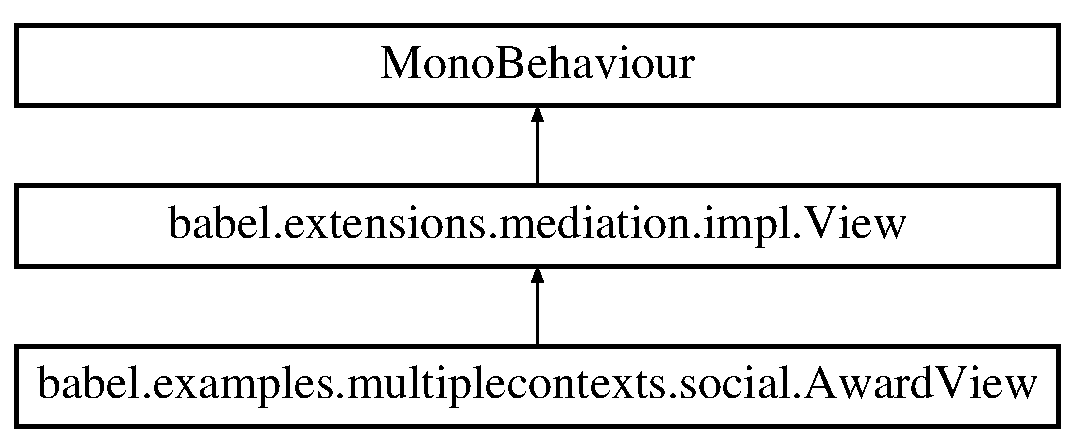
\includegraphics[height=3.000000cm]{classbabel_1_1examples_1_1multiplecontexts_1_1social_1_1_award_view}
\end{center}
\end{figure}
\subsection*{Additional Inherited Members}


The documentation for this class was generated from the following file\-:\begin{DoxyCompactItemize}
\item 
Assets/scripts/babel/examples/multiplecontexts/social/view/Award\-View.\-cs\end{DoxyCompactItemize}

\hypertarget{classbabel_1_1examples_1_1multiplecontexts_1_1social_1_1_award_view_mediator}{\section{babel.\-examples.\-multiplecontexts.\-social.\-Award\-View\-Mediator Class Reference}
\label{classbabel_1_1examples_1_1multiplecontexts_1_1social_1_1_award_view_mediator}\index{babel.\-examples.\-multiplecontexts.\-social.\-Award\-View\-Mediator@{babel.\-examples.\-multiplecontexts.\-social.\-Award\-View\-Mediator}}
}
Inheritance diagram for babel.\-examples.\-multiplecontexts.\-social.\-Award\-View\-Mediator\-:\begin{figure}[H]
\begin{center}
\leavevmode
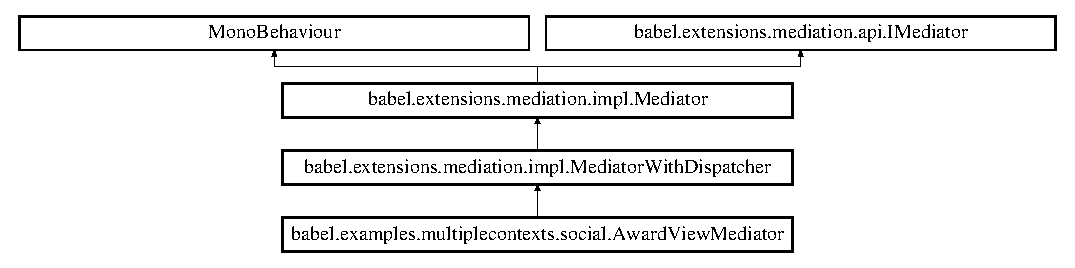
\includegraphics[height=3.154930cm]{classbabel_1_1examples_1_1multiplecontexts_1_1social_1_1_award_view_mediator}
\end{center}
\end{figure}
\subsection*{Public Member Functions}
\begin{DoxyCompactItemize}
\item 
override void \hyperlink{classbabel_1_1examples_1_1multiplecontexts_1_1social_1_1_award_view_mediator_a28e5c49925670e32ccbd82c332b4b5fc}{on\-Register} ()
\begin{DoxyCompactList}\small\item\em Fires after all injections satisifed. \end{DoxyCompactList}\item 
override void \hyperlink{classbabel_1_1examples_1_1multiplecontexts_1_1social_1_1_award_view_mediator_a7571aa44095d692f2c08f589ec4b8bf4}{on\-Remove} ()
\begin{DoxyCompactList}\small\item\em Fires on removal of view. \end{DoxyCompactList}\end{DoxyCompactItemize}
\subsection*{Additional Inherited Members}


\subsection{Member Function Documentation}
\hypertarget{classbabel_1_1examples_1_1multiplecontexts_1_1social_1_1_award_view_mediator_a28e5c49925670e32ccbd82c332b4b5fc}{\index{babel\-::examples\-::multiplecontexts\-::social\-::\-Award\-View\-Mediator@{babel\-::examples\-::multiplecontexts\-::social\-::\-Award\-View\-Mediator}!on\-Register@{on\-Register}}
\index{on\-Register@{on\-Register}!babel::examples::multiplecontexts::social::AwardViewMediator@{babel\-::examples\-::multiplecontexts\-::social\-::\-Award\-View\-Mediator}}
\subsubsection[{on\-Register}]{\setlength{\rightskip}{0pt plus 5cm}override void babel.\-examples.\-multiplecontexts.\-social.\-Award\-View\-Mediator.\-on\-Register (
\begin{DoxyParamCaption}
{}
\end{DoxyParamCaption}
)\hspace{0.3cm}{\ttfamily [inline]}, {\ttfamily [virtual]}}}\label{classbabel_1_1examples_1_1multiplecontexts_1_1social_1_1_award_view_mediator_a28e5c49925670e32ccbd82c332b4b5fc}


Fires after all injections satisifed. 

Override and place your initialization code here. 

Reimplemented from \hyperlink{classbabel_1_1extensions_1_1mediation_1_1impl_1_1_mediator_a693800cf98ef09c660de249436108d9a}{babel.\-extensions.\-mediation.\-impl.\-Mediator}.

\hypertarget{classbabel_1_1examples_1_1multiplecontexts_1_1social_1_1_award_view_mediator_a7571aa44095d692f2c08f589ec4b8bf4}{\index{babel\-::examples\-::multiplecontexts\-::social\-::\-Award\-View\-Mediator@{babel\-::examples\-::multiplecontexts\-::social\-::\-Award\-View\-Mediator}!on\-Remove@{on\-Remove}}
\index{on\-Remove@{on\-Remove}!babel::examples::multiplecontexts::social::AwardViewMediator@{babel\-::examples\-::multiplecontexts\-::social\-::\-Award\-View\-Mediator}}
\subsubsection[{on\-Remove}]{\setlength{\rightskip}{0pt plus 5cm}override void babel.\-examples.\-multiplecontexts.\-social.\-Award\-View\-Mediator.\-on\-Remove (
\begin{DoxyParamCaption}
{}
\end{DoxyParamCaption}
)\hspace{0.3cm}{\ttfamily [inline]}, {\ttfamily [virtual]}}}\label{classbabel_1_1examples_1_1multiplecontexts_1_1social_1_1_award_view_mediator_a7571aa44095d692f2c08f589ec4b8bf4}


Fires on removal of view. 

Override and place your cleanup code here 

Reimplemented from \hyperlink{classbabel_1_1extensions_1_1mediation_1_1impl_1_1_mediator_a8b818665eda883eac66c83b8468007e9}{babel.\-extensions.\-mediation.\-impl.\-Mediator}.



The documentation for this class was generated from the following file\-:\begin{DoxyCompactItemize}
\item 
Assets/scripts/babel/examples/multiplecontexts/social/view/Award\-View\-Mediator.\-cs\end{DoxyCompactItemize}

\hypertarget{class_binder}{\section{Binder Class Reference}
\label{class_binder}\index{Binder@{Binder}}
}


\subsection{Detailed Description}
\begin{DoxySeeAlso}{See Also}
\hyperlink{interfacestrange_1_1framework_1_1api_1_1_i_binder}{strange.\-framework.\-api.\-I\-Binder}. 
\end{DoxySeeAlso}


The documentation for this class was generated from the following file\-:\begin{DoxyCompactItemize}
\item 
Assets/scripts/strange/framework/impl/Binder.\-cs\end{DoxyCompactItemize}

\hypertarget{classbabel_1_1framework_1_1impl_1_1_binding}{\section{babel.\-framework.\-impl.\-Binding Class Reference}
\label{classbabel_1_1framework_1_1impl_1_1_binding}\index{babel.\-framework.\-impl.\-Binding@{babel.\-framework.\-impl.\-Binding}}
}
Inheritance diagram for babel.\-framework.\-impl.\-Binding\-:\begin{figure}[H]
\begin{center}
\leavevmode
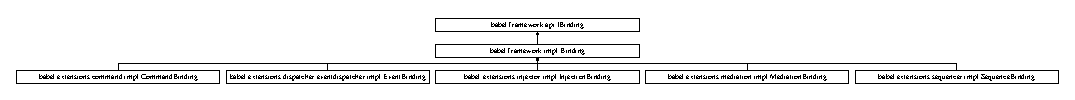
\includegraphics[height=0.896000cm]{classbabel_1_1framework_1_1impl_1_1_binding}
\end{center}
\end{figure}
\subsection*{Public Member Functions}
\begin{DoxyCompactItemize}
\item 
\hypertarget{classbabel_1_1framework_1_1impl_1_1_binding_a626552250ec308ab7dc5a6b00f4b3925}{{\bfseries Binding} (Binder.\-Binding\-Resolver resolver)}\label{classbabel_1_1framework_1_1impl_1_1_binding_a626552250ec308ab7dc5a6b00f4b3925}

\item 
\hypertarget{classbabel_1_1framework_1_1impl_1_1_binding_a74487f5434c66a32bb463a24a995b9d9}{virtual \hyperlink{interfacebabel_1_1framework_1_1api_1_1_i_binding}{I\-Binding} {\bfseries Key$<$ T $>$} ()}\label{classbabel_1_1framework_1_1impl_1_1_binding_a74487f5434c66a32bb463a24a995b9d9}

\item 
\hypertarget{classbabel_1_1framework_1_1impl_1_1_binding_a7044dbf99dea66db4a33749145c8de0b}{virtual \hyperlink{interfacebabel_1_1framework_1_1api_1_1_i_binding}{I\-Binding} {\bfseries Key} (object o)}\label{classbabel_1_1framework_1_1impl_1_1_binding_a7044dbf99dea66db4a33749145c8de0b}

\item 
\hypertarget{classbabel_1_1framework_1_1impl_1_1_binding_aa4ec93fbdff2be0fe36c809770ee55ed}{virtual \hyperlink{interfacebabel_1_1framework_1_1api_1_1_i_binding}{I\-Binding} {\bfseries To$<$ T $>$} ()}\label{classbabel_1_1framework_1_1impl_1_1_binding_aa4ec93fbdff2be0fe36c809770ee55ed}

\item 
\hypertarget{classbabel_1_1framework_1_1impl_1_1_binding_ae4e218eddd9061c76ecc9e8400d50f8b}{virtual \hyperlink{interfacebabel_1_1framework_1_1api_1_1_i_binding}{I\-Binding} {\bfseries To} (object o)}\label{classbabel_1_1framework_1_1impl_1_1_binding_ae4e218eddd9061c76ecc9e8400d50f8b}

\item 
\hypertarget{classbabel_1_1framework_1_1impl_1_1_binding_a75aff3feeb9fdf66e5cf053ca036e834}{virtual \hyperlink{interfacebabel_1_1framework_1_1api_1_1_i_binding}{I\-Binding} {\bfseries To\-Name$<$ T $>$} ()}\label{classbabel_1_1framework_1_1impl_1_1_binding_a75aff3feeb9fdf66e5cf053ca036e834}

\item 
\hypertarget{classbabel_1_1framework_1_1impl_1_1_binding_ac26e26059629c620cfacf7cdac869936}{virtual \hyperlink{interfacebabel_1_1framework_1_1api_1_1_i_binding}{I\-Binding} {\bfseries To\-Name} (object o)}\label{classbabel_1_1framework_1_1impl_1_1_binding_ac26e26059629c620cfacf7cdac869936}

\item 
\hypertarget{classbabel_1_1framework_1_1impl_1_1_binding_a1a9e832af25370e754fc93e67974c4c1}{virtual \hyperlink{interfacebabel_1_1framework_1_1api_1_1_i_binding}{I\-Binding} {\bfseries Named$<$ T $>$} ()}\label{classbabel_1_1framework_1_1impl_1_1_binding_a1a9e832af25370e754fc93e67974c4c1}

\item 
\hypertarget{classbabel_1_1framework_1_1impl_1_1_binding_a02fbdfc3cb6dc671d993a9bbcf26cfaf}{virtual \hyperlink{interfacebabel_1_1framework_1_1api_1_1_i_binding}{I\-Binding} {\bfseries Named} (object o)}\label{classbabel_1_1framework_1_1impl_1_1_binding_a02fbdfc3cb6dc671d993a9bbcf26cfaf}

\item 
\hypertarget{classbabel_1_1framework_1_1impl_1_1_binding_a34f7554d978d2aee46c67f3265b914b9}{virtual void {\bfseries Remove\-Key} (object o)}\label{classbabel_1_1framework_1_1impl_1_1_binding_a34f7554d978d2aee46c67f3265b914b9}

\item 
\hypertarget{classbabel_1_1framework_1_1impl_1_1_binding_ac95bd7154ad91a008297851d7c24f4b8}{virtual void {\bfseries Remove\-Value} (object o)}\label{classbabel_1_1framework_1_1impl_1_1_binding_ac95bd7154ad91a008297851d7c24f4b8}

\item 
\hypertarget{classbabel_1_1framework_1_1impl_1_1_binding_a7e10d84530240f7c066fb998b3b84abb}{virtual void {\bfseries Remove\-Name} (object o)}\label{classbabel_1_1framework_1_1impl_1_1_binding_a7e10d84530240f7c066fb998b3b84abb}

\end{DoxyCompactItemize}
\subsection*{Public Attributes}
\begin{DoxyCompactItemize}
\item 
\hypertarget{classbabel_1_1framework_1_1impl_1_1_binding_a87908d809efd8856c8b01172cfe423e2}{Binder.\-Binding\-Resolver {\bfseries resolver}}\label{classbabel_1_1framework_1_1impl_1_1_binding_a87908d809efd8856c8b01172cfe423e2}

\end{DoxyCompactItemize}
\subsection*{Protected Attributes}
\begin{DoxyCompactItemize}
\item 
\hypertarget{classbabel_1_1framework_1_1impl_1_1_binding_ad5a4fd1dad04b70cc07e860709a0efc5}{\hyperlink{interfacebabel_1_1framework_1_1api_1_1_i_semi_binding}{I\-Semi\-Binding} {\bfseries \-\_\-key}}\label{classbabel_1_1framework_1_1impl_1_1_binding_ad5a4fd1dad04b70cc07e860709a0efc5}

\item 
\hypertarget{classbabel_1_1framework_1_1impl_1_1_binding_a1c5a06d28eee6a10902439dda69fc297}{\hyperlink{interfacebabel_1_1framework_1_1api_1_1_i_semi_binding}{I\-Semi\-Binding} {\bfseries \-\_\-value}}\label{classbabel_1_1framework_1_1impl_1_1_binding_a1c5a06d28eee6a10902439dda69fc297}

\item 
\hypertarget{classbabel_1_1framework_1_1impl_1_1_binding_a7d8e433ce064edb6772c90951d30e87a}{\hyperlink{interfacebabel_1_1framework_1_1api_1_1_i_semi_binding}{I\-Semi\-Binding} {\bfseries \-\_\-name}}\label{classbabel_1_1framework_1_1impl_1_1_binding_a7d8e433ce064edb6772c90951d30e87a}

\end{DoxyCompactItemize}
\subsection*{Properties}
\begin{DoxyCompactItemize}
\item 
\hypertarget{classbabel_1_1framework_1_1impl_1_1_binding_a458cb215336f5aeda7edcd7fdefa9e2c}{object {\bfseries key}\hspace{0.3cm}{\ttfamily  \mbox{[}get\mbox{]}}}\label{classbabel_1_1framework_1_1impl_1_1_binding_a458cb215336f5aeda7edcd7fdefa9e2c}

\item 
\hypertarget{classbabel_1_1framework_1_1impl_1_1_binding_a9a37e8b5b0098334e3d52151938010d8}{object {\bfseries value}\hspace{0.3cm}{\ttfamily  \mbox{[}get\mbox{]}}}\label{classbabel_1_1framework_1_1impl_1_1_binding_a9a37e8b5b0098334e3d52151938010d8}

\item 
\hypertarget{classbabel_1_1framework_1_1impl_1_1_binding_a709db18af8280a835bc54280eb301fd5}{object {\bfseries name}\hspace{0.3cm}{\ttfamily  \mbox{[}get\mbox{]}}}\label{classbabel_1_1framework_1_1impl_1_1_binding_a709db18af8280a835bc54280eb301fd5}

\item 
\hypertarget{classbabel_1_1framework_1_1impl_1_1_binding_adcba2638abf7e5e99c27aa48c88457ac}{Enum {\bfseries key\-Constraint}\hspace{0.3cm}{\ttfamily  \mbox{[}get, set\mbox{]}}}\label{classbabel_1_1framework_1_1impl_1_1_binding_adcba2638abf7e5e99c27aa48c88457ac}

\item 
\hypertarget{classbabel_1_1framework_1_1impl_1_1_binding_a1580c316d12c17075c48cfb3beb94820}{Enum {\bfseries value\-Constraint}\hspace{0.3cm}{\ttfamily  \mbox{[}get, set\mbox{]}}}\label{classbabel_1_1framework_1_1impl_1_1_binding_a1580c316d12c17075c48cfb3beb94820}

\item 
\hypertarget{classbabel_1_1framework_1_1impl_1_1_binding_adfd4b565f60dd5874c267bbf6b22a486}{Enum {\bfseries name\-Constraint}\hspace{0.3cm}{\ttfamily  \mbox{[}get, set\mbox{]}}}\label{classbabel_1_1framework_1_1impl_1_1_binding_adfd4b565f60dd5874c267bbf6b22a486}

\end{DoxyCompactItemize}


The documentation for this class was generated from the following file\-:\begin{DoxyCompactItemize}
\item 
Assets/scripts/babel/framework/impl/Binding.\-cs\end{DoxyCompactItemize}

\hypertarget{classbabel_1_1examples_1_1myfirstproject_1_1_call_web_service_command}{\section{babel.\-examples.\-myfirstproject.\-Call\-Web\-Service\-Command Class Reference}
\label{classbabel_1_1examples_1_1myfirstproject_1_1_call_web_service_command}\index{babel.\-examples.\-myfirstproject.\-Call\-Web\-Service\-Command@{babel.\-examples.\-myfirstproject.\-Call\-Web\-Service\-Command}}
}
Inheritance diagram for babel.\-examples.\-myfirstproject.\-Call\-Web\-Service\-Command\-:\begin{figure}[H]
\begin{center}
\leavevmode
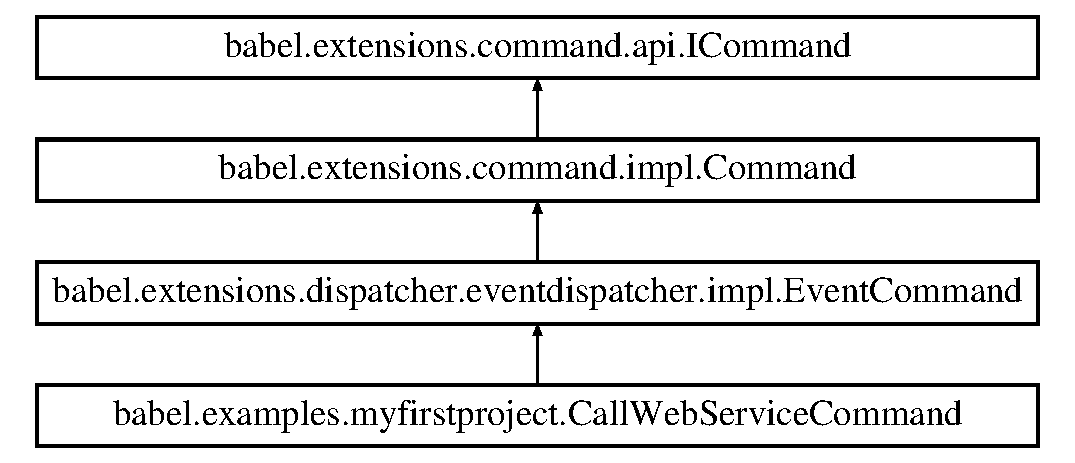
\includegraphics[height=4.000000cm]{classbabel_1_1examples_1_1myfirstproject_1_1_call_web_service_command}
\end{center}
\end{figure}
\subsection*{Public Member Functions}
\begin{DoxyCompactItemize}
\item 
\hypertarget{classbabel_1_1examples_1_1myfirstproject_1_1_call_web_service_command_a26d1a70261d7c93243128056eaa456ae}{override void {\bfseries Execute} ()}\label{classbabel_1_1examples_1_1myfirstproject_1_1_call_web_service_command_a26d1a70261d7c93243128056eaa456ae}

\end{DoxyCompactItemize}
\subsection*{Properties}
\begin{DoxyCompactItemize}
\item 
\hypertarget{classbabel_1_1examples_1_1myfirstproject_1_1_call_web_service_command_a3af55505d6aad9dde6e143797ecd94f2}{\hyperlink{interfacebabel_1_1examples_1_1myfirstproject_1_1_i_example_model}{I\-Example\-Model} {\bfseries model}\hspace{0.3cm}{\ttfamily  \mbox{[}get, set\mbox{]}}}\label{classbabel_1_1examples_1_1myfirstproject_1_1_call_web_service_command_a3af55505d6aad9dde6e143797ecd94f2}

\item 
\hypertarget{classbabel_1_1examples_1_1myfirstproject_1_1_call_web_service_command_adedd153cc219345dcad60cd6109f447d}{\hyperlink{interfacebabel_1_1examples_1_1myfirstproject_1_1_i_example_service}{I\-Example\-Service} {\bfseries service}\hspace{0.3cm}{\ttfamily  \mbox{[}get, set\mbox{]}}}\label{classbabel_1_1examples_1_1myfirstproject_1_1_call_web_service_command_adedd153cc219345dcad60cd6109f447d}

\end{DoxyCompactItemize}


The documentation for this class was generated from the following file\-:\begin{DoxyCompactItemize}
\item 
Assets/scripts/babel/examples/myfirstproject/controller/Call\-Web\-Service\-Command.\-cs\end{DoxyCompactItemize}

\hypertarget{classbabel_1_1examples_1_1multiplecontexts_1_1game_1_1_click_detector}{\section{babel.\-examples.\-multiplecontexts.\-game.\-Click\-Detector Class Reference}
\label{classbabel_1_1examples_1_1multiplecontexts_1_1game_1_1_click_detector}\index{babel.\-examples.\-multiplecontexts.\-game.\-Click\-Detector@{babel.\-examples.\-multiplecontexts.\-game.\-Click\-Detector}}
}
Inheritance diagram for babel.\-examples.\-multiplecontexts.\-game.\-Click\-Detector\-:\begin{figure}[H]
\begin{center}
\leavevmode
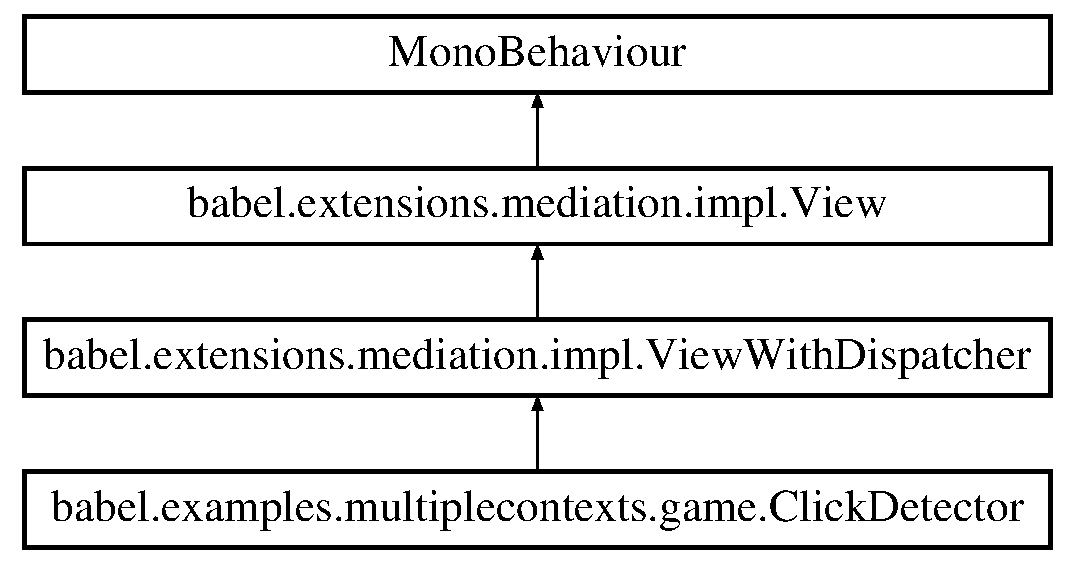
\includegraphics[height=4.000000cm]{classbabel_1_1examples_1_1multiplecontexts_1_1game_1_1_click_detector}
\end{center}
\end{figure}
\subsection*{Public Attributes}
\begin{DoxyCompactItemize}
\item 
\hypertarget{classbabel_1_1examples_1_1multiplecontexts_1_1game_1_1_click_detector_a821762a5d3eecab4e2daa35ddae55f1c}{const string {\bfseries C\-L\-I\-C\-K} = \char`\"{}C\-L\-I\-C\-K\char`\"{}}\label{classbabel_1_1examples_1_1multiplecontexts_1_1game_1_1_click_detector_a821762a5d3eecab4e2daa35ddae55f1c}

\end{DoxyCompactItemize}
\subsection*{Additional Inherited Members}


The documentation for this class was generated from the following file\-:\begin{DoxyCompactItemize}
\item 
Assets/scripts/babel/examples/multiplecontexts/game/view/Click\-Detector.\-cs\end{DoxyCompactItemize}

\hypertarget{classbabel_1_1examples_1_1myfirstproject_1_1_click_detector}{\section{babel.\-examples.\-myfirstproject.\-Click\-Detector Class Reference}
\label{classbabel_1_1examples_1_1myfirstproject_1_1_click_detector}\index{babel.\-examples.\-myfirstproject.\-Click\-Detector@{babel.\-examples.\-myfirstproject.\-Click\-Detector}}
}
Inheritance diagram for babel.\-examples.\-myfirstproject.\-Click\-Detector\-:\begin{figure}[H]
\begin{center}
\leavevmode
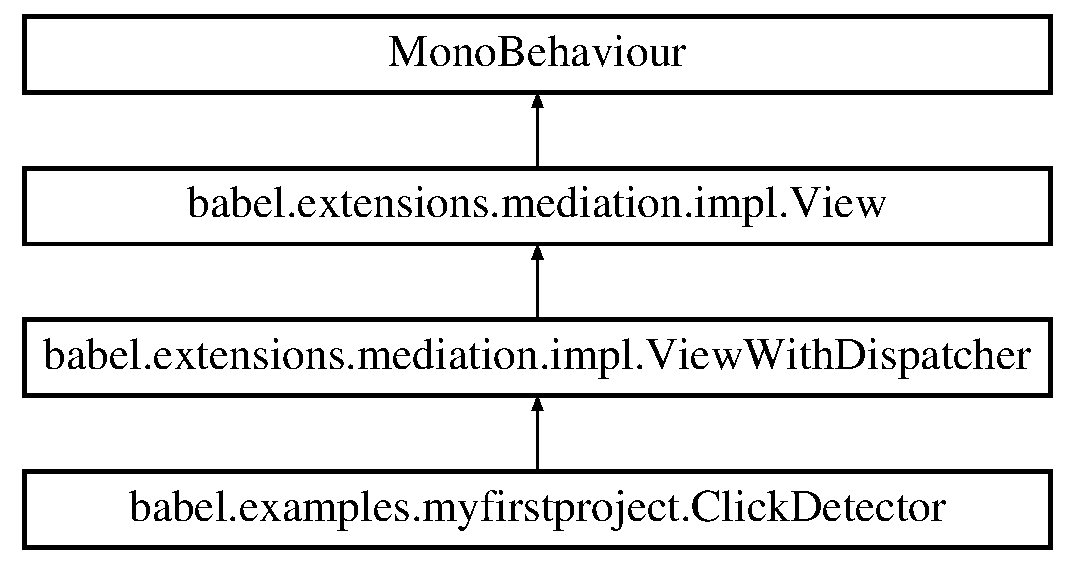
\includegraphics[height=4.000000cm]{classbabel_1_1examples_1_1myfirstproject_1_1_click_detector}
\end{center}
\end{figure}
\subsection*{Public Attributes}
\begin{DoxyCompactItemize}
\item 
\hypertarget{classbabel_1_1examples_1_1myfirstproject_1_1_click_detector_a8005d0675a4d6caf5a30205e6414f3a1}{const string {\bfseries C\-L\-I\-C\-K} = \char`\"{}C\-L\-I\-C\-K\char`\"{}}\label{classbabel_1_1examples_1_1myfirstproject_1_1_click_detector_a8005d0675a4d6caf5a30205e6414f3a1}

\end{DoxyCompactItemize}
\subsection*{Additional Inherited Members}


The documentation for this class was generated from the following file\-:\begin{DoxyCompactItemize}
\item 
Assets/scripts/babel/examples/myfirstproject/view/Click\-Detector.\-cs\end{DoxyCompactItemize}

\hypertarget{classbabel_1_1extensions_1_1command_1_1impl_1_1_command}{\section{babel.\-extensions.\-command.\-impl.\-Command Class Reference}
\label{classbabel_1_1extensions_1_1command_1_1impl_1_1_command}\index{babel.\-extensions.\-command.\-impl.\-Command@{babel.\-extensions.\-command.\-impl.\-Command}}
}
Inheritance diagram for babel.\-extensions.\-command.\-impl.\-Command\-:\begin{figure}[H]
\begin{center}
\leavevmode
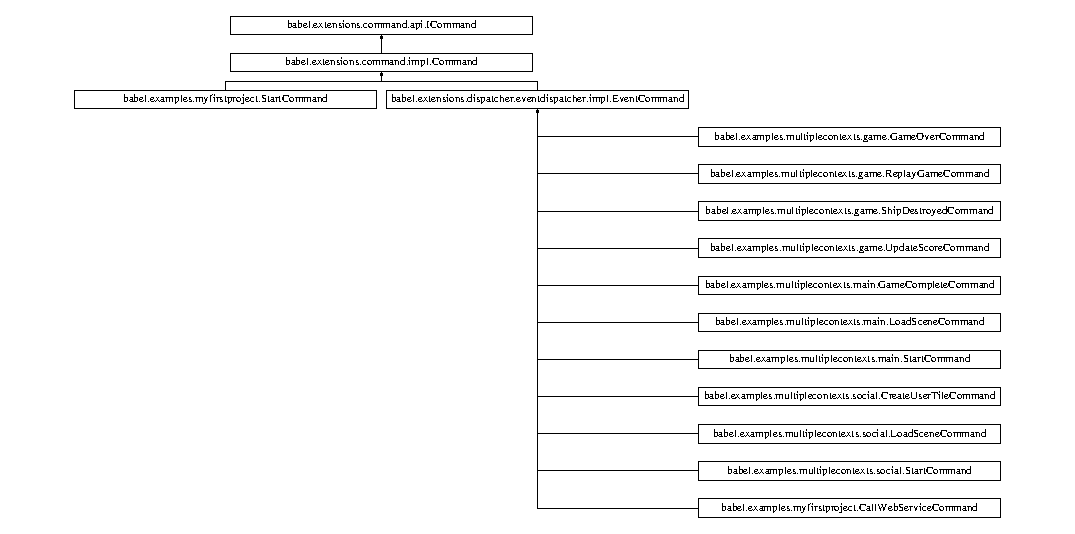
\includegraphics[height=6.735395cm]{classbabel_1_1extensions_1_1command_1_1impl_1_1_command}
\end{center}
\end{figure}
\subsection*{Public Member Functions}
\begin{DoxyCompactItemize}
\item 
\hypertarget{classbabel_1_1extensions_1_1command_1_1impl_1_1_command_a18329c34d3b0815f1196c4d68fce90e8}{virtual void {\bfseries Execute} ()}\label{classbabel_1_1extensions_1_1command_1_1impl_1_1_command_a18329c34d3b0815f1196c4d68fce90e8}

\item 
\hypertarget{classbabel_1_1extensions_1_1command_1_1impl_1_1_command_aa90a93a40f905804f3ada35ff0aab064}{void {\bfseries Retain} ()}\label{classbabel_1_1extensions_1_1command_1_1impl_1_1_command_aa90a93a40f905804f3ada35ff0aab064}

\item 
\hypertarget{classbabel_1_1extensions_1_1command_1_1impl_1_1_command_a66863c2282a97a3c4b6863bce595485f}{void {\bfseries Release} ()}\label{classbabel_1_1extensions_1_1command_1_1impl_1_1_command_a66863c2282a97a3c4b6863bce595485f}

\item 
\hypertarget{classbabel_1_1extensions_1_1command_1_1impl_1_1_command_aab75ab7a182f404a4d399d38876dbbaa}{virtual void {\bfseries Dispose} ()}\label{classbabel_1_1extensions_1_1command_1_1impl_1_1_command_aab75ab7a182f404a4d399d38876dbbaa}

\end{DoxyCompactItemize}
\subsection*{Properties}
\begin{DoxyCompactItemize}
\item 
\hypertarget{classbabel_1_1extensions_1_1command_1_1impl_1_1_command_a45523839d897d6b240c8884e83aea629}{\hyperlink{interfacebabel_1_1extensions_1_1command_1_1api_1_1_i_command_binder}{I\-Command\-Binder} {\bfseries command\-Binder}\hspace{0.3cm}{\ttfamily  \mbox{[}get, set\mbox{]}}}\label{classbabel_1_1extensions_1_1command_1_1impl_1_1_command_a45523839d897d6b240c8884e83aea629}

\item 
\hypertarget{classbabel_1_1extensions_1_1command_1_1impl_1_1_command_aa26d05de61b3d7eb425e71bab882c544}{\hyperlink{interfacebabel_1_1extensions_1_1injector_1_1api_1_1_i_injection_binder}{I\-Injection\-Binder} {\bfseries injection\-Binder}\hspace{0.3cm}{\ttfamily  \mbox{[}get, set\mbox{]}}}\label{classbabel_1_1extensions_1_1command_1_1impl_1_1_command_aa26d05de61b3d7eb425e71bab882c544}

\item 
\hypertarget{classbabel_1_1extensions_1_1command_1_1impl_1_1_command_a0beb2f432887b83961bd6a504d27face}{object {\bfseries data}\hspace{0.3cm}{\ttfamily  \mbox{[}get, set\mbox{]}}}\label{classbabel_1_1extensions_1_1command_1_1impl_1_1_command_a0beb2f432887b83961bd6a504d27face}

\item 
\hypertarget{classbabel_1_1extensions_1_1command_1_1impl_1_1_command_ae73973077ae842836f017a489f8bdcb1}{bool {\bfseries retain}\hspace{0.3cm}{\ttfamily  \mbox{[}get\mbox{]}}}\label{classbabel_1_1extensions_1_1command_1_1impl_1_1_command_ae73973077ae842836f017a489f8bdcb1}

\end{DoxyCompactItemize}


The documentation for this class was generated from the following file\-:\begin{DoxyCompactItemize}
\item 
Assets/scripts/babel/extensions/command/impl/Command.\-cs\end{DoxyCompactItemize}

\hypertarget{classbabel_1_1extensions_1_1command_1_1impl_1_1_command_binder}{\section{babel.\-extensions.\-command.\-impl.\-Command\-Binder Class Reference}
\label{classbabel_1_1extensions_1_1command_1_1impl_1_1_command_binder}\index{babel.\-extensions.\-command.\-impl.\-Command\-Binder@{babel.\-extensions.\-command.\-impl.\-Command\-Binder}}
}
Inheritance diagram for babel.\-extensions.\-command.\-impl.\-Command\-Binder\-:\begin{figure}[H]
\begin{center}
\leavevmode
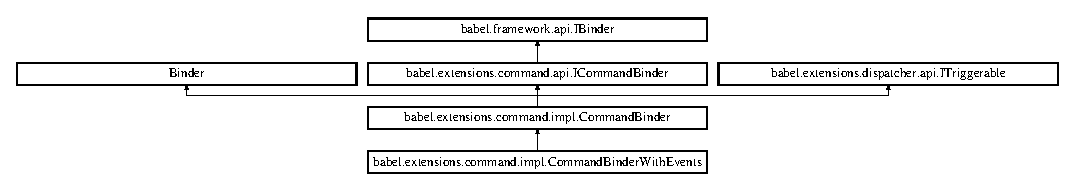
\includegraphics[height=2.103286cm]{classbabel_1_1extensions_1_1command_1_1impl_1_1_command_binder}
\end{center}
\end{figure}
\subsection*{Public Member Functions}
\begin{DoxyCompactItemize}
\item 
\hypertarget{classbabel_1_1extensions_1_1command_1_1impl_1_1_command_binder_a979753b42f167f16ae39f178296ee909}{override \hyperlink{interfacebabel_1_1framework_1_1api_1_1_i_binding}{I\-Binding} {\bfseries Get\-Raw\-Binding} ()}\label{classbabel_1_1extensions_1_1command_1_1impl_1_1_command_binder_a979753b42f167f16ae39f178296ee909}

\item 
void \hyperlink{classbabel_1_1extensions_1_1command_1_1impl_1_1_command_binder_a9d286dbf28eb4b1ebf7e2c45b8a74d21}{React\-To} (object trigger)
\begin{DoxyCompactList}\small\item\em Instantiate and execute one or more Commands based on the input. \end{DoxyCompactList}\item 
\hypertarget{classbabel_1_1extensions_1_1command_1_1impl_1_1_command_binder_adf768bc0eafab66e8bd87a75b8b44804}{void {\bfseries React\-To} (object trigger, object data)}\label{classbabel_1_1extensions_1_1command_1_1impl_1_1_command_binder_adf768bc0eafab66e8bd87a75b8b44804}

\item 
void \hyperlink{classbabel_1_1extensions_1_1command_1_1impl_1_1_command_binder_a5f254fbeda04e19eabdd104458210087}{Release\-Command} (\hyperlink{interfacebabel_1_1extensions_1_1command_1_1api_1_1_i_command}{I\-Command} command)
\begin{DoxyCompactList}\small\item\em Release a previously retained \hyperlink{classbabel_1_1extensions_1_1command_1_1impl_1_1_command}{Command}. \end{DoxyCompactList}\item 
\hypertarget{classbabel_1_1extensions_1_1command_1_1impl_1_1_command_binder_a28178b4899ba1f1e874cd2e87b9c5362}{void {\bfseries Trigger$<$ T $>$} (object data)}\label{classbabel_1_1extensions_1_1command_1_1impl_1_1_command_binder_a28178b4899ba1f1e874cd2e87b9c5362}

\item 
\hypertarget{classbabel_1_1extensions_1_1command_1_1impl_1_1_command_binder_a0f5f258056155eaf04c16b8dfb00bcdb}{void {\bfseries Trigger} (object key, object data)}\label{classbabel_1_1extensions_1_1command_1_1impl_1_1_command_binder_a0f5f258056155eaf04c16b8dfb00bcdb}

\item 
\hypertarget{classbabel_1_1extensions_1_1command_1_1impl_1_1_command_binder_a0b332603307578e797d407434be99c1e}{new \hyperlink{interfacebabel_1_1extensions_1_1command_1_1api_1_1_i_command_binding}{I\-Command\-Binding} {\bfseries Bind$<$ T $>$} ()}\label{classbabel_1_1extensions_1_1command_1_1impl_1_1_command_binder_a0b332603307578e797d407434be99c1e}

\item 
\hypertarget{classbabel_1_1extensions_1_1command_1_1impl_1_1_command_binder_a2663eb8285249630cf16d835a9cc6720}{new \hyperlink{interfacebabel_1_1extensions_1_1command_1_1api_1_1_i_command_binding}{I\-Command\-Binding} {\bfseries Bind} (object value)}\label{classbabel_1_1extensions_1_1command_1_1impl_1_1_command_binder_a2663eb8285249630cf16d835a9cc6720}

\end{DoxyCompactItemize}
\subsection*{Protected Member Functions}
\begin{DoxyCompactItemize}
\item 
\hypertarget{classbabel_1_1extensions_1_1command_1_1impl_1_1_command_binder_a000a53453bcd9e119e3d24a73f60383f}{virtual void {\bfseries invoke\-Command} (Type cmd, \hyperlink{interfacebabel_1_1extensions_1_1command_1_1api_1_1_i_command_binding}{I\-Command\-Binding} binding, object data, int depth)}\label{classbabel_1_1extensions_1_1command_1_1impl_1_1_command_binder_a000a53453bcd9e119e3d24a73f60383f}

\item 
\hypertarget{classbabel_1_1extensions_1_1command_1_1impl_1_1_command_binder_a7776192269f851a72ef26a4ffee2c03b}{virtual \hyperlink{interfacebabel_1_1extensions_1_1command_1_1api_1_1_i_command}{I\-Command} {\bfseries create\-Command} (object cmd, object data)}\label{classbabel_1_1extensions_1_1command_1_1impl_1_1_command_binder_a7776192269f851a72ef26a4ffee2c03b}

\end{DoxyCompactItemize}
\subsection*{Protected Attributes}
\begin{DoxyCompactItemize}
\item 
\hypertarget{classbabel_1_1extensions_1_1command_1_1impl_1_1_command_binder_af97f8495f075cb96ff71c0a6db7dfb27}{Dictionary$<$ \hyperlink{interfacebabel_1_1extensions_1_1command_1_1api_1_1_i_command}{I\-Command}, \hyperlink{interfacebabel_1_1extensions_1_1command_1_1api_1_1_i_command}{I\-Command} $>$ {\bfseries active\-Commands} = new Dictionary$<$\hyperlink{interfacebabel_1_1extensions_1_1command_1_1api_1_1_i_command}{I\-Command}, \hyperlink{interfacebabel_1_1extensions_1_1command_1_1api_1_1_i_command}{I\-Command}$>$()}\label{classbabel_1_1extensions_1_1command_1_1impl_1_1_command_binder_af97f8495f075cb96ff71c0a6db7dfb27}

\end{DoxyCompactItemize}
\subsection*{Properties}
\begin{DoxyCompactItemize}
\item 
\hypertarget{classbabel_1_1extensions_1_1command_1_1impl_1_1_command_binder_a83fce533afb137bf0e3a0e6e3d946e19}{\hyperlink{interfacebabel_1_1extensions_1_1injector_1_1api_1_1_i_injection_binder}{I\-Injection\-Binder} {\bfseries injection\-Binder}\hspace{0.3cm}{\ttfamily  \mbox{[}get, set\mbox{]}}}\label{classbabel_1_1extensions_1_1command_1_1impl_1_1_command_binder_a83fce533afb137bf0e3a0e6e3d946e19}

\end{DoxyCompactItemize}


\subsection{Member Function Documentation}
\hypertarget{classbabel_1_1extensions_1_1command_1_1impl_1_1_command_binder_a9d286dbf28eb4b1ebf7e2c45b8a74d21}{\index{babel\-::extensions\-::command\-::impl\-::\-Command\-Binder@{babel\-::extensions\-::command\-::impl\-::\-Command\-Binder}!React\-To@{React\-To}}
\index{React\-To@{React\-To}!babel::extensions::command::impl::CommandBinder@{babel\-::extensions\-::command\-::impl\-::\-Command\-Binder}}
\subsubsection[{React\-To}]{\setlength{\rightskip}{0pt plus 5cm}void babel.\-extensions.\-command.\-impl.\-Command\-Binder.\-React\-To (
\begin{DoxyParamCaption}
\item[{object}]{trigger}
\end{DoxyParamCaption}
)\hspace{0.3cm}{\ttfamily [inline]}}}\label{classbabel_1_1extensions_1_1command_1_1impl_1_1_command_binder_a9d286dbf28eb4b1ebf7e2c45b8a74d21}


Instantiate and execute one or more Commands based on the input. 


\begin{DoxyParams}{Parameters}
{\em trigger} & The key that unlocks the Command(s) \\
\hline
\end{DoxyParams}


Implements \hyperlink{interfacebabel_1_1extensions_1_1command_1_1api_1_1_i_command_binder_a50e05144d88aa86e46b8d78125667e43}{babel.\-extensions.\-command.\-api.\-I\-Command\-Binder}.

\hypertarget{classbabel_1_1extensions_1_1command_1_1impl_1_1_command_binder_a5f254fbeda04e19eabdd104458210087}{\index{babel\-::extensions\-::command\-::impl\-::\-Command\-Binder@{babel\-::extensions\-::command\-::impl\-::\-Command\-Binder}!Release\-Command@{Release\-Command}}
\index{Release\-Command@{Release\-Command}!babel::extensions::command::impl::CommandBinder@{babel\-::extensions\-::command\-::impl\-::\-Command\-Binder}}
\subsubsection[{Release\-Command}]{\setlength{\rightskip}{0pt plus 5cm}void babel.\-extensions.\-command.\-impl.\-Command\-Binder.\-Release\-Command (
\begin{DoxyParamCaption}
\item[{{\bf I\-Command}}]{command}
\end{DoxyParamCaption}
)\hspace{0.3cm}{\ttfamily [inline]}}}\label{classbabel_1_1extensions_1_1command_1_1impl_1_1_command_binder_a5f254fbeda04e19eabdd104458210087}


Release a previously retained \hyperlink{classbabel_1_1extensions_1_1command_1_1impl_1_1_command}{Command}. 

By default, a \hyperlink{classbabel_1_1extensions_1_1command_1_1impl_1_1_command}{Command} is garbage collected at the end of its Execute method. But the \hyperlink{classbabel_1_1extensions_1_1command_1_1impl_1_1_command}{Command} can be retained for asynchronous calls.


\begin{DoxyParams}{Parameters}
{\em The} & \hyperlink{classbabel_1_1extensions_1_1command_1_1impl_1_1_command}{Command} to release \\
\hline
\end{DoxyParams}


Implements \hyperlink{interfacebabel_1_1extensions_1_1command_1_1api_1_1_i_command_binder_a03df21f7c6b2c9628dc00afc34d08a2e}{babel.\-extensions.\-command.\-api.\-I\-Command\-Binder}.



The documentation for this class was generated from the following file\-:\begin{DoxyCompactItemize}
\item 
Assets/scripts/babel/extensions/command/impl/Command\-Binder.\-cs\end{DoxyCompactItemize}

\hypertarget{classbabel_1_1extensions_1_1command_1_1impl_1_1_command_binder_with_events}{\section{babel.\-extensions.\-command.\-impl.\-Command\-Binder\-With\-Events Class Reference}
\label{classbabel_1_1extensions_1_1command_1_1impl_1_1_command_binder_with_events}\index{babel.\-extensions.\-command.\-impl.\-Command\-Binder\-With\-Events@{babel.\-extensions.\-command.\-impl.\-Command\-Binder\-With\-Events}}
}
Inheritance diagram for babel.\-extensions.\-command.\-impl.\-Command\-Binder\-With\-Events\-:\begin{figure}[H]
\begin{center}
\leavevmode
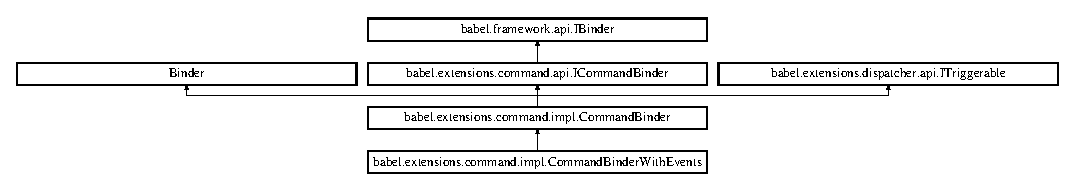
\includegraphics[height=2.103286cm]{classbabel_1_1extensions_1_1command_1_1impl_1_1_command_binder_with_events}
\end{center}
\end{figure}
\subsection*{Protected Member Functions}
\begin{DoxyCompactItemize}
\item 
\hypertarget{classbabel_1_1extensions_1_1command_1_1impl_1_1_command_binder_with_events_a6738d6d2ea289b007adc65aa23378ac2}{override \hyperlink{interfacebabel_1_1extensions_1_1command_1_1api_1_1_i_command}{I\-Command} {\bfseries create\-Command} (object cmd, object data)}\label{classbabel_1_1extensions_1_1command_1_1impl_1_1_command_binder_with_events_a6738d6d2ea289b007adc65aa23378ac2}

\end{DoxyCompactItemize}
\subsection*{Additional Inherited Members}


The documentation for this class was generated from the following file\-:\begin{DoxyCompactItemize}
\item 
Assets/scripts/babel/extensions/command/impl/Command\-Binder\-With\-Events.\-cs\end{DoxyCompactItemize}

\hypertarget{classbabel_1_1extensions_1_1command_1_1impl_1_1_command_binding}{\section{babel.\-extensions.\-command.\-impl.\-Command\-Binding Class Reference}
\label{classbabel_1_1extensions_1_1command_1_1impl_1_1_command_binding}\index{babel.\-extensions.\-command.\-impl.\-Command\-Binding@{babel.\-extensions.\-command.\-impl.\-Command\-Binding}}
}
Inheritance diagram for babel.\-extensions.\-command.\-impl.\-Command\-Binding\-:\begin{figure}[H]
\begin{center}
\leavevmode
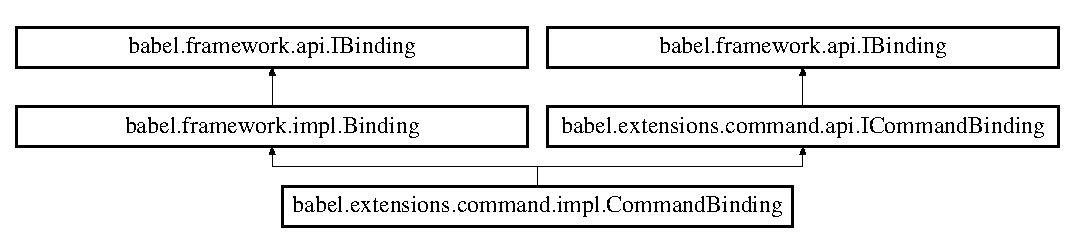
\includegraphics[height=2.818792cm]{classbabel_1_1extensions_1_1command_1_1impl_1_1_command_binding}
\end{center}
\end{figure}
\subsection*{Public Member Functions}
\begin{DoxyCompactItemize}
\item 
\hypertarget{classbabel_1_1extensions_1_1command_1_1impl_1_1_command_binding_a00affc8c84069d1fe32cc01a429c7818}{{\bfseries Command\-Binding} (Binder.\-Binding\-Resolver resolver)}\label{classbabel_1_1extensions_1_1command_1_1impl_1_1_command_binding_a00affc8c84069d1fe32cc01a429c7818}

\item 
\hypertarget{classbabel_1_1extensions_1_1command_1_1impl_1_1_command_binding_ab644d770ab9ee0d4e1bd4df8a16be7af}{\hyperlink{interfacebabel_1_1extensions_1_1command_1_1api_1_1_i_command_binding}{I\-Command\-Binding} {\bfseries Once} ()}\label{classbabel_1_1extensions_1_1command_1_1impl_1_1_command_binding_ab644d770ab9ee0d4e1bd4df8a16be7af}

\item 
\hypertarget{classbabel_1_1extensions_1_1command_1_1impl_1_1_command_binding_a628516f9da2183bfedb503b3726bc366}{\hyperlink{interfacebabel_1_1extensions_1_1command_1_1api_1_1_i_command_binding}{I\-Command\-Binding} {\bfseries Bind$<$ T $>$} ()}\label{classbabel_1_1extensions_1_1command_1_1impl_1_1_command_binding_a628516f9da2183bfedb503b3726bc366}

\item 
\hypertarget{classbabel_1_1extensions_1_1command_1_1impl_1_1_command_binding_a9d32853c984092a07efaabf50a8368f2}{\hyperlink{interfacebabel_1_1extensions_1_1command_1_1api_1_1_i_command_binding}{I\-Command\-Binding} {\bfseries Bind} (object key)}\label{classbabel_1_1extensions_1_1command_1_1impl_1_1_command_binding_a9d32853c984092a07efaabf50a8368f2}

\item 
\hypertarget{classbabel_1_1extensions_1_1command_1_1impl_1_1_command_binding_adb66366cf08228d843afbc9a0706b636}{new \hyperlink{interfacebabel_1_1extensions_1_1command_1_1api_1_1_i_command_binding}{I\-Command\-Binding} \hyperlink{classbabel_1_1extensions_1_1command_1_1impl_1_1_command_binding_adb66366cf08228d843afbc9a0706b636}{Key$<$ T $>$} ()}\label{classbabel_1_1extensions_1_1command_1_1impl_1_1_command_binding_adb66366cf08228d843afbc9a0706b636}

\begin{DoxyCompactList}\small\item\em Below this point is facade for I\-Binding. \end{DoxyCompactList}\item 
\hypertarget{classbabel_1_1extensions_1_1command_1_1impl_1_1_command_binding_a1898b39c5d65fbcbddb7d6f0615001d2}{new \hyperlink{interfacebabel_1_1extensions_1_1command_1_1api_1_1_i_command_binding}{I\-Command\-Binding} {\bfseries Key} (object key)}\label{classbabel_1_1extensions_1_1command_1_1impl_1_1_command_binding_a1898b39c5d65fbcbddb7d6f0615001d2}

\item 
\hypertarget{classbabel_1_1extensions_1_1command_1_1impl_1_1_command_binding_a032509750447b110ed44c2a0e7cb49ca}{new \hyperlink{interfacebabel_1_1extensions_1_1command_1_1api_1_1_i_command_binding}{I\-Command\-Binding} {\bfseries To$<$ T $>$} ()}\label{classbabel_1_1extensions_1_1command_1_1impl_1_1_command_binding_a032509750447b110ed44c2a0e7cb49ca}

\item 
\hypertarget{classbabel_1_1extensions_1_1command_1_1impl_1_1_command_binding_a1ae3f6c6d32d3645da5e55c347344cbd}{new \hyperlink{interfacebabel_1_1extensions_1_1command_1_1api_1_1_i_command_binding}{I\-Command\-Binding} {\bfseries To} (object o)}\label{classbabel_1_1extensions_1_1command_1_1impl_1_1_command_binding_a1ae3f6c6d32d3645da5e55c347344cbd}

\item 
\hypertarget{classbabel_1_1extensions_1_1command_1_1impl_1_1_command_binding_a920878100e86607d1d4291a48640ac96}{new \hyperlink{interfacebabel_1_1extensions_1_1command_1_1api_1_1_i_command_binding}{I\-Command\-Binding} {\bfseries To\-Name$<$ T $>$} ()}\label{classbabel_1_1extensions_1_1command_1_1impl_1_1_command_binding_a920878100e86607d1d4291a48640ac96}

\item 
\hypertarget{classbabel_1_1extensions_1_1command_1_1impl_1_1_command_binding_a2c6e26f56500ea920bac3f9a0451ff64}{new \hyperlink{interfacebabel_1_1extensions_1_1command_1_1api_1_1_i_command_binding}{I\-Command\-Binding} {\bfseries To\-Name} (object o)}\label{classbabel_1_1extensions_1_1command_1_1impl_1_1_command_binding_a2c6e26f56500ea920bac3f9a0451ff64}

\item 
\hypertarget{classbabel_1_1extensions_1_1command_1_1impl_1_1_command_binding_a81417621452edf1ac4f0a93e955755f0}{new \hyperlink{interfacebabel_1_1extensions_1_1command_1_1api_1_1_i_command_binding}{I\-Command\-Binding} {\bfseries Named$<$ T $>$} ()}\label{classbabel_1_1extensions_1_1command_1_1impl_1_1_command_binding_a81417621452edf1ac4f0a93e955755f0}

\item 
\hypertarget{classbabel_1_1extensions_1_1command_1_1impl_1_1_command_binding_a793c2868a93c666ee5891733373f55e1}{new \hyperlink{interfacebabel_1_1extensions_1_1command_1_1api_1_1_i_command_binding}{I\-Command\-Binding} {\bfseries Named} (object o)}\label{classbabel_1_1extensions_1_1command_1_1impl_1_1_command_binding_a793c2868a93c666ee5891733373f55e1}

\end{DoxyCompactItemize}
\subsection*{Properties}
\begin{DoxyCompactItemize}
\item 
\hypertarget{classbabel_1_1extensions_1_1command_1_1impl_1_1_command_binding_aa6de3801a1dff99bf64850b71ef691c0}{bool {\bfseries is\-One\-Off}\hspace{0.3cm}{\ttfamily  \mbox{[}get, set\mbox{]}}}\label{classbabel_1_1extensions_1_1command_1_1impl_1_1_command_binding_aa6de3801a1dff99bf64850b71ef691c0}

\end{DoxyCompactItemize}
\subsection*{Additional Inherited Members}


The documentation for this class was generated from the following file\-:\begin{DoxyCompactItemize}
\item 
Assets/scripts/babel/extensions/command/impl/Command\-Binding.\-cs\end{DoxyCompactItemize}

\hypertarget{classbabel_1_1extensions_1_1command_1_1impl_1_1_command_exception}{\section{babel.\-extensions.\-command.\-impl.\-Command\-Exception Class Reference}
\label{classbabel_1_1extensions_1_1command_1_1impl_1_1_command_exception}\index{babel.\-extensions.\-command.\-impl.\-Command\-Exception@{babel.\-extensions.\-command.\-impl.\-Command\-Exception}}
}
Inheritance diagram for babel.\-extensions.\-command.\-impl.\-Command\-Exception\-:\begin{figure}[H]
\begin{center}
\leavevmode
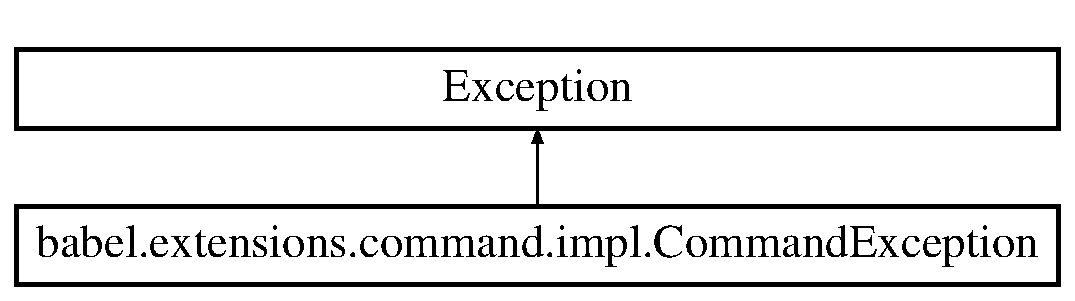
\includegraphics[height=2.000000cm]{classbabel_1_1extensions_1_1command_1_1impl_1_1_command_exception}
\end{center}
\end{figure}
\subsection*{Public Member Functions}
\begin{DoxyCompactItemize}
\item 
\hypertarget{classbabel_1_1extensions_1_1command_1_1impl_1_1_command_exception_ac40ea9765a0c63a59a46a114320602ff}{{\bfseries Command\-Exception} (string message, Command\-Exception\-Type exception\-Type)}\label{classbabel_1_1extensions_1_1command_1_1impl_1_1_command_exception_ac40ea9765a0c63a59a46a114320602ff}

\end{DoxyCompactItemize}
\subsection*{Properties}
\begin{DoxyCompactItemize}
\item 
\hypertarget{classbabel_1_1extensions_1_1command_1_1impl_1_1_command_exception_a8c1e7b89bb7c2d1295c0ab8c980bf139}{Command\-Exception\-Type {\bfseries type}\hspace{0.3cm}{\ttfamily  \mbox{[}get, set\mbox{]}}}\label{classbabel_1_1extensions_1_1command_1_1impl_1_1_command_exception_a8c1e7b89bb7c2d1295c0ab8c980bf139}

\end{DoxyCompactItemize}


The documentation for this class was generated from the following file\-:\begin{DoxyCompactItemize}
\item 
Assets/scripts/babel/extensions/command/impl/Command\-Exception.\-cs\end{DoxyCompactItemize}

\hypertarget{class_construct}{\section{Construct Class Reference}
\label{class_construct}\index{Construct@{Construct}}
}
Inheritance diagram for Construct\-:\begin{figure}[H]
\begin{center}
\leavevmode
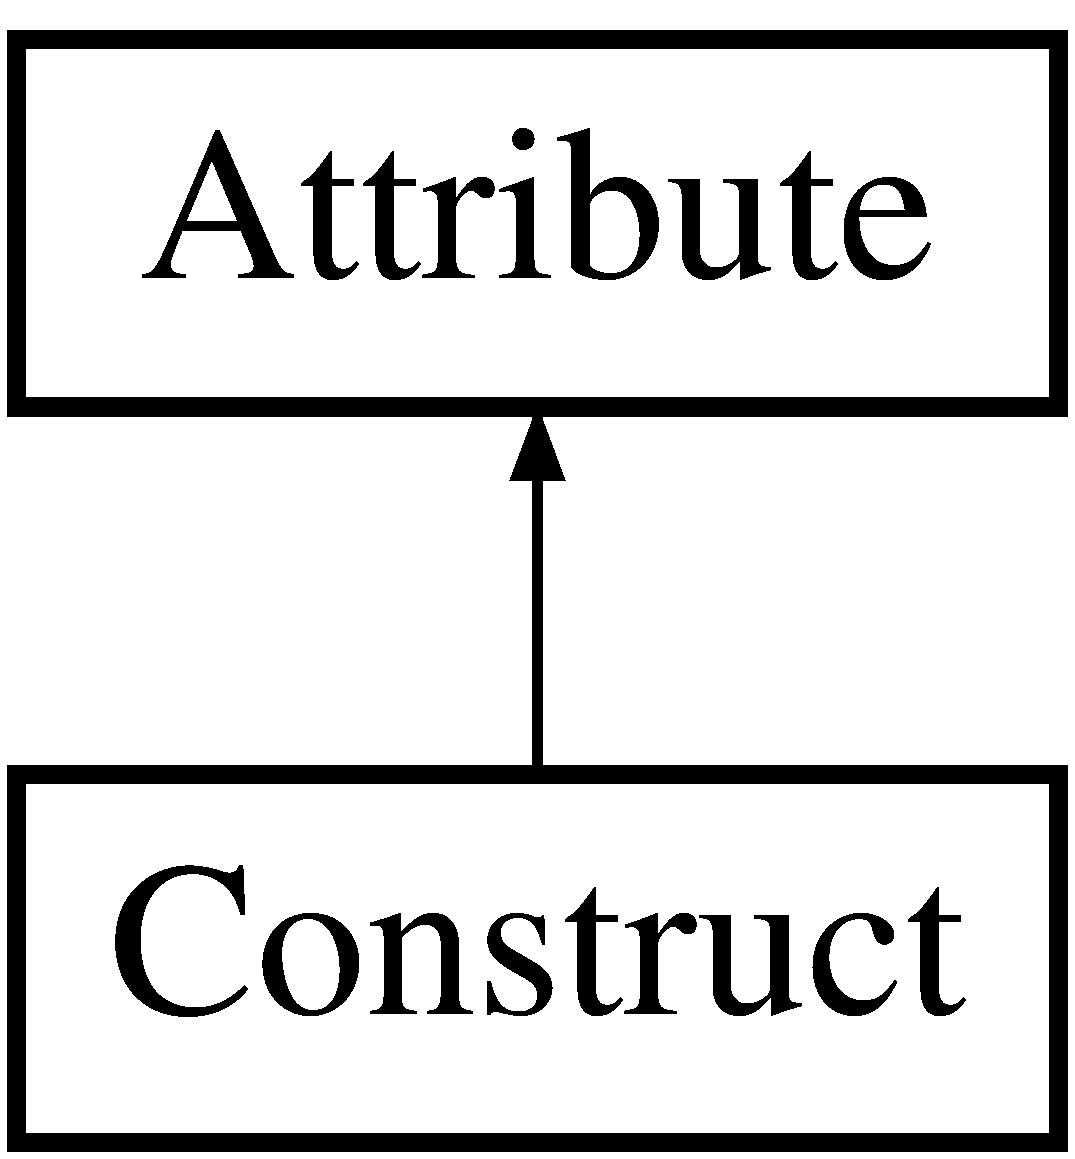
\includegraphics[height=2.000000cm]{class_construct}
\end{center}
\end{figure}


The documentation for this class was generated from the following file\-:\begin{DoxyCompactItemize}
\item 
Assets/scripts/babel/extensions/injector/Inject\-Attribute.\-cs\end{DoxyCompactItemize}

\hypertarget{classbabel_1_1extensions_1_1context_1_1impl_1_1_context}{\section{babel.\-extensions.\-context.\-impl.\-Context Class Reference}
\label{classbabel_1_1extensions_1_1context_1_1impl_1_1_context}\index{babel.\-extensions.\-context.\-impl.\-Context@{babel.\-extensions.\-context.\-impl.\-Context}}
}
Inheritance diagram for babel.\-extensions.\-context.\-impl.\-Context\-:\begin{figure}[H]
\begin{center}
\leavevmode
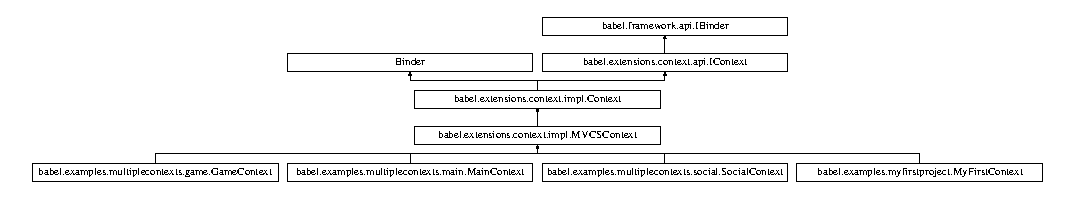
\includegraphics[height=2.208202cm]{classbabel_1_1extensions_1_1context_1_1impl_1_1_context}
\end{center}
\end{figure}
\subsection*{Public Member Functions}
\begin{DoxyCompactItemize}
\item 
\hypertarget{classbabel_1_1extensions_1_1context_1_1impl_1_1_context_ac1f9ee2f2acfcc1915209f9c0b0a13fc}{{\bfseries Context} (object view, bool auto\-Startup)}\label{classbabel_1_1extensions_1_1context_1_1impl_1_1_context_ac1f9ee2f2acfcc1915209f9c0b0a13fc}

\item 
\hypertarget{classbabel_1_1extensions_1_1context_1_1impl_1_1_context_a07e5a15872b32d8736b2209ebfc855be}{virtual \hyperlink{interfacebabel_1_1extensions_1_1context_1_1api_1_1_i_context}{I\-Context} {\bfseries Set\-Context\-View} (object view)}\label{classbabel_1_1extensions_1_1context_1_1impl_1_1_context_a07e5a15872b32d8736b2209ebfc855be}

\item 
\hypertarget{classbabel_1_1extensions_1_1context_1_1impl_1_1_context_a8b677d2cda608d418afb2ad50e5ff775}{virtual \hyperlink{interfacebabel_1_1extensions_1_1context_1_1api_1_1_i_context}{I\-Context} {\bfseries Start} ()}\label{classbabel_1_1extensions_1_1context_1_1impl_1_1_context_a8b677d2cda608d418afb2ad50e5ff775}

\item 
\hypertarget{classbabel_1_1extensions_1_1context_1_1impl_1_1_context_a0cd7d5a9bfadfa337de4a62eba6dc8ca}{virtual void {\bfseries Launch} ()}\label{classbabel_1_1extensions_1_1context_1_1impl_1_1_context_a0cd7d5a9bfadfa337de4a62eba6dc8ca}

\item 
\hypertarget{classbabel_1_1extensions_1_1context_1_1impl_1_1_context_a50101c8d27e443491128ce9980e07634}{virtual \hyperlink{interfacebabel_1_1extensions_1_1context_1_1api_1_1_i_context}{I\-Context} {\bfseries Add\-Context} (\hyperlink{interfacebabel_1_1extensions_1_1context_1_1api_1_1_i_context}{I\-Context} context)}\label{classbabel_1_1extensions_1_1context_1_1impl_1_1_context_a50101c8d27e443491128ce9980e07634}

\item 
\hypertarget{classbabel_1_1extensions_1_1context_1_1impl_1_1_context_a838e21b7038313b814883b40dfbcd112}{virtual \hyperlink{interfacebabel_1_1extensions_1_1context_1_1api_1_1_i_context}{I\-Context} {\bfseries Remove\-Context} (\hyperlink{interfacebabel_1_1extensions_1_1context_1_1api_1_1_i_context}{I\-Context} context)}\label{classbabel_1_1extensions_1_1context_1_1impl_1_1_context_a838e21b7038313b814883b40dfbcd112}

\item 
\hypertarget{classbabel_1_1extensions_1_1context_1_1impl_1_1_context_a949b909124a55e8e7b889cb94a343653}{virtual object {\bfseries Get\-Component$<$ T $>$} ()}\label{classbabel_1_1extensions_1_1context_1_1impl_1_1_context_a949b909124a55e8e7b889cb94a343653}

\item 
\hypertarget{classbabel_1_1extensions_1_1context_1_1impl_1_1_context_aad6ba901a97aade956c88030e1da2af3}{virtual object {\bfseries Get\-Component$<$ T $>$} (object name)}\label{classbabel_1_1extensions_1_1context_1_1impl_1_1_context_aad6ba901a97aade956c88030e1da2af3}

\item 
\hypertarget{classbabel_1_1extensions_1_1context_1_1impl_1_1_context_a4271a9769c16e83c882e2cafa7b508eb}{virtual void {\bfseries Add\-View} (object view)}\label{classbabel_1_1extensions_1_1context_1_1impl_1_1_context_a4271a9769c16e83c882e2cafa7b508eb}

\item 
\hypertarget{classbabel_1_1extensions_1_1context_1_1impl_1_1_context_af7d05c8aafe412b24a41f2151dd7606f}{virtual void {\bfseries Remove\-View} (object view)}\label{classbabel_1_1extensions_1_1context_1_1impl_1_1_context_af7d05c8aafe412b24a41f2151dd7606f}

\end{DoxyCompactItemize}
\subsection*{Public Attributes}
\begin{DoxyCompactItemize}
\item 
\hypertarget{classbabel_1_1extensions_1_1context_1_1impl_1_1_context_ac2f52b053135d8130bf15435955a8673}{bool {\bfseries auto\-Startup}}\label{classbabel_1_1extensions_1_1context_1_1impl_1_1_context_ac2f52b053135d8130bf15435955a8673}

\end{DoxyCompactItemize}
\subsection*{Static Public Attributes}
\begin{DoxyCompactItemize}
\item 
\hypertarget{classbabel_1_1extensions_1_1context_1_1impl_1_1_context_ad0ee16357196da73dad4459590f37f6f}{static \hyperlink{interfacebabel_1_1extensions_1_1context_1_1api_1_1_i_context}{I\-Context} {\bfseries first\-Context}}\label{classbabel_1_1extensions_1_1context_1_1impl_1_1_context_ad0ee16357196da73dad4459590f37f6f}

\end{DoxyCompactItemize}
\subsection*{Protected Member Functions}
\begin{DoxyCompactItemize}
\item 
\hypertarget{classbabel_1_1extensions_1_1context_1_1impl_1_1_context_ab899fe9e5a1bf2ac38151583e20ffbcb}{virtual void {\bfseries add\-Core\-Components} ()}\label{classbabel_1_1extensions_1_1context_1_1impl_1_1_context_ab899fe9e5a1bf2ac38151583e20ffbcb}

\item 
\hypertarget{classbabel_1_1extensions_1_1context_1_1impl_1_1_context_a82f752da34419afed0e623fafc7a53f8}{virtual void {\bfseries instantiate\-Core\-Components} ()}\label{classbabel_1_1extensions_1_1context_1_1impl_1_1_context_a82f752da34419afed0e623fafc7a53f8}

\item 
\hypertarget{classbabel_1_1extensions_1_1context_1_1impl_1_1_context_a1e0c5667b4f59bd6041b6f77b86090bb}{virtual void {\bfseries map\-Bindings} ()}\label{classbabel_1_1extensions_1_1context_1_1impl_1_1_context_a1e0c5667b4f59bd6041b6f77b86090bb}

\item 
\hypertarget{classbabel_1_1extensions_1_1context_1_1impl_1_1_context_a3f53a8791112ded9d58e529969d214b5}{virtual void {\bfseries post\-Bindings} ()}\label{classbabel_1_1extensions_1_1context_1_1impl_1_1_context_a3f53a8791112ded9d58e529969d214b5}

\end{DoxyCompactItemize}
\subsection*{Properties}
\begin{DoxyCompactItemize}
\item 
\hypertarget{classbabel_1_1extensions_1_1context_1_1impl_1_1_context_a08b3714bd48fd30581c3905ad850afb5}{object {\bfseries context\-View}\hspace{0.3cm}{\ttfamily  \mbox{[}get, set\mbox{]}}}\label{classbabel_1_1extensions_1_1context_1_1impl_1_1_context_a08b3714bd48fd30581c3905ad850afb5}

\item 
\hypertarget{classbabel_1_1extensions_1_1context_1_1impl_1_1_context_a86378bc80e5954900381108f3481d545}{virtual \hyperlink{interfacebabel_1_1extensions_1_1dispatcher_1_1api_1_1_i_dispatcher}{I\-Dispatcher} {\bfseries cross\-Context\-Dispatcher}\hspace{0.3cm}{\ttfamily  \mbox{[}get, set\mbox{]}}}\label{classbabel_1_1extensions_1_1context_1_1impl_1_1_context_a86378bc80e5954900381108f3481d545}

\end{DoxyCompactItemize}


The documentation for this class was generated from the following file\-:\begin{DoxyCompactItemize}
\item 
Assets/scripts/babel/extensions/context/impl/Context.\-cs\end{DoxyCompactItemize}

\hypertarget{classbabel_1_1extensions_1_1context_1_1api_1_1_context_event}{\section{babel.\-extensions.\-context.\-api.\-Context\-Event Class Reference}
\label{classbabel_1_1extensions_1_1context_1_1api_1_1_context_event}\index{babel.\-extensions.\-context.\-api.\-Context\-Event@{babel.\-extensions.\-context.\-api.\-Context\-Event}}
}
\subsection*{Public Attributes}
\begin{DoxyCompactItemize}
\item 
\hypertarget{classbabel_1_1extensions_1_1context_1_1api_1_1_context_event_a6db843d4c09adfe3bc9ffc85e84a5674}{const string {\bfseries S\-T\-A\-R\-T} = \char`\"{}C\-O\-N\-T\-E\-X\-T\-\_\-\-E\-V\-E\-N\-T\-\_\-\-S\-T\-A\-R\-T\char`\"{}}\label{classbabel_1_1extensions_1_1context_1_1api_1_1_context_event_a6db843d4c09adfe3bc9ffc85e84a5674}

\end{DoxyCompactItemize}


The documentation for this class was generated from the following file\-:\begin{DoxyCompactItemize}
\item 
Assets/scripts/babel/extensions/context/api/Context\-Event.\-cs\end{DoxyCompactItemize}

\hypertarget{classbabel_1_1extensions_1_1context_1_1impl_1_1_context_exception}{\section{babel.\-extensions.\-context.\-impl.\-Context\-Exception Class Reference}
\label{classbabel_1_1extensions_1_1context_1_1impl_1_1_context_exception}\index{babel.\-extensions.\-context.\-impl.\-Context\-Exception@{babel.\-extensions.\-context.\-impl.\-Context\-Exception}}
}
Inheritance diagram for babel.\-extensions.\-context.\-impl.\-Context\-Exception\-:\begin{figure}[H]
\begin{center}
\leavevmode
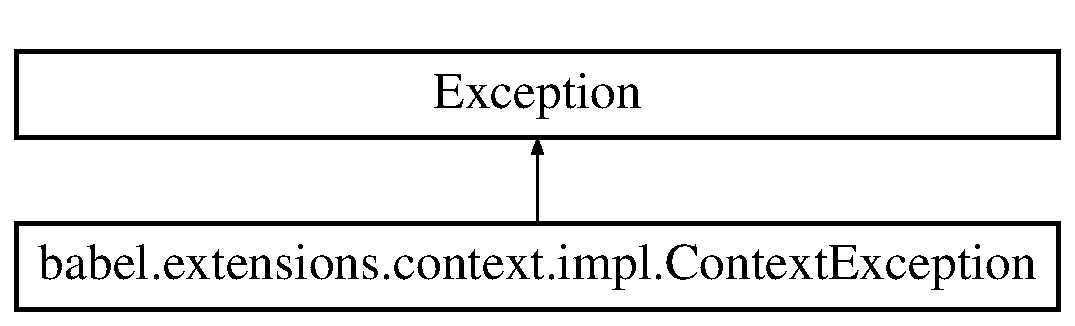
\includegraphics[height=2.000000cm]{classbabel_1_1extensions_1_1context_1_1impl_1_1_context_exception}
\end{center}
\end{figure}
\subsection*{Public Member Functions}
\begin{DoxyCompactItemize}
\item 
\hypertarget{classbabel_1_1extensions_1_1context_1_1impl_1_1_context_exception_af47ccb8ca840279eb088455ababeea19}{{\bfseries Context\-Exception} (string message, Context\-Exception\-Type exception\-Type)}\label{classbabel_1_1extensions_1_1context_1_1impl_1_1_context_exception_af47ccb8ca840279eb088455ababeea19}

\end{DoxyCompactItemize}
\subsection*{Properties}
\begin{DoxyCompactItemize}
\item 
\hypertarget{classbabel_1_1extensions_1_1context_1_1impl_1_1_context_exception_a6fd91528b2a1dc39d0c5a96999c95dce}{Context\-Exception\-Type {\bfseries type}\hspace{0.3cm}{\ttfamily  \mbox{[}get, set\mbox{]}}}\label{classbabel_1_1extensions_1_1context_1_1impl_1_1_context_exception_a6fd91528b2a1dc39d0c5a96999c95dce}

\end{DoxyCompactItemize}


The documentation for this class was generated from the following file\-:\begin{DoxyCompactItemize}
\item 
Assets/scripts/babel/extensions/context/impl/Context\-Exception.\-cs\end{DoxyCompactItemize}

\hypertarget{classbabel_1_1extensions_1_1context_1_1impl_1_1_context_view}{\section{babel.\-extensions.\-context.\-impl.\-Context\-View Class Reference}
\label{classbabel_1_1extensions_1_1context_1_1impl_1_1_context_view}\index{babel.\-extensions.\-context.\-impl.\-Context\-View@{babel.\-extensions.\-context.\-impl.\-Context\-View}}
}
Inheritance diagram for babel.\-extensions.\-context.\-impl.\-Context\-View\-:\begin{figure}[H]
\begin{center}
\leavevmode
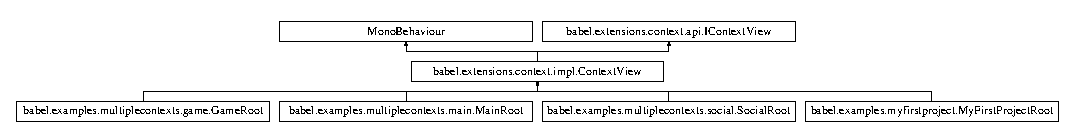
\includegraphics[height=1.400000cm]{classbabel_1_1extensions_1_1context_1_1impl_1_1_context_view}
\end{center}
\end{figure}
\subsection*{Properties}
\begin{DoxyCompactItemize}
\item 
\hypertarget{classbabel_1_1extensions_1_1context_1_1impl_1_1_context_view_a37b6b0fe69abb70efdfa957bffeb8045}{\hyperlink{interfacebabel_1_1extensions_1_1context_1_1api_1_1_i_context}{I\-Context} {\bfseries context}\hspace{0.3cm}{\ttfamily  \mbox{[}get, set\mbox{]}}}\label{classbabel_1_1extensions_1_1context_1_1impl_1_1_context_view_a37b6b0fe69abb70efdfa957bffeb8045}

\end{DoxyCompactItemize}


The documentation for this class was generated from the following file\-:\begin{DoxyCompactItemize}
\item 
Assets/scripts/babel/extensions/context/impl/Context\-View.\-cs\end{DoxyCompactItemize}

\hypertarget{classbabel_1_1examples_1_1multiplecontexts_1_1social_1_1_create_friend_list_command}{\section{babel.\-examples.\-multiplecontexts.\-social.\-Create\-Friend\-List\-Command Class Reference}
\label{classbabel_1_1examples_1_1multiplecontexts_1_1social_1_1_create_friend_list_command}\index{babel.\-examples.\-multiplecontexts.\-social.\-Create\-Friend\-List\-Command@{babel.\-examples.\-multiplecontexts.\-social.\-Create\-Friend\-List\-Command}}
}
Inheritance diagram for babel.\-examples.\-multiplecontexts.\-social.\-Create\-Friend\-List\-Command\-:\begin{figure}[H]
\begin{center}
\leavevmode
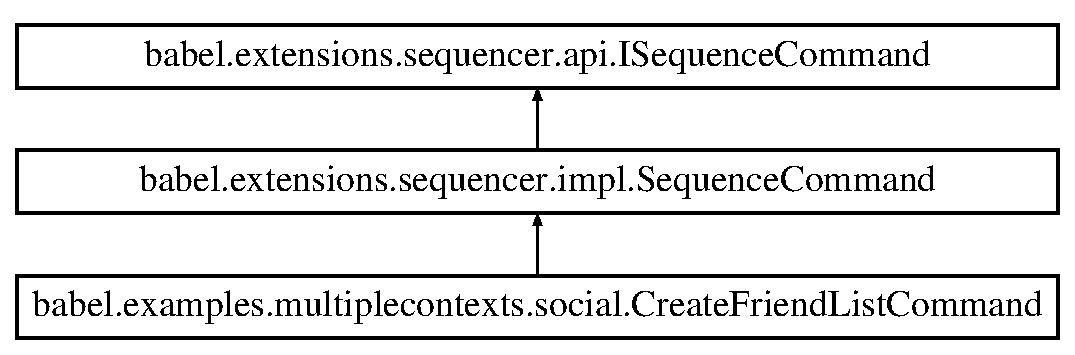
\includegraphics[height=3.000000cm]{classbabel_1_1examples_1_1multiplecontexts_1_1social_1_1_create_friend_list_command}
\end{center}
\end{figure}
\subsection*{Public Member Functions}
\begin{DoxyCompactItemize}
\item 
\hypertarget{classbabel_1_1examples_1_1multiplecontexts_1_1social_1_1_create_friend_list_command_a6289c2336b94bf03353f49e62276fe7e}{override void {\bfseries Execute} ()}\label{classbabel_1_1examples_1_1multiplecontexts_1_1social_1_1_create_friend_list_command_a6289c2336b94bf03353f49e62276fe7e}

\end{DoxyCompactItemize}
\subsection*{Properties}
\begin{DoxyCompactItemize}
\item 
\hypertarget{classbabel_1_1examples_1_1multiplecontexts_1_1social_1_1_create_friend_list_command_af99f28abd09e148486f76323daf00289}{Game\-Object {\bfseries context\-View}\hspace{0.3cm}{\ttfamily  \mbox{[}get, set\mbox{]}}}\label{classbabel_1_1examples_1_1multiplecontexts_1_1social_1_1_create_friend_list_command_af99f28abd09e148486f76323daf00289}

\item 
\hypertarget{classbabel_1_1examples_1_1multiplecontexts_1_1social_1_1_create_friend_list_command_a16263a55668eaff6994aca11c33bc69d}{\hyperlink{interfacebabel_1_1extensions_1_1dispatcher_1_1eventdispatcher_1_1api_1_1_i_event_dispatcher}{I\-Event\-Dispatcher} {\bfseries dispatcher}\hspace{0.3cm}{\ttfamily  \mbox{[}get, set\mbox{]}}}\label{classbabel_1_1examples_1_1multiplecontexts_1_1social_1_1_create_friend_list_command_a16263a55668eaff6994aca11c33bc69d}

\item 
\hypertarget{classbabel_1_1examples_1_1multiplecontexts_1_1social_1_1_create_friend_list_command_ab720a2c2718c12059a6ca8c6a3a4dfcb}{\hyperlink{classbabel_1_1examples_1_1multiplecontexts_1_1social_1_1_user_v_o}{User\-V\-O} {\bfseries user\-V\-O}\hspace{0.3cm}{\ttfamily  \mbox{[}get, set\mbox{]}}}\label{classbabel_1_1examples_1_1multiplecontexts_1_1social_1_1_create_friend_list_command_ab720a2c2718c12059a6ca8c6a3a4dfcb}

\end{DoxyCompactItemize}


The documentation for this class was generated from the following file\-:\begin{DoxyCompactItemize}
\item 
Assets/scripts/babel/examples/multiplecontexts/social/controller/Create\-Friend\-List\-Command.\-cs\end{DoxyCompactItemize}

\hypertarget{classbabel_1_1examples_1_1multiplecontexts_1_1social_1_1_create_user_tile_command}{\section{babel.\-examples.\-multiplecontexts.\-social.\-Create\-User\-Tile\-Command Class Reference}
\label{classbabel_1_1examples_1_1multiplecontexts_1_1social_1_1_create_user_tile_command}\index{babel.\-examples.\-multiplecontexts.\-social.\-Create\-User\-Tile\-Command@{babel.\-examples.\-multiplecontexts.\-social.\-Create\-User\-Tile\-Command}}
}
Inheritance diagram for babel.\-examples.\-multiplecontexts.\-social.\-Create\-User\-Tile\-Command\-:\begin{figure}[H]
\begin{center}
\leavevmode
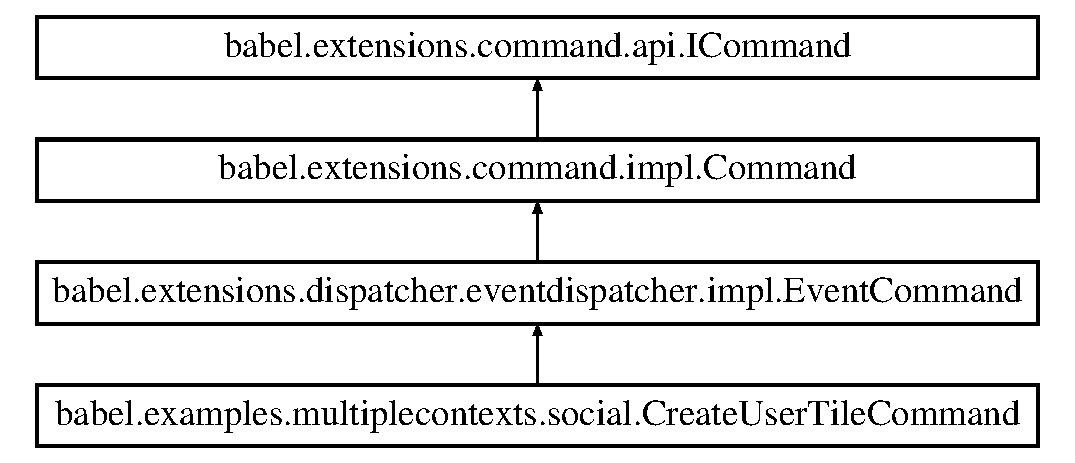
\includegraphics[height=4.000000cm]{classbabel_1_1examples_1_1multiplecontexts_1_1social_1_1_create_user_tile_command}
\end{center}
\end{figure}
\subsection*{Public Member Functions}
\begin{DoxyCompactItemize}
\item 
\hypertarget{classbabel_1_1examples_1_1multiplecontexts_1_1social_1_1_create_user_tile_command_ac8dbd547f7fb1ab88ee447979be573a5}{override void {\bfseries Execute} ()}\label{classbabel_1_1examples_1_1multiplecontexts_1_1social_1_1_create_user_tile_command_ac8dbd547f7fb1ab88ee447979be573a5}

\end{DoxyCompactItemize}
\subsection*{Properties}
\begin{DoxyCompactItemize}
\item 
\hypertarget{classbabel_1_1examples_1_1multiplecontexts_1_1social_1_1_create_user_tile_command_a7f9519ba7f110bd8ad867f75d4f5f8a4}{Game\-Object {\bfseries context\-View}\hspace{0.3cm}{\ttfamily  \mbox{[}get, set\mbox{]}}}\label{classbabel_1_1examples_1_1multiplecontexts_1_1social_1_1_create_user_tile_command_a7f9519ba7f110bd8ad867f75d4f5f8a4}

\end{DoxyCompactItemize}


The documentation for this class was generated from the following file\-:\begin{DoxyCompactItemize}
\item 
Assets/scripts/babel/examples/multiplecontexts/social/controller/Create\-User\-Tile\-Command.\-cs\end{DoxyCompactItemize}

\hypertarget{class_de_construct}{\section{De\-Construct Class Reference}
\label{class_de_construct}\index{De\-Construct@{De\-Construct}}
}
Inheritance diagram for De\-Construct\-:\begin{figure}[H]
\begin{center}
\leavevmode
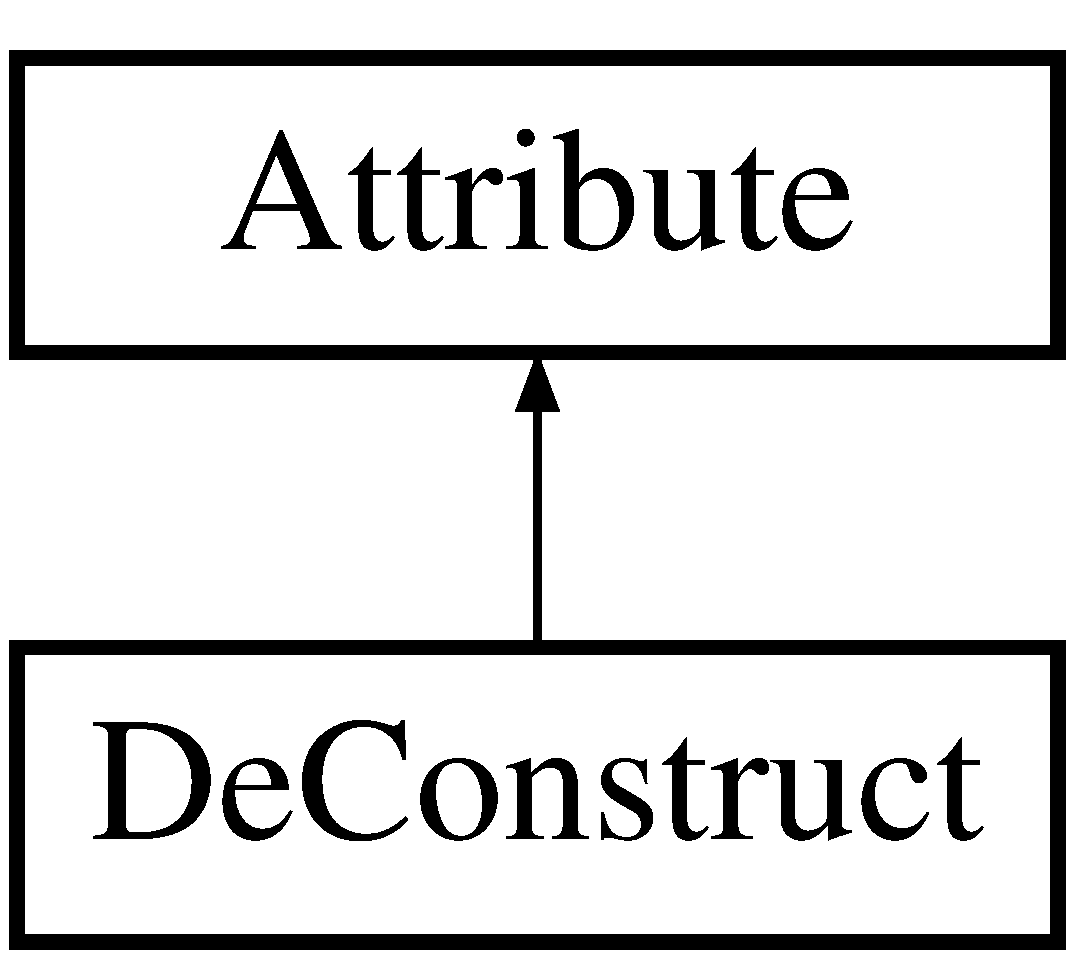
\includegraphics[height=2.000000cm]{class_de_construct}
\end{center}
\end{figure}


The documentation for this class was generated from the following file\-:\begin{DoxyCompactItemize}
\item 
Assets/scripts/strange/extensions/injector/Inject\-Attribute.\-cs\end{DoxyCompactItemize}

\hypertarget{classbabel_1_1extensions_1_1dispatcher_1_1impl_1_1_dispatcher_exception}{\section{babel.\-extensions.\-dispatcher.\-impl.\-Dispatcher\-Exception Class Reference}
\label{classbabel_1_1extensions_1_1dispatcher_1_1impl_1_1_dispatcher_exception}\index{babel.\-extensions.\-dispatcher.\-impl.\-Dispatcher\-Exception@{babel.\-extensions.\-dispatcher.\-impl.\-Dispatcher\-Exception}}
}
Inheritance diagram for babel.\-extensions.\-dispatcher.\-impl.\-Dispatcher\-Exception\-:\begin{figure}[H]
\begin{center}
\leavevmode
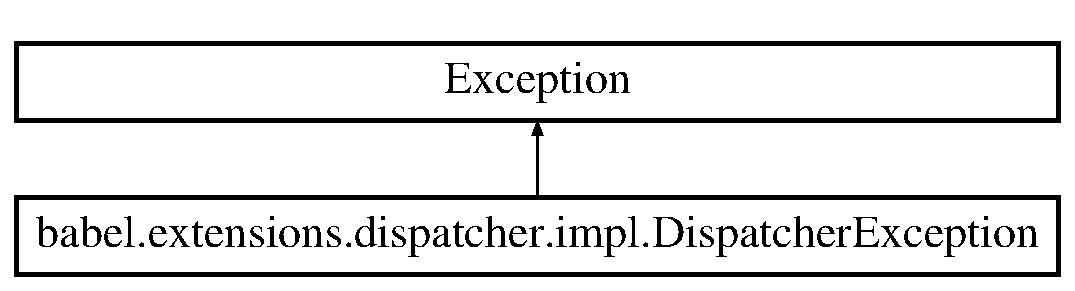
\includegraphics[height=2.000000cm]{classbabel_1_1extensions_1_1dispatcher_1_1impl_1_1_dispatcher_exception}
\end{center}
\end{figure}
\subsection*{Public Member Functions}
\begin{DoxyCompactItemize}
\item 
\hypertarget{classbabel_1_1extensions_1_1dispatcher_1_1impl_1_1_dispatcher_exception_a93ace204c997e81bec48f4b0f8f6692c}{{\bfseries Dispatcher\-Exception} (string message, Dispatcher\-Exception\-Type exception\-Type)}\label{classbabel_1_1extensions_1_1dispatcher_1_1impl_1_1_dispatcher_exception_a93ace204c997e81bec48f4b0f8f6692c}

\end{DoxyCompactItemize}
\subsection*{Properties}
\begin{DoxyCompactItemize}
\item 
\hypertarget{classbabel_1_1extensions_1_1dispatcher_1_1impl_1_1_dispatcher_exception_a441a04dc3df4fe74f3f88ec376cbc264}{Dispatcher\-Exception\-Type {\bfseries type}\hspace{0.3cm}{\ttfamily  \mbox{[}get, set\mbox{]}}}\label{classbabel_1_1extensions_1_1dispatcher_1_1impl_1_1_dispatcher_exception_a441a04dc3df4fe74f3f88ec376cbc264}

\end{DoxyCompactItemize}


The documentation for this class was generated from the following file\-:\begin{DoxyCompactItemize}
\item 
Assets/scripts/babel/extensions/dispatcher/impl/Dispatcher\-Exception.\-cs\end{DoxyCompactItemize}

\hypertarget{classbabel_1_1examples_1_1multiplecontexts_1_1game_1_1_enemy_mediator}{\section{babel.\-examples.\-multiplecontexts.\-game.\-Enemy\-Mediator Class Reference}
\label{classbabel_1_1examples_1_1multiplecontexts_1_1game_1_1_enemy_mediator}\index{babel.\-examples.\-multiplecontexts.\-game.\-Enemy\-Mediator@{babel.\-examples.\-multiplecontexts.\-game.\-Enemy\-Mediator}}
}
Inheritance diagram for babel.\-examples.\-multiplecontexts.\-game.\-Enemy\-Mediator\-:\begin{figure}[H]
\begin{center}
\leavevmode
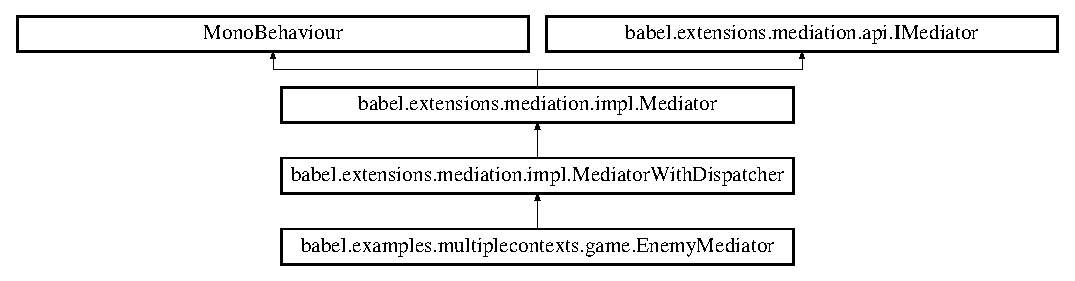
\includegraphics[height=3.333333cm]{classbabel_1_1examples_1_1multiplecontexts_1_1game_1_1_enemy_mediator}
\end{center}
\end{figure}
\subsection*{Public Member Functions}
\begin{DoxyCompactItemize}
\item 
override void \hyperlink{classbabel_1_1examples_1_1multiplecontexts_1_1game_1_1_enemy_mediator_a5acadeb51fd09fd30f6da9c5d7ca9f3a}{on\-Register} ()
\begin{DoxyCompactList}\small\item\em Fires after all injections satisifed. \end{DoxyCompactList}\item 
override void \hyperlink{classbabel_1_1examples_1_1multiplecontexts_1_1game_1_1_enemy_mediator_a2c5abab1d577a583238d326312f78915}{on\-Remove} ()
\begin{DoxyCompactList}\small\item\em Fires on removal of view. \end{DoxyCompactList}\end{DoxyCompactItemize}
\subsection*{Additional Inherited Members}


\subsection{Member Function Documentation}
\hypertarget{classbabel_1_1examples_1_1multiplecontexts_1_1game_1_1_enemy_mediator_a5acadeb51fd09fd30f6da9c5d7ca9f3a}{\index{babel\-::examples\-::multiplecontexts\-::game\-::\-Enemy\-Mediator@{babel\-::examples\-::multiplecontexts\-::game\-::\-Enemy\-Mediator}!on\-Register@{on\-Register}}
\index{on\-Register@{on\-Register}!babel::examples::multiplecontexts::game::EnemyMediator@{babel\-::examples\-::multiplecontexts\-::game\-::\-Enemy\-Mediator}}
\subsubsection[{on\-Register}]{\setlength{\rightskip}{0pt plus 5cm}override void babel.\-examples.\-multiplecontexts.\-game.\-Enemy\-Mediator.\-on\-Register (
\begin{DoxyParamCaption}
{}
\end{DoxyParamCaption}
)\hspace{0.3cm}{\ttfamily [inline]}, {\ttfamily [virtual]}}}\label{classbabel_1_1examples_1_1multiplecontexts_1_1game_1_1_enemy_mediator_a5acadeb51fd09fd30f6da9c5d7ca9f3a}


Fires after all injections satisifed. 

Override and place your initialization code here. 

Reimplemented from \hyperlink{classbabel_1_1extensions_1_1mediation_1_1impl_1_1_mediator_a693800cf98ef09c660de249436108d9a}{babel.\-extensions.\-mediation.\-impl.\-Mediator}.

\hypertarget{classbabel_1_1examples_1_1multiplecontexts_1_1game_1_1_enemy_mediator_a2c5abab1d577a583238d326312f78915}{\index{babel\-::examples\-::multiplecontexts\-::game\-::\-Enemy\-Mediator@{babel\-::examples\-::multiplecontexts\-::game\-::\-Enemy\-Mediator}!on\-Remove@{on\-Remove}}
\index{on\-Remove@{on\-Remove}!babel::examples::multiplecontexts::game::EnemyMediator@{babel\-::examples\-::multiplecontexts\-::game\-::\-Enemy\-Mediator}}
\subsubsection[{on\-Remove}]{\setlength{\rightskip}{0pt plus 5cm}override void babel.\-examples.\-multiplecontexts.\-game.\-Enemy\-Mediator.\-on\-Remove (
\begin{DoxyParamCaption}
{}
\end{DoxyParamCaption}
)\hspace{0.3cm}{\ttfamily [inline]}, {\ttfamily [virtual]}}}\label{classbabel_1_1examples_1_1multiplecontexts_1_1game_1_1_enemy_mediator_a2c5abab1d577a583238d326312f78915}


Fires on removal of view. 

Override and place your cleanup code here 

Reimplemented from \hyperlink{classbabel_1_1extensions_1_1mediation_1_1impl_1_1_mediator_a8b818665eda883eac66c83b8468007e9}{babel.\-extensions.\-mediation.\-impl.\-Mediator}.



The documentation for this class was generated from the following file\-:\begin{DoxyCompactItemize}
\item 
Assets/scripts/babel/examples/multiplecontexts/game/view/Enemy\-Mediator.\-cs\end{DoxyCompactItemize}

\hypertarget{classbabel_1_1examples_1_1multiplecontexts_1_1game_1_1_enemy_view}{\section{babel.\-examples.\-multiplecontexts.\-game.\-Enemy\-View Class Reference}
\label{classbabel_1_1examples_1_1multiplecontexts_1_1game_1_1_enemy_view}\index{babel.\-examples.\-multiplecontexts.\-game.\-Enemy\-View@{babel.\-examples.\-multiplecontexts.\-game.\-Enemy\-View}}
}
Inheritance diagram for babel.\-examples.\-multiplecontexts.\-game.\-Enemy\-View\-:\begin{figure}[H]
\begin{center}
\leavevmode
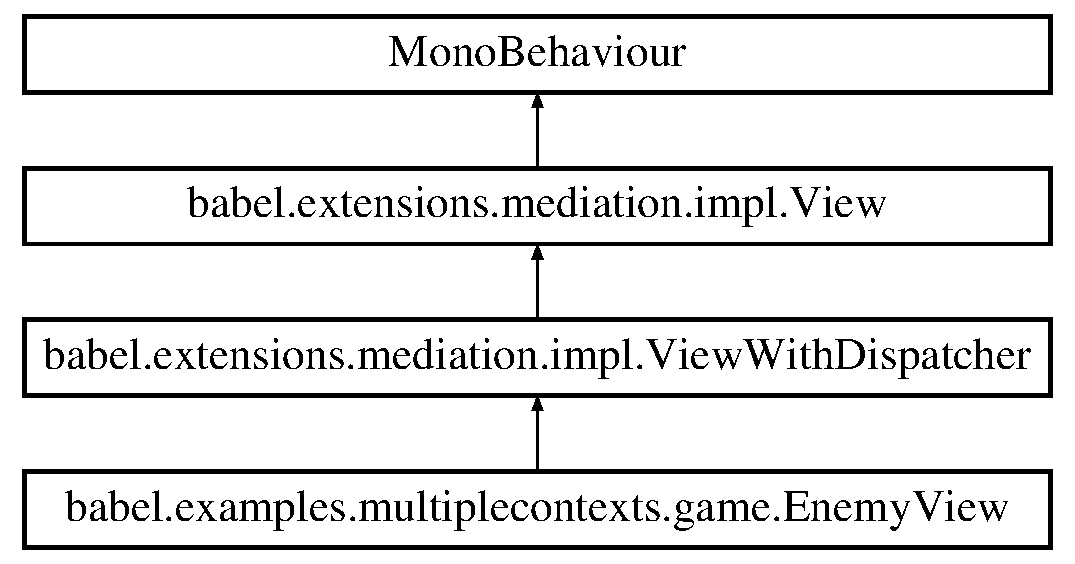
\includegraphics[height=4.000000cm]{classbabel_1_1examples_1_1multiplecontexts_1_1game_1_1_enemy_view}
\end{center}
\end{figure}
\subsection*{Public Attributes}
\begin{DoxyCompactItemize}
\item 
\hypertarget{classbabel_1_1examples_1_1multiplecontexts_1_1game_1_1_enemy_view_aba952bff051a306f8eb302b3747f5021}{float {\bfseries edx\-\_\-\-Wobble\-Force} = .\-4f}\label{classbabel_1_1examples_1_1multiplecontexts_1_1game_1_1_enemy_view_aba952bff051a306f8eb302b3747f5021}

\item 
\hypertarget{classbabel_1_1examples_1_1multiplecontexts_1_1game_1_1_enemy_view_a0d07f4194f062da28c021eaee7aeeac6}{float {\bfseries edx\-\_\-\-Wobble\-Increment} = .\-1f}\label{classbabel_1_1examples_1_1multiplecontexts_1_1game_1_1_enemy_view_a0d07f4194f062da28c021eaee7aeeac6}

\end{DoxyCompactItemize}
\subsection*{Additional Inherited Members}


The documentation for this class was generated from the following file\-:\begin{DoxyCompactItemize}
\item 
Assets/scripts/babel/examples/multiplecontexts/game/view/Enemy\-View.\-cs\end{DoxyCompactItemize}

\hypertarget{classbabel_1_1extensions_1_1dispatcher_1_1eventdispatcher_1_1impl_1_1_event_binding}{\section{babel.\-extensions.\-dispatcher.\-eventdispatcher.\-impl.\-Event\-Binding Class Reference}
\label{classbabel_1_1extensions_1_1dispatcher_1_1eventdispatcher_1_1impl_1_1_event_binding}\index{babel.\-extensions.\-dispatcher.\-eventdispatcher.\-impl.\-Event\-Binding@{babel.\-extensions.\-dispatcher.\-eventdispatcher.\-impl.\-Event\-Binding}}
}
Inheritance diagram for babel.\-extensions.\-dispatcher.\-eventdispatcher.\-impl.\-Event\-Binding\-:\begin{figure}[H]
\begin{center}
\leavevmode
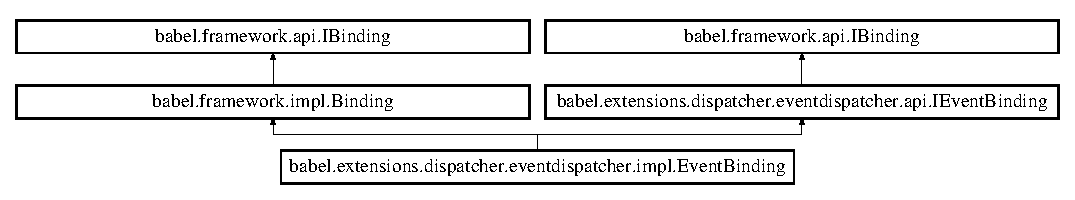
\includegraphics[height=2.240000cm]{classbabel_1_1extensions_1_1dispatcher_1_1eventdispatcher_1_1impl_1_1_event_binding}
\end{center}
\end{figure}
\subsection*{Public Member Functions}
\begin{DoxyCompactItemize}
\item 
\hypertarget{classbabel_1_1extensions_1_1dispatcher_1_1eventdispatcher_1_1impl_1_1_event_binding_aa2e3506107a571b26fee0d43641165f6}{{\bfseries Event\-Binding} (babel.\-framework.\-impl.\-Binder.\-Binding\-Resolver resolver)}\label{classbabel_1_1extensions_1_1dispatcher_1_1eventdispatcher_1_1impl_1_1_event_binding_aa2e3506107a571b26fee0d43641165f6}

\item 
\hypertarget{classbabel_1_1extensions_1_1dispatcher_1_1eventdispatcher_1_1impl_1_1_event_binding_a6c088d42cf54b7bed35b9789c6bb655e}{Event\-Callback\-Type {\bfseries type\-For\-Callback} (Empty\-Callback callback)}\label{classbabel_1_1extensions_1_1dispatcher_1_1eventdispatcher_1_1impl_1_1_event_binding_a6c088d42cf54b7bed35b9789c6bb655e}

\item 
\hypertarget{classbabel_1_1extensions_1_1dispatcher_1_1eventdispatcher_1_1impl_1_1_event_binding_a3fc5a74be2dee623c8fb0cae12e04e3d}{Event\-Callback\-Type {\bfseries type\-For\-Callback} (Event\-Callback callback)}\label{classbabel_1_1extensions_1_1dispatcher_1_1eventdispatcher_1_1impl_1_1_event_binding_a3fc5a74be2dee623c8fb0cae12e04e3d}

\item 
\hypertarget{classbabel_1_1extensions_1_1dispatcher_1_1eventdispatcher_1_1impl_1_1_event_binding_a6b68775b2169bfa529a276f8d9fc3d37}{new \hyperlink{interfacebabel_1_1extensions_1_1dispatcher_1_1eventdispatcher_1_1api_1_1_i_event_binding}{I\-Event\-Binding} {\bfseries Key} (object key)}\label{classbabel_1_1extensions_1_1dispatcher_1_1eventdispatcher_1_1impl_1_1_event_binding_a6b68775b2169bfa529a276f8d9fc3d37}

\item 
\hypertarget{classbabel_1_1extensions_1_1dispatcher_1_1eventdispatcher_1_1impl_1_1_event_binding_a1f2bc0fc265c5446ac8bed2695cffb5d}{\hyperlink{interfacebabel_1_1extensions_1_1dispatcher_1_1eventdispatcher_1_1api_1_1_i_event_binding}{I\-Event\-Binding} {\bfseries To} (Event\-Callback value)}\label{classbabel_1_1extensions_1_1dispatcher_1_1eventdispatcher_1_1impl_1_1_event_binding_a1f2bc0fc265c5446ac8bed2695cffb5d}

\item 
\hypertarget{classbabel_1_1extensions_1_1dispatcher_1_1eventdispatcher_1_1impl_1_1_event_binding_a56fbeca0078bee5f47966b6c4a3c5df7}{\hyperlink{interfacebabel_1_1extensions_1_1dispatcher_1_1eventdispatcher_1_1api_1_1_i_event_binding}{I\-Event\-Binding} {\bfseries To} (Empty\-Callback value)}\label{classbabel_1_1extensions_1_1dispatcher_1_1eventdispatcher_1_1impl_1_1_event_binding_a56fbeca0078bee5f47966b6c4a3c5df7}

\item 
\hypertarget{classbabel_1_1extensions_1_1dispatcher_1_1eventdispatcher_1_1impl_1_1_event_binding_a9e333d44a36c47923acbc9819e6d636c}{new \hyperlink{interfacebabel_1_1extensions_1_1dispatcher_1_1eventdispatcher_1_1api_1_1_i_event_binding}{I\-Event\-Binding} {\bfseries To} (object value)}\label{classbabel_1_1extensions_1_1dispatcher_1_1eventdispatcher_1_1impl_1_1_event_binding_a9e333d44a36c47923acbc9819e6d636c}

\item 
\hypertarget{classbabel_1_1extensions_1_1dispatcher_1_1eventdispatcher_1_1impl_1_1_event_binding_a13dcc230f18778bb01e740691733fa34}{override void {\bfseries Remove\-Value} (object value)}\label{classbabel_1_1extensions_1_1dispatcher_1_1eventdispatcher_1_1impl_1_1_event_binding_a13dcc230f18778bb01e740691733fa34}

\end{DoxyCompactItemize}
\subsection*{Additional Inherited Members}


The documentation for this class was generated from the following file\-:\begin{DoxyCompactItemize}
\item 
Assets/scripts/babel/extensions/dispatcher/eventdispatcher/impl/Event\-Binding.\-cs\end{DoxyCompactItemize}

\hypertarget{classbabel_1_1extensions_1_1dispatcher_1_1eventdispatcher_1_1impl_1_1_event_command}{\section{babel.\-extensions.\-dispatcher.\-eventdispatcher.\-impl.\-Event\-Command Class Reference}
\label{classbabel_1_1extensions_1_1dispatcher_1_1eventdispatcher_1_1impl_1_1_event_command}\index{babel.\-extensions.\-dispatcher.\-eventdispatcher.\-impl.\-Event\-Command@{babel.\-extensions.\-dispatcher.\-eventdispatcher.\-impl.\-Event\-Command}}
}
Inheritance diagram for babel.\-extensions.\-dispatcher.\-eventdispatcher.\-impl.\-Event\-Command\-:\begin{figure}[H]
\begin{center}
\leavevmode
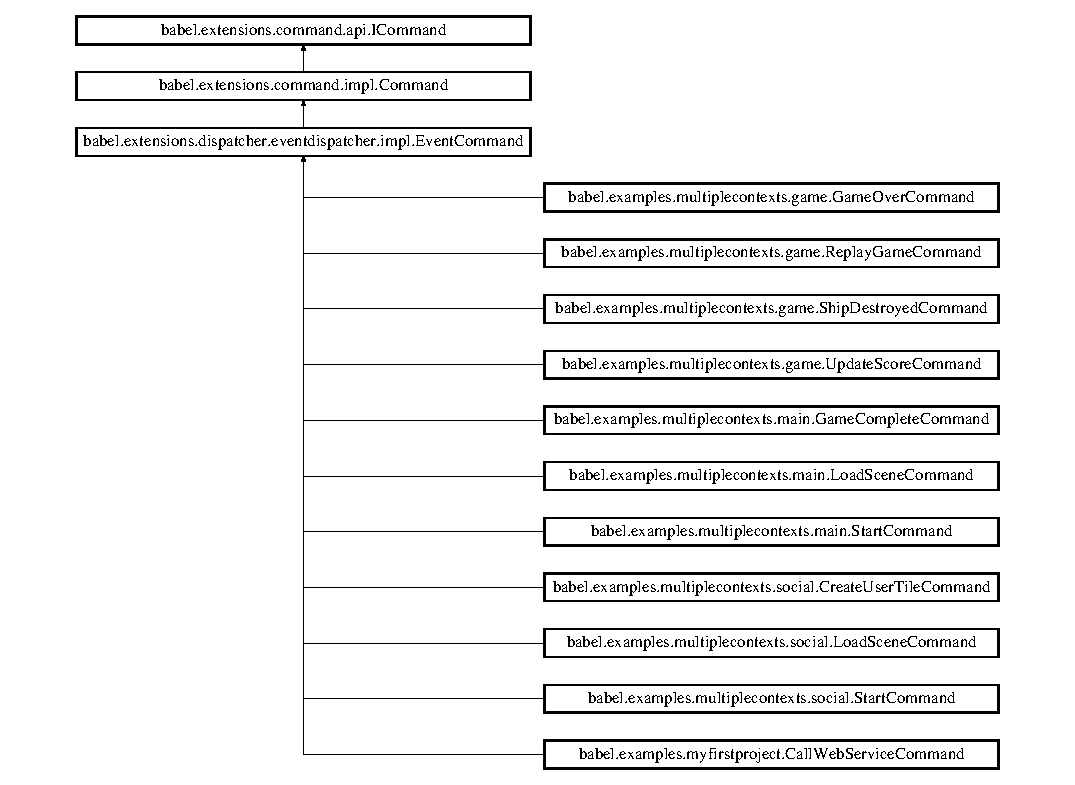
\includegraphics[height=10.103093cm]{classbabel_1_1extensions_1_1dispatcher_1_1eventdispatcher_1_1impl_1_1_event_command}
\end{center}
\end{figure}
\subsection*{Properties}
\begin{DoxyCompactItemize}
\item 
\hypertarget{classbabel_1_1extensions_1_1dispatcher_1_1eventdispatcher_1_1impl_1_1_event_command_a8e4b6a0b5469b654bb96bdf0c095916f}{\hyperlink{interfacebabel_1_1extensions_1_1dispatcher_1_1eventdispatcher_1_1api_1_1_i_event_dispatcher}{I\-Event\-Dispatcher} {\bfseries dispatcher}\hspace{0.3cm}{\ttfamily  \mbox{[}get, set\mbox{]}}}\label{classbabel_1_1extensions_1_1dispatcher_1_1eventdispatcher_1_1impl_1_1_event_command_a8e4b6a0b5469b654bb96bdf0c095916f}

\item 
\hypertarget{classbabel_1_1extensions_1_1dispatcher_1_1eventdispatcher_1_1impl_1_1_event_command_a1459c725fc37fdcda43c9547d93419a0}{\hyperlink{classbabel_1_1extensions_1_1dispatcher_1_1eventdispatcher_1_1impl_1_1_tm_event}{Tm\-Event} {\bfseries evt}\hspace{0.3cm}{\ttfamily  \mbox{[}get, set\mbox{]}}}\label{classbabel_1_1extensions_1_1dispatcher_1_1eventdispatcher_1_1impl_1_1_event_command_a1459c725fc37fdcda43c9547d93419a0}

\end{DoxyCompactItemize}
\subsection*{Additional Inherited Members}


The documentation for this class was generated from the following file\-:\begin{DoxyCompactItemize}
\item 
Assets/scripts/babel/extensions/dispatcher/eventdispatcher/impl/Event\-Command.\-cs\end{DoxyCompactItemize}

\hypertarget{classbabel_1_1extensions_1_1dispatcher_1_1eventdispatcher_1_1impl_1_1_event_dispatcher}{\section{babel.\-extensions.\-dispatcher.\-eventdispatcher.\-impl.\-Event\-Dispatcher Class Reference}
\label{classbabel_1_1extensions_1_1dispatcher_1_1eventdispatcher_1_1impl_1_1_event_dispatcher}\index{babel.\-extensions.\-dispatcher.\-eventdispatcher.\-impl.\-Event\-Dispatcher@{babel.\-extensions.\-dispatcher.\-eventdispatcher.\-impl.\-Event\-Dispatcher}}
}
Inheritance diagram for babel.\-extensions.\-dispatcher.\-eventdispatcher.\-impl.\-Event\-Dispatcher\-:\begin{figure}[H]
\begin{center}
\leavevmode
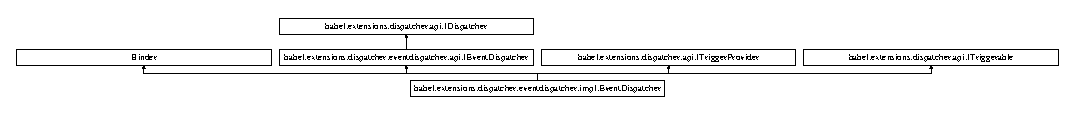
\includegraphics[height=1.065990cm]{classbabel_1_1extensions_1_1dispatcher_1_1eventdispatcher_1_1impl_1_1_event_dispatcher}
\end{center}
\end{figure}
\subsection*{Public Member Functions}
\begin{DoxyCompactItemize}
\item 
\hypertarget{classbabel_1_1extensions_1_1dispatcher_1_1eventdispatcher_1_1impl_1_1_event_dispatcher_a6f97076ac7e5b1955b2e2d8605f459d8}{override \hyperlink{interfacebabel_1_1framework_1_1api_1_1_i_binding}{I\-Binding} {\bfseries Get\-Raw\-Binding} ()}\label{classbabel_1_1extensions_1_1dispatcher_1_1eventdispatcher_1_1impl_1_1_event_dispatcher_a6f97076ac7e5b1955b2e2d8605f459d8}

\item 
\hypertarget{classbabel_1_1extensions_1_1dispatcher_1_1eventdispatcher_1_1impl_1_1_event_dispatcher_ac44d96912bb6cc3a48bd6f043cb5b348}{new \hyperlink{interfacebabel_1_1extensions_1_1dispatcher_1_1eventdispatcher_1_1api_1_1_i_event_binding}{I\-Event\-Binding} {\bfseries Bind} (object key)}\label{classbabel_1_1extensions_1_1dispatcher_1_1eventdispatcher_1_1impl_1_1_event_dispatcher_ac44d96912bb6cc3a48bd6f043cb5b348}

\item 
\hypertarget{classbabel_1_1extensions_1_1dispatcher_1_1eventdispatcher_1_1impl_1_1_event_dispatcher_afb225c067e69786884c05f8c635fad71}{void {\bfseries Dispatch} (object event\-Type)}\label{classbabel_1_1extensions_1_1dispatcher_1_1eventdispatcher_1_1impl_1_1_event_dispatcher_afb225c067e69786884c05f8c635fad71}

\item 
\hypertarget{classbabel_1_1extensions_1_1dispatcher_1_1eventdispatcher_1_1impl_1_1_event_dispatcher_aeae986ad4b65d5c2c33514da21841905}{void {\bfseries Dispatch} (object event\-Type, object data)}\label{classbabel_1_1extensions_1_1dispatcher_1_1eventdispatcher_1_1impl_1_1_event_dispatcher_aeae986ad4b65d5c2c33514da21841905}

\item 
\hypertarget{classbabel_1_1extensions_1_1dispatcher_1_1eventdispatcher_1_1impl_1_1_event_dispatcher_aea227da4cbd48129e4c1472d71e01926}{void {\bfseries add\-Listener} (object evt, Event\-Callback callback)}\label{classbabel_1_1extensions_1_1dispatcher_1_1eventdispatcher_1_1impl_1_1_event_dispatcher_aea227da4cbd48129e4c1472d71e01926}

\item 
\hypertarget{classbabel_1_1extensions_1_1dispatcher_1_1eventdispatcher_1_1impl_1_1_event_dispatcher_a664159a404acae8eb4f77637fd4fe578}{void {\bfseries add\-Listener} (object evt, Empty\-Callback callback)}\label{classbabel_1_1extensions_1_1dispatcher_1_1eventdispatcher_1_1impl_1_1_event_dispatcher_a664159a404acae8eb4f77637fd4fe578}

\item 
\hypertarget{classbabel_1_1extensions_1_1dispatcher_1_1eventdispatcher_1_1impl_1_1_event_dispatcher_a70487f5939bcbb2532826207cf7eb248}{void {\bfseries remove\-Listener} (object evt, Event\-Callback callback)}\label{classbabel_1_1extensions_1_1dispatcher_1_1eventdispatcher_1_1impl_1_1_event_dispatcher_a70487f5939bcbb2532826207cf7eb248}

\item 
\hypertarget{classbabel_1_1extensions_1_1dispatcher_1_1eventdispatcher_1_1impl_1_1_event_dispatcher_aaa25504a38e434eb5e646881387b88c5}{void {\bfseries remove\-Listener} (object evt, Empty\-Callback callback)}\label{classbabel_1_1extensions_1_1dispatcher_1_1eventdispatcher_1_1impl_1_1_event_dispatcher_aaa25504a38e434eb5e646881387b88c5}

\item 
\hypertarget{classbabel_1_1extensions_1_1dispatcher_1_1eventdispatcher_1_1impl_1_1_event_dispatcher_a4843886d728f1a594e5927a6f4e27df3}{bool {\bfseries has\-Listener} (object evt, Event\-Callback callback)}\label{classbabel_1_1extensions_1_1dispatcher_1_1eventdispatcher_1_1impl_1_1_event_dispatcher_a4843886d728f1a594e5927a6f4e27df3}

\item 
\hypertarget{classbabel_1_1extensions_1_1dispatcher_1_1eventdispatcher_1_1impl_1_1_event_dispatcher_a64af60bef10d7a56623ee911fd98c901}{bool {\bfseries has\-Listener} (object evt, Empty\-Callback callback)}\label{classbabel_1_1extensions_1_1dispatcher_1_1eventdispatcher_1_1impl_1_1_event_dispatcher_a64af60bef10d7a56623ee911fd98c901}

\item 
\hypertarget{classbabel_1_1extensions_1_1dispatcher_1_1eventdispatcher_1_1impl_1_1_event_dispatcher_a89bc0e1e1d25f8d33be29bc0230e8ae0}{void {\bfseries update\-Listener} (bool to\-Add, object evt, Event\-Callback callback)}\label{classbabel_1_1extensions_1_1dispatcher_1_1eventdispatcher_1_1impl_1_1_event_dispatcher_a89bc0e1e1d25f8d33be29bc0230e8ae0}

\item 
\hypertarget{classbabel_1_1extensions_1_1dispatcher_1_1eventdispatcher_1_1impl_1_1_event_dispatcher_a0a048e523ff1dd2a079fc234ff7f52cd}{void {\bfseries update\-Listener} (bool to\-Add, object evt, Empty\-Callback callback)}\label{classbabel_1_1extensions_1_1dispatcher_1_1eventdispatcher_1_1impl_1_1_event_dispatcher_a0a048e523ff1dd2a079fc234ff7f52cd}

\item 
\hypertarget{classbabel_1_1extensions_1_1dispatcher_1_1eventdispatcher_1_1impl_1_1_event_dispatcher_a4f6cf32dd09cd39865e9904d61040201}{void {\bfseries Add\-Triggerable} (\hyperlink{interfacebabel_1_1extensions_1_1dispatcher_1_1api_1_1_i_triggerable}{I\-Triggerable} target)}\label{classbabel_1_1extensions_1_1dispatcher_1_1eventdispatcher_1_1impl_1_1_event_dispatcher_a4f6cf32dd09cd39865e9904d61040201}

\item 
\hypertarget{classbabel_1_1extensions_1_1dispatcher_1_1eventdispatcher_1_1impl_1_1_event_dispatcher_a96343db6aeb761802ce4221e6727f1b8}{void {\bfseries Remove\-Triggerable} (\hyperlink{interfacebabel_1_1extensions_1_1dispatcher_1_1api_1_1_i_triggerable}{I\-Triggerable} target)}\label{classbabel_1_1extensions_1_1dispatcher_1_1eventdispatcher_1_1impl_1_1_event_dispatcher_a96343db6aeb761802ce4221e6727f1b8}

\item 
\hypertarget{classbabel_1_1extensions_1_1dispatcher_1_1eventdispatcher_1_1impl_1_1_event_dispatcher_a886756ec05bb5d486af51897912b1e02}{void {\bfseries Trigger$<$ T $>$} (object data)}\label{classbabel_1_1extensions_1_1dispatcher_1_1eventdispatcher_1_1impl_1_1_event_dispatcher_a886756ec05bb5d486af51897912b1e02}

\item 
\hypertarget{classbabel_1_1extensions_1_1dispatcher_1_1eventdispatcher_1_1impl_1_1_event_dispatcher_a89b1da67fed12ce75e0775cb0d45c5fb}{void {\bfseries Trigger} (object key, object data)}\label{classbabel_1_1extensions_1_1dispatcher_1_1eventdispatcher_1_1impl_1_1_event_dispatcher_a89b1da67fed12ce75e0775cb0d45c5fb}

\end{DoxyCompactItemize}
\subsection*{Protected Attributes}
\begin{DoxyCompactItemize}
\item 
\hypertarget{classbabel_1_1extensions_1_1dispatcher_1_1eventdispatcher_1_1impl_1_1_event_dispatcher_a224d81717fb9b5b283057cf7915cac30}{\hyperlink{interfacebabel_1_1extensions_1_1dispatcher_1_1api_1_1_i_triggerable}{I\-Triggerable}\mbox{[}$\,$\mbox{]} {\bfseries trigger\-Clients}}\label{classbabel_1_1extensions_1_1dispatcher_1_1eventdispatcher_1_1impl_1_1_event_dispatcher_a224d81717fb9b5b283057cf7915cac30}

\end{DoxyCompactItemize}


The documentation for this class was generated from the following file\-:\begin{DoxyCompactItemize}
\item 
Assets/scripts/babel/extensions/dispatcher/eventdispatcher/impl/Event\-Dispatcher.\-cs\end{DoxyCompactItemize}

\hypertarget{classbabel_1_1extensions_1_1dispatcher_1_1eventdispatcher_1_1impl_1_1_event_dispatcher_exception}{\section{babel.\-extensions.\-dispatcher.\-eventdispatcher.\-impl.\-Event\-Dispatcher\-Exception Class Reference}
\label{classbabel_1_1extensions_1_1dispatcher_1_1eventdispatcher_1_1impl_1_1_event_dispatcher_exception}\index{babel.\-extensions.\-dispatcher.\-eventdispatcher.\-impl.\-Event\-Dispatcher\-Exception@{babel.\-extensions.\-dispatcher.\-eventdispatcher.\-impl.\-Event\-Dispatcher\-Exception}}
}
Inheritance diagram for babel.\-extensions.\-dispatcher.\-eventdispatcher.\-impl.\-Event\-Dispatcher\-Exception\-:\begin{figure}[H]
\begin{center}
\leavevmode
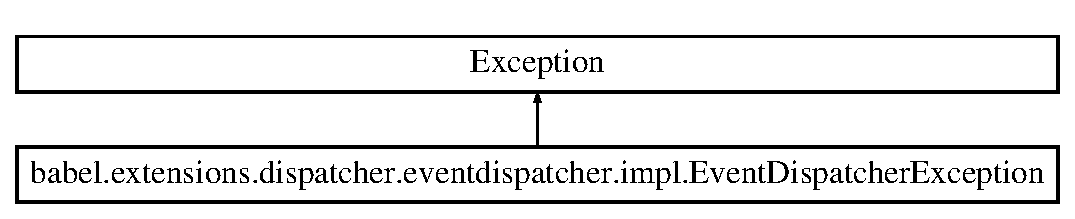
\includegraphics[height=2.000000cm]{classbabel_1_1extensions_1_1dispatcher_1_1eventdispatcher_1_1impl_1_1_event_dispatcher_exception}
\end{center}
\end{figure}
\subsection*{Public Member Functions}
\begin{DoxyCompactItemize}
\item 
\hypertarget{classbabel_1_1extensions_1_1dispatcher_1_1eventdispatcher_1_1impl_1_1_event_dispatcher_exception_ac0e7f116082deb24a4c4c85bf9bad54a}{{\bfseries Event\-Dispatcher\-Exception} (string message, Event\-Dispatcher\-Exception\-Type exception\-Type)}\label{classbabel_1_1extensions_1_1dispatcher_1_1eventdispatcher_1_1impl_1_1_event_dispatcher_exception_ac0e7f116082deb24a4c4c85bf9bad54a}

\end{DoxyCompactItemize}
\subsection*{Properties}
\begin{DoxyCompactItemize}
\item 
\hypertarget{classbabel_1_1extensions_1_1dispatcher_1_1eventdispatcher_1_1impl_1_1_event_dispatcher_exception_a02969a4f707ec1f9a47225144dcaf0e6}{Event\-Dispatcher\-Exception\-Type {\bfseries type}\hspace{0.3cm}{\ttfamily  \mbox{[}get, set\mbox{]}}}\label{classbabel_1_1extensions_1_1dispatcher_1_1eventdispatcher_1_1impl_1_1_event_dispatcher_exception_a02969a4f707ec1f9a47225144dcaf0e6}

\end{DoxyCompactItemize}


The documentation for this class was generated from the following file\-:\begin{DoxyCompactItemize}
\item 
Assets/scripts/babel/extensions/dispatcher/eventdispatcher/impl/Event\-Dispatcher\-Exception.\-cs\end{DoxyCompactItemize}

\hypertarget{classbabel_1_1examples_1_1myfirstproject_1_1_example_event}{\section{babel.\-examples.\-myfirstproject.\-Example\-Event Class Reference}
\label{classbabel_1_1examples_1_1myfirstproject_1_1_example_event}\index{babel.\-examples.\-myfirstproject.\-Example\-Event@{babel.\-examples.\-myfirstproject.\-Example\-Event}}
}
\subsection*{Public Attributes}
\begin{DoxyCompactItemize}
\item 
\hypertarget{classbabel_1_1examples_1_1myfirstproject_1_1_example_event_ad5bf8322d269fc0168f52496e80a1a89}{const string {\bfseries S\-C\-O\-R\-E\-\_\-\-C\-H\-A\-N\-G\-E} = \char`\"{}S\-C\-O\-R\-E\-\_\-\-C\-H\-A\-N\-G\-E\char`\"{}}\label{classbabel_1_1examples_1_1myfirstproject_1_1_example_event_ad5bf8322d269fc0168f52496e80a1a89}

\item 
\hypertarget{classbabel_1_1examples_1_1myfirstproject_1_1_example_event_a70604f982d2837e2e9d6c35c96dd84f7}{const string {\bfseries R\-E\-Q\-U\-E\-S\-T\-\_\-\-W\-E\-B\-\_\-\-S\-E\-R\-V\-I\-C\-E} = \char`\"{}R\-E\-Q\-U\-E\-S\-T\-\_\-\-W\-E\-B\-\_\-\-S\-E\-R\-V\-I\-C\-E\char`\"{}}\label{classbabel_1_1examples_1_1myfirstproject_1_1_example_event_a70604f982d2837e2e9d6c35c96dd84f7}

\item 
\hypertarget{classbabel_1_1examples_1_1myfirstproject_1_1_example_event_a3e53b572ae9bff2eae085ba6a6190b29}{const string {\bfseries F\-U\-L\-F\-I\-L\-L\-\_\-\-S\-E\-R\-V\-I\-C\-E\-\_\-\-R\-E\-Q\-U\-E\-S\-T} = \char`\"{}F\-U\-L\-F\-I\-L\-L\-\_\-\-S\-E\-R\-V\-I\-C\-E\-\_\-\-R\-E\-Q\-U\-E\-S\-T\char`\"{}}\label{classbabel_1_1examples_1_1myfirstproject_1_1_example_event_a3e53b572ae9bff2eae085ba6a6190b29}

\end{DoxyCompactItemize}


The documentation for this class was generated from the following file\-:\begin{DoxyCompactItemize}
\item 
Assets/scripts/babel/examples/myfirstproject/controller/Example\-Event.\-cs\end{DoxyCompactItemize}

\hypertarget{classbabel_1_1examples_1_1myfirstproject_1_1_example_mediator}{\section{babel.\-examples.\-myfirstproject.\-Example\-Mediator Class Reference}
\label{classbabel_1_1examples_1_1myfirstproject_1_1_example_mediator}\index{babel.\-examples.\-myfirstproject.\-Example\-Mediator@{babel.\-examples.\-myfirstproject.\-Example\-Mediator}}
}
Inheritance diagram for babel.\-examples.\-myfirstproject.\-Example\-Mediator\-:\begin{figure}[H]
\begin{center}
\leavevmode
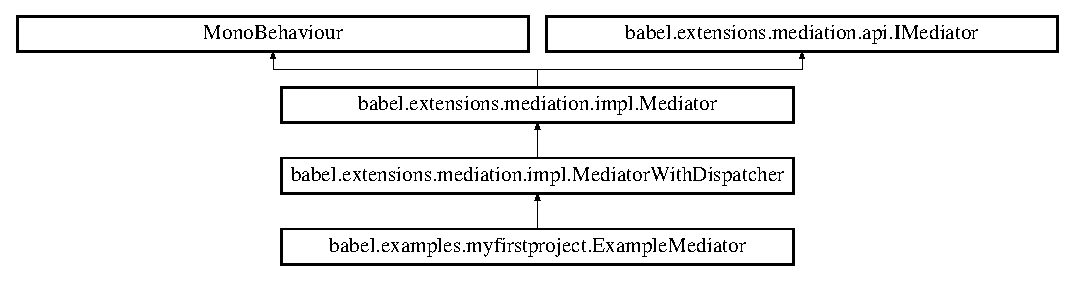
\includegraphics[height=3.333333cm]{classbabel_1_1examples_1_1myfirstproject_1_1_example_mediator}
\end{center}
\end{figure}
\subsection*{Public Member Functions}
\begin{DoxyCompactItemize}
\item 
override void \hyperlink{classbabel_1_1examples_1_1myfirstproject_1_1_example_mediator_abe56f9c8c8ab58eb281a27369b7e65b9}{on\-Register} ()
\begin{DoxyCompactList}\small\item\em Fires after all injections satisifed. \end{DoxyCompactList}\item 
override void \hyperlink{classbabel_1_1examples_1_1myfirstproject_1_1_example_mediator_ac6b3b96cc9b4e5532e7b34ed278eb1ac}{on\-Remove} ()
\begin{DoxyCompactList}\small\item\em Fires on removal of view. \end{DoxyCompactList}\end{DoxyCompactItemize}
\subsection*{Additional Inherited Members}


\subsection{Member Function Documentation}
\hypertarget{classbabel_1_1examples_1_1myfirstproject_1_1_example_mediator_abe56f9c8c8ab58eb281a27369b7e65b9}{\index{babel\-::examples\-::myfirstproject\-::\-Example\-Mediator@{babel\-::examples\-::myfirstproject\-::\-Example\-Mediator}!on\-Register@{on\-Register}}
\index{on\-Register@{on\-Register}!babel::examples::myfirstproject::ExampleMediator@{babel\-::examples\-::myfirstproject\-::\-Example\-Mediator}}
\subsubsection[{on\-Register}]{\setlength{\rightskip}{0pt plus 5cm}override void babel.\-examples.\-myfirstproject.\-Example\-Mediator.\-on\-Register (
\begin{DoxyParamCaption}
{}
\end{DoxyParamCaption}
)\hspace{0.3cm}{\ttfamily [inline]}, {\ttfamily [virtual]}}}\label{classbabel_1_1examples_1_1myfirstproject_1_1_example_mediator_abe56f9c8c8ab58eb281a27369b7e65b9}


Fires after all injections satisifed. 

Override and place your initialization code here. 

Reimplemented from \hyperlink{classbabel_1_1extensions_1_1mediation_1_1impl_1_1_mediator_a693800cf98ef09c660de249436108d9a}{babel.\-extensions.\-mediation.\-impl.\-Mediator}.

\hypertarget{classbabel_1_1examples_1_1myfirstproject_1_1_example_mediator_ac6b3b96cc9b4e5532e7b34ed278eb1ac}{\index{babel\-::examples\-::myfirstproject\-::\-Example\-Mediator@{babel\-::examples\-::myfirstproject\-::\-Example\-Mediator}!on\-Remove@{on\-Remove}}
\index{on\-Remove@{on\-Remove}!babel::examples::myfirstproject::ExampleMediator@{babel\-::examples\-::myfirstproject\-::\-Example\-Mediator}}
\subsubsection[{on\-Remove}]{\setlength{\rightskip}{0pt plus 5cm}override void babel.\-examples.\-myfirstproject.\-Example\-Mediator.\-on\-Remove (
\begin{DoxyParamCaption}
{}
\end{DoxyParamCaption}
)\hspace{0.3cm}{\ttfamily [inline]}, {\ttfamily [virtual]}}}\label{classbabel_1_1examples_1_1myfirstproject_1_1_example_mediator_ac6b3b96cc9b4e5532e7b34ed278eb1ac}


Fires on removal of view. 

Override and place your cleanup code here 

Reimplemented from \hyperlink{classbabel_1_1extensions_1_1mediation_1_1impl_1_1_mediator_a8b818665eda883eac66c83b8468007e9}{babel.\-extensions.\-mediation.\-impl.\-Mediator}.



The documentation for this class was generated from the following file\-:\begin{DoxyCompactItemize}
\item 
Assets/scripts/babel/examples/myfirstproject/view/Example\-Mediator.\-cs\end{DoxyCompactItemize}

\hypertarget{classbabel_1_1examples_1_1myfirstproject_1_1_example_model}{\section{babel.\-examples.\-myfirstproject.\-Example\-Model Class Reference}
\label{classbabel_1_1examples_1_1myfirstproject_1_1_example_model}\index{babel.\-examples.\-myfirstproject.\-Example\-Model@{babel.\-examples.\-myfirstproject.\-Example\-Model}}
}
Inheritance diagram for babel.\-examples.\-myfirstproject.\-Example\-Model\-:\begin{figure}[H]
\begin{center}
\leavevmode
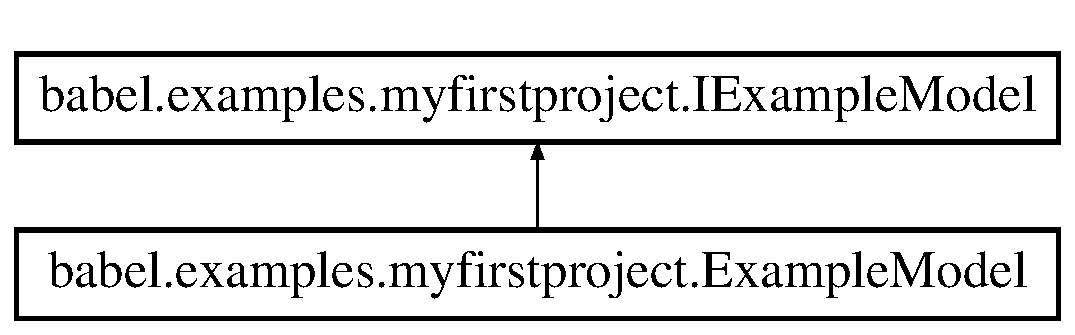
\includegraphics[height=2.000000cm]{classbabel_1_1examples_1_1myfirstproject_1_1_example_model}
\end{center}
\end{figure}
\subsection*{Properties}
\begin{DoxyCompactItemize}
\item 
\hypertarget{classbabel_1_1examples_1_1myfirstproject_1_1_example_model_a863e54bf05e702cf7f6deb3403da058e}{string {\bfseries data}\hspace{0.3cm}{\ttfamily  \mbox{[}get, set\mbox{]}}}\label{classbabel_1_1examples_1_1myfirstproject_1_1_example_model_a863e54bf05e702cf7f6deb3403da058e}

\end{DoxyCompactItemize}


The documentation for this class was generated from the following file\-:\begin{DoxyCompactItemize}
\item 
Assets/scripts/babel/examples/myfirstproject/model/Example\-Model.\-cs\end{DoxyCompactItemize}

\hypertarget{classbabel_1_1examples_1_1myfirstproject_1_1_example_service}{\section{babel.\-examples.\-myfirstproject.\-Example\-Service Class Reference}
\label{classbabel_1_1examples_1_1myfirstproject_1_1_example_service}\index{babel.\-examples.\-myfirstproject.\-Example\-Service@{babel.\-examples.\-myfirstproject.\-Example\-Service}}
}
Inheritance diagram for babel.\-examples.\-myfirstproject.\-Example\-Service\-:\begin{figure}[H]
\begin{center}
\leavevmode
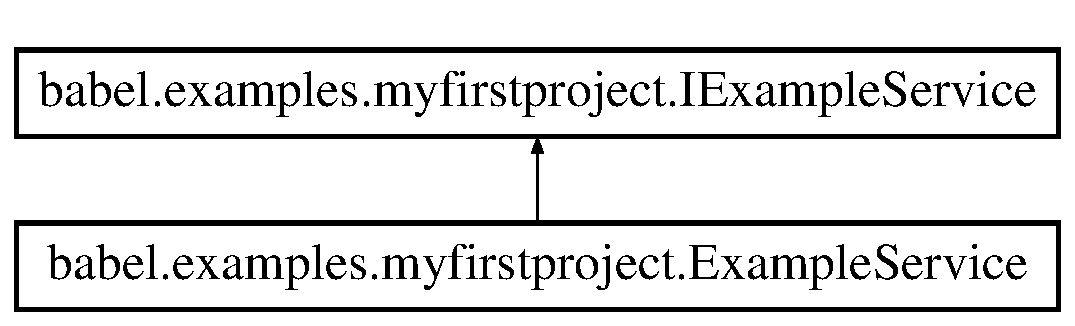
\includegraphics[height=2.000000cm]{classbabel_1_1examples_1_1myfirstproject_1_1_example_service}
\end{center}
\end{figure}
\subsection*{Public Member Functions}
\begin{DoxyCompactItemize}
\item 
\hypertarget{classbabel_1_1examples_1_1myfirstproject_1_1_example_service_a77f0b5a764b7323e8b63313ed7f5f1a1}{void {\bfseries Request} (string url)}\label{classbabel_1_1examples_1_1myfirstproject_1_1_example_service_a77f0b5a764b7323e8b63313ed7f5f1a1}

\end{DoxyCompactItemize}
\subsection*{Properties}
\begin{DoxyCompactItemize}
\item 
\hypertarget{classbabel_1_1examples_1_1myfirstproject_1_1_example_service_ad0b4836f8bc8c5adf6ce982b5711535c}{Game\-Object {\bfseries context\-View}\hspace{0.3cm}{\ttfamily  \mbox{[}get, set\mbox{]}}}\label{classbabel_1_1examples_1_1myfirstproject_1_1_example_service_ad0b4836f8bc8c5adf6ce982b5711535c}

\item 
\hypertarget{classbabel_1_1examples_1_1myfirstproject_1_1_example_service_a26136b8e477ec0c7470ac09fe54ddfae}{\hyperlink{interfacebabel_1_1extensions_1_1dispatcher_1_1eventdispatcher_1_1api_1_1_i_event_dispatcher}{I\-Event\-Dispatcher} {\bfseries dispatcher}\hspace{0.3cm}{\ttfamily  \mbox{[}get, set\mbox{]}}}\label{classbabel_1_1examples_1_1myfirstproject_1_1_example_service_a26136b8e477ec0c7470ac09fe54ddfae}

\end{DoxyCompactItemize}


The documentation for this class was generated from the following file\-:\begin{DoxyCompactItemize}
\item 
Assets/scripts/babel/examples/myfirstproject/service/Example\-Service.\-cs\end{DoxyCompactItemize}

\hypertarget{classbabel_1_1examples_1_1myfirstproject_1_1_example_view}{\section{babel.\-examples.\-myfirstproject.\-Example\-View Class Reference}
\label{classbabel_1_1examples_1_1myfirstproject_1_1_example_view}\index{babel.\-examples.\-myfirstproject.\-Example\-View@{babel.\-examples.\-myfirstproject.\-Example\-View}}
}
Inheritance diagram for babel.\-examples.\-myfirstproject.\-Example\-View\-:\begin{figure}[H]
\begin{center}
\leavevmode
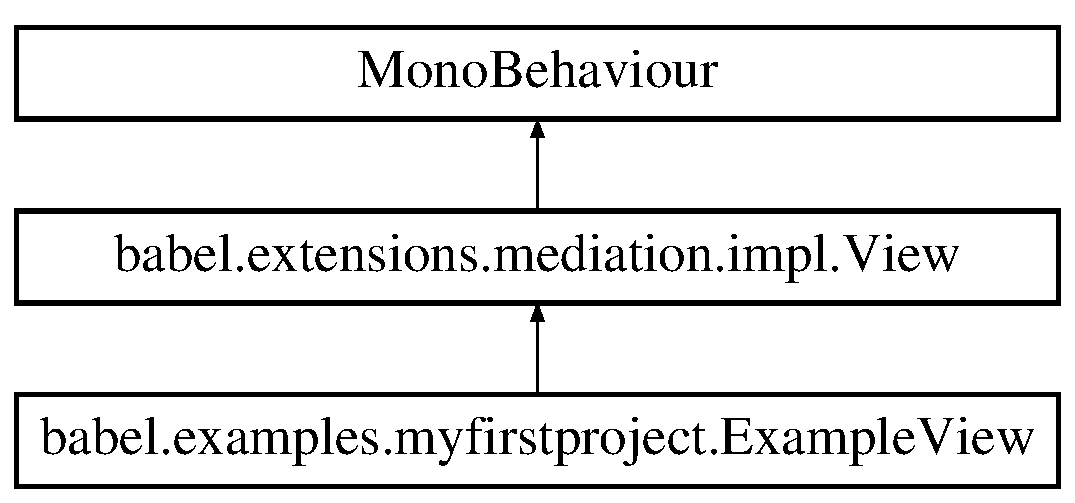
\includegraphics[height=3.000000cm]{classbabel_1_1examples_1_1myfirstproject_1_1_example_view}
\end{center}
\end{figure}
\subsection*{Public Attributes}
\begin{DoxyCompactItemize}
\item 
\hypertarget{classbabel_1_1examples_1_1myfirstproject_1_1_example_view_a39f263435cc239902f4df3e281accd5b}{float {\bfseries edx\-\_\-\-Wobble\-Size} = 1f}\label{classbabel_1_1examples_1_1myfirstproject_1_1_example_view_a39f263435cc239902f4df3e281accd5b}

\item 
\hypertarget{classbabel_1_1examples_1_1myfirstproject_1_1_example_view_a5f637a564c1af711b9ec29b2590d63ab}{float {\bfseries edx\-\_\-\-Wobble\-Dampen} = .\-9f}\label{classbabel_1_1examples_1_1myfirstproject_1_1_example_view_a5f637a564c1af711b9ec29b2590d63ab}

\item 
\hypertarget{classbabel_1_1examples_1_1myfirstproject_1_1_example_view_a81a76847f42b21be821101a179397a84}{float {\bfseries edx\-\_\-\-Wobble\-Min} = .\-001f}\label{classbabel_1_1examples_1_1myfirstproject_1_1_example_view_a81a76847f42b21be821101a179397a84}

\end{DoxyCompactItemize}
\subsection*{Properties}
\begin{DoxyCompactItemize}
\item 
\hypertarget{classbabel_1_1examples_1_1myfirstproject_1_1_example_view_a8071c6a62de597fa374387033013820c}{\hyperlink{interfacebabel_1_1extensions_1_1dispatcher_1_1eventdispatcher_1_1api_1_1_i_event_dispatcher}{I\-Event\-Dispatcher} {\bfseries dispatcher}\hspace{0.3cm}{\ttfamily  \mbox{[}get, set\mbox{]}}}\label{classbabel_1_1examples_1_1myfirstproject_1_1_example_view_a8071c6a62de597fa374387033013820c}

\end{DoxyCompactItemize}
\subsection*{Additional Inherited Members}


The documentation for this class was generated from the following file\-:\begin{DoxyCompactItemize}
\item 
Assets/scripts/babel/examples/myfirstproject/view/Example\-View.\-cs\end{DoxyCompactItemize}

\hypertarget{classbabel_1_1examples_1_1multiplecontexts_1_1social_1_1_facebook_service}{\section{babel.\-examples.\-multiplecontexts.\-social.\-Facebook\-Service Class Reference}
\label{classbabel_1_1examples_1_1multiplecontexts_1_1social_1_1_facebook_service}\index{babel.\-examples.\-multiplecontexts.\-social.\-Facebook\-Service@{babel.\-examples.\-multiplecontexts.\-social.\-Facebook\-Service}}
}
Inheritance diagram for babel.\-examples.\-multiplecontexts.\-social.\-Facebook\-Service\-:\begin{figure}[H]
\begin{center}
\leavevmode
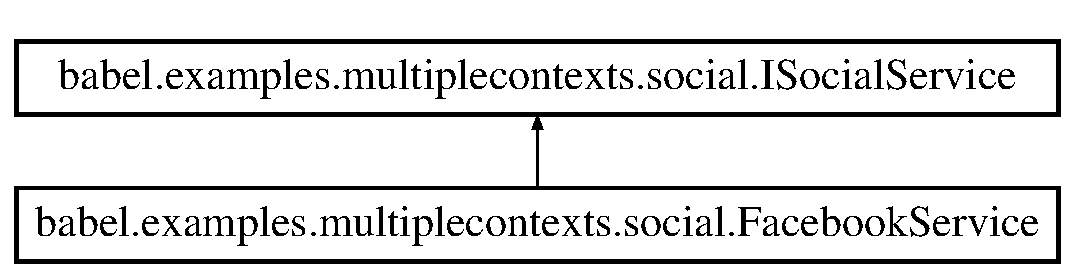
\includegraphics[height=2.000000cm]{classbabel_1_1examples_1_1multiplecontexts_1_1social_1_1_facebook_service}
\end{center}
\end{figure}
\subsection*{Public Member Functions}
\begin{DoxyCompactItemize}
\item 
\hypertarget{classbabel_1_1examples_1_1multiplecontexts_1_1social_1_1_facebook_service_a3370e9bada5f397b87a86c97b572cf0d}{void {\bfseries Fetch\-Current\-User} ()}\label{classbabel_1_1examples_1_1multiplecontexts_1_1social_1_1_facebook_service_a3370e9bada5f397b87a86c97b572cf0d}

\item 
\hypertarget{classbabel_1_1examples_1_1multiplecontexts_1_1social_1_1_facebook_service_a2fa3b7f9b81632f08d32729a85cb6293}{void {\bfseries Fetch\-Scores\-For\-Friends} ()}\label{classbabel_1_1examples_1_1multiplecontexts_1_1social_1_1_facebook_service_a2fa3b7f9b81632f08d32729a85cb6293}

\end{DoxyCompactItemize}
\subsection*{Properties}
\begin{DoxyCompactItemize}
\item 
\hypertarget{classbabel_1_1examples_1_1multiplecontexts_1_1social_1_1_facebook_service_aecaada0394e66b44f9b333e89804b406}{Game\-Object {\bfseries context\-View}\hspace{0.3cm}{\ttfamily  \mbox{[}get, set\mbox{]}}}\label{classbabel_1_1examples_1_1multiplecontexts_1_1social_1_1_facebook_service_aecaada0394e66b44f9b333e89804b406}

\item 
\hypertarget{classbabel_1_1examples_1_1multiplecontexts_1_1social_1_1_facebook_service_a9a4d1bc37ed4905a94f23cc3506f40d7}{\hyperlink{interfacebabel_1_1extensions_1_1dispatcher_1_1eventdispatcher_1_1api_1_1_i_event_dispatcher}{I\-Event\-Dispatcher} {\bfseries dispatcher}\hspace{0.3cm}{\ttfamily  \mbox{[}get, set\mbox{]}}}\label{classbabel_1_1examples_1_1multiplecontexts_1_1social_1_1_facebook_service_a9a4d1bc37ed4905a94f23cc3506f40d7}

\end{DoxyCompactItemize}


The documentation for this class was generated from the following file\-:\begin{DoxyCompactItemize}
\item 
Assets/scripts/babel/examples/multiplecontexts/social/service/Facebook\-Service.\-cs\end{DoxyCompactItemize}

\hypertarget{classbabel_1_1examples_1_1multiplecontexts_1_1main_1_1_game_complete_command}{\section{babel.\-examples.\-multiplecontexts.\-main.\-Game\-Complete\-Command Class Reference}
\label{classbabel_1_1examples_1_1multiplecontexts_1_1main_1_1_game_complete_command}\index{babel.\-examples.\-multiplecontexts.\-main.\-Game\-Complete\-Command@{babel.\-examples.\-multiplecontexts.\-main.\-Game\-Complete\-Command}}
}
Inheritance diagram for babel.\-examples.\-multiplecontexts.\-main.\-Game\-Complete\-Command\-:\begin{figure}[H]
\begin{center}
\leavevmode
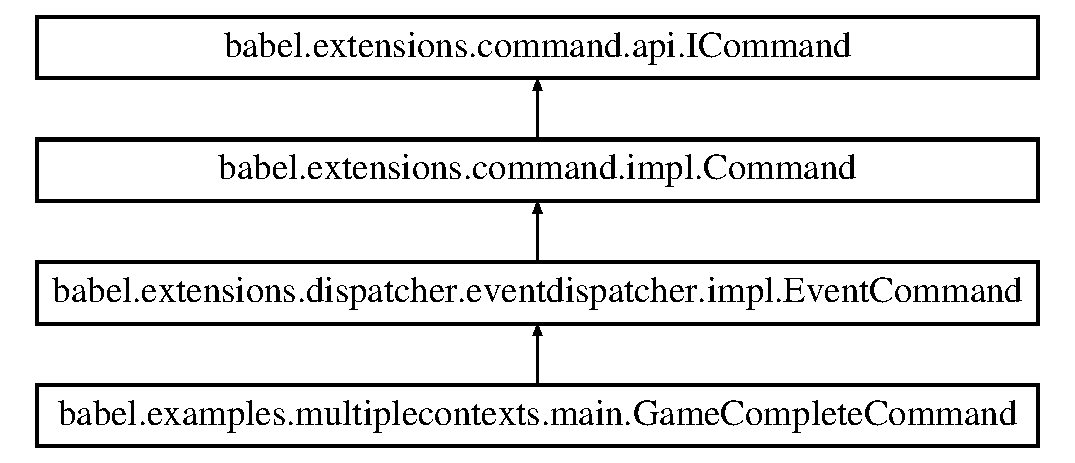
\includegraphics[height=4.000000cm]{classbabel_1_1examples_1_1multiplecontexts_1_1main_1_1_game_complete_command}
\end{center}
\end{figure}
\subsection*{Public Member Functions}
\begin{DoxyCompactItemize}
\item 
\hypertarget{classbabel_1_1examples_1_1multiplecontexts_1_1main_1_1_game_complete_command_a450e6a8bb8c5aebffef7c70b0ecca120}{override void {\bfseries Execute} ()}\label{classbabel_1_1examples_1_1multiplecontexts_1_1main_1_1_game_complete_command_a450e6a8bb8c5aebffef7c70b0ecca120}

\end{DoxyCompactItemize}
\subsection*{Properties}
\begin{DoxyCompactItemize}
\item 
\hypertarget{classbabel_1_1examples_1_1multiplecontexts_1_1main_1_1_game_complete_command_a0f191de11219b550ea4bd3ea9adcc979}{Game\-Object {\bfseries context\-View}\hspace{0.3cm}{\ttfamily  \mbox{[}get, set\mbox{]}}}\label{classbabel_1_1examples_1_1multiplecontexts_1_1main_1_1_game_complete_command_a0f191de11219b550ea4bd3ea9adcc979}

\end{DoxyCompactItemize}


The documentation for this class was generated from the following file\-:\begin{DoxyCompactItemize}
\item 
Assets/scripts/babel/examples/multiplecontexts/main/controller/Game\-Complete\-Command.\-cs\end{DoxyCompactItemize}

\hypertarget{classbabel_1_1examples_1_1multiplecontexts_1_1social_1_1_game_complete_command}{\section{babel.\-examples.\-multiplecontexts.\-social.\-Game\-Complete\-Command Class Reference}
\label{classbabel_1_1examples_1_1multiplecontexts_1_1social_1_1_game_complete_command}\index{babel.\-examples.\-multiplecontexts.\-social.\-Game\-Complete\-Command@{babel.\-examples.\-multiplecontexts.\-social.\-Game\-Complete\-Command}}
}
Inheritance diagram for babel.\-examples.\-multiplecontexts.\-social.\-Game\-Complete\-Command\-:\begin{figure}[H]
\begin{center}
\leavevmode
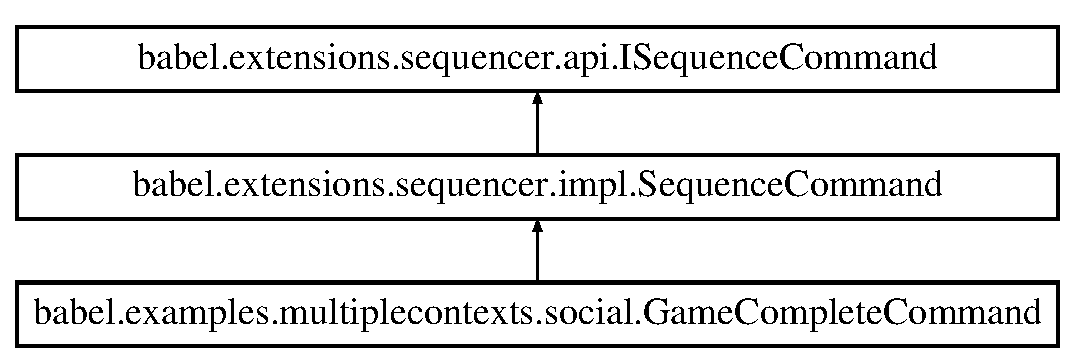
\includegraphics[height=3.000000cm]{classbabel_1_1examples_1_1multiplecontexts_1_1social_1_1_game_complete_command}
\end{center}
\end{figure}
\subsection*{Public Member Functions}
\begin{DoxyCompactItemize}
\item 
\hypertarget{classbabel_1_1examples_1_1multiplecontexts_1_1social_1_1_game_complete_command_a8d57db79fd40b42964429b6c3292c1ba}{override void {\bfseries Execute} ()}\label{classbabel_1_1examples_1_1multiplecontexts_1_1social_1_1_game_complete_command_a8d57db79fd40b42964429b6c3292c1ba}

\end{DoxyCompactItemize}
\subsection*{Properties}
\begin{DoxyCompactItemize}
\item 
\hypertarget{classbabel_1_1examples_1_1multiplecontexts_1_1social_1_1_game_complete_command_a5b407336659821a6582cd2cc5a97b469}{Game\-Object {\bfseries context\-View}\hspace{0.3cm}{\ttfamily  \mbox{[}get, set\mbox{]}}}\label{classbabel_1_1examples_1_1multiplecontexts_1_1social_1_1_game_complete_command_a5b407336659821a6582cd2cc5a97b469}

\item 
\hypertarget{classbabel_1_1examples_1_1multiplecontexts_1_1social_1_1_game_complete_command_a7042613531cd97a93d761390cae493ee}{\hyperlink{interfacebabel_1_1examples_1_1multiplecontexts_1_1social_1_1_i_social_service}{I\-Social\-Service} {\bfseries social}\hspace{0.3cm}{\ttfamily  \mbox{[}get, set\mbox{]}}}\label{classbabel_1_1examples_1_1multiplecontexts_1_1social_1_1_game_complete_command_a7042613531cd97a93d761390cae493ee}

\item 
\hypertarget{classbabel_1_1examples_1_1multiplecontexts_1_1social_1_1_game_complete_command_ac6e3d394c63ecdfefea8a8015e2dfcdc}{\hyperlink{classbabel_1_1examples_1_1multiplecontexts_1_1social_1_1_user_v_o}{User\-V\-O} {\bfseries user\-V\-O}\hspace{0.3cm}{\ttfamily  \mbox{[}get, set\mbox{]}}}\label{classbabel_1_1examples_1_1multiplecontexts_1_1social_1_1_game_complete_command_ac6e3d394c63ecdfefea8a8015e2dfcdc}

\end{DoxyCompactItemize}


The documentation for this class was generated from the following file\-:\begin{DoxyCompactItemize}
\item 
Assets/scripts/babel/examples/multiplecontexts/social/controller/Game\-Complete\-Command.\-cs\end{DoxyCompactItemize}

\hypertarget{classbabel_1_1examples_1_1multiplecontexts_1_1game_1_1_game_context}{\section{babel.\-examples.\-multiplecontexts.\-game.\-Game\-Context Class Reference}
\label{classbabel_1_1examples_1_1multiplecontexts_1_1game_1_1_game_context}\index{babel.\-examples.\-multiplecontexts.\-game.\-Game\-Context@{babel.\-examples.\-multiplecontexts.\-game.\-Game\-Context}}
}
Inheritance diagram for babel.\-examples.\-multiplecontexts.\-game.\-Game\-Context\-:\begin{figure}[H]
\begin{center}
\leavevmode
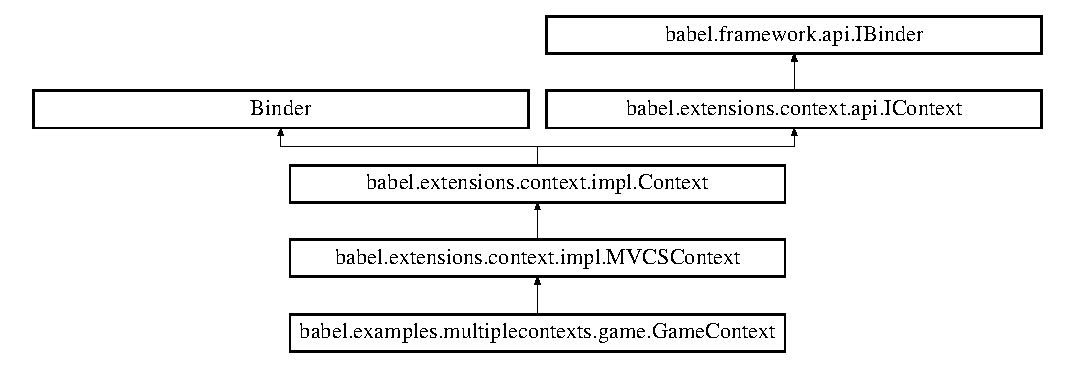
\includegraphics[height=4.501608cm]{classbabel_1_1examples_1_1multiplecontexts_1_1game_1_1_game_context}
\end{center}
\end{figure}
\subsection*{Public Member Functions}
\begin{DoxyCompactItemize}
\item 
\hypertarget{classbabel_1_1examples_1_1multiplecontexts_1_1game_1_1_game_context_a443098d2b9aabdd83b174b9f7e7925d0}{{\bfseries Game\-Context} (Mono\-Behaviour view, bool auto\-Startup)}\label{classbabel_1_1examples_1_1multiplecontexts_1_1game_1_1_game_context_a443098d2b9aabdd83b174b9f7e7925d0}

\end{DoxyCompactItemize}
\subsection*{Protected Member Functions}
\begin{DoxyCompactItemize}
\item 
\hypertarget{classbabel_1_1examples_1_1multiplecontexts_1_1game_1_1_game_context_a0935f6555370557a215330a3cd8d2e81}{override void {\bfseries map\-Bindings} ()}\label{classbabel_1_1examples_1_1multiplecontexts_1_1game_1_1_game_context_a0935f6555370557a215330a3cd8d2e81}

\end{DoxyCompactItemize}
\subsection*{Additional Inherited Members}


The documentation for this class was generated from the following file\-:\begin{DoxyCompactItemize}
\item 
Assets/scripts/babel/examples/multiplecontexts/game/Game\-Context.\-cs\end{DoxyCompactItemize}

\hypertarget{classbabel_1_1examples_1_1multiplecontexts_1_1game_1_1_game_event}{\section{babel.\-examples.\-multiplecontexts.\-game.\-Game\-Event Class Reference}
\label{classbabel_1_1examples_1_1multiplecontexts_1_1game_1_1_game_event}\index{babel.\-examples.\-multiplecontexts.\-game.\-Game\-Event@{babel.\-examples.\-multiplecontexts.\-game.\-Game\-Event}}
}
\subsection*{Public Attributes}
\begin{DoxyCompactItemize}
\item 
\hypertarget{classbabel_1_1examples_1_1multiplecontexts_1_1game_1_1_game_event_a7ce173398d9bf2ba9b23d89925fe611a}{const string {\bfseries A\-D\-D\-\_\-\-T\-O\-\_\-\-S\-C\-O\-R\-E} = \char`\"{}A\-D\-D\-\_\-\-T\-O\-\_\-\-S\-C\-O\-R\-E\char`\"{}}\label{classbabel_1_1examples_1_1multiplecontexts_1_1game_1_1_game_event_a7ce173398d9bf2ba9b23d89925fe611a}

\item 
\hypertarget{classbabel_1_1examples_1_1multiplecontexts_1_1game_1_1_game_event_a5f84dc8a5ebc96c32cde1bd7f1c1077f}{const string {\bfseries G\-A\-M\-E\-\_\-\-O\-V\-E\-R} = \char`\"{}G\-A\-M\-E\-\_\-\-O\-V\-E\-R\char`\"{}}\label{classbabel_1_1examples_1_1multiplecontexts_1_1game_1_1_game_event_a5f84dc8a5ebc96c32cde1bd7f1c1077f}

\item 
\hypertarget{classbabel_1_1examples_1_1multiplecontexts_1_1game_1_1_game_event_a930302a30e31f2ef6744d60aa3d9f760}{const string {\bfseries G\-A\-M\-E\-\_\-\-U\-P\-D\-A\-T\-E} = \char`\"{}G\-A\-M\-E\-\_\-\-U\-P\-D\-A\-T\-E\char`\"{}}\label{classbabel_1_1examples_1_1multiplecontexts_1_1game_1_1_game_event_a930302a30e31f2ef6744d60aa3d9f760}

\item 
\hypertarget{classbabel_1_1examples_1_1multiplecontexts_1_1game_1_1_game_event_a4bb75ca19708f400cf0644b576fd1d73}{const string {\bfseries L\-I\-V\-E\-S\-\_\-\-C\-H\-A\-N\-G\-E} = \char`\"{}L\-I\-V\-E\-S\-\_\-\-C\-H\-A\-N\-G\-E\char`\"{}}\label{classbabel_1_1examples_1_1multiplecontexts_1_1game_1_1_game_event_a4bb75ca19708f400cf0644b576fd1d73}

\item 
\hypertarget{classbabel_1_1examples_1_1multiplecontexts_1_1game_1_1_game_event_a38793c4dfddcef400a8a42bf4f5c4395}{const string {\bfseries R\-E\-P\-L\-A\-Y} = \char`\"{}R\-E\-P\-L\-A\-Y\-\_\-\-R\-E\-Q\-U\-E\-S\-T\char`\"{}}\label{classbabel_1_1examples_1_1multiplecontexts_1_1game_1_1_game_event_a38793c4dfddcef400a8a42bf4f5c4395}

\item 
\hypertarget{classbabel_1_1examples_1_1multiplecontexts_1_1game_1_1_game_event_a8c93ce3329746418d4e81770274f03d9}{const string {\bfseries R\-E\-S\-T\-A\-R\-T\-\_\-\-G\-A\-M\-E} = \char`\"{}R\-E\-S\-T\-A\-R\-T\-\_\-\-G\-A\-M\-E\char`\"{}}\label{classbabel_1_1examples_1_1multiplecontexts_1_1game_1_1_game_event_a8c93ce3329746418d4e81770274f03d9}

\item 
\hypertarget{classbabel_1_1examples_1_1multiplecontexts_1_1game_1_1_game_event_a13d8e45a7e0ec28ed4b5f414c3c5dad7}{const string {\bfseries S\-C\-O\-R\-E\-\_\-\-C\-H\-A\-N\-G\-E} = \char`\"{}S\-C\-O\-R\-E\-\_\-\-C\-H\-A\-N\-G\-E\char`\"{}}\label{classbabel_1_1examples_1_1multiplecontexts_1_1game_1_1_game_event_a13d8e45a7e0ec28ed4b5f414c3c5dad7}

\item 
\hypertarget{classbabel_1_1examples_1_1multiplecontexts_1_1game_1_1_game_event_af2436dd0a75d181307d6f58be278619c}{const string {\bfseries S\-H\-I\-P\-\_\-\-D\-E\-S\-T\-R\-O\-Y\-E\-D} = \char`\"{}S\-H\-I\-P\-\_\-\-D\-E\-S\-T\-R\-O\-Y\-E\-D\char`\"{}}\label{classbabel_1_1examples_1_1multiplecontexts_1_1game_1_1_game_event_af2436dd0a75d181307d6f58be278619c}

\end{DoxyCompactItemize}


The documentation for this class was generated from the following file\-:\begin{DoxyCompactItemize}
\item 
Assets/scripts/babel/examples/multiplecontexts/game/controller/Game\-Event.\-cs\end{DoxyCompactItemize}

\hypertarget{classbabel_1_1examples_1_1multiplecontexts_1_1game_1_1_game_loop}{\section{babel.\-examples.\-multiplecontexts.\-game.\-Game\-Loop Class Reference}
\label{classbabel_1_1examples_1_1multiplecontexts_1_1game_1_1_game_loop}\index{babel.\-examples.\-multiplecontexts.\-game.\-Game\-Loop@{babel.\-examples.\-multiplecontexts.\-game.\-Game\-Loop}}
}
Inheritance diagram for babel.\-examples.\-multiplecontexts.\-game.\-Game\-Loop\-:\begin{figure}[H]
\begin{center}
\leavevmode
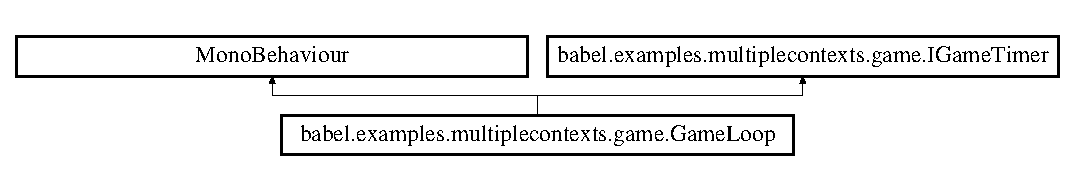
\includegraphics[height=1.848185cm]{classbabel_1_1examples_1_1multiplecontexts_1_1game_1_1_game_loop}
\end{center}
\end{figure}
\subsection*{Public Member Functions}
\begin{DoxyCompactItemize}
\item 
\hypertarget{classbabel_1_1examples_1_1multiplecontexts_1_1game_1_1_game_loop_a3991ff15c6602d5f8f22702135a52903}{void {\bfseries Start} ()}\label{classbabel_1_1examples_1_1multiplecontexts_1_1game_1_1_game_loop_a3991ff15c6602d5f8f22702135a52903}

\item 
\hypertarget{classbabel_1_1examples_1_1multiplecontexts_1_1game_1_1_game_loop_a9539ae66df3fe208b7fd156a6036d88a}{void {\bfseries Stop} ()}\label{classbabel_1_1examples_1_1multiplecontexts_1_1game_1_1_game_loop_a9539ae66df3fe208b7fd156a6036d88a}

\end{DoxyCompactItemize}
\subsection*{Properties}
\begin{DoxyCompactItemize}
\item 
\hypertarget{classbabel_1_1examples_1_1multiplecontexts_1_1game_1_1_game_loop_adbad8554b6b2a15c52ac1098677b940f}{\hyperlink{interfacebabel_1_1extensions_1_1dispatcher_1_1eventdispatcher_1_1api_1_1_i_event_dispatcher}{I\-Event\-Dispatcher} {\bfseries dispatcher}\hspace{0.3cm}{\ttfamily  \mbox{[}get, set\mbox{]}}}\label{classbabel_1_1examples_1_1multiplecontexts_1_1game_1_1_game_loop_adbad8554b6b2a15c52ac1098677b940f}

\end{DoxyCompactItemize}


The documentation for this class was generated from the following file\-:\begin{DoxyCompactItemize}
\item 
Assets/scripts/babel/examples/multiplecontexts/game/util/Game\-Loop.\-cs\end{DoxyCompactItemize}

\hypertarget{classbabel_1_1examples_1_1multiplecontexts_1_1game_1_1_game_over_command}{\section{babel.\-examples.\-multiplecontexts.\-game.\-Game\-Over\-Command Class Reference}
\label{classbabel_1_1examples_1_1multiplecontexts_1_1game_1_1_game_over_command}\index{babel.\-examples.\-multiplecontexts.\-game.\-Game\-Over\-Command@{babel.\-examples.\-multiplecontexts.\-game.\-Game\-Over\-Command}}
}
Inheritance diagram for babel.\-examples.\-multiplecontexts.\-game.\-Game\-Over\-Command\-:\begin{figure}[H]
\begin{center}
\leavevmode
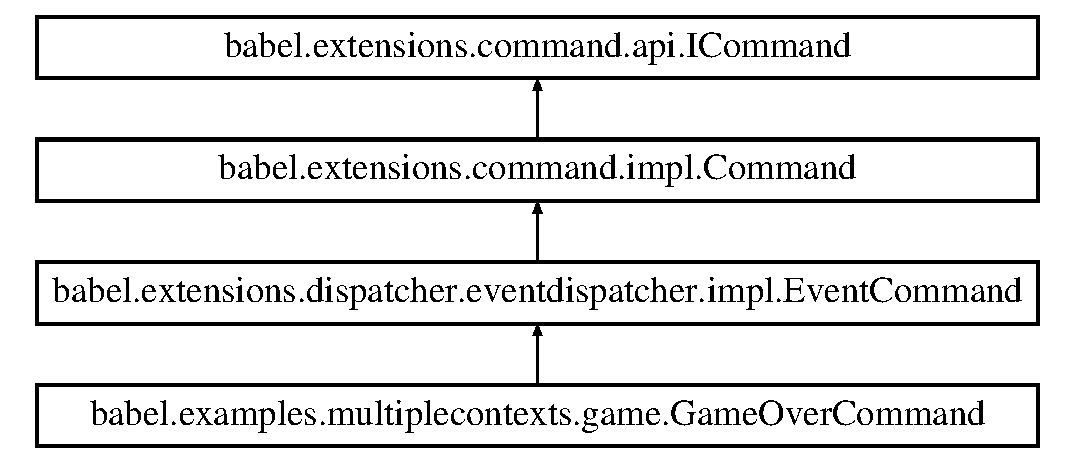
\includegraphics[height=4.000000cm]{classbabel_1_1examples_1_1multiplecontexts_1_1game_1_1_game_over_command}
\end{center}
\end{figure}
\subsection*{Public Member Functions}
\begin{DoxyCompactItemize}
\item 
\hypertarget{classbabel_1_1examples_1_1multiplecontexts_1_1game_1_1_game_over_command_af18bdf53aef3ee5c29a2467d78c67fea}{override void {\bfseries Execute} ()}\label{classbabel_1_1examples_1_1multiplecontexts_1_1game_1_1_game_over_command_af18bdf53aef3ee5c29a2467d78c67fea}

\end{DoxyCompactItemize}
\subsection*{Properties}
\begin{DoxyCompactItemize}
\item 
\hypertarget{classbabel_1_1examples_1_1multiplecontexts_1_1game_1_1_game_over_command_ac4ef3ae2a30e67724b254e5605d0b05d}{\hyperlink{interfacebabel_1_1examples_1_1multiplecontexts_1_1game_1_1_i_score}{I\-Score} {\bfseries score\-Keeper}\hspace{0.3cm}{\ttfamily  \mbox{[}get, set\mbox{]}}}\label{classbabel_1_1examples_1_1multiplecontexts_1_1game_1_1_game_over_command_ac4ef3ae2a30e67724b254e5605d0b05d}

\item 
\hypertarget{classbabel_1_1examples_1_1multiplecontexts_1_1game_1_1_game_over_command_a75ae5f7138460cfd416411f0b3bab583}{\hyperlink{interfacebabel_1_1examples_1_1multiplecontexts_1_1game_1_1_i_game_timer}{I\-Game\-Timer} {\bfseries game\-Timer}\hspace{0.3cm}{\ttfamily  \mbox{[}get, set\mbox{]}}}\label{classbabel_1_1examples_1_1multiplecontexts_1_1game_1_1_game_over_command_a75ae5f7138460cfd416411f0b3bab583}

\item 
\hypertarget{classbabel_1_1examples_1_1multiplecontexts_1_1game_1_1_game_over_command_a6bfa01211d8c9b18f038c1c661af380c}{\hyperlink{interfacebabel_1_1extensions_1_1dispatcher_1_1eventdispatcher_1_1api_1_1_i_event_dispatcher}{I\-Event\-Dispatcher} {\bfseries cross\-Context\-Dispatcher}\hspace{0.3cm}{\ttfamily  \mbox{[}get, set\mbox{]}}}\label{classbabel_1_1examples_1_1multiplecontexts_1_1game_1_1_game_over_command_a6bfa01211d8c9b18f038c1c661af380c}

\end{DoxyCompactItemize}


The documentation for this class was generated from the following file\-:\begin{DoxyCompactItemize}
\item 
Assets/scripts/babel/examples/multiplecontexts/game/controller/Game\-Over\-Command.\-cs\end{DoxyCompactItemize}

\hypertarget{classbabel_1_1examples_1_1multiplecontexts_1_1game_1_1_game_root}{\section{babel.\-examples.\-multiplecontexts.\-game.\-Game\-Root Class Reference}
\label{classbabel_1_1examples_1_1multiplecontexts_1_1game_1_1_game_root}\index{babel.\-examples.\-multiplecontexts.\-game.\-Game\-Root@{babel.\-examples.\-multiplecontexts.\-game.\-Game\-Root}}
}
Inheritance diagram for babel.\-examples.\-multiplecontexts.\-game.\-Game\-Root\-:\begin{figure}[H]
\begin{center}
\leavevmode
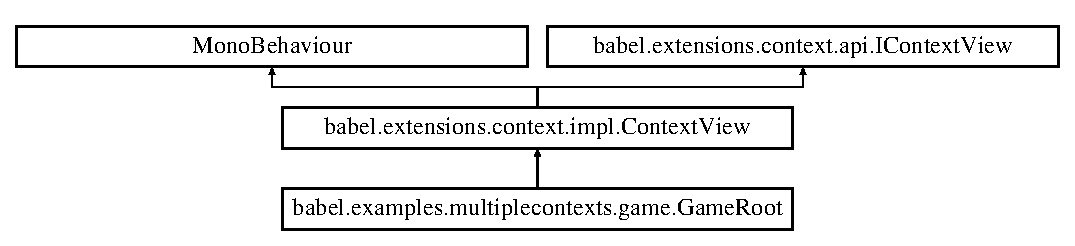
\includegraphics[height=2.857143cm]{classbabel_1_1examples_1_1multiplecontexts_1_1game_1_1_game_root}
\end{center}
\end{figure}
\subsection*{Additional Inherited Members}


The documentation for this class was generated from the following file\-:\begin{DoxyCompactItemize}
\item 
Assets/scripts/babel/examples/multiplecontexts/game/Game\-Root.\-cs\end{DoxyCompactItemize}

\hypertarget{classbabel_1_1examples_1_1multiplecontexts_1_1social_1_1_google_service}{\section{babel.\-examples.\-multiplecontexts.\-social.\-Google\-Service Class Reference}
\label{classbabel_1_1examples_1_1multiplecontexts_1_1social_1_1_google_service}\index{babel.\-examples.\-multiplecontexts.\-social.\-Google\-Service@{babel.\-examples.\-multiplecontexts.\-social.\-Google\-Service}}
}
Inheritance diagram for babel.\-examples.\-multiplecontexts.\-social.\-Google\-Service\-:\begin{figure}[H]
\begin{center}
\leavevmode
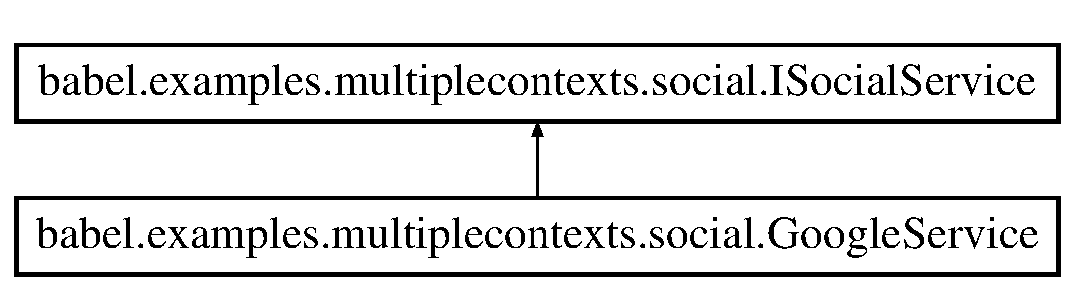
\includegraphics[height=2.000000cm]{classbabel_1_1examples_1_1multiplecontexts_1_1social_1_1_google_service}
\end{center}
\end{figure}
\subsection*{Public Member Functions}
\begin{DoxyCompactItemize}
\item 
\hypertarget{classbabel_1_1examples_1_1multiplecontexts_1_1social_1_1_google_service_ae4dab2cf63225a8727fbb44d73331d29}{void {\bfseries Fetch\-Current\-User} ()}\label{classbabel_1_1examples_1_1multiplecontexts_1_1social_1_1_google_service_ae4dab2cf63225a8727fbb44d73331d29}

\item 
\hypertarget{classbabel_1_1examples_1_1multiplecontexts_1_1social_1_1_google_service_a109313b37c86a26306769e597bc02780}{void {\bfseries Fetch\-Scores\-For\-Friends} ()}\label{classbabel_1_1examples_1_1multiplecontexts_1_1social_1_1_google_service_a109313b37c86a26306769e597bc02780}

\end{DoxyCompactItemize}
\subsection*{Properties}
\begin{DoxyCompactItemize}
\item 
\hypertarget{classbabel_1_1examples_1_1multiplecontexts_1_1social_1_1_google_service_a1d9ea1a31f0f341d2c85d2ffea2ef5ef}{Game\-Object {\bfseries context\-View}\hspace{0.3cm}{\ttfamily  \mbox{[}get, set\mbox{]}}}\label{classbabel_1_1examples_1_1multiplecontexts_1_1social_1_1_google_service_a1d9ea1a31f0f341d2c85d2ffea2ef5ef}

\item 
\hypertarget{classbabel_1_1examples_1_1multiplecontexts_1_1social_1_1_google_service_ac69466caf61dcc62fe8c41996a704a1a}{\hyperlink{interfacebabel_1_1extensions_1_1dispatcher_1_1eventdispatcher_1_1api_1_1_i_event_dispatcher}{I\-Event\-Dispatcher} {\bfseries dispatcher}\hspace{0.3cm}{\ttfamily  \mbox{[}get, set\mbox{]}}}\label{classbabel_1_1examples_1_1multiplecontexts_1_1social_1_1_google_service_ac69466caf61dcc62fe8c41996a704a1a}

\end{DoxyCompactItemize}


The documentation for this class was generated from the following file\-:\begin{DoxyCompactItemize}
\item 
Assets/scripts/babel/examples/multiplecontexts/social/service/Google\-Service.\-cs\end{DoxyCompactItemize}

\hypertarget{interfacebabel_1_1framework_1_1api_1_1_i_binder}{\section{babel.\-framework.\-api.\-I\-Binder Interface Reference}
\label{interfacebabel_1_1framework_1_1api_1_1_i_binder}\index{babel.\-framework.\-api.\-I\-Binder@{babel.\-framework.\-api.\-I\-Binder}}
}
Inheritance diagram for babel.\-framework.\-api.\-I\-Binder\-:\begin{figure}[H]
\begin{center}
\leavevmode
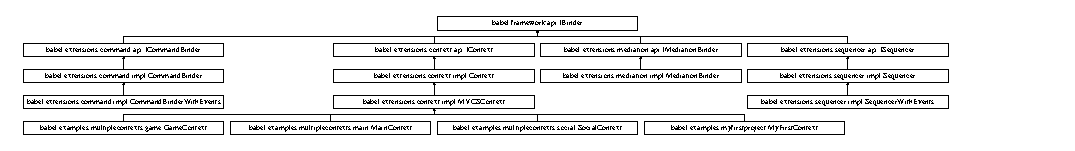
\includegraphics[height=1.577465cm]{interfacebabel_1_1framework_1_1api_1_1_i_binder}
\end{center}
\end{figure}
\subsection*{Public Member Functions}
\begin{DoxyCompactItemize}
\item 
\hypertarget{interfacebabel_1_1framework_1_1api_1_1_i_binder_a3c7c6f04355ef9acd7599a71714fc53a}{\hyperlink{interfacebabel_1_1framework_1_1api_1_1_i_binding}{I\-Binding} {\bfseries Bind$<$ T $>$} ()}\label{interfacebabel_1_1framework_1_1api_1_1_i_binder_a3c7c6f04355ef9acd7599a71714fc53a}

\item 
\hypertarget{interfacebabel_1_1framework_1_1api_1_1_i_binder_ad426acf94c6ca385d72775bf09639dbc}{\hyperlink{interfacebabel_1_1framework_1_1api_1_1_i_binding}{I\-Binding} {\bfseries Bind} (object value)}\label{interfacebabel_1_1framework_1_1api_1_1_i_binder_ad426acf94c6ca385d72775bf09639dbc}

\item 
\hypertarget{interfacebabel_1_1framework_1_1api_1_1_i_binder_a6ac453f0d36164498e05f533496444cb}{\hyperlink{interfacebabel_1_1framework_1_1api_1_1_i_binding}{I\-Binding} {\bfseries Get\-Binding$<$ T $>$} ()}\label{interfacebabel_1_1framework_1_1api_1_1_i_binder_a6ac453f0d36164498e05f533496444cb}

\item 
\hypertarget{interfacebabel_1_1framework_1_1api_1_1_i_binder_a62777b1cd7d45309a1c40d74684e36f8}{\hyperlink{interfacebabel_1_1framework_1_1api_1_1_i_binding}{I\-Binding} {\bfseries Get\-Binding} (object key)}\label{interfacebabel_1_1framework_1_1api_1_1_i_binder_a62777b1cd7d45309a1c40d74684e36f8}

\item 
\hypertarget{interfacebabel_1_1framework_1_1api_1_1_i_binder_a9139f355714981b1c23a344380883374}{\hyperlink{interfacebabel_1_1framework_1_1api_1_1_i_binding}{I\-Binding} {\bfseries Get\-Binding$<$ T $>$} (object name)}\label{interfacebabel_1_1framework_1_1api_1_1_i_binder_a9139f355714981b1c23a344380883374}

\item 
\hypertarget{interfacebabel_1_1framework_1_1api_1_1_i_binder_a9ea4cc1ba3d419b70b3e2be3d77a2d1a}{\hyperlink{interfacebabel_1_1framework_1_1api_1_1_i_binding}{I\-Binding} {\bfseries Get\-Binding} (object key, object name)}\label{interfacebabel_1_1framework_1_1api_1_1_i_binder_a9ea4cc1ba3d419b70b3e2be3d77a2d1a}

\item 
\hypertarget{interfacebabel_1_1framework_1_1api_1_1_i_binder_a5fe3c62f4de7dd36747ea97037005aed}{\hyperlink{interfacebabel_1_1framework_1_1api_1_1_i_binding}{I\-Binding} {\bfseries Get\-Raw\-Binding} ()}\label{interfacebabel_1_1framework_1_1api_1_1_i_binder_a5fe3c62f4de7dd36747ea97037005aed}

\item 
\hypertarget{interfacebabel_1_1framework_1_1api_1_1_i_binder_a916a0bfef185d1529f1370a79a585bb4}{void {\bfseries Unbind$<$ T $>$} ()}\label{interfacebabel_1_1framework_1_1api_1_1_i_binder_a916a0bfef185d1529f1370a79a585bb4}

\item 
\hypertarget{interfacebabel_1_1framework_1_1api_1_1_i_binder_adff747fb13c6fcbc76cb9c4d0c935a4c}{void {\bfseries Unbind$<$ T $>$} (object name)}\label{interfacebabel_1_1framework_1_1api_1_1_i_binder_adff747fb13c6fcbc76cb9c4d0c935a4c}

\item 
\hypertarget{interfacebabel_1_1framework_1_1api_1_1_i_binder_a7fbc00de4ee1a24f6ff3a1e01d658a19}{void {\bfseries Unbind} (object key)}\label{interfacebabel_1_1framework_1_1api_1_1_i_binder_a7fbc00de4ee1a24f6ff3a1e01d658a19}

\item 
\hypertarget{interfacebabel_1_1framework_1_1api_1_1_i_binder_ad925c5544e63e3c198551a4c76882aba}{void {\bfseries Unbind} (object key, object name)}\label{interfacebabel_1_1framework_1_1api_1_1_i_binder_ad925c5544e63e3c198551a4c76882aba}

\item 
\hypertarget{interfacebabel_1_1framework_1_1api_1_1_i_binder_a6eaf1663ce098a9f3abbf3182435f44b}{void {\bfseries Unbind} (\hyperlink{interfacebabel_1_1framework_1_1api_1_1_i_binding}{I\-Binding} binding)}\label{interfacebabel_1_1framework_1_1api_1_1_i_binder_a6eaf1663ce098a9f3abbf3182435f44b}

\item 
\hypertarget{interfacebabel_1_1framework_1_1api_1_1_i_binder_ac474d26468af6703dd1a55c96a918746}{void {\bfseries Remove\-Value} (\hyperlink{interfacebabel_1_1framework_1_1api_1_1_i_binding}{I\-Binding} binding, object value)}\label{interfacebabel_1_1framework_1_1api_1_1_i_binder_ac474d26468af6703dd1a55c96a918746}

\item 
\hypertarget{interfacebabel_1_1framework_1_1api_1_1_i_binder_a7f85832b11bb771bd1d6ec043bce2d27}{void {\bfseries Remove\-Key} (\hyperlink{interfacebabel_1_1framework_1_1api_1_1_i_binding}{I\-Binding} binding, object value)}\label{interfacebabel_1_1framework_1_1api_1_1_i_binder_a7f85832b11bb771bd1d6ec043bce2d27}

\item 
\hypertarget{interfacebabel_1_1framework_1_1api_1_1_i_binder_aa0e2406e6803718e463095a807cbd525}{void {\bfseries Remove\-Name} (\hyperlink{interfacebabel_1_1framework_1_1api_1_1_i_binding}{I\-Binding} binding, object value)}\label{interfacebabel_1_1framework_1_1api_1_1_i_binder_aa0e2406e6803718e463095a807cbd525}

\end{DoxyCompactItemize}


The documentation for this interface was generated from the following file\-:\begin{DoxyCompactItemize}
\item 
Assets/scripts/babel/framework/api/I\-Binder.\-cs\end{DoxyCompactItemize}

\hypertarget{interfacebabel_1_1framework_1_1api_1_1_i_binding}{\section{babel.\-framework.\-api.\-I\-Binding Interface Reference}
\label{interfacebabel_1_1framework_1_1api_1_1_i_binding}\index{babel.\-framework.\-api.\-I\-Binding@{babel.\-framework.\-api.\-I\-Binding}}
}
Inheritance diagram for babel.\-framework.\-api.\-I\-Binding\-:\begin{figure}[H]
\begin{center}
\leavevmode
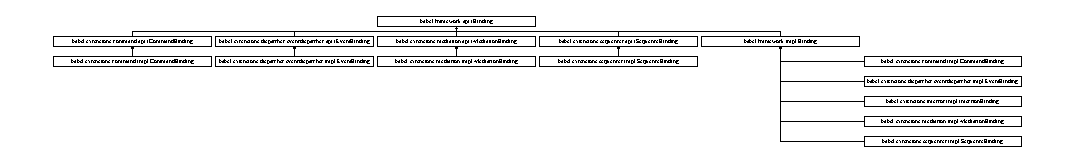
\includegraphics[height=1.742222cm]{interfacebabel_1_1framework_1_1api_1_1_i_binding}
\end{center}
\end{figure}
\subsection*{Public Member Functions}
\begin{DoxyCompactItemize}
\item 
\hypertarget{interfacebabel_1_1framework_1_1api_1_1_i_binding_aa34c9708eb5511fe163f1673bbe56542}{\hyperlink{interfacebabel_1_1framework_1_1api_1_1_i_binding}{I\-Binding} {\bfseries Key$<$ T $>$} ()}\label{interfacebabel_1_1framework_1_1api_1_1_i_binding_aa34c9708eb5511fe163f1673bbe56542}

\item 
\hypertarget{interfacebabel_1_1framework_1_1api_1_1_i_binding_a10e727cc324ee02d8faa03e3ae9541c2}{\hyperlink{interfacebabel_1_1framework_1_1api_1_1_i_binding}{I\-Binding} {\bfseries Key} (object key)}\label{interfacebabel_1_1framework_1_1api_1_1_i_binding_a10e727cc324ee02d8faa03e3ae9541c2}

\item 
\hypertarget{interfacebabel_1_1framework_1_1api_1_1_i_binding_a62609c8016c9c556450b4c11e88212a4}{\hyperlink{interfacebabel_1_1framework_1_1api_1_1_i_binding}{I\-Binding} {\bfseries To$<$ T $>$} ()}\label{interfacebabel_1_1framework_1_1api_1_1_i_binding_a62609c8016c9c556450b4c11e88212a4}

\item 
\hypertarget{interfacebabel_1_1framework_1_1api_1_1_i_binding_a997567dab2e1fba2e63785aa9c4a62c3}{\hyperlink{interfacebabel_1_1framework_1_1api_1_1_i_binding}{I\-Binding} {\bfseries To} (object o)}\label{interfacebabel_1_1framework_1_1api_1_1_i_binding_a997567dab2e1fba2e63785aa9c4a62c3}

\item 
\hypertarget{interfacebabel_1_1framework_1_1api_1_1_i_binding_a5e07e79d02ea1c2c5e64c217562d8e14}{\hyperlink{interfacebabel_1_1framework_1_1api_1_1_i_binding}{I\-Binding} {\bfseries To\-Name$<$ T $>$} ()}\label{interfacebabel_1_1framework_1_1api_1_1_i_binding_a5e07e79d02ea1c2c5e64c217562d8e14}

\item 
\hypertarget{interfacebabel_1_1framework_1_1api_1_1_i_binding_af8483c35725135b842a45afd7084a820}{\hyperlink{interfacebabel_1_1framework_1_1api_1_1_i_binding}{I\-Binding} {\bfseries To\-Name} (object o)}\label{interfacebabel_1_1framework_1_1api_1_1_i_binding_af8483c35725135b842a45afd7084a820}

\item 
\hypertarget{interfacebabel_1_1framework_1_1api_1_1_i_binding_a723a2166ac506fdf1383bffe76e4f246}{\hyperlink{interfacebabel_1_1framework_1_1api_1_1_i_binding}{I\-Binding} {\bfseries Named$<$ T $>$} ()}\label{interfacebabel_1_1framework_1_1api_1_1_i_binding_a723a2166ac506fdf1383bffe76e4f246}

\item 
\hypertarget{interfacebabel_1_1framework_1_1api_1_1_i_binding_a4bd1c5fda531020e7f27447f20c9fb1e}{\hyperlink{interfacebabel_1_1framework_1_1api_1_1_i_binding}{I\-Binding} {\bfseries Named} (object o)}\label{interfacebabel_1_1framework_1_1api_1_1_i_binding_a4bd1c5fda531020e7f27447f20c9fb1e}

\item 
\hypertarget{interfacebabel_1_1framework_1_1api_1_1_i_binding_a1ddb463b1d9abd4049af67ffad90425c}{void {\bfseries Remove\-Key} (object o)}\label{interfacebabel_1_1framework_1_1api_1_1_i_binding_a1ddb463b1d9abd4049af67ffad90425c}

\item 
\hypertarget{interfacebabel_1_1framework_1_1api_1_1_i_binding_a23b5a522bc89039a1610006745d0b153}{void {\bfseries Remove\-Value} (object o)}\label{interfacebabel_1_1framework_1_1api_1_1_i_binding_a23b5a522bc89039a1610006745d0b153}

\item 
\hypertarget{interfacebabel_1_1framework_1_1api_1_1_i_binding_a837204d72a5c59aefd7e3a57b1880252}{void {\bfseries Remove\-Name} (object o)}\label{interfacebabel_1_1framework_1_1api_1_1_i_binding_a837204d72a5c59aefd7e3a57b1880252}

\end{DoxyCompactItemize}
\subsection*{Properties}
\begin{DoxyCompactItemize}
\item 
\hypertarget{interfacebabel_1_1framework_1_1api_1_1_i_binding_ac57df2a0c37244d530329377358177e8}{object {\bfseries key}\hspace{0.3cm}{\ttfamily  \mbox{[}get\mbox{]}}}\label{interfacebabel_1_1framework_1_1api_1_1_i_binding_ac57df2a0c37244d530329377358177e8}

\item 
\hypertarget{interfacebabel_1_1framework_1_1api_1_1_i_binding_accc7009d33b5ff0f8f6b39351fb17122}{object {\bfseries name}\hspace{0.3cm}{\ttfamily  \mbox{[}get\mbox{]}}}\label{interfacebabel_1_1framework_1_1api_1_1_i_binding_accc7009d33b5ff0f8f6b39351fb17122}

\item 
\hypertarget{interfacebabel_1_1framework_1_1api_1_1_i_binding_abe764979414f9f4306a19c77ecabd9e4}{object {\bfseries value}\hspace{0.3cm}{\ttfamily  \mbox{[}get\mbox{]}}}\label{interfacebabel_1_1framework_1_1api_1_1_i_binding_abe764979414f9f4306a19c77ecabd9e4}

\item 
\hypertarget{interfacebabel_1_1framework_1_1api_1_1_i_binding_aec1aec4fcf07777ce8dae42905901de2}{Enum {\bfseries key\-Constraint}\hspace{0.3cm}{\ttfamily  \mbox{[}get, set\mbox{]}}}\label{interfacebabel_1_1framework_1_1api_1_1_i_binding_aec1aec4fcf07777ce8dae42905901de2}

\item 
\hypertarget{interfacebabel_1_1framework_1_1api_1_1_i_binding_a35194e2bb0d23348c88dc0bffe9d178d}{Enum {\bfseries value\-Constraint}\hspace{0.3cm}{\ttfamily  \mbox{[}get, set\mbox{]}}}\label{interfacebabel_1_1framework_1_1api_1_1_i_binding_a35194e2bb0d23348c88dc0bffe9d178d}

\end{DoxyCompactItemize}


The documentation for this interface was generated from the following file\-:\begin{DoxyCompactItemize}
\item 
Assets/scripts/babel/framework/api/I\-Binding.\-cs\end{DoxyCompactItemize}

\hypertarget{interfacebabel_1_1extensions_1_1command_1_1api_1_1_i_command}{\section{babel.\-extensions.\-command.\-api.\-I\-Command Interface Reference}
\label{interfacebabel_1_1extensions_1_1command_1_1api_1_1_i_command}\index{babel.\-extensions.\-command.\-api.\-I\-Command@{babel.\-extensions.\-command.\-api.\-I\-Command}}
}
Inheritance diagram for babel.\-extensions.\-command.\-api.\-I\-Command\-:\begin{figure}[H]
\begin{center}
\leavevmode
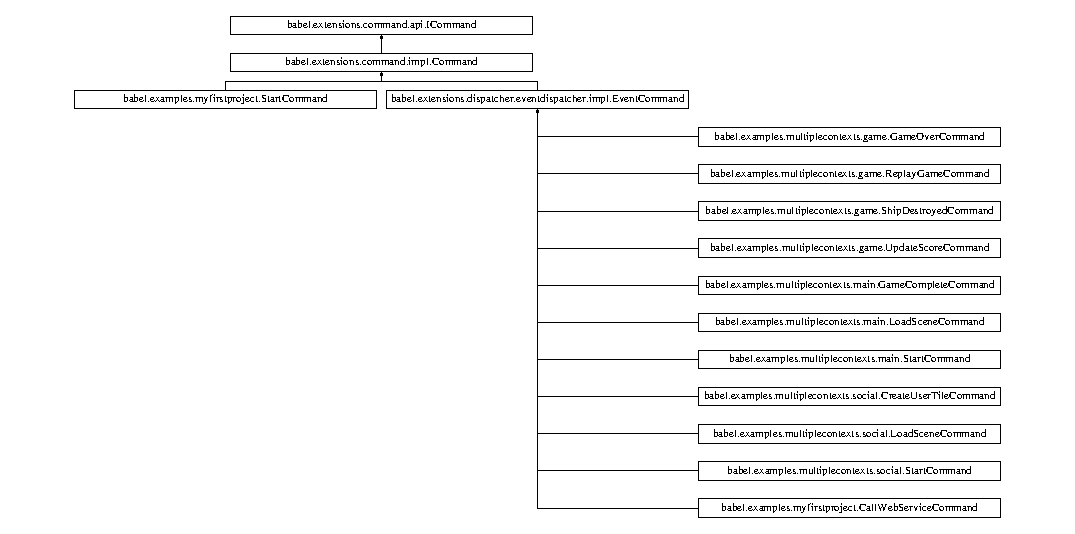
\includegraphics[height=6.735395cm]{interfacebabel_1_1extensions_1_1command_1_1api_1_1_i_command}
\end{center}
\end{figure}
\subsection*{Public Member Functions}
\begin{DoxyCompactItemize}
\item 
\hypertarget{interfacebabel_1_1extensions_1_1command_1_1api_1_1_i_command_afbf19835843cdc4c5c6fea7d2938fa87}{void {\bfseries Execute} ()}\label{interfacebabel_1_1extensions_1_1command_1_1api_1_1_i_command_afbf19835843cdc4c5c6fea7d2938fa87}

\item 
\hypertarget{interfacebabel_1_1extensions_1_1command_1_1api_1_1_i_command_a345704150125e550b485a6025680f7a8}{void {\bfseries Retain} ()}\label{interfacebabel_1_1extensions_1_1command_1_1api_1_1_i_command_a345704150125e550b485a6025680f7a8}

\item 
\hypertarget{interfacebabel_1_1extensions_1_1command_1_1api_1_1_i_command_a67a5dff04956985235b9fe4921288e78}{void {\bfseries Release} ()}\label{interfacebabel_1_1extensions_1_1command_1_1api_1_1_i_command_a67a5dff04956985235b9fe4921288e78}

\item 
\hypertarget{interfacebabel_1_1extensions_1_1command_1_1api_1_1_i_command_a156dbd2fd206e25a06fdb4a5a363867f}{void {\bfseries Dispose} ()}\label{interfacebabel_1_1extensions_1_1command_1_1api_1_1_i_command_a156dbd2fd206e25a06fdb4a5a363867f}

\end{DoxyCompactItemize}
\subsection*{Properties}
\begin{DoxyCompactItemize}
\item 
\hypertarget{interfacebabel_1_1extensions_1_1command_1_1api_1_1_i_command_a2ff6a94dcc8af6d3b35b7731041ae9e4}{bool {\bfseries retain}\hspace{0.3cm}{\ttfamily  \mbox{[}get\mbox{]}}}\label{interfacebabel_1_1extensions_1_1command_1_1api_1_1_i_command_a2ff6a94dcc8af6d3b35b7731041ae9e4}

\item 
\hypertarget{interfacebabel_1_1extensions_1_1command_1_1api_1_1_i_command_a3ac3a3f989ebc5243b8f14fb387dff36}{object {\bfseries data}\hspace{0.3cm}{\ttfamily  \mbox{[}get, set\mbox{]}}}\label{interfacebabel_1_1extensions_1_1command_1_1api_1_1_i_command_a3ac3a3f989ebc5243b8f14fb387dff36}

\end{DoxyCompactItemize}


The documentation for this interface was generated from the following file\-:\begin{DoxyCompactItemize}
\item 
Assets/scripts/babel/extensions/command/api/I\-Command.\-cs\end{DoxyCompactItemize}

\hypertarget{interfacebabel_1_1extensions_1_1command_1_1api_1_1_i_command_binder}{\section{babel.\-extensions.\-command.\-api.\-I\-Command\-Binder Interface Reference}
\label{interfacebabel_1_1extensions_1_1command_1_1api_1_1_i_command_binder}\index{babel.\-extensions.\-command.\-api.\-I\-Command\-Binder@{babel.\-extensions.\-command.\-api.\-I\-Command\-Binder}}
}
Inheritance diagram for babel.\-extensions.\-command.\-api.\-I\-Command\-Binder\-:\begin{figure}[H]
\begin{center}
\leavevmode
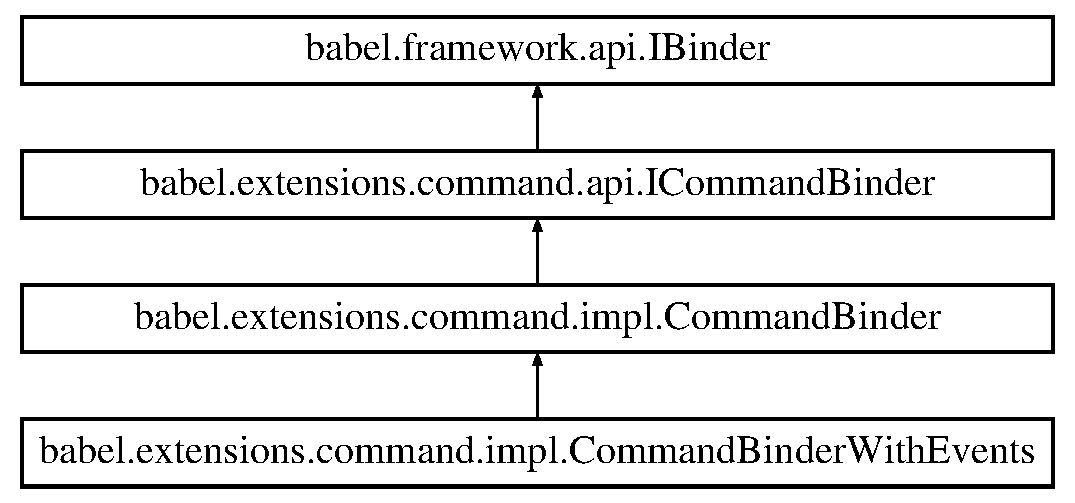
\includegraphics[height=4.000000cm]{interfacebabel_1_1extensions_1_1command_1_1api_1_1_i_command_binder}
\end{center}
\end{figure}
\subsection*{Public Member Functions}
\begin{DoxyCompactItemize}
\item 
void \hyperlink{interfacebabel_1_1extensions_1_1command_1_1api_1_1_i_command_binder_a50e05144d88aa86e46b8d78125667e43}{React\-To} (object trigger)
\begin{DoxyCompactList}\small\item\em Instantiate and execute one or more Commands based on the input. \end{DoxyCompactList}\item 
\hypertarget{interfacebabel_1_1extensions_1_1command_1_1api_1_1_i_command_binder_a7062e414641978e785490334d8b2414b}{void {\bfseries React\-To} (object trigger, object data)}\label{interfacebabel_1_1extensions_1_1command_1_1api_1_1_i_command_binder_a7062e414641978e785490334d8b2414b}

\item 
void \hyperlink{interfacebabel_1_1extensions_1_1command_1_1api_1_1_i_command_binder_a03df21f7c6b2c9628dc00afc34d08a2e}{Release\-Command} (\hyperlink{interfacebabel_1_1extensions_1_1command_1_1api_1_1_i_command}{I\-Command} command)
\begin{DoxyCompactList}\small\item\em Release a previously retained Command. \end{DoxyCompactList}\item 
\hypertarget{interfacebabel_1_1extensions_1_1command_1_1api_1_1_i_command_binder_a5b21a6bf1e355ce44134d4c421901190}{new \hyperlink{interfacebabel_1_1extensions_1_1command_1_1api_1_1_i_command_binding}{I\-Command\-Binding} {\bfseries Bind$<$ T $>$} ()}\label{interfacebabel_1_1extensions_1_1command_1_1api_1_1_i_command_binder_a5b21a6bf1e355ce44134d4c421901190}

\item 
\hypertarget{interfacebabel_1_1extensions_1_1command_1_1api_1_1_i_command_binder_a47f81e31c16288d88c978892bca6c15a}{new \hyperlink{interfacebabel_1_1extensions_1_1command_1_1api_1_1_i_command_binding}{I\-Command\-Binding} {\bfseries Bind} (object value)}\label{interfacebabel_1_1extensions_1_1command_1_1api_1_1_i_command_binder_a47f81e31c16288d88c978892bca6c15a}

\end{DoxyCompactItemize}


\subsection{Member Function Documentation}
\hypertarget{interfacebabel_1_1extensions_1_1command_1_1api_1_1_i_command_binder_a50e05144d88aa86e46b8d78125667e43}{\index{babel\-::extensions\-::command\-::api\-::\-I\-Command\-Binder@{babel\-::extensions\-::command\-::api\-::\-I\-Command\-Binder}!React\-To@{React\-To}}
\index{React\-To@{React\-To}!babel::extensions::command::api::ICommandBinder@{babel\-::extensions\-::command\-::api\-::\-I\-Command\-Binder}}
\subsubsection[{React\-To}]{\setlength{\rightskip}{0pt plus 5cm}void babel.\-extensions.\-command.\-api.\-I\-Command\-Binder.\-React\-To (
\begin{DoxyParamCaption}
\item[{object}]{trigger}
\end{DoxyParamCaption}
)}}\label{interfacebabel_1_1extensions_1_1command_1_1api_1_1_i_command_binder_a50e05144d88aa86e46b8d78125667e43}


Instantiate and execute one or more Commands based on the input. 


\begin{DoxyParams}{Parameters}
{\em trigger} & The key that unlocks the Command(s) \\
\hline
\end{DoxyParams}


Implemented in \hyperlink{classbabel_1_1extensions_1_1command_1_1impl_1_1_command_binder_a9d286dbf28eb4b1ebf7e2c45b8a74d21}{babel.\-extensions.\-command.\-impl.\-Command\-Binder}.

\hypertarget{interfacebabel_1_1extensions_1_1command_1_1api_1_1_i_command_binder_a03df21f7c6b2c9628dc00afc34d08a2e}{\index{babel\-::extensions\-::command\-::api\-::\-I\-Command\-Binder@{babel\-::extensions\-::command\-::api\-::\-I\-Command\-Binder}!Release\-Command@{Release\-Command}}
\index{Release\-Command@{Release\-Command}!babel::extensions::command::api::ICommandBinder@{babel\-::extensions\-::command\-::api\-::\-I\-Command\-Binder}}
\subsubsection[{Release\-Command}]{\setlength{\rightskip}{0pt plus 5cm}void babel.\-extensions.\-command.\-api.\-I\-Command\-Binder.\-Release\-Command (
\begin{DoxyParamCaption}
\item[{{\bf I\-Command}}]{command}
\end{DoxyParamCaption}
)}}\label{interfacebabel_1_1extensions_1_1command_1_1api_1_1_i_command_binder_a03df21f7c6b2c9628dc00afc34d08a2e}


Release a previously retained Command. 

By default, a Command is garbage collected at the end of its Execute method. But the Command can be retained for asynchronous calls.


\begin{DoxyParams}{Parameters}
{\em The} & Command to release \\
\hline
\end{DoxyParams}


Implemented in \hyperlink{classbabel_1_1extensions_1_1command_1_1impl_1_1_command_binder_a5f254fbeda04e19eabdd104458210087}{babel.\-extensions.\-command.\-impl.\-Command\-Binder}.



The documentation for this interface was generated from the following file\-:\begin{DoxyCompactItemize}
\item 
Assets/scripts/babel/extensions/command/api/I\-Command\-Binder.\-cs\end{DoxyCompactItemize}

\hypertarget{interfacebabel_1_1extensions_1_1command_1_1api_1_1_i_command_binding}{\section{babel.\-extensions.\-command.\-api.\-I\-Command\-Binding Interface Reference}
\label{interfacebabel_1_1extensions_1_1command_1_1api_1_1_i_command_binding}\index{babel.\-extensions.\-command.\-api.\-I\-Command\-Binding@{babel.\-extensions.\-command.\-api.\-I\-Command\-Binding}}
}
Inheritance diagram for babel.\-extensions.\-command.\-api.\-I\-Command\-Binding\-:\begin{figure}[H]
\begin{center}
\leavevmode
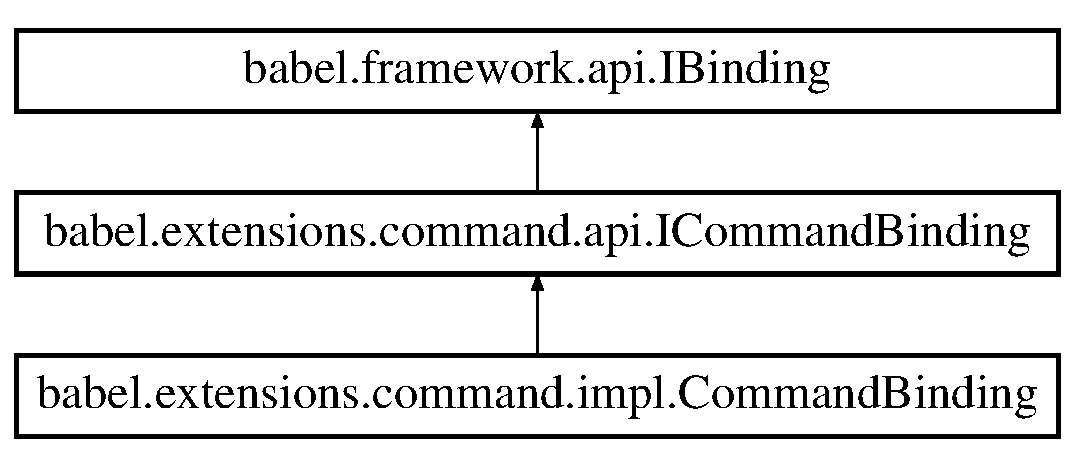
\includegraphics[height=3.000000cm]{interfacebabel_1_1extensions_1_1command_1_1api_1_1_i_command_binding}
\end{center}
\end{figure}
\subsection*{Public Member Functions}
\begin{DoxyCompactItemize}
\item 
\hypertarget{interfacebabel_1_1extensions_1_1command_1_1api_1_1_i_command_binding_a02bcc807f13fd607de629bddeae534b2}{\hyperlink{interfacebabel_1_1extensions_1_1command_1_1api_1_1_i_command_binding}{I\-Command\-Binding} {\bfseries Once} ()}\label{interfacebabel_1_1extensions_1_1command_1_1api_1_1_i_command_binding_a02bcc807f13fd607de629bddeae534b2}

\item 
\hypertarget{interfacebabel_1_1extensions_1_1command_1_1api_1_1_i_command_binding_a4c011da9863b3bfdd985be687c683ed1}{new \hyperlink{interfacebabel_1_1extensions_1_1command_1_1api_1_1_i_command_binding}{I\-Command\-Binding} \hyperlink{interfacebabel_1_1extensions_1_1command_1_1api_1_1_i_command_binding_a4c011da9863b3bfdd985be687c683ed1}{Key$<$ T $>$} ()}\label{interfacebabel_1_1extensions_1_1command_1_1api_1_1_i_command_binding_a4c011da9863b3bfdd985be687c683ed1}

\begin{DoxyCompactList}\small\item\em Below this point is facade for I\-Binding. \end{DoxyCompactList}\item 
\hypertarget{interfacebabel_1_1extensions_1_1command_1_1api_1_1_i_command_binding_a4080aa1ac6b3a76d2975d0082163c262}{new \hyperlink{interfacebabel_1_1extensions_1_1command_1_1api_1_1_i_command_binding}{I\-Command\-Binding} {\bfseries Key} (object key)}\label{interfacebabel_1_1extensions_1_1command_1_1api_1_1_i_command_binding_a4080aa1ac6b3a76d2975d0082163c262}

\item 
\hypertarget{interfacebabel_1_1extensions_1_1command_1_1api_1_1_i_command_binding_ac8b152f51072be19252c7181f4e692c7}{new \hyperlink{interfacebabel_1_1extensions_1_1command_1_1api_1_1_i_command_binding}{I\-Command\-Binding} {\bfseries To$<$ T $>$} ()}\label{interfacebabel_1_1extensions_1_1command_1_1api_1_1_i_command_binding_ac8b152f51072be19252c7181f4e692c7}

\item 
\hypertarget{interfacebabel_1_1extensions_1_1command_1_1api_1_1_i_command_binding_a0ecb0cc33e3ace6a9622808b02816ae5}{new \hyperlink{interfacebabel_1_1extensions_1_1command_1_1api_1_1_i_command_binding}{I\-Command\-Binding} {\bfseries To} (object o)}\label{interfacebabel_1_1extensions_1_1command_1_1api_1_1_i_command_binding_a0ecb0cc33e3ace6a9622808b02816ae5}

\item 
\hypertarget{interfacebabel_1_1extensions_1_1command_1_1api_1_1_i_command_binding_a15415a340496a86a18311dd90fdefbbc}{new \hyperlink{interfacebabel_1_1extensions_1_1command_1_1api_1_1_i_command_binding}{I\-Command\-Binding} {\bfseries To\-Name$<$ T $>$} ()}\label{interfacebabel_1_1extensions_1_1command_1_1api_1_1_i_command_binding_a15415a340496a86a18311dd90fdefbbc}

\item 
\hypertarget{interfacebabel_1_1extensions_1_1command_1_1api_1_1_i_command_binding_aa02a5921bf65ed12f82d8f7ba55e8cc6}{new \hyperlink{interfacebabel_1_1extensions_1_1command_1_1api_1_1_i_command_binding}{I\-Command\-Binding} {\bfseries To\-Name} (object o)}\label{interfacebabel_1_1extensions_1_1command_1_1api_1_1_i_command_binding_aa02a5921bf65ed12f82d8f7ba55e8cc6}

\item 
\hypertarget{interfacebabel_1_1extensions_1_1command_1_1api_1_1_i_command_binding_a30fd56f00f01343c6c93003b9d10563f}{new \hyperlink{interfacebabel_1_1extensions_1_1command_1_1api_1_1_i_command_binding}{I\-Command\-Binding} {\bfseries Named$<$ T $>$} ()}\label{interfacebabel_1_1extensions_1_1command_1_1api_1_1_i_command_binding_a30fd56f00f01343c6c93003b9d10563f}

\item 
\hypertarget{interfacebabel_1_1extensions_1_1command_1_1api_1_1_i_command_binding_ac7d322da8ff7dcd3705d91ecd0f37665}{new \hyperlink{interfacebabel_1_1extensions_1_1command_1_1api_1_1_i_command_binding}{I\-Command\-Binding} {\bfseries Named} (object o)}\label{interfacebabel_1_1extensions_1_1command_1_1api_1_1_i_command_binding_ac7d322da8ff7dcd3705d91ecd0f37665}

\end{DoxyCompactItemize}
\subsection*{Properties}
\begin{DoxyCompactItemize}
\item 
\hypertarget{interfacebabel_1_1extensions_1_1command_1_1api_1_1_i_command_binding_aa51a5682b647d02f867fda10f3315c54}{bool {\bfseries is\-One\-Off}\hspace{0.3cm}{\ttfamily  \mbox{[}get, set\mbox{]}}}\label{interfacebabel_1_1extensions_1_1command_1_1api_1_1_i_command_binding_aa51a5682b647d02f867fda10f3315c54}

\end{DoxyCompactItemize}


The documentation for this interface was generated from the following file\-:\begin{DoxyCompactItemize}
\item 
Assets/scripts/babel/extensions/command/api/I\-Command\-Binding.\-cs\end{DoxyCompactItemize}

\hypertarget{interfacebabel_1_1extensions_1_1context_1_1api_1_1_i_context}{\section{babel.\-extensions.\-context.\-api.\-I\-Context Interface Reference}
\label{interfacebabel_1_1extensions_1_1context_1_1api_1_1_i_context}\index{babel.\-extensions.\-context.\-api.\-I\-Context@{babel.\-extensions.\-context.\-api.\-I\-Context}}
}
Inheritance diagram for babel.\-extensions.\-context.\-api.\-I\-Context\-:\begin{figure}[H]
\begin{center}
\leavevmode
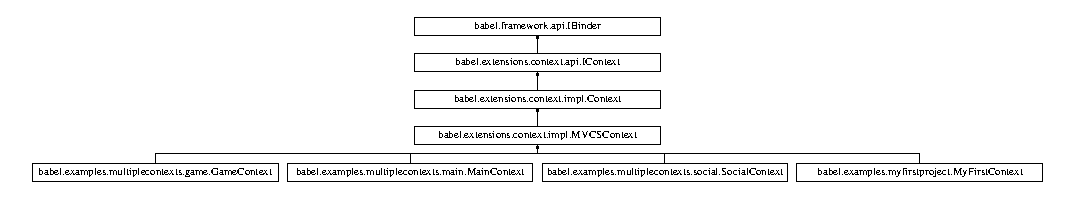
\includegraphics[height=2.208202cm]{interfacebabel_1_1extensions_1_1context_1_1api_1_1_i_context}
\end{center}
\end{figure}
\subsection*{Public Member Functions}
\begin{DoxyCompactItemize}
\item 
\hypertarget{interfacebabel_1_1extensions_1_1context_1_1api_1_1_i_context_a81cd829cd3944621bcf8cb586caeecd0}{\hyperlink{interfacebabel_1_1extensions_1_1context_1_1api_1_1_i_context}{I\-Context} {\bfseries Start} ()}\label{interfacebabel_1_1extensions_1_1context_1_1api_1_1_i_context_a81cd829cd3944621bcf8cb586caeecd0}

\item 
\hypertarget{interfacebabel_1_1extensions_1_1context_1_1api_1_1_i_context_af4d39ee0ad504a69bc7f6b9145fb1a66}{object {\bfseries Get\-Component$<$ T $>$} ()}\label{interfacebabel_1_1extensions_1_1context_1_1api_1_1_i_context_af4d39ee0ad504a69bc7f6b9145fb1a66}

\item 
\hypertarget{interfacebabel_1_1extensions_1_1context_1_1api_1_1_i_context_a507b940e5f9236218c816cdd2d540ab5}{object {\bfseries Get\-Component$<$ T $>$} (object name)}\label{interfacebabel_1_1extensions_1_1context_1_1api_1_1_i_context_a507b940e5f9236218c816cdd2d540ab5}

\item 
\hypertarget{interfacebabel_1_1extensions_1_1context_1_1api_1_1_i_context_afda73a4a51b2569aeaefeb3ce44f095b}{\hyperlink{interfacebabel_1_1extensions_1_1context_1_1api_1_1_i_context}{I\-Context} {\bfseries Add\-Context} (\hyperlink{interfacebabel_1_1extensions_1_1context_1_1api_1_1_i_context}{I\-Context} context)}\label{interfacebabel_1_1extensions_1_1context_1_1api_1_1_i_context_afda73a4a51b2569aeaefeb3ce44f095b}

\item 
\hypertarget{interfacebabel_1_1extensions_1_1context_1_1api_1_1_i_context_ad281420ff6ccbb9279cb7c6fea57a339}{\hyperlink{interfacebabel_1_1extensions_1_1context_1_1api_1_1_i_context}{I\-Context} {\bfseries Remove\-Context} (\hyperlink{interfacebabel_1_1extensions_1_1context_1_1api_1_1_i_context}{I\-Context} context)}\label{interfacebabel_1_1extensions_1_1context_1_1api_1_1_i_context_ad281420ff6ccbb9279cb7c6fea57a339}

\item 
\hypertarget{interfacebabel_1_1extensions_1_1context_1_1api_1_1_i_context_af8eb0c716a95e9d41f29ffe33c69cd73}{void {\bfseries Add\-View} (object view)}\label{interfacebabel_1_1extensions_1_1context_1_1api_1_1_i_context_af8eb0c716a95e9d41f29ffe33c69cd73}

\item 
\hypertarget{interfacebabel_1_1extensions_1_1context_1_1api_1_1_i_context_a75f3c7d1e15261e3b2028660ac26ecb4}{void {\bfseries Remove\-View} (object view)}\label{interfacebabel_1_1extensions_1_1context_1_1api_1_1_i_context_a75f3c7d1e15261e3b2028660ac26ecb4}

\end{DoxyCompactItemize}
\subsection*{Properties}
\begin{DoxyCompactItemize}
\item 
\hypertarget{interfacebabel_1_1extensions_1_1context_1_1api_1_1_i_context_a1e4e810b390bcf65445821a05050680a}{\hyperlink{interfacebabel_1_1extensions_1_1dispatcher_1_1api_1_1_i_dispatcher}{I\-Dispatcher} {\bfseries cross\-Context\-Dispatcher}\hspace{0.3cm}{\ttfamily  \mbox{[}get, set\mbox{]}}}\label{interfacebabel_1_1extensions_1_1context_1_1api_1_1_i_context_a1e4e810b390bcf65445821a05050680a}

\end{DoxyCompactItemize}


The documentation for this interface was generated from the following file\-:\begin{DoxyCompactItemize}
\item 
Assets/scripts/babel/extensions/context/api/I\-Context.\-cs\end{DoxyCompactItemize}

\hypertarget{interfacebabel_1_1extensions_1_1context_1_1api_1_1_i_context_view}{\section{babel.\-extensions.\-context.\-api.\-I\-Context\-View Interface Reference}
\label{interfacebabel_1_1extensions_1_1context_1_1api_1_1_i_context_view}\index{babel.\-extensions.\-context.\-api.\-I\-Context\-View@{babel.\-extensions.\-context.\-api.\-I\-Context\-View}}
}
Inheritance diagram for babel.\-extensions.\-context.\-api.\-I\-Context\-View\-:\begin{figure}[H]
\begin{center}
\leavevmode
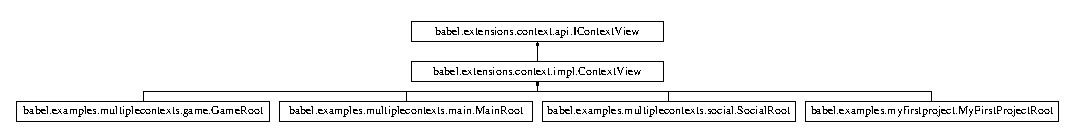
\includegraphics[height=1.400000cm]{interfacebabel_1_1extensions_1_1context_1_1api_1_1_i_context_view}
\end{center}
\end{figure}
\subsection*{Properties}
\begin{DoxyCompactItemize}
\item 
\hypertarget{interfacebabel_1_1extensions_1_1context_1_1api_1_1_i_context_view_a6145e964d20dacbccbd395201c89ffa5}{\hyperlink{interfacebabel_1_1extensions_1_1context_1_1api_1_1_i_context}{I\-Context} {\bfseries context}\hspace{0.3cm}{\ttfamily  \mbox{[}get, set\mbox{]}}}\label{interfacebabel_1_1extensions_1_1context_1_1api_1_1_i_context_view_a6145e964d20dacbccbd395201c89ffa5}

\end{DoxyCompactItemize}


The documentation for this interface was generated from the following file\-:\begin{DoxyCompactItemize}
\item 
Assets/scripts/babel/extensions/context/api/I\-Context\-View.\-cs\end{DoxyCompactItemize}

\hypertarget{interfacebabel_1_1extensions_1_1dispatcher_1_1api_1_1_i_dispatcher}{\section{babel.\-extensions.\-dispatcher.\-api.\-I\-Dispatcher Interface Reference}
\label{interfacebabel_1_1extensions_1_1dispatcher_1_1api_1_1_i_dispatcher}\index{babel.\-extensions.\-dispatcher.\-api.\-I\-Dispatcher@{babel.\-extensions.\-dispatcher.\-api.\-I\-Dispatcher}}
}
Inheritance diagram for babel.\-extensions.\-dispatcher.\-api.\-I\-Dispatcher\-:\begin{figure}[H]
\begin{center}
\leavevmode
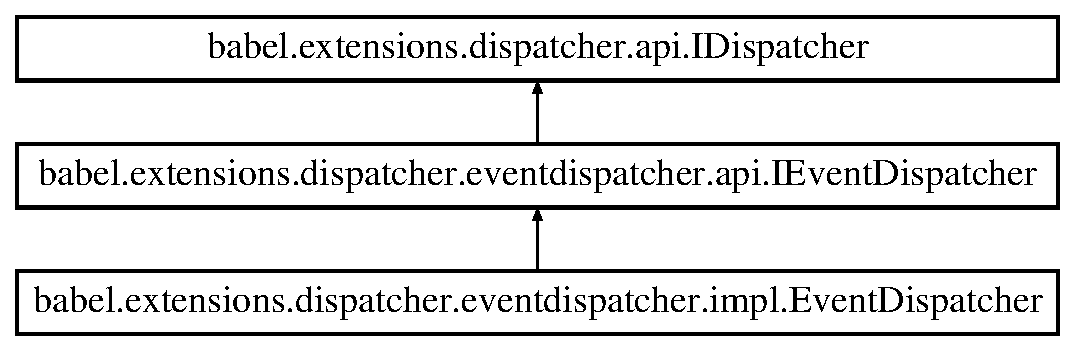
\includegraphics[height=3.000000cm]{interfacebabel_1_1extensions_1_1dispatcher_1_1api_1_1_i_dispatcher}
\end{center}
\end{figure}
\subsection*{Public Member Functions}
\begin{DoxyCompactItemize}
\item 
\hypertarget{interfacebabel_1_1extensions_1_1dispatcher_1_1api_1_1_i_dispatcher_aef13e28dbeb27ac9421d89d5297a1aef}{void {\bfseries Dispatch} (object event\-Type)}\label{interfacebabel_1_1extensions_1_1dispatcher_1_1api_1_1_i_dispatcher_aef13e28dbeb27ac9421d89d5297a1aef}

\item 
\hypertarget{interfacebabel_1_1extensions_1_1dispatcher_1_1api_1_1_i_dispatcher_aa4a78e9cdc5e87440481ba405e0af521}{void {\bfseries Dispatch} (object event\-Type, object data)}\label{interfacebabel_1_1extensions_1_1dispatcher_1_1api_1_1_i_dispatcher_aa4a78e9cdc5e87440481ba405e0af521}

\end{DoxyCompactItemize}


The documentation for this interface was generated from the following file\-:\begin{DoxyCompactItemize}
\item 
Assets/scripts/babel/extensions/dispatcher/api/I\-Dispatcher.\-cs\end{DoxyCompactItemize}

\hypertarget{interfacebabel_1_1extensions_1_1dispatcher_1_1eventdispatcher_1_1api_1_1_i_event_binding}{\section{babel.\-extensions.\-dispatcher.\-eventdispatcher.\-api.\-I\-Event\-Binding Interface Reference}
\label{interfacebabel_1_1extensions_1_1dispatcher_1_1eventdispatcher_1_1api_1_1_i_event_binding}\index{babel.\-extensions.\-dispatcher.\-eventdispatcher.\-api.\-I\-Event\-Binding@{babel.\-extensions.\-dispatcher.\-eventdispatcher.\-api.\-I\-Event\-Binding}}
}
Inheritance diagram for babel.\-extensions.\-dispatcher.\-eventdispatcher.\-api.\-I\-Event\-Binding\-:\begin{figure}[H]
\begin{center}
\leavevmode
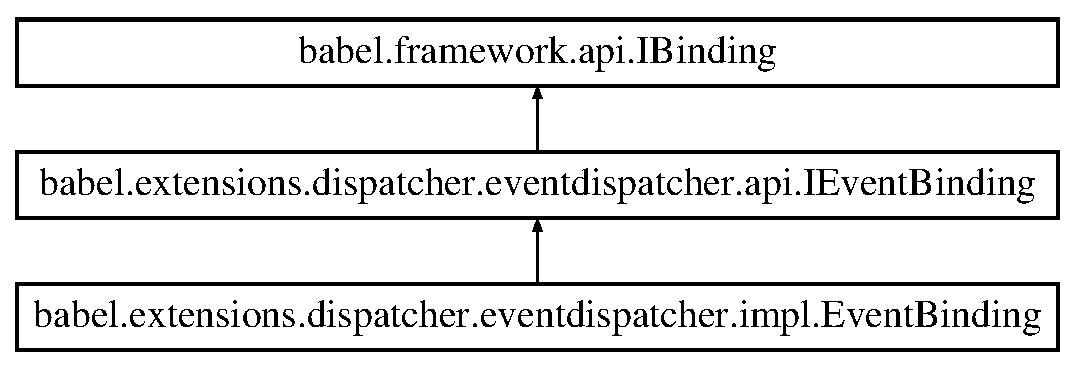
\includegraphics[height=3.000000cm]{interfacebabel_1_1extensions_1_1dispatcher_1_1eventdispatcher_1_1api_1_1_i_event_binding}
\end{center}
\end{figure}
\subsection*{Public Member Functions}
\begin{DoxyCompactItemize}
\item 
\hypertarget{interfacebabel_1_1extensions_1_1dispatcher_1_1eventdispatcher_1_1api_1_1_i_event_binding_ab087de794f1a13a33e5c3f3f634e0c4c}{Event\-Callback\-Type {\bfseries type\-For\-Callback} (Event\-Callback callback)}\label{interfacebabel_1_1extensions_1_1dispatcher_1_1eventdispatcher_1_1api_1_1_i_event_binding_ab087de794f1a13a33e5c3f3f634e0c4c}

\item 
\hypertarget{interfacebabel_1_1extensions_1_1dispatcher_1_1eventdispatcher_1_1api_1_1_i_event_binding_a0ce7fcf1e89a0d337cd944c4ff851f08}{Event\-Callback\-Type {\bfseries type\-For\-Callback} (Empty\-Callback callback)}\label{interfacebabel_1_1extensions_1_1dispatcher_1_1eventdispatcher_1_1api_1_1_i_event_binding_a0ce7fcf1e89a0d337cd944c4ff851f08}

\item 
\hypertarget{interfacebabel_1_1extensions_1_1dispatcher_1_1eventdispatcher_1_1api_1_1_i_event_binding_afaa0ecbcf35d2a9be40fb1228d00ee5a}{new \hyperlink{interfacebabel_1_1extensions_1_1dispatcher_1_1eventdispatcher_1_1api_1_1_i_event_binding}{I\-Event\-Binding} {\bfseries Key} (object key)}\label{interfacebabel_1_1extensions_1_1dispatcher_1_1eventdispatcher_1_1api_1_1_i_event_binding_afaa0ecbcf35d2a9be40fb1228d00ee5a}

\item 
\hypertarget{interfacebabel_1_1extensions_1_1dispatcher_1_1eventdispatcher_1_1api_1_1_i_event_binding_a559f4d8669986c348959731f92b1e637}{\hyperlink{interfacebabel_1_1extensions_1_1dispatcher_1_1eventdispatcher_1_1api_1_1_i_event_binding}{I\-Event\-Binding} {\bfseries To} (Event\-Callback callback)}\label{interfacebabel_1_1extensions_1_1dispatcher_1_1eventdispatcher_1_1api_1_1_i_event_binding_a559f4d8669986c348959731f92b1e637}

\item 
\hypertarget{interfacebabel_1_1extensions_1_1dispatcher_1_1eventdispatcher_1_1api_1_1_i_event_binding_aed033ce9edb5081eeaab36005207ca4e}{\hyperlink{interfacebabel_1_1extensions_1_1dispatcher_1_1eventdispatcher_1_1api_1_1_i_event_binding}{I\-Event\-Binding} {\bfseries To} (Empty\-Callback callback)}\label{interfacebabel_1_1extensions_1_1dispatcher_1_1eventdispatcher_1_1api_1_1_i_event_binding_aed033ce9edb5081eeaab36005207ca4e}

\end{DoxyCompactItemize}
\subsection*{Additional Inherited Members}


The documentation for this interface was generated from the following file\-:\begin{DoxyCompactItemize}
\item 
Assets/scripts/babel/extensions/dispatcher/eventdispatcher/api/I\-Event\-Binding.\-cs\end{DoxyCompactItemize}

\hypertarget{interfacebabel_1_1extensions_1_1dispatcher_1_1eventdispatcher_1_1api_1_1_i_event_dispatcher}{\section{babel.\-extensions.\-dispatcher.\-eventdispatcher.\-api.\-I\-Event\-Dispatcher Interface Reference}
\label{interfacebabel_1_1extensions_1_1dispatcher_1_1eventdispatcher_1_1api_1_1_i_event_dispatcher}\index{babel.\-extensions.\-dispatcher.\-eventdispatcher.\-api.\-I\-Event\-Dispatcher@{babel.\-extensions.\-dispatcher.\-eventdispatcher.\-api.\-I\-Event\-Dispatcher}}
}
Inheritance diagram for babel.\-extensions.\-dispatcher.\-eventdispatcher.\-api.\-I\-Event\-Dispatcher\-:\begin{figure}[H]
\begin{center}
\leavevmode
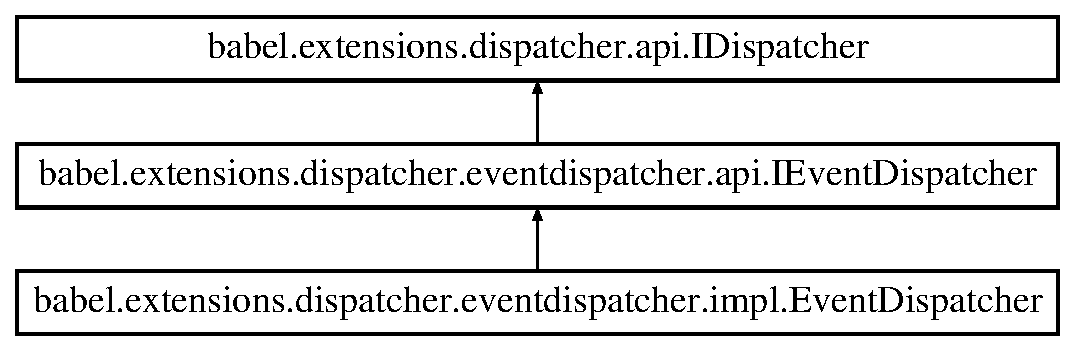
\includegraphics[height=3.000000cm]{interfacebabel_1_1extensions_1_1dispatcher_1_1eventdispatcher_1_1api_1_1_i_event_dispatcher}
\end{center}
\end{figure}
\subsection*{Public Member Functions}
\begin{DoxyCompactItemize}
\item 
\hypertarget{interfacebabel_1_1extensions_1_1dispatcher_1_1eventdispatcher_1_1api_1_1_i_event_dispatcher_a934a75f6ea05960ae158a2fda0c7dda7}{\hyperlink{interfacebabel_1_1extensions_1_1dispatcher_1_1eventdispatcher_1_1api_1_1_i_event_binding}{I\-Event\-Binding} {\bfseries Bind} (object key)}\label{interfacebabel_1_1extensions_1_1dispatcher_1_1eventdispatcher_1_1api_1_1_i_event_dispatcher_a934a75f6ea05960ae158a2fda0c7dda7}

\item 
\hypertarget{interfacebabel_1_1extensions_1_1dispatcher_1_1eventdispatcher_1_1api_1_1_i_event_dispatcher_a8dd44e68104270f09c7455d8ab39c271}{void {\bfseries add\-Listener} (object evt, Event\-Callback callback)}\label{interfacebabel_1_1extensions_1_1dispatcher_1_1eventdispatcher_1_1api_1_1_i_event_dispatcher_a8dd44e68104270f09c7455d8ab39c271}

\item 
\hypertarget{interfacebabel_1_1extensions_1_1dispatcher_1_1eventdispatcher_1_1api_1_1_i_event_dispatcher_a04e9eebfe3b841d08c3c263c7741a77c}{void {\bfseries add\-Listener} (object evt, Empty\-Callback callback)}\label{interfacebabel_1_1extensions_1_1dispatcher_1_1eventdispatcher_1_1api_1_1_i_event_dispatcher_a04e9eebfe3b841d08c3c263c7741a77c}

\item 
\hypertarget{interfacebabel_1_1extensions_1_1dispatcher_1_1eventdispatcher_1_1api_1_1_i_event_dispatcher_a3dc280e1a7338838e66055d164959e3e}{void {\bfseries remove\-Listener} (object evt, Event\-Callback callback)}\label{interfacebabel_1_1extensions_1_1dispatcher_1_1eventdispatcher_1_1api_1_1_i_event_dispatcher_a3dc280e1a7338838e66055d164959e3e}

\item 
\hypertarget{interfacebabel_1_1extensions_1_1dispatcher_1_1eventdispatcher_1_1api_1_1_i_event_dispatcher_ae6576ff4221aee409a2f6d1d01eaaf31}{void {\bfseries remove\-Listener} (object evt, Empty\-Callback callback)}\label{interfacebabel_1_1extensions_1_1dispatcher_1_1eventdispatcher_1_1api_1_1_i_event_dispatcher_ae6576ff4221aee409a2f6d1d01eaaf31}

\item 
\hypertarget{interfacebabel_1_1extensions_1_1dispatcher_1_1eventdispatcher_1_1api_1_1_i_event_dispatcher_a5648e37cc6b71be8746c215f7f75b8d3}{bool {\bfseries has\-Listener} (object evt, Event\-Callback callback)}\label{interfacebabel_1_1extensions_1_1dispatcher_1_1eventdispatcher_1_1api_1_1_i_event_dispatcher_a5648e37cc6b71be8746c215f7f75b8d3}

\item 
\hypertarget{interfacebabel_1_1extensions_1_1dispatcher_1_1eventdispatcher_1_1api_1_1_i_event_dispatcher_ac0a3baded9a7501e426549677a0b415a}{bool {\bfseries has\-Listener} (object evt, Empty\-Callback callback)}\label{interfacebabel_1_1extensions_1_1dispatcher_1_1eventdispatcher_1_1api_1_1_i_event_dispatcher_ac0a3baded9a7501e426549677a0b415a}

\item 
\hypertarget{interfacebabel_1_1extensions_1_1dispatcher_1_1eventdispatcher_1_1api_1_1_i_event_dispatcher_a5d2befa659d1aca834821ce0988dc2c2}{void {\bfseries update\-Listener} (bool to\-Add, object evt, Event\-Callback callback)}\label{interfacebabel_1_1extensions_1_1dispatcher_1_1eventdispatcher_1_1api_1_1_i_event_dispatcher_a5d2befa659d1aca834821ce0988dc2c2}

\item 
\hypertarget{interfacebabel_1_1extensions_1_1dispatcher_1_1eventdispatcher_1_1api_1_1_i_event_dispatcher_a43b8e4ea52e4a93cd268c04b17cd792a}{void {\bfseries update\-Listener} (bool to\-Add, object evt, Empty\-Callback callback)}\label{interfacebabel_1_1extensions_1_1dispatcher_1_1eventdispatcher_1_1api_1_1_i_event_dispatcher_a43b8e4ea52e4a93cd268c04b17cd792a}

\end{DoxyCompactItemize}


The documentation for this interface was generated from the following file\-:\begin{DoxyCompactItemize}
\item 
Assets/scripts/babel/extensions/dispatcher/eventdispatcher/api/I\-Event\-Dispatcher.\-cs\end{DoxyCompactItemize}

\hypertarget{interfacebabel_1_1examples_1_1myfirstproject_1_1_i_example_model}{\section{babel.\-examples.\-myfirstproject.\-I\-Example\-Model Interface Reference}
\label{interfacebabel_1_1examples_1_1myfirstproject_1_1_i_example_model}\index{babel.\-examples.\-myfirstproject.\-I\-Example\-Model@{babel.\-examples.\-myfirstproject.\-I\-Example\-Model}}
}
Inheritance diagram for babel.\-examples.\-myfirstproject.\-I\-Example\-Model\-:\begin{figure}[H]
\begin{center}
\leavevmode
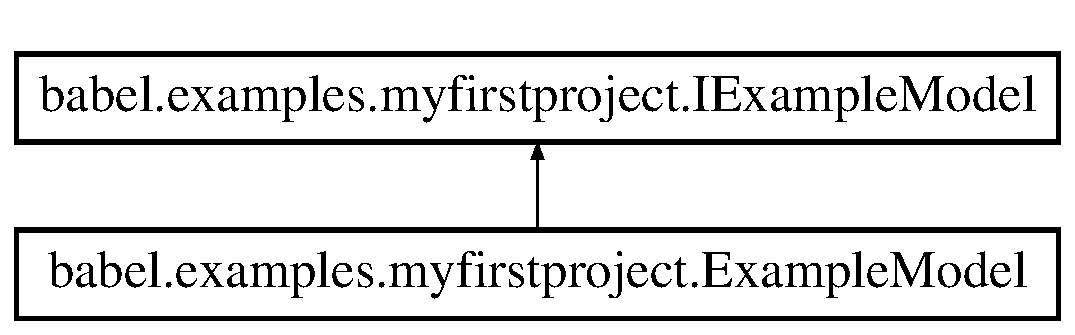
\includegraphics[height=2.000000cm]{interfacebabel_1_1examples_1_1myfirstproject_1_1_i_example_model}
\end{center}
\end{figure}
\subsection*{Properties}
\begin{DoxyCompactItemize}
\item 
\hypertarget{interfacebabel_1_1examples_1_1myfirstproject_1_1_i_example_model_abc1701f082259cd73965fe9e2db7298f}{string {\bfseries data}\hspace{0.3cm}{\ttfamily  \mbox{[}get, set\mbox{]}}}\label{interfacebabel_1_1examples_1_1myfirstproject_1_1_i_example_model_abc1701f082259cd73965fe9e2db7298f}

\end{DoxyCompactItemize}


The documentation for this interface was generated from the following file\-:\begin{DoxyCompactItemize}
\item 
Assets/scripts/babel/examples/myfirstproject/model/I\-Example\-Model.\-cs\end{DoxyCompactItemize}

\hypertarget{interfacebabel_1_1examples_1_1myfirstproject_1_1_i_example_service}{\section{babel.\-examples.\-myfirstproject.\-I\-Example\-Service Interface Reference}
\label{interfacebabel_1_1examples_1_1myfirstproject_1_1_i_example_service}\index{babel.\-examples.\-myfirstproject.\-I\-Example\-Service@{babel.\-examples.\-myfirstproject.\-I\-Example\-Service}}
}
Inheritance diagram for babel.\-examples.\-myfirstproject.\-I\-Example\-Service\-:\begin{figure}[H]
\begin{center}
\leavevmode
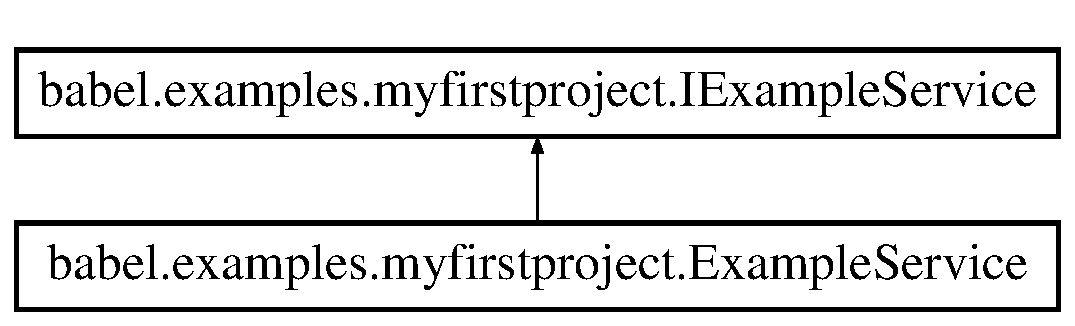
\includegraphics[height=2.000000cm]{interfacebabel_1_1examples_1_1myfirstproject_1_1_i_example_service}
\end{center}
\end{figure}
\subsection*{Public Member Functions}
\begin{DoxyCompactItemize}
\item 
\hypertarget{interfacebabel_1_1examples_1_1myfirstproject_1_1_i_example_service_a0380c5f6a20bcbf018a1fd43381ee077}{void {\bfseries Request} (string url)}\label{interfacebabel_1_1examples_1_1myfirstproject_1_1_i_example_service_a0380c5f6a20bcbf018a1fd43381ee077}

\end{DoxyCompactItemize}
\subsection*{Properties}
\begin{DoxyCompactItemize}
\item 
\hypertarget{interfacebabel_1_1examples_1_1myfirstproject_1_1_i_example_service_ac69f89838133faecbd25046a50a4a465}{\hyperlink{interfacebabel_1_1extensions_1_1dispatcher_1_1eventdispatcher_1_1api_1_1_i_event_dispatcher}{I\-Event\-Dispatcher} {\bfseries dispatcher}\hspace{0.3cm}{\ttfamily  \mbox{[}get, set\mbox{]}}}\label{interfacebabel_1_1examples_1_1myfirstproject_1_1_i_example_service_ac69f89838133faecbd25046a50a4a465}

\end{DoxyCompactItemize}


The documentation for this interface was generated from the following file\-:\begin{DoxyCompactItemize}
\item 
Assets/scripts/babel/examples/myfirstproject/service/I\-Example\-Service.\-cs\end{DoxyCompactItemize}

\hypertarget{interfacebabel_1_1framework_1_1api_1_1_i_factory}{\section{babel.\-framework.\-api.\-I\-Factory Interface Reference}
\label{interfacebabel_1_1framework_1_1api_1_1_i_factory}\index{babel.\-framework.\-api.\-I\-Factory@{babel.\-framework.\-api.\-I\-Factory}}
}
\subsection*{Public Member Functions}
\begin{DoxyCompactItemize}
\item 
\hypertarget{interfacebabel_1_1framework_1_1api_1_1_i_factory_a7f662dbd64b41086da6753c8f8b84fd1}{object {\bfseries Get} (\hyperlink{interfacebabel_1_1framework_1_1api_1_1_i_binding}{I\-Binding} binding)}\label{interfacebabel_1_1framework_1_1api_1_1_i_factory_a7f662dbd64b41086da6753c8f8b84fd1}

\item 
\hypertarget{interfacebabel_1_1framework_1_1api_1_1_i_factory_a29c73d96c1ddb1699e478d5d2004a065}{object {\bfseries Get} (\hyperlink{interfacebabel_1_1framework_1_1api_1_1_i_binding}{I\-Binding} binding, object\mbox{[}$\,$\mbox{]} args)}\label{interfacebabel_1_1framework_1_1api_1_1_i_factory_a29c73d96c1ddb1699e478d5d2004a065}

\end{DoxyCompactItemize}


The documentation for this interface was generated from the following file\-:\begin{DoxyCompactItemize}
\item 
Assets/scripts/babel/framework/api/I\-Factory.\-cs\end{DoxyCompactItemize}

\hypertarget{interfacebabel_1_1examples_1_1multiplecontexts_1_1game_1_1_i_game_timer}{\section{babel.\-examples.\-multiplecontexts.\-game.\-I\-Game\-Timer Interface Reference}
\label{interfacebabel_1_1examples_1_1multiplecontexts_1_1game_1_1_i_game_timer}\index{babel.\-examples.\-multiplecontexts.\-game.\-I\-Game\-Timer@{babel.\-examples.\-multiplecontexts.\-game.\-I\-Game\-Timer}}
}
Inheritance diagram for babel.\-examples.\-multiplecontexts.\-game.\-I\-Game\-Timer\-:\begin{figure}[H]
\begin{center}
\leavevmode
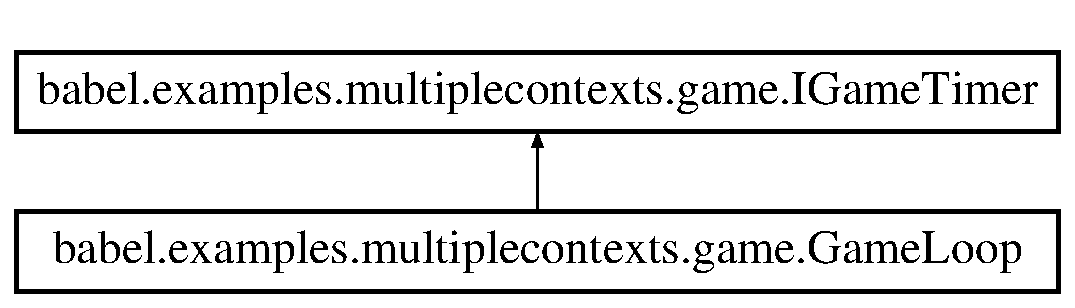
\includegraphics[height=2.000000cm]{interfacebabel_1_1examples_1_1multiplecontexts_1_1game_1_1_i_game_timer}
\end{center}
\end{figure}
\subsection*{Public Member Functions}
\begin{DoxyCompactItemize}
\item 
\hypertarget{interfacebabel_1_1examples_1_1multiplecontexts_1_1game_1_1_i_game_timer_a46f75700d7a966a9e176655780a23ddf}{void {\bfseries Start} ()}\label{interfacebabel_1_1examples_1_1multiplecontexts_1_1game_1_1_i_game_timer_a46f75700d7a966a9e176655780a23ddf}

\item 
\hypertarget{interfacebabel_1_1examples_1_1multiplecontexts_1_1game_1_1_i_game_timer_abcfff36211863edd49819e74fb187ad7}{void {\bfseries Stop} ()}\label{interfacebabel_1_1examples_1_1multiplecontexts_1_1game_1_1_i_game_timer_abcfff36211863edd49819e74fb187ad7}

\end{DoxyCompactItemize}


The documentation for this interface was generated from the following file\-:\begin{DoxyCompactItemize}
\item 
Assets/scripts/babel/examples/multiplecontexts/game/util/I\-Game\-Timer.\-cs\end{DoxyCompactItemize}

\hypertarget{interfacebabel_1_1extensions_1_1injector_1_1api_1_1_i_injection_binder}{\section{babel.\-extensions.\-injector.\-api.\-I\-Injection\-Binder Interface Reference}
\label{interfacebabel_1_1extensions_1_1injector_1_1api_1_1_i_injection_binder}\index{babel.\-extensions.\-injector.\-api.\-I\-Injection\-Binder@{babel.\-extensions.\-injector.\-api.\-I\-Injection\-Binder}}
}
Inheritance diagram for babel.\-extensions.\-injector.\-api.\-I\-Injection\-Binder\-:\begin{figure}[H]
\begin{center}
\leavevmode
\includegraphics[height=2.000000cm]{interfacebabel_1_1extensions_1_1injector_1_1api_1_1_i_injection_binder}
\end{center}
\end{figure}
\subsection*{Public Member Functions}
\begin{DoxyCompactItemize}
\item 
\hypertarget{interfacebabel_1_1extensions_1_1injector_1_1api_1_1_i_injection_binder_ad6ed04286a44d0f663b8059a31930463}{object {\bfseries Get\-Instance} (Type key)}\label{interfacebabel_1_1extensions_1_1injector_1_1api_1_1_i_injection_binder_ad6ed04286a44d0f663b8059a31930463}

\item 
\hypertarget{interfacebabel_1_1extensions_1_1injector_1_1api_1_1_i_injection_binder_a8a41484e318e83ac39c5c9955c5eda2f}{object {\bfseries Get\-Instance} (Type key, object name)}\label{interfacebabel_1_1extensions_1_1injector_1_1api_1_1_i_injection_binder_a8a41484e318e83ac39c5c9955c5eda2f}

\item 
\hypertarget{interfacebabel_1_1extensions_1_1injector_1_1api_1_1_i_injection_binder_a4a66d96e9b32dc1ffaa970ab0d794867}{object {\bfseries Get\-Instance$<$ T $>$} ()}\label{interfacebabel_1_1extensions_1_1injector_1_1api_1_1_i_injection_binder_a4a66d96e9b32dc1ffaa970ab0d794867}

\item 
\hypertarget{interfacebabel_1_1extensions_1_1injector_1_1api_1_1_i_injection_binder_a995f605235373c576b351f00e325dc77}{object {\bfseries Get\-Instance$<$ T $>$} (object name)}\label{interfacebabel_1_1extensions_1_1injector_1_1api_1_1_i_injection_binder_a995f605235373c576b351f00e325dc77}

\item 
\hypertarget{interfacebabel_1_1extensions_1_1injector_1_1api_1_1_i_injection_binder_a49a5cb8d9da05ec35fbc73a8fc1a49a7}{\hyperlink{interfacebabel_1_1extensions_1_1injector_1_1api_1_1_i_injection_binding}{I\-Injection\-Binding} \hyperlink{interfacebabel_1_1extensions_1_1injector_1_1api_1_1_i_injection_binder_a49a5cb8d9da05ec35fbc73a8fc1a49a7}{Bind$<$ T $>$} ()}\label{interfacebabel_1_1extensions_1_1injector_1_1api_1_1_i_injection_binder_a49a5cb8d9da05ec35fbc73a8fc1a49a7}

\begin{DoxyCompactList}\small\item\em Facade for I\-Binder. \end{DoxyCompactList}\item 
\hypertarget{interfacebabel_1_1extensions_1_1injector_1_1api_1_1_i_injection_binder_a46cf5e72cb2afd1d221970db0d1505f3}{\hyperlink{interfacebabel_1_1extensions_1_1injector_1_1api_1_1_i_injection_binding}{I\-Injection\-Binding} {\bfseries Bind} (Type key)}\label{interfacebabel_1_1extensions_1_1injector_1_1api_1_1_i_injection_binder_a46cf5e72cb2afd1d221970db0d1505f3}

\item 
\hypertarget{interfacebabel_1_1extensions_1_1injector_1_1api_1_1_i_injection_binder_a3f701b3c06ff74a69bd46cc76ac68dbe}{\hyperlink{interfacebabel_1_1extensions_1_1injector_1_1api_1_1_i_injection_binding}{I\-Injection\-Binding} {\bfseries Get\-Binding$<$ T $>$} ()}\label{interfacebabel_1_1extensions_1_1injector_1_1api_1_1_i_injection_binder_a3f701b3c06ff74a69bd46cc76ac68dbe}

\item 
\hypertarget{interfacebabel_1_1extensions_1_1injector_1_1api_1_1_i_injection_binder_a9d13c7fcd0a6e0bba3ae1e7e23883fe1}{\hyperlink{interfacebabel_1_1extensions_1_1injector_1_1api_1_1_i_injection_binding}{I\-Injection\-Binding} {\bfseries Get\-Binding$<$ T $>$} (object name)}\label{interfacebabel_1_1extensions_1_1injector_1_1api_1_1_i_injection_binder_a9d13c7fcd0a6e0bba3ae1e7e23883fe1}

\item 
\hypertarget{interfacebabel_1_1extensions_1_1injector_1_1api_1_1_i_injection_binder_ac06424e988ee5dde74b5e613400b1d40}{\hyperlink{interfacebabel_1_1extensions_1_1injector_1_1api_1_1_i_injection_binding}{I\-Injection\-Binding} {\bfseries Get\-Binding} (object key)}\label{interfacebabel_1_1extensions_1_1injector_1_1api_1_1_i_injection_binder_ac06424e988ee5dde74b5e613400b1d40}

\item 
\hypertarget{interfacebabel_1_1extensions_1_1injector_1_1api_1_1_i_injection_binder_abac7133c7e42440068f4baa13c5f2b5b}{\hyperlink{interfacebabel_1_1extensions_1_1injector_1_1api_1_1_i_injection_binding}{I\-Injection\-Binding} {\bfseries Get\-Binding} (object key, object name)}\label{interfacebabel_1_1extensions_1_1injector_1_1api_1_1_i_injection_binder_abac7133c7e42440068f4baa13c5f2b5b}

\item 
\hypertarget{interfacebabel_1_1extensions_1_1injector_1_1api_1_1_i_injection_binder_ab9a64c430aa5034b039f29e01c99cc2e}{void {\bfseries Unbind$<$ T $>$} ()}\label{interfacebabel_1_1extensions_1_1injector_1_1api_1_1_i_injection_binder_ab9a64c430aa5034b039f29e01c99cc2e}

\item 
\hypertarget{interfacebabel_1_1extensions_1_1injector_1_1api_1_1_i_injection_binder_a40af5729ee555c532e15f9f56a47410a}{void {\bfseries Unbind$<$ T $>$} (object name)}\label{interfacebabel_1_1extensions_1_1injector_1_1api_1_1_i_injection_binder_a40af5729ee555c532e15f9f56a47410a}

\item 
\hypertarget{interfacebabel_1_1extensions_1_1injector_1_1api_1_1_i_injection_binder_ae1a4f1647fe445b18a88672f00c122d5}{void {\bfseries Unbind} (object key)}\label{interfacebabel_1_1extensions_1_1injector_1_1api_1_1_i_injection_binder_ae1a4f1647fe445b18a88672f00c122d5}

\item 
\hypertarget{interfacebabel_1_1extensions_1_1injector_1_1api_1_1_i_injection_binder_a238e7b1a25d0201b15e372a03c9d8f62}{void {\bfseries Unbind} (object key, object name)}\label{interfacebabel_1_1extensions_1_1injector_1_1api_1_1_i_injection_binder_a238e7b1a25d0201b15e372a03c9d8f62}

\item 
\hypertarget{interfacebabel_1_1extensions_1_1injector_1_1api_1_1_i_injection_binder_a56dc370f6faef7c9512c885a85ea6cde}{void {\bfseries Unbind} (\hyperlink{interfacebabel_1_1framework_1_1api_1_1_i_binding}{I\-Binding} binding)}\label{interfacebabel_1_1extensions_1_1injector_1_1api_1_1_i_injection_binder_a56dc370f6faef7c9512c885a85ea6cde}

\end{DoxyCompactItemize}
\subsection*{Properties}
\begin{DoxyCompactItemize}
\item 
\hypertarget{interfacebabel_1_1extensions_1_1injector_1_1api_1_1_i_injection_binder_a067f275cd952bed7af46bf590eeac477}{\hyperlink{interfacebabel_1_1extensions_1_1injector_1_1api_1_1_i_injector}{I\-Injector} {\bfseries injector}\hspace{0.3cm}{\ttfamily  \mbox{[}get, set\mbox{]}}}\label{interfacebabel_1_1extensions_1_1injector_1_1api_1_1_i_injection_binder_a067f275cd952bed7af46bf590eeac477}

\end{DoxyCompactItemize}


The documentation for this interface was generated from the following file\-:\begin{DoxyCompactItemize}
\item 
Assets/scripts/babel/extensions/injector/api/I\-Injection\-Binder.\-cs\end{DoxyCompactItemize}

\hypertarget{interfacebabel_1_1extensions_1_1injector_1_1api_1_1_i_injection_binding}{\section{babel.\-extensions.\-injector.\-api.\-I\-Injection\-Binding Interface Reference}
\label{interfacebabel_1_1extensions_1_1injector_1_1api_1_1_i_injection_binding}\index{babel.\-extensions.\-injector.\-api.\-I\-Injection\-Binding@{babel.\-extensions.\-injector.\-api.\-I\-Injection\-Binding}}
}
Inheritance diagram for babel.\-extensions.\-injector.\-api.\-I\-Injection\-Binding\-:\begin{figure}[H]
\begin{center}
\leavevmode
\includegraphics[height=2.000000cm]{interfacebabel_1_1extensions_1_1injector_1_1api_1_1_i_injection_binding}
\end{center}
\end{figure}
\subsection*{Public Member Functions}
\begin{DoxyCompactItemize}
\item 
\hypertarget{interfacebabel_1_1extensions_1_1injector_1_1api_1_1_i_injection_binding_ae3b87f504476e04f8f8622c4e66499f0}{\hyperlink{interfacebabel_1_1extensions_1_1injector_1_1api_1_1_i_injection_binding}{I\-Injection\-Binding} {\bfseries As\-Singleton} ()}\label{interfacebabel_1_1extensions_1_1injector_1_1api_1_1_i_injection_binding_ae3b87f504476e04f8f8622c4e66499f0}

\item 
\hypertarget{interfacebabel_1_1extensions_1_1injector_1_1api_1_1_i_injection_binding_a22993eb129a505cb9d34717bfb7c53d0}{\hyperlink{interfacebabel_1_1extensions_1_1injector_1_1api_1_1_i_injection_binding}{I\-Injection\-Binding} {\bfseries As\-Value} (object o)}\label{interfacebabel_1_1extensions_1_1injector_1_1api_1_1_i_injection_binding_a22993eb129a505cb9d34717bfb7c53d0}

\item 
\hypertarget{interfacebabel_1_1extensions_1_1injector_1_1api_1_1_i_injection_binding_af98ec326a906a571f63daa695599293c}{\hyperlink{interfacebabel_1_1extensions_1_1injector_1_1api_1_1_i_injection_binding}{I\-Injection\-Binding} {\bfseries To\-Inject} (bool value)}\label{interfacebabel_1_1extensions_1_1injector_1_1api_1_1_i_injection_binding_af98ec326a906a571f63daa695599293c}

\item 
\hypertarget{interfacebabel_1_1extensions_1_1injector_1_1api_1_1_i_injection_binding_ad5fc3e7519c83cbc1340796baffcbd17}{\hyperlink{interfacebabel_1_1extensions_1_1injector_1_1api_1_1_i_injection_binding}{I\-Injection\-Binding} {\bfseries Bind$<$ T $>$} ()}\label{interfacebabel_1_1extensions_1_1injector_1_1api_1_1_i_injection_binding_ad5fc3e7519c83cbc1340796baffcbd17}

\item 
\hypertarget{interfacebabel_1_1extensions_1_1injector_1_1api_1_1_i_injection_binding_a4220de3d000fc28642142f995c580ded}{\hyperlink{interfacebabel_1_1extensions_1_1injector_1_1api_1_1_i_injection_binding}{I\-Injection\-Binding} {\bfseries Bind} (object key)}\label{interfacebabel_1_1extensions_1_1injector_1_1api_1_1_i_injection_binding_a4220de3d000fc28642142f995c580ded}

\item 
\hypertarget{interfacebabel_1_1extensions_1_1injector_1_1api_1_1_i_injection_binding_af70d409996cbcb68886e98ff9012f321}{\hyperlink{interfacebabel_1_1extensions_1_1injector_1_1api_1_1_i_injection_binding}{I\-Injection\-Binding} \hyperlink{interfacebabel_1_1extensions_1_1injector_1_1api_1_1_i_injection_binding_af70d409996cbcb68886e98ff9012f321}{Key$<$ T $>$} ()}\label{interfacebabel_1_1extensions_1_1injector_1_1api_1_1_i_injection_binding_af70d409996cbcb68886e98ff9012f321}

\begin{DoxyCompactList}\small\item\em Below this point is facade for I\-Binding. \end{DoxyCompactList}\item 
\hypertarget{interfacebabel_1_1extensions_1_1injector_1_1api_1_1_i_injection_binding_a9ffa25b5a3446655ed062af8e1a5d1a0}{\hyperlink{interfacebabel_1_1extensions_1_1injector_1_1api_1_1_i_injection_binding}{I\-Injection\-Binding} {\bfseries Key} (object key)}\label{interfacebabel_1_1extensions_1_1injector_1_1api_1_1_i_injection_binding_a9ffa25b5a3446655ed062af8e1a5d1a0}

\item 
\hypertarget{interfacebabel_1_1extensions_1_1injector_1_1api_1_1_i_injection_binding_a91cdafd36243bb6fc0bcc34ecb765cb5}{\hyperlink{interfacebabel_1_1extensions_1_1injector_1_1api_1_1_i_injection_binding}{I\-Injection\-Binding} {\bfseries To$<$ T $>$} ()}\label{interfacebabel_1_1extensions_1_1injector_1_1api_1_1_i_injection_binding_a91cdafd36243bb6fc0bcc34ecb765cb5}

\item 
\hypertarget{interfacebabel_1_1extensions_1_1injector_1_1api_1_1_i_injection_binding_ab4556714ad5c414c6fa07152676db683}{\hyperlink{interfacebabel_1_1extensions_1_1injector_1_1api_1_1_i_injection_binding}{I\-Injection\-Binding} {\bfseries To} (object o)}\label{interfacebabel_1_1extensions_1_1injector_1_1api_1_1_i_injection_binding_ab4556714ad5c414c6fa07152676db683}

\item 
\hypertarget{interfacebabel_1_1extensions_1_1injector_1_1api_1_1_i_injection_binding_ac75dffd9d1007e0284cdc58feca9c7bc}{\hyperlink{interfacebabel_1_1extensions_1_1injector_1_1api_1_1_i_injection_binding}{I\-Injection\-Binding} {\bfseries To\-Name$<$ T $>$} ()}\label{interfacebabel_1_1extensions_1_1injector_1_1api_1_1_i_injection_binding_ac75dffd9d1007e0284cdc58feca9c7bc}

\item 
\hypertarget{interfacebabel_1_1extensions_1_1injector_1_1api_1_1_i_injection_binding_aa852e72c4018135d7cc3221d326d9bad}{\hyperlink{interfacebabel_1_1extensions_1_1injector_1_1api_1_1_i_injection_binding}{I\-Injection\-Binding} {\bfseries To\-Name} (object o)}\label{interfacebabel_1_1extensions_1_1injector_1_1api_1_1_i_injection_binding_aa852e72c4018135d7cc3221d326d9bad}

\item 
\hypertarget{interfacebabel_1_1extensions_1_1injector_1_1api_1_1_i_injection_binding_aad4efbdbb804005dfed984c5b7724c6c}{\hyperlink{interfacebabel_1_1extensions_1_1injector_1_1api_1_1_i_injection_binding}{I\-Injection\-Binding} {\bfseries Named$<$ T $>$} ()}\label{interfacebabel_1_1extensions_1_1injector_1_1api_1_1_i_injection_binding_aad4efbdbb804005dfed984c5b7724c6c}

\item 
\hypertarget{interfacebabel_1_1extensions_1_1injector_1_1api_1_1_i_injection_binding_ad990efc17c5f35857faf429179bb9a09}{\hyperlink{interfacebabel_1_1extensions_1_1injector_1_1api_1_1_i_injection_binding}{I\-Injection\-Binding} {\bfseries Named} (object o)}\label{interfacebabel_1_1extensions_1_1injector_1_1api_1_1_i_injection_binding_ad990efc17c5f35857faf429179bb9a09}

\end{DoxyCompactItemize}
\subsection*{Properties}
\begin{DoxyCompactItemize}
\item 
\hypertarget{interfacebabel_1_1extensions_1_1injector_1_1api_1_1_i_injection_binding_a5f00318999f8436a89a2d7f717d6b853}{Injection\-Binding\-Type {\bfseries type}\hspace{0.3cm}{\ttfamily  \mbox{[}get, set\mbox{]}}}\label{interfacebabel_1_1extensions_1_1injector_1_1api_1_1_i_injection_binding_a5f00318999f8436a89a2d7f717d6b853}

\item 
\hypertarget{interfacebabel_1_1extensions_1_1injector_1_1api_1_1_i_injection_binding_a439506f82e2fc0c16d685b2b7b271e05}{bool {\bfseries to\-Inject}\hspace{0.3cm}{\ttfamily  \mbox{[}get\mbox{]}}}\label{interfacebabel_1_1extensions_1_1injector_1_1api_1_1_i_injection_binding_a439506f82e2fc0c16d685b2b7b271e05}

\item 
\hypertarget{interfacebabel_1_1extensions_1_1injector_1_1api_1_1_i_injection_binding_a0d21fa84b3de9d7268e2c7d921572ac3}{object {\bfseries key}\hspace{0.3cm}{\ttfamily  \mbox{[}get\mbox{]}}}\label{interfacebabel_1_1extensions_1_1injector_1_1api_1_1_i_injection_binding_a0d21fa84b3de9d7268e2c7d921572ac3}

\item 
\hypertarget{interfacebabel_1_1extensions_1_1injector_1_1api_1_1_i_injection_binding_af968fe284efbc9a019a0665c5027161b}{object {\bfseries name}\hspace{0.3cm}{\ttfamily  \mbox{[}get\mbox{]}}}\label{interfacebabel_1_1extensions_1_1injector_1_1api_1_1_i_injection_binding_af968fe284efbc9a019a0665c5027161b}

\item 
\hypertarget{interfacebabel_1_1extensions_1_1injector_1_1api_1_1_i_injection_binding_afe440f0ca18e5881f9f4d6fb56703037}{object {\bfseries value}\hspace{0.3cm}{\ttfamily  \mbox{[}get\mbox{]}}}\label{interfacebabel_1_1extensions_1_1injector_1_1api_1_1_i_injection_binding_afe440f0ca18e5881f9f4d6fb56703037}

\item 
\hypertarget{interfacebabel_1_1extensions_1_1injector_1_1api_1_1_i_injection_binding_aa6a72f2be0fb3ae3c930f86320ab4027}{Enum {\bfseries key\-Constraint}\hspace{0.3cm}{\ttfamily  \mbox{[}get, set\mbox{]}}}\label{interfacebabel_1_1extensions_1_1injector_1_1api_1_1_i_injection_binding_aa6a72f2be0fb3ae3c930f86320ab4027}

\item 
\hypertarget{interfacebabel_1_1extensions_1_1injector_1_1api_1_1_i_injection_binding_af8ec9033faaeafa4905f322778ac2593}{Enum {\bfseries value\-Constraint}\hspace{0.3cm}{\ttfamily  \mbox{[}get, set\mbox{]}}}\label{interfacebabel_1_1extensions_1_1injector_1_1api_1_1_i_injection_binding_af8ec9033faaeafa4905f322778ac2593}

\end{DoxyCompactItemize}


The documentation for this interface was generated from the following file\-:\begin{DoxyCompactItemize}
\item 
Assets/scripts/babel/extensions/injector/api/I\-Injection\-Binding.\-cs\end{DoxyCompactItemize}

\hypertarget{interfacebabel_1_1extensions_1_1injector_1_1api_1_1_i_injector}{\section{babel.\-extensions.\-injector.\-api.\-I\-Injector Interface Reference}
\label{interfacebabel_1_1extensions_1_1injector_1_1api_1_1_i_injector}\index{babel.\-extensions.\-injector.\-api.\-I\-Injector@{babel.\-extensions.\-injector.\-api.\-I\-Injector}}
}
Inheritance diagram for babel.\-extensions.\-injector.\-api.\-I\-Injector\-:\begin{figure}[H]
\begin{center}
\leavevmode
\includegraphics[height=2.000000cm]{interfacebabel_1_1extensions_1_1injector_1_1api_1_1_i_injector}
\end{center}
\end{figure}
\subsection*{Public Member Functions}
\begin{DoxyCompactItemize}
\item 
\hypertarget{interfacebabel_1_1extensions_1_1injector_1_1api_1_1_i_injector_aebacbdb1c81893d98a1eb4f93e8e2702}{object {\bfseries Instantiate} (\hyperlink{interfacebabel_1_1extensions_1_1injector_1_1api_1_1_i_injection_binding}{I\-Injection\-Binding} binding)}\label{interfacebabel_1_1extensions_1_1injector_1_1api_1_1_i_injector_aebacbdb1c81893d98a1eb4f93e8e2702}

\item 
\hypertarget{interfacebabel_1_1extensions_1_1injector_1_1api_1_1_i_injector_a333fb6f52358cc817a3ded528e488aa8}{object {\bfseries Inject} (object target)}\label{interfacebabel_1_1extensions_1_1injector_1_1api_1_1_i_injector_a333fb6f52358cc817a3ded528e488aa8}

\end{DoxyCompactItemize}
\subsection*{Properties}
\begin{DoxyCompactItemize}
\item 
\hypertarget{interfacebabel_1_1extensions_1_1injector_1_1api_1_1_i_injector_ab4cdf184a1a130edd590714026b6edd3}{\hyperlink{interfacebabel_1_1extensions_1_1injector_1_1api_1_1_i_injection_binder}{I\-Injection\-Binder} {\bfseries binder}\hspace{0.3cm}{\ttfamily  \mbox{[}get, set\mbox{]}}}\label{interfacebabel_1_1extensions_1_1injector_1_1api_1_1_i_injector_ab4cdf184a1a130edd590714026b6edd3}

\end{DoxyCompactItemize}


The documentation for this interface was generated from the following file\-:\begin{DoxyCompactItemize}
\item 
Assets/scripts/babel/extensions/injector/api/I\-Injector.\-cs\end{DoxyCompactItemize}

\hypertarget{interfacebabel_1_1extensions_1_1injector_1_1api_1_1_i_injector_factory}{\section{babel.\-extensions.\-injector.\-api.\-I\-Injector\-Factory Interface Reference}
\label{interfacebabel_1_1extensions_1_1injector_1_1api_1_1_i_injector_factory}\index{babel.\-extensions.\-injector.\-api.\-I\-Injector\-Factory@{babel.\-extensions.\-injector.\-api.\-I\-Injector\-Factory}}
}
Inheritance diagram for babel.\-extensions.\-injector.\-api.\-I\-Injector\-Factory\-:\begin{figure}[H]
\begin{center}
\leavevmode
\includegraphics[height=2.000000cm]{interfacebabel_1_1extensions_1_1injector_1_1api_1_1_i_injector_factory}
\end{center}
\end{figure}
\subsection*{Public Member Functions}
\begin{DoxyCompactItemize}
\item 
\hypertarget{interfacebabel_1_1extensions_1_1injector_1_1api_1_1_i_injector_factory_a97f9e743cf15c00c31dec3cf5e3da698}{object {\bfseries Get} (\hyperlink{interfacebabel_1_1extensions_1_1injector_1_1api_1_1_i_injection_binding}{I\-Injection\-Binding} binding)}\label{interfacebabel_1_1extensions_1_1injector_1_1api_1_1_i_injector_factory_a97f9e743cf15c00c31dec3cf5e3da698}

\item 
\hypertarget{interfacebabel_1_1extensions_1_1injector_1_1api_1_1_i_injector_factory_a85603049afad206a5edb74212c215b5f}{object {\bfseries Get} (\hyperlink{interfacebabel_1_1extensions_1_1injector_1_1api_1_1_i_injection_binding}{I\-Injection\-Binding} binding, object\mbox{[}$\,$\mbox{]} args)}\label{interfacebabel_1_1extensions_1_1injector_1_1api_1_1_i_injector_factory_a85603049afad206a5edb74212c215b5f}

\end{DoxyCompactItemize}


The documentation for this interface was generated from the following file\-:\begin{DoxyCompactItemize}
\item 
Assets/scripts/babel/extensions/injector/api/I\-Injector\-Factory.\-cs\end{DoxyCompactItemize}

\hypertarget{interfacebabel_1_1extensions_1_1mediation_1_1api_1_1_i_mediation_binder}{\section{babel.\-extensions.\-mediation.\-api.\-I\-Mediation\-Binder Interface Reference}
\label{interfacebabel_1_1extensions_1_1mediation_1_1api_1_1_i_mediation_binder}\index{babel.\-extensions.\-mediation.\-api.\-I\-Mediation\-Binder@{babel.\-extensions.\-mediation.\-api.\-I\-Mediation\-Binder}}
}
Inheritance diagram for babel.\-extensions.\-mediation.\-api.\-I\-Mediation\-Binder\-:\begin{figure}[H]
\begin{center}
\leavevmode
\includegraphics[height=3.000000cm]{interfacebabel_1_1extensions_1_1mediation_1_1api_1_1_i_mediation_binder}
\end{center}
\end{figure}
\subsection*{Public Member Functions}
\begin{DoxyCompactItemize}
\item 
\hypertarget{interfacebabel_1_1extensions_1_1mediation_1_1api_1_1_i_mediation_binder_aa8c422d5184ac7001a64a98706fe82bf}{void {\bfseries Trigger} (Mediation\-Event evt, Mono\-Behaviour view)}\label{interfacebabel_1_1extensions_1_1mediation_1_1api_1_1_i_mediation_binder_aa8c422d5184ac7001a64a98706fe82bf}

\end{DoxyCompactItemize}


The documentation for this interface was generated from the following file\-:\begin{DoxyCompactItemize}
\item 
Assets/scripts/babel/extensions/mediation/api/I\-Mediation\-Binder.\-cs\end{DoxyCompactItemize}

\hypertarget{interfacebabel_1_1extensions_1_1mediation_1_1api_1_1_i_mediation_binding}{\section{babel.\-extensions.\-mediation.\-api.\-I\-Mediation\-Binding Interface Reference}
\label{interfacebabel_1_1extensions_1_1mediation_1_1api_1_1_i_mediation_binding}\index{babel.\-extensions.\-mediation.\-api.\-I\-Mediation\-Binding@{babel.\-extensions.\-mediation.\-api.\-I\-Mediation\-Binding}}
}
Inheritance diagram for babel.\-extensions.\-mediation.\-api.\-I\-Mediation\-Binding\-:\begin{figure}[H]
\begin{center}
\leavevmode
\includegraphics[height=3.000000cm]{interfacebabel_1_1extensions_1_1mediation_1_1api_1_1_i_mediation_binding}
\end{center}
\end{figure}
\subsection*{Additional Inherited Members}


The documentation for this interface was generated from the following file\-:\begin{DoxyCompactItemize}
\item 
Assets/scripts/babel/extensions/mediation/api/I\-Mediation\-Binding.\-cs\end{DoxyCompactItemize}

\hypertarget{interfacebabel_1_1extensions_1_1mediation_1_1api_1_1_i_mediator}{\section{babel.\-extensions.\-mediation.\-api.\-I\-Mediator Interface Reference}
\label{interfacebabel_1_1extensions_1_1mediation_1_1api_1_1_i_mediator}\index{babel.\-extensions.\-mediation.\-api.\-I\-Mediator@{babel.\-extensions.\-mediation.\-api.\-I\-Mediator}}
}
Inheritance diagram for babel.\-extensions.\-mediation.\-api.\-I\-Mediator\-:\begin{figure}[H]
\begin{center}
\leavevmode
\includegraphics[height=1.051643cm]{interfacebabel_1_1extensions_1_1mediation_1_1api_1_1_i_mediator}
\end{center}
\end{figure}
\subsection*{Public Member Functions}
\begin{DoxyCompactItemize}
\item 
\hypertarget{interfacebabel_1_1extensions_1_1mediation_1_1api_1_1_i_mediator_a7378512f73676b440c38921fb16c12e1}{void {\bfseries pre\-Register} ()}\label{interfacebabel_1_1extensions_1_1mediation_1_1api_1_1_i_mediator_a7378512f73676b440c38921fb16c12e1}

\item 
\hypertarget{interfacebabel_1_1extensions_1_1mediation_1_1api_1_1_i_mediator_aa621d634cb11563a449b0196c7b78317}{void {\bfseries on\-Register} ()}\label{interfacebabel_1_1extensions_1_1mediation_1_1api_1_1_i_mediator_aa621d634cb11563a449b0196c7b78317}

\item 
\hypertarget{interfacebabel_1_1extensions_1_1mediation_1_1api_1_1_i_mediator_abca25600d76d3797cb6ec2bacdc001eb}{void {\bfseries on\-Remove} ()}\label{interfacebabel_1_1extensions_1_1mediation_1_1api_1_1_i_mediator_abca25600d76d3797cb6ec2bacdc001eb}

\item 
\hypertarget{interfacebabel_1_1extensions_1_1mediation_1_1api_1_1_i_mediator_a806a9d50f2c849357afda6e3a65856a4}{void {\bfseries set\-View\-Component} (Mono\-Behaviour view)}\label{interfacebabel_1_1extensions_1_1mediation_1_1api_1_1_i_mediator_a806a9d50f2c849357afda6e3a65856a4}

\end{DoxyCompactItemize}
\subsection*{Properties}
\begin{DoxyCompactItemize}
\item 
\hypertarget{interfacebabel_1_1extensions_1_1mediation_1_1api_1_1_i_mediator_aa756b8e8e3e8ba1807a43cb9439aa737}{Game\-Object {\bfseries context\-View}\hspace{0.3cm}{\ttfamily  \mbox{[}get, set\mbox{]}}}\label{interfacebabel_1_1extensions_1_1mediation_1_1api_1_1_i_mediator_aa756b8e8e3e8ba1807a43cb9439aa737}

\end{DoxyCompactItemize}


The documentation for this interface was generated from the following file\-:\begin{DoxyCompactItemize}
\item 
Assets/scripts/babel/extensions/mediation/api/I\-Mediator.\-cs\end{DoxyCompactItemize}

\hypertarget{class_inject}{\section{Inject Class Reference}
\label{class_inject}\index{Inject@{Inject}}
}


The {\ttfamily \mbox{[}\hyperlink{class_inject}{Inject}\mbox{]}} attribute marks a setter Injection point.  


Inheritance diagram for Inject\-:\begin{figure}[H]
\begin{center}
\leavevmode
\includegraphics[height=2.000000cm]{class_inject}
\end{center}
\end{figure}
\subsection*{Public Member Functions}
\begin{DoxyCompactItemize}
\item 
\hypertarget{class_inject_ad157d14fd18b041da3a751ee41161aef}{{\bfseries Inject} (object n)}\label{class_inject_ad157d14fd18b041da3a751ee41161aef}

\end{DoxyCompactItemize}
\subsection*{Properties}
\begin{DoxyCompactItemize}
\item 
\hypertarget{class_inject_af269f593cee42918b948497e4dfb3a3d}{object {\bfseries name}\hspace{0.3cm}{\ttfamily  \mbox{[}get, set\mbox{]}}}\label{class_inject_af269f593cee42918b948497e4dfb3a3d}

\end{DoxyCompactItemize}


\subsection{Detailed Description}
The {\ttfamily \mbox{[}\hyperlink{class_inject}{Inject}\mbox{]}} attribute marks a setter Injection point. 

Example\-: \begin{DoxyVerb}[Inject]
public IMyInterface myInstance{get;set;}
\end{DoxyVerb}


\hyperlink{class_inject}{Inject} tags can also specify a name\-:

\begin{DoxyVerb}[Inject(SomeEnum.VALUE)]
public IMyInterface myInstance{get;set;}\end{DoxyVerb}
 

The documentation for this class was generated from the following file\-:\begin{DoxyCompactItemize}
\item 
Strange\-Io\-C/scripts/strange/extensions/injector/Inject\-Attribute.\-cs\end{DoxyCompactItemize}

\hypertarget{classbabel_1_1extensions_1_1injector_1_1impl_1_1_injection_binder}{\section{babel.\-extensions.\-injector.\-impl.\-Injection\-Binder Class Reference}
\label{classbabel_1_1extensions_1_1injector_1_1impl_1_1_injection_binder}\index{babel.\-extensions.\-injector.\-impl.\-Injection\-Binder@{babel.\-extensions.\-injector.\-impl.\-Injection\-Binder}}
}
Inheritance diagram for babel.\-extensions.\-injector.\-impl.\-Injection\-Binder\-:\begin{figure}[H]
\begin{center}
\leavevmode
\includegraphics[height=2.000000cm]{classbabel_1_1extensions_1_1injector_1_1impl_1_1_injection_binder}
\end{center}
\end{figure}
\subsection*{Public Member Functions}
\begin{DoxyCompactItemize}
\item 
\hypertarget{classbabel_1_1extensions_1_1injector_1_1impl_1_1_injection_binder_a9a92263ae5993828d4acd822b0333d6e}{object {\bfseries Get\-Instance} (Type key)}\label{classbabel_1_1extensions_1_1injector_1_1impl_1_1_injection_binder_a9a92263ae5993828d4acd822b0333d6e}

\item 
\hypertarget{classbabel_1_1extensions_1_1injector_1_1impl_1_1_injection_binder_a1c7bbe655415ce669d803fee51f8f6c2}{object {\bfseries Get\-Instance} (Type key, object name)}\label{classbabel_1_1extensions_1_1injector_1_1impl_1_1_injection_binder_a1c7bbe655415ce669d803fee51f8f6c2}

\item 
\hypertarget{classbabel_1_1extensions_1_1injector_1_1impl_1_1_injection_binder_a8b2dc7fbd1fbaae8e3efbbbe704dcc82}{object {\bfseries Get\-Instance$<$ T $>$} ()}\label{classbabel_1_1extensions_1_1injector_1_1impl_1_1_injection_binder_a8b2dc7fbd1fbaae8e3efbbbe704dcc82}

\item 
\hypertarget{classbabel_1_1extensions_1_1injector_1_1impl_1_1_injection_binder_aa5376d6a2f8202fc9a91536abe68ee2c}{object {\bfseries Get\-Instance$<$ T $>$} (object name)}\label{classbabel_1_1extensions_1_1injector_1_1impl_1_1_injection_binder_aa5376d6a2f8202fc9a91536abe68ee2c}

\item 
\hypertarget{classbabel_1_1extensions_1_1injector_1_1impl_1_1_injection_binder_a05753b1bdf492f35c2439df2659b54e8}{override \hyperlink{interfacebabel_1_1framework_1_1api_1_1_i_binding}{I\-Binding} {\bfseries Get\-Raw\-Binding} ()}\label{classbabel_1_1extensions_1_1injector_1_1impl_1_1_injection_binder_a05753b1bdf492f35c2439df2659b54e8}

\item 
\hypertarget{classbabel_1_1extensions_1_1injector_1_1impl_1_1_injection_binder_a79c7e7b019678c4ab7bb2593c6d4037a}{new \hyperlink{interfacebabel_1_1extensions_1_1injector_1_1api_1_1_i_injection_binding}{I\-Injection\-Binding} \hyperlink{classbabel_1_1extensions_1_1injector_1_1impl_1_1_injection_binder_a79c7e7b019678c4ab7bb2593c6d4037a}{Bind$<$ T $>$} ()}\label{classbabel_1_1extensions_1_1injector_1_1impl_1_1_injection_binder_a79c7e7b019678c4ab7bb2593c6d4037a}

\begin{DoxyCompactList}\small\item\em Facade for I\-Binder. \end{DoxyCompactList}\item 
\hypertarget{classbabel_1_1extensions_1_1injector_1_1impl_1_1_injection_binder_af4a84e7e04da7b4b79efbfecabb7cf25}{\hyperlink{interfacebabel_1_1extensions_1_1injector_1_1api_1_1_i_injection_binding}{I\-Injection\-Binding} {\bfseries Bind} (Type key)}\label{classbabel_1_1extensions_1_1injector_1_1impl_1_1_injection_binder_af4a84e7e04da7b4b79efbfecabb7cf25}

\item 
\hypertarget{classbabel_1_1extensions_1_1injector_1_1impl_1_1_injection_binder_a0fde3386d1cf45b0a9f413fbb83f7ebd}{new \hyperlink{interfacebabel_1_1extensions_1_1injector_1_1api_1_1_i_injection_binding}{I\-Injection\-Binding} {\bfseries Get\-Binding$<$ T $>$} ()}\label{classbabel_1_1extensions_1_1injector_1_1impl_1_1_injection_binder_a0fde3386d1cf45b0a9f413fbb83f7ebd}

\item 
\hypertarget{classbabel_1_1extensions_1_1injector_1_1impl_1_1_injection_binder_a20f417dc4227d46b57b57be9089b2521}{new \hyperlink{interfacebabel_1_1extensions_1_1injector_1_1api_1_1_i_injection_binding}{I\-Injection\-Binding} {\bfseries Get\-Binding$<$ T $>$} (object name)}\label{classbabel_1_1extensions_1_1injector_1_1impl_1_1_injection_binder_a20f417dc4227d46b57b57be9089b2521}

\item 
\hypertarget{classbabel_1_1extensions_1_1injector_1_1impl_1_1_injection_binder_a0b954e72d5f7d13a26b9ba431a38a0d1}{new \hyperlink{interfacebabel_1_1extensions_1_1injector_1_1api_1_1_i_injection_binding}{I\-Injection\-Binding} {\bfseries Get\-Binding} (object key)}\label{classbabel_1_1extensions_1_1injector_1_1impl_1_1_injection_binder_a0b954e72d5f7d13a26b9ba431a38a0d1}

\item 
\hypertarget{classbabel_1_1extensions_1_1injector_1_1impl_1_1_injection_binder_a0e839d5be59e9c0ac2349585d31bb8fc}{new \hyperlink{interfacebabel_1_1extensions_1_1injector_1_1api_1_1_i_injection_binding}{I\-Injection\-Binding} {\bfseries Get\-Binding} (object key, object name)}\label{classbabel_1_1extensions_1_1injector_1_1impl_1_1_injection_binder_a0e839d5be59e9c0ac2349585d31bb8fc}

\end{DoxyCompactItemize}
\subsection*{Properties}
\begin{DoxyCompactItemize}
\item 
\hypertarget{classbabel_1_1extensions_1_1injector_1_1impl_1_1_injection_binder_aae007354ff0055260f55237c372a54f5}{\hyperlink{interfacebabel_1_1extensions_1_1injector_1_1api_1_1_i_injector}{I\-Injector} {\bfseries injector}\hspace{0.3cm}{\ttfamily  \mbox{[}get, set\mbox{]}}}\label{classbabel_1_1extensions_1_1injector_1_1impl_1_1_injection_binder_aae007354ff0055260f55237c372a54f5}

\end{DoxyCompactItemize}


The documentation for this class was generated from the following file\-:\begin{DoxyCompactItemize}
\item 
Assets/scripts/babel/extensions/injector/impl/Injection\-Binder.\-cs\end{DoxyCompactItemize}

\hypertarget{classbabel_1_1extensions_1_1injector_1_1impl_1_1_injection_binding}{\section{babel.\-extensions.\-injector.\-impl.\-Injection\-Binding Class Reference}
\label{classbabel_1_1extensions_1_1injector_1_1impl_1_1_injection_binding}\index{babel.\-extensions.\-injector.\-impl.\-Injection\-Binding@{babel.\-extensions.\-injector.\-impl.\-Injection\-Binding}}
}
Inheritance diagram for babel.\-extensions.\-injector.\-impl.\-Injection\-Binding\-:\begin{figure}[H]
\begin{center}
\leavevmode
\includegraphics[height=3.000000cm]{classbabel_1_1extensions_1_1injector_1_1impl_1_1_injection_binding}
\end{center}
\end{figure}
\subsection*{Public Member Functions}
\begin{DoxyCompactItemize}
\item 
\hypertarget{classbabel_1_1extensions_1_1injector_1_1impl_1_1_injection_binding_a01ea383eccd84fbd8268641c8b44dcf9}{{\bfseries Injection\-Binding} (Binder.\-Binding\-Resolver resolver)}\label{classbabel_1_1extensions_1_1injector_1_1impl_1_1_injection_binding_a01ea383eccd84fbd8268641c8b44dcf9}

\item 
\hypertarget{classbabel_1_1extensions_1_1injector_1_1impl_1_1_injection_binding_a93892a3e63eb6ecb5c9f12f22a1e684b}{\hyperlink{interfacebabel_1_1extensions_1_1injector_1_1api_1_1_i_injection_binding}{I\-Injection\-Binding} {\bfseries As\-Singleton} ()}\label{classbabel_1_1extensions_1_1injector_1_1impl_1_1_injection_binding_a93892a3e63eb6ecb5c9f12f22a1e684b}

\item 
\hypertarget{classbabel_1_1extensions_1_1injector_1_1impl_1_1_injection_binding_a318fdcc21d18f071017fd392f29c0ea0}{\hyperlink{interfacebabel_1_1extensions_1_1injector_1_1api_1_1_i_injection_binding}{I\-Injection\-Binding} {\bfseries As\-Value} (object o)}\label{classbabel_1_1extensions_1_1injector_1_1impl_1_1_injection_binding_a318fdcc21d18f071017fd392f29c0ea0}

\item 
\hypertarget{classbabel_1_1extensions_1_1injector_1_1impl_1_1_injection_binding_a44f84f5802545ed6d5255dd5f9e1bf4f}{\hyperlink{interfacebabel_1_1extensions_1_1injector_1_1api_1_1_i_injection_binding}{I\-Injection\-Binding} {\bfseries To\-Inject} (bool value)}\label{classbabel_1_1extensions_1_1injector_1_1impl_1_1_injection_binding_a44f84f5802545ed6d5255dd5f9e1bf4f}

\item 
\hypertarget{classbabel_1_1extensions_1_1injector_1_1impl_1_1_injection_binding_a98472778b20ee4e2632286d3dcfdf75b}{\hyperlink{interfacebabel_1_1extensions_1_1injector_1_1api_1_1_i_injection_binding}{I\-Injection\-Binding} {\bfseries Bind$<$ T $>$} ()}\label{classbabel_1_1extensions_1_1injector_1_1impl_1_1_injection_binding_a98472778b20ee4e2632286d3dcfdf75b}

\item 
\hypertarget{classbabel_1_1extensions_1_1injector_1_1impl_1_1_injection_binding_a580ad2dfdecfa492feec34a38d3bf9ec}{\hyperlink{interfacebabel_1_1extensions_1_1injector_1_1api_1_1_i_injection_binding}{I\-Injection\-Binding} {\bfseries Bind} (object key)}\label{classbabel_1_1extensions_1_1injector_1_1impl_1_1_injection_binding_a580ad2dfdecfa492feec34a38d3bf9ec}

\item 
\hypertarget{classbabel_1_1extensions_1_1injector_1_1impl_1_1_injection_binding_a8cb956ce6d142d9b11c995c7499fbf03}{new \hyperlink{interfacebabel_1_1extensions_1_1injector_1_1api_1_1_i_injection_binding}{I\-Injection\-Binding} \hyperlink{classbabel_1_1extensions_1_1injector_1_1impl_1_1_injection_binding_a8cb956ce6d142d9b11c995c7499fbf03}{Key$<$ T $>$} ()}\label{classbabel_1_1extensions_1_1injector_1_1impl_1_1_injection_binding_a8cb956ce6d142d9b11c995c7499fbf03}

\begin{DoxyCompactList}\small\item\em Below this point is facade for I\-Binding. \end{DoxyCompactList}\item 
\hypertarget{classbabel_1_1extensions_1_1injector_1_1impl_1_1_injection_binding_ab00a5facbc33cbb861e80e9e760b5374}{new \hyperlink{interfacebabel_1_1extensions_1_1injector_1_1api_1_1_i_injection_binding}{I\-Injection\-Binding} {\bfseries Key} (object key)}\label{classbabel_1_1extensions_1_1injector_1_1impl_1_1_injection_binding_ab00a5facbc33cbb861e80e9e760b5374}

\item 
\hypertarget{classbabel_1_1extensions_1_1injector_1_1impl_1_1_injection_binding_a1769fbc6eddc466cee74d27e74c13b24}{new \hyperlink{interfacebabel_1_1extensions_1_1injector_1_1api_1_1_i_injection_binding}{I\-Injection\-Binding} {\bfseries To$<$ T $>$} ()}\label{classbabel_1_1extensions_1_1injector_1_1impl_1_1_injection_binding_a1769fbc6eddc466cee74d27e74c13b24}

\item 
\hypertarget{classbabel_1_1extensions_1_1injector_1_1impl_1_1_injection_binding_abdc9fdba30b358224a51cb154b7fc334}{new \hyperlink{interfacebabel_1_1extensions_1_1injector_1_1api_1_1_i_injection_binding}{I\-Injection\-Binding} {\bfseries To} (object o)}\label{classbabel_1_1extensions_1_1injector_1_1impl_1_1_injection_binding_abdc9fdba30b358224a51cb154b7fc334}

\item 
\hypertarget{classbabel_1_1extensions_1_1injector_1_1impl_1_1_injection_binding_a8d8b8cd69250f11db83a7967c080788a}{new \hyperlink{interfacebabel_1_1extensions_1_1injector_1_1api_1_1_i_injection_binding}{I\-Injection\-Binding} {\bfseries To\-Name$<$ T $>$} ()}\label{classbabel_1_1extensions_1_1injector_1_1impl_1_1_injection_binding_a8d8b8cd69250f11db83a7967c080788a}

\item 
\hypertarget{classbabel_1_1extensions_1_1injector_1_1impl_1_1_injection_binding_a91d65426772e4dab3ba3758cffe7866b}{new \hyperlink{interfacebabel_1_1extensions_1_1injector_1_1api_1_1_i_injection_binding}{I\-Injection\-Binding} {\bfseries To\-Name} (object o)}\label{classbabel_1_1extensions_1_1injector_1_1impl_1_1_injection_binding_a91d65426772e4dab3ba3758cffe7866b}

\item 
\hypertarget{classbabel_1_1extensions_1_1injector_1_1impl_1_1_injection_binding_a42e9759fe8716681b344e5d4f6351291}{new \hyperlink{interfacebabel_1_1extensions_1_1injector_1_1api_1_1_i_injection_binding}{I\-Injection\-Binding} {\bfseries Named$<$ T $>$} ()}\label{classbabel_1_1extensions_1_1injector_1_1impl_1_1_injection_binding_a42e9759fe8716681b344e5d4f6351291}

\item 
\hypertarget{classbabel_1_1extensions_1_1injector_1_1impl_1_1_injection_binding_ac6ef1b4575e6097f3b265f1d66891c5a}{new \hyperlink{interfacebabel_1_1extensions_1_1injector_1_1api_1_1_i_injection_binding}{I\-Injection\-Binding} {\bfseries Named} (object o)}\label{classbabel_1_1extensions_1_1injector_1_1impl_1_1_injection_binding_ac6ef1b4575e6097f3b265f1d66891c5a}

\end{DoxyCompactItemize}
\subsection*{Properties}
\begin{DoxyCompactItemize}
\item 
\hypertarget{classbabel_1_1extensions_1_1injector_1_1impl_1_1_injection_binding_a6d83b84865d9d329e8446136c35ab7db}{Injection\-Binding\-Type {\bfseries type}\hspace{0.3cm}{\ttfamily  \mbox{[}get, set\mbox{]}}}\label{classbabel_1_1extensions_1_1injector_1_1impl_1_1_injection_binding_a6d83b84865d9d329e8446136c35ab7db}

\item 
\hypertarget{classbabel_1_1extensions_1_1injector_1_1impl_1_1_injection_binding_a9feb9e89d5c86557f1870d63347024e8}{bool {\bfseries to\-Inject}\hspace{0.3cm}{\ttfamily  \mbox{[}get\mbox{]}}}\label{classbabel_1_1extensions_1_1injector_1_1impl_1_1_injection_binding_a9feb9e89d5c86557f1870d63347024e8}

\end{DoxyCompactItemize}
\subsection*{Additional Inherited Members}


The documentation for this class was generated from the following file\-:\begin{DoxyCompactItemize}
\item 
Assets/scripts/babel/extensions/injector/impl/Injection\-Binding.\-cs\end{DoxyCompactItemize}

\hypertarget{classbabel_1_1extensions_1_1injector_1_1impl_1_1_injection_exception}{\section{babel.\-extensions.\-injector.\-impl.\-Injection\-Exception Class Reference}
\label{classbabel_1_1extensions_1_1injector_1_1impl_1_1_injection_exception}\index{babel.\-extensions.\-injector.\-impl.\-Injection\-Exception@{babel.\-extensions.\-injector.\-impl.\-Injection\-Exception}}
}
Inheritance diagram for babel.\-extensions.\-injector.\-impl.\-Injection\-Exception\-:\begin{figure}[H]
\begin{center}
\leavevmode
\includegraphics[height=2.000000cm]{classbabel_1_1extensions_1_1injector_1_1impl_1_1_injection_exception}
\end{center}
\end{figure}
\subsection*{Public Member Functions}
\begin{DoxyCompactItemize}
\item 
\hypertarget{classbabel_1_1extensions_1_1injector_1_1impl_1_1_injection_exception_a8391c83a503b3744d6e4465dc86ebb7f}{{\bfseries Injection\-Exception} (string message, Injection\-Exception\-Type exception\-Type)}\label{classbabel_1_1extensions_1_1injector_1_1impl_1_1_injection_exception_a8391c83a503b3744d6e4465dc86ebb7f}

\end{DoxyCompactItemize}
\subsection*{Properties}
\begin{DoxyCompactItemize}
\item 
\hypertarget{classbabel_1_1extensions_1_1injector_1_1impl_1_1_injection_exception_ae778dad0d8875ae976b155f97f472050}{Injection\-Exception\-Type {\bfseries type}\hspace{0.3cm}{\ttfamily  \mbox{[}get, set\mbox{]}}}\label{classbabel_1_1extensions_1_1injector_1_1impl_1_1_injection_exception_ae778dad0d8875ae976b155f97f472050}

\end{DoxyCompactItemize}


The documentation for this class was generated from the following file\-:\begin{DoxyCompactItemize}
\item 
Assets/scripts/babel/extensions/injector/impl/Injection\-Exception.\-cs\end{DoxyCompactItemize}

\hypertarget{classbabel_1_1extensions_1_1injector_1_1impl_1_1_injector}{\section{babel.\-extensions.\-injector.\-impl.\-Injector Class Reference}
\label{classbabel_1_1extensions_1_1injector_1_1impl_1_1_injector}\index{babel.\-extensions.\-injector.\-impl.\-Injector@{babel.\-extensions.\-injector.\-impl.\-Injector}}
}
Inheritance diagram for babel.\-extensions.\-injector.\-impl.\-Injector\-:\begin{figure}[H]
\begin{center}
\leavevmode
\includegraphics[height=2.000000cm]{classbabel_1_1extensions_1_1injector_1_1impl_1_1_injector}
\end{center}
\end{figure}
\subsection*{Public Member Functions}
\begin{DoxyCompactItemize}
\item 
\hypertarget{classbabel_1_1extensions_1_1injector_1_1impl_1_1_injector_aaa2d1cd0558e78d8ce68764bea0425ca}{object {\bfseries Instantiate} (\hyperlink{interfacebabel_1_1extensions_1_1injector_1_1api_1_1_i_injection_binding}{I\-Injection\-Binding} binding)}\label{classbabel_1_1extensions_1_1injector_1_1impl_1_1_injector_aaa2d1cd0558e78d8ce68764bea0425ca}

\item 
\hypertarget{classbabel_1_1extensions_1_1injector_1_1impl_1_1_injector_ae60ff4d1aa5d5cd5db0d8d13aa7f67db}{object {\bfseries Inject} (object target)}\label{classbabel_1_1extensions_1_1injector_1_1impl_1_1_injector_ae60ff4d1aa5d5cd5db0d8d13aa7f67db}

\end{DoxyCompactItemize}
\subsection*{Protected Member Functions}
\begin{DoxyCompactItemize}
\item 
\hypertarget{classbabel_1_1extensions_1_1injector_1_1impl_1_1_injector_a09b84ded24dfaa80375c541dd8dcb821}{object {\bfseries Inject} (object target, bool attempt\-Constructor\-Injection)}\label{classbabel_1_1extensions_1_1injector_1_1impl_1_1_injector_a09b84ded24dfaa80375c541dd8dcb821}

\end{DoxyCompactItemize}
\subsection*{Properties}
\begin{DoxyCompactItemize}
\item 
\hypertarget{classbabel_1_1extensions_1_1injector_1_1impl_1_1_injector_a861a558081e8e111915bbc6bce9acaba}{\hyperlink{interfacebabel_1_1extensions_1_1injector_1_1api_1_1_i_injector_factory}{I\-Injector\-Factory} {\bfseries factory}\hspace{0.3cm}{\ttfamily  \mbox{[}get, set\mbox{]}}}\label{classbabel_1_1extensions_1_1injector_1_1impl_1_1_injector_a861a558081e8e111915bbc6bce9acaba}

\item 
\hypertarget{classbabel_1_1extensions_1_1injector_1_1impl_1_1_injector_ab6042a9876d43dc3adec082c63610824}{\hyperlink{interfacebabel_1_1extensions_1_1injector_1_1api_1_1_i_injection_binder}{I\-Injection\-Binder} {\bfseries binder}\hspace{0.3cm}{\ttfamily  \mbox{[}get, set\mbox{]}}}\label{classbabel_1_1extensions_1_1injector_1_1impl_1_1_injector_ab6042a9876d43dc3adec082c63610824}

\end{DoxyCompactItemize}


The documentation for this class was generated from the following file\-:\begin{DoxyCompactItemize}
\item 
Assets/scripts/babel/extensions/injector/impl/Injector.\-cs\end{DoxyCompactItemize}

\hypertarget{classbabel_1_1extensions_1_1injector_1_1impl_1_1_injector_factory}{\section{babel.\-extensions.\-injector.\-impl.\-Injector\-Factory Class Reference}
\label{classbabel_1_1extensions_1_1injector_1_1impl_1_1_injector_factory}\index{babel.\-extensions.\-injector.\-impl.\-Injector\-Factory@{babel.\-extensions.\-injector.\-impl.\-Injector\-Factory}}
}
Inheritance diagram for babel.\-extensions.\-injector.\-impl.\-Injector\-Factory\-:\begin{figure}[H]
\begin{center}
\leavevmode
\includegraphics[height=2.000000cm]{classbabel_1_1extensions_1_1injector_1_1impl_1_1_injector_factory}
\end{center}
\end{figure}
\subsection*{Public Member Functions}
\begin{DoxyCompactItemize}
\item 
\hypertarget{classbabel_1_1extensions_1_1injector_1_1impl_1_1_injector_factory_a149af4ca7e59dbdfa20ae7b1361ccc4e}{object {\bfseries Get} (\hyperlink{interfacebabel_1_1extensions_1_1injector_1_1api_1_1_i_injection_binding}{I\-Injection\-Binding} binding, object\mbox{[}$\,$\mbox{]} args)}\label{classbabel_1_1extensions_1_1injector_1_1impl_1_1_injector_factory_a149af4ca7e59dbdfa20ae7b1361ccc4e}

\item 
\hypertarget{classbabel_1_1extensions_1_1injector_1_1impl_1_1_injector_factory_ad73843f74d5fa99ea377fc0803e2181e}{object {\bfseries Get} (\hyperlink{interfacebabel_1_1extensions_1_1injector_1_1api_1_1_i_injection_binding}{I\-Injection\-Binding} binding)}\label{classbabel_1_1extensions_1_1injector_1_1impl_1_1_injector_factory_ad73843f74d5fa99ea377fc0803e2181e}

\end{DoxyCompactItemize}
\subsection*{Protected Member Functions}
\begin{DoxyCompactItemize}
\item 
\hypertarget{classbabel_1_1extensions_1_1injector_1_1impl_1_1_injector_factory_adac7a54277dcae8ac9630775eb6280d5}{object {\bfseries singleton\-Of} (\hyperlink{interfacebabel_1_1extensions_1_1injector_1_1api_1_1_i_injection_binding}{I\-Injection\-Binding} binding, object\mbox{[}$\,$\mbox{]} args)}\label{classbabel_1_1extensions_1_1injector_1_1impl_1_1_injector_factory_adac7a54277dcae8ac9630775eb6280d5}

\item 
\hypertarget{classbabel_1_1extensions_1_1injector_1_1impl_1_1_injector_factory_a46ef022f6d102581b170c937a8981f2a}{object {\bfseries value\-Of} (\hyperlink{interfacebabel_1_1extensions_1_1injector_1_1api_1_1_i_injection_binding}{I\-Injection\-Binding} binding)}\label{classbabel_1_1extensions_1_1injector_1_1impl_1_1_injector_factory_a46ef022f6d102581b170c937a8981f2a}

\item 
\hypertarget{classbabel_1_1extensions_1_1injector_1_1impl_1_1_injector_factory_accefdc2cae40cbb54d609acdfa143d15}{object {\bfseries instance\-Of} (\hyperlink{interfacebabel_1_1extensions_1_1injector_1_1api_1_1_i_injection_binding}{I\-Injection\-Binding} binding, object\mbox{[}$\,$\mbox{]} args)}\label{classbabel_1_1extensions_1_1injector_1_1impl_1_1_injector_factory_accefdc2cae40cbb54d609acdfa143d15}

\item 
\hypertarget{classbabel_1_1extensions_1_1injector_1_1impl_1_1_injector_factory_a75fd1b41ef064f305bcd26e3ec36843a}{object {\bfseries create\-From\-Value} (object o, object\mbox{[}$\,$\mbox{]} args)}\label{classbabel_1_1extensions_1_1injector_1_1impl_1_1_injector_factory_a75fd1b41ef064f305bcd26e3ec36843a}

\end{DoxyCompactItemize}
\subsection*{Protected Attributes}
\begin{DoxyCompactItemize}
\item 
\hypertarget{classbabel_1_1extensions_1_1injector_1_1impl_1_1_injector_factory_afb4121f9e78e72ae8fd2a35411633bd6}{Dictionary$<$ \hyperlink{interfacebabel_1_1extensions_1_1injector_1_1api_1_1_i_injection_binding}{I\-Injection\-Binding}, \\*
Dictionary$<$ object, object $>$ $>$ {\bfseries object\-Map}}\label{classbabel_1_1extensions_1_1injector_1_1impl_1_1_injector_factory_afb4121f9e78e72ae8fd2a35411633bd6}

\end{DoxyCompactItemize}


The documentation for this class was generated from the following file\-:\begin{DoxyCompactItemize}
\item 
Assets/scripts/babel/extensions/injector/impl/Injector\-Factory.\-cs\end{DoxyCompactItemize}

\hypertarget{interfacebabel_1_1examples_1_1multiplecontexts_1_1game_1_1_i_score}{\section{babel.\-examples.\-multiplecontexts.\-game.\-I\-Score Interface Reference}
\label{interfacebabel_1_1examples_1_1multiplecontexts_1_1game_1_1_i_score}\index{babel.\-examples.\-multiplecontexts.\-game.\-I\-Score@{babel.\-examples.\-multiplecontexts.\-game.\-I\-Score}}
}
Inheritance diagram for babel.\-examples.\-multiplecontexts.\-game.\-I\-Score\-:\begin{figure}[H]
\begin{center}
\leavevmode
\includegraphics[height=2.000000cm]{interfacebabel_1_1examples_1_1multiplecontexts_1_1game_1_1_i_score}
\end{center}
\end{figure}
\subsection*{Public Member Functions}
\begin{DoxyCompactItemize}
\item 
\hypertarget{interfacebabel_1_1examples_1_1multiplecontexts_1_1game_1_1_i_score_a68cae2099b8e4fbb32563a197b1b6387}{void {\bfseries Reset} ()}\label{interfacebabel_1_1examples_1_1multiplecontexts_1_1game_1_1_i_score_a68cae2099b8e4fbb32563a197b1b6387}

\item 
\hypertarget{interfacebabel_1_1examples_1_1multiplecontexts_1_1game_1_1_i_score_a49aecdb8fc672520fa4d73cdcc7f67c5}{int {\bfseries Add\-To\-Score} (int value)}\label{interfacebabel_1_1examples_1_1multiplecontexts_1_1game_1_1_i_score_a49aecdb8fc672520fa4d73cdcc7f67c5}

\item 
\hypertarget{interfacebabel_1_1examples_1_1multiplecontexts_1_1game_1_1_i_score_a978640eb44c0935925e1d303d0900ad1}{int {\bfseries Lose\-Life} ()}\label{interfacebabel_1_1examples_1_1multiplecontexts_1_1game_1_1_i_score_a978640eb44c0935925e1d303d0900ad1}

\end{DoxyCompactItemize}
\subsection*{Properties}
\begin{DoxyCompactItemize}
\item 
\hypertarget{interfacebabel_1_1examples_1_1multiplecontexts_1_1game_1_1_i_score_acdbb5d2b6c36360e4a98c2173d66bf43}{int {\bfseries score}\hspace{0.3cm}{\ttfamily  \mbox{[}get\mbox{]}}}\label{interfacebabel_1_1examples_1_1multiplecontexts_1_1game_1_1_i_score_acdbb5d2b6c36360e4a98c2173d66bf43}

\item 
\hypertarget{interfacebabel_1_1examples_1_1multiplecontexts_1_1game_1_1_i_score_aab83e9e17f98d681e0532731b58c8bad}{int {\bfseries lives}\hspace{0.3cm}{\ttfamily  \mbox{[}get\mbox{]}}}\label{interfacebabel_1_1examples_1_1multiplecontexts_1_1game_1_1_i_score_aab83e9e17f98d681e0532731b58c8bad}

\end{DoxyCompactItemize}


The documentation for this interface was generated from the following file\-:\begin{DoxyCompactItemize}
\item 
Assets/scripts/babel/examples/multiplecontexts/game/model/I\-Score.\-cs\end{DoxyCompactItemize}

\hypertarget{interfacebabel_1_1framework_1_1api_1_1_i_semi_binding}{\section{babel.\-framework.\-api.\-I\-Semi\-Binding Interface Reference}
\label{interfacebabel_1_1framework_1_1api_1_1_i_semi_binding}\index{babel.\-framework.\-api.\-I\-Semi\-Binding@{babel.\-framework.\-api.\-I\-Semi\-Binding}}
}
Inheritance diagram for babel.\-framework.\-api.\-I\-Semi\-Binding\-:\begin{figure}[H]
\begin{center}
\leavevmode
\includegraphics[height=2.000000cm]{interfacebabel_1_1framework_1_1api_1_1_i_semi_binding}
\end{center}
\end{figure}
\subsection*{Public Member Functions}
\begin{DoxyCompactItemize}
\item 
\hypertarget{interfacebabel_1_1framework_1_1api_1_1_i_semi_binding_a28862ccfc8dea081b50f37566862bc3a}{\hyperlink{interfacebabel_1_1framework_1_1api_1_1_i_semi_binding}{I\-Semi\-Binding} {\bfseries Add} (object o)}\label{interfacebabel_1_1framework_1_1api_1_1_i_semi_binding_a28862ccfc8dea081b50f37566862bc3a}

\item 
\hypertarget{interfacebabel_1_1framework_1_1api_1_1_i_semi_binding_a56463330c22aacd84eda4c0492e053fc}{\hyperlink{interfacebabel_1_1framework_1_1api_1_1_i_semi_binding}{I\-Semi\-Binding} {\bfseries Remove} (object o)}\label{interfacebabel_1_1framework_1_1api_1_1_i_semi_binding_a56463330c22aacd84eda4c0492e053fc}

\end{DoxyCompactItemize}
\subsection*{Properties}
\begin{DoxyCompactItemize}
\item 
\hypertarget{interfacebabel_1_1framework_1_1api_1_1_i_semi_binding_acb119956662a0a2f91ff4d1cfeac7ed8}{Enum {\bfseries constraint}\hspace{0.3cm}{\ttfamily  \mbox{[}get, set\mbox{]}}}\label{interfacebabel_1_1framework_1_1api_1_1_i_semi_binding_acb119956662a0a2f91ff4d1cfeac7ed8}

\item 
\hypertarget{interfacebabel_1_1framework_1_1api_1_1_i_semi_binding_adf5ac7f105908f934df508b156ec31f1}{object {\bfseries value}\hspace{0.3cm}{\ttfamily  \mbox{[}get\mbox{]}}}\label{interfacebabel_1_1framework_1_1api_1_1_i_semi_binding_adf5ac7f105908f934df508b156ec31f1}

\item 
\hypertarget{interfacebabel_1_1framework_1_1api_1_1_i_semi_binding_ac719691a4fe33f1394bff9b01e84e966}{bool {\bfseries unique\-Values}\hspace{0.3cm}{\ttfamily  \mbox{[}get, set\mbox{]}}}\label{interfacebabel_1_1framework_1_1api_1_1_i_semi_binding_ac719691a4fe33f1394bff9b01e84e966}

\end{DoxyCompactItemize}


The documentation for this interface was generated from the following file\-:\begin{DoxyCompactItemize}
\item 
Assets/scripts/babel/framework/api/I\-Semi\-Binding.\-cs\end{DoxyCompactItemize}

\hypertarget{interfacebabel_1_1extensions_1_1sequencer_1_1api_1_1_i_sequence_binding}{\section{babel.\-extensions.\-sequencer.\-api.\-I\-Sequence\-Binding Interface Reference}
\label{interfacebabel_1_1extensions_1_1sequencer_1_1api_1_1_i_sequence_binding}\index{babel.\-extensions.\-sequencer.\-api.\-I\-Sequence\-Binding@{babel.\-extensions.\-sequencer.\-api.\-I\-Sequence\-Binding}}
}
Inheritance diagram for babel.\-extensions.\-sequencer.\-api.\-I\-Sequence\-Binding\-:\begin{figure}[H]
\begin{center}
\leavevmode
\includegraphics[height=3.000000cm]{interfacebabel_1_1extensions_1_1sequencer_1_1api_1_1_i_sequence_binding}
\end{center}
\end{figure}
\subsection*{Public Member Functions}
\begin{DoxyCompactItemize}
\item 
\hypertarget{interfacebabel_1_1extensions_1_1sequencer_1_1api_1_1_i_sequence_binding_add3f67280984cfdc5bad8c5da80ac164}{\hyperlink{interfacebabel_1_1extensions_1_1sequencer_1_1api_1_1_i_sequence_binding}{I\-Sequence\-Binding} {\bfseries Once} ()}\label{interfacebabel_1_1extensions_1_1sequencer_1_1api_1_1_i_sequence_binding_add3f67280984cfdc5bad8c5da80ac164}

\item 
\hypertarget{interfacebabel_1_1extensions_1_1sequencer_1_1api_1_1_i_sequence_binding_a4708f7c3c010a1ed03b7890a2a35a939}{new \hyperlink{interfacebabel_1_1extensions_1_1sequencer_1_1api_1_1_i_sequence_binding}{I\-Sequence\-Binding} \hyperlink{interfacebabel_1_1extensions_1_1sequencer_1_1api_1_1_i_sequence_binding_a4708f7c3c010a1ed03b7890a2a35a939}{Key$<$ T $>$} ()}\label{interfacebabel_1_1extensions_1_1sequencer_1_1api_1_1_i_sequence_binding_a4708f7c3c010a1ed03b7890a2a35a939}

\begin{DoxyCompactList}\small\item\em Below this point is facade for I\-Binding. \end{DoxyCompactList}\item 
\hypertarget{interfacebabel_1_1extensions_1_1sequencer_1_1api_1_1_i_sequence_binding_ab00bf8b0bcf06fe6148a2fb76265e838}{new \hyperlink{interfacebabel_1_1extensions_1_1sequencer_1_1api_1_1_i_sequence_binding}{I\-Sequence\-Binding} {\bfseries Key} (object key)}\label{interfacebabel_1_1extensions_1_1sequencer_1_1api_1_1_i_sequence_binding_ab00bf8b0bcf06fe6148a2fb76265e838}

\item 
\hypertarget{interfacebabel_1_1extensions_1_1sequencer_1_1api_1_1_i_sequence_binding_a1926b5379fb21d891e5999154ee39d97}{new \hyperlink{interfacebabel_1_1extensions_1_1sequencer_1_1api_1_1_i_sequence_binding}{I\-Sequence\-Binding} {\bfseries To$<$ T $>$} ()}\label{interfacebabel_1_1extensions_1_1sequencer_1_1api_1_1_i_sequence_binding_a1926b5379fb21d891e5999154ee39d97}

\item 
\hypertarget{interfacebabel_1_1extensions_1_1sequencer_1_1api_1_1_i_sequence_binding_aed0fbcccd183492755feb2217f34cc8c}{new \hyperlink{interfacebabel_1_1extensions_1_1sequencer_1_1api_1_1_i_sequence_binding}{I\-Sequence\-Binding} {\bfseries To} (object o)}\label{interfacebabel_1_1extensions_1_1sequencer_1_1api_1_1_i_sequence_binding_aed0fbcccd183492755feb2217f34cc8c}

\item 
\hypertarget{interfacebabel_1_1extensions_1_1sequencer_1_1api_1_1_i_sequence_binding_a55a1a691728547a1c63d4127719ce1f2}{new \hyperlink{interfacebabel_1_1extensions_1_1sequencer_1_1api_1_1_i_sequence_binding}{I\-Sequence\-Binding} {\bfseries To\-Name$<$ T $>$} ()}\label{interfacebabel_1_1extensions_1_1sequencer_1_1api_1_1_i_sequence_binding_a55a1a691728547a1c63d4127719ce1f2}

\item 
\hypertarget{interfacebabel_1_1extensions_1_1sequencer_1_1api_1_1_i_sequence_binding_ae4f252ba42bbc6fbedaa6803a34954b2}{new \hyperlink{interfacebabel_1_1extensions_1_1sequencer_1_1api_1_1_i_sequence_binding}{I\-Sequence\-Binding} {\bfseries To\-Name} (object o)}\label{interfacebabel_1_1extensions_1_1sequencer_1_1api_1_1_i_sequence_binding_ae4f252ba42bbc6fbedaa6803a34954b2}

\item 
\hypertarget{interfacebabel_1_1extensions_1_1sequencer_1_1api_1_1_i_sequence_binding_a0b3b2786975c2fcc7ac5f85dbfddae21}{new \hyperlink{interfacebabel_1_1extensions_1_1sequencer_1_1api_1_1_i_sequence_binding}{I\-Sequence\-Binding} {\bfseries Named$<$ T $>$} ()}\label{interfacebabel_1_1extensions_1_1sequencer_1_1api_1_1_i_sequence_binding_a0b3b2786975c2fcc7ac5f85dbfddae21}

\item 
\hypertarget{interfacebabel_1_1extensions_1_1sequencer_1_1api_1_1_i_sequence_binding_abd3ad1133db4c235c751f5165d39d283}{new \hyperlink{interfacebabel_1_1extensions_1_1sequencer_1_1api_1_1_i_sequence_binding}{I\-Sequence\-Binding} {\bfseries Named} (object o)}\label{interfacebabel_1_1extensions_1_1sequencer_1_1api_1_1_i_sequence_binding_abd3ad1133db4c235c751f5165d39d283}

\end{DoxyCompactItemize}
\subsection*{Properties}
\begin{DoxyCompactItemize}
\item 
\hypertarget{interfacebabel_1_1extensions_1_1sequencer_1_1api_1_1_i_sequence_binding_a52ae3c2a1cf4fbb858fd71672a0a2a98}{bool {\bfseries is\-One\-Off}\hspace{0.3cm}{\ttfamily  \mbox{[}get, set\mbox{]}}}\label{interfacebabel_1_1extensions_1_1sequencer_1_1api_1_1_i_sequence_binding_a52ae3c2a1cf4fbb858fd71672a0a2a98}

\end{DoxyCompactItemize}


The documentation for this interface was generated from the following file\-:\begin{DoxyCompactItemize}
\item 
Assets/scripts/babel/extensions/sequencer/api/I\-Sequence\-Binding.\-cs\end{DoxyCompactItemize}

\hypertarget{interfacebabel_1_1extensions_1_1sequencer_1_1api_1_1_i_sequence_command}{\section{babel.\-extensions.\-sequencer.\-api.\-I\-Sequence\-Command Interface Reference}
\label{interfacebabel_1_1extensions_1_1sequencer_1_1api_1_1_i_sequence_command}\index{babel.\-extensions.\-sequencer.\-api.\-I\-Sequence\-Command@{babel.\-extensions.\-sequencer.\-api.\-I\-Sequence\-Command}}
}
Inheritance diagram for babel.\-extensions.\-sequencer.\-api.\-I\-Sequence\-Command\-:\begin{figure}[H]
\begin{center}
\leavevmode
\includegraphics[height=0.863753cm]{interfacebabel_1_1extensions_1_1sequencer_1_1api_1_1_i_sequence_command}
\end{center}
\end{figure}
\subsection*{Public Member Functions}
\begin{DoxyCompactItemize}
\item 
\hypertarget{interfacebabel_1_1extensions_1_1sequencer_1_1api_1_1_i_sequence_command_a4f1dbe227ac8b6a75ac7fcfd6df70245}{void {\bfseries Execute} ()}\label{interfacebabel_1_1extensions_1_1sequencer_1_1api_1_1_i_sequence_command_a4f1dbe227ac8b6a75ac7fcfd6df70245}

\item 
\hypertarget{interfacebabel_1_1extensions_1_1sequencer_1_1api_1_1_i_sequence_command_adc2658f662f01a4cf0dc583e39f48aa7}{void {\bfseries Retain} ()}\label{interfacebabel_1_1extensions_1_1sequencer_1_1api_1_1_i_sequence_command_adc2658f662f01a4cf0dc583e39f48aa7}

\item 
\hypertarget{interfacebabel_1_1extensions_1_1sequencer_1_1api_1_1_i_sequence_command_a9c7a131ca4b9d4e71677fec7dbcaa08a}{void {\bfseries Release} ()}\label{interfacebabel_1_1extensions_1_1sequencer_1_1api_1_1_i_sequence_command_a9c7a131ca4b9d4e71677fec7dbcaa08a}

\item 
\hypertarget{interfacebabel_1_1extensions_1_1sequencer_1_1api_1_1_i_sequence_command_a0f126047f66c56ce2b4a3a0a9b40121a}{void {\bfseries Dispose} ()}\label{interfacebabel_1_1extensions_1_1sequencer_1_1api_1_1_i_sequence_command_a0f126047f66c56ce2b4a3a0a9b40121a}

\item 
\hypertarget{interfacebabel_1_1extensions_1_1sequencer_1_1api_1_1_i_sequence_command_ab5308e5b2b0eee028e7e402341b517c5}{void {\bfseries Cancel} ()}\label{interfacebabel_1_1extensions_1_1sequencer_1_1api_1_1_i_sequence_command_ab5308e5b2b0eee028e7e402341b517c5}

\item 
\hypertarget{interfacebabel_1_1extensions_1_1sequencer_1_1api_1_1_i_sequence_command_a1ad1704e0bcd7ad5f0abbb6e181347cd}{void {\bfseries Break\-Sequence} ()}\label{interfacebabel_1_1extensions_1_1sequencer_1_1api_1_1_i_sequence_command_a1ad1704e0bcd7ad5f0abbb6e181347cd}

\end{DoxyCompactItemize}
\subsection*{Properties}
\begin{DoxyCompactItemize}
\item 
\hypertarget{interfacebabel_1_1extensions_1_1sequencer_1_1api_1_1_i_sequence_command_a4277474bc0c20eb3a7b528e2ea6cffb8}{bool {\bfseries retain}\hspace{0.3cm}{\ttfamily  \mbox{[}get\mbox{]}}}\label{interfacebabel_1_1extensions_1_1sequencer_1_1api_1_1_i_sequence_command_a4277474bc0c20eb3a7b528e2ea6cffb8}

\item 
\hypertarget{interfacebabel_1_1extensions_1_1sequencer_1_1api_1_1_i_sequence_command_a0117e25748568438d3239be4e2e79d91}{bool {\bfseries cancelled}\hspace{0.3cm}{\ttfamily  \mbox{[}get\mbox{]}}}\label{interfacebabel_1_1extensions_1_1sequencer_1_1api_1_1_i_sequence_command_a0117e25748568438d3239be4e2e79d91}

\item 
\hypertarget{interfacebabel_1_1extensions_1_1sequencer_1_1api_1_1_i_sequence_command_aefcac10cb9eccf7a0802ab8d6416a88f}{int {\bfseries sequence\-Id}\hspace{0.3cm}{\ttfamily  \mbox{[}get, set\mbox{]}}}\label{interfacebabel_1_1extensions_1_1sequencer_1_1api_1_1_i_sequence_command_aefcac10cb9eccf7a0802ab8d6416a88f}

\item 
\hypertarget{interfacebabel_1_1extensions_1_1sequencer_1_1api_1_1_i_sequence_command_aa70da82f83adc15f40ab24a4e4f408cf}{object {\bfseries data}\hspace{0.3cm}{\ttfamily  \mbox{[}get, set\mbox{]}}}\label{interfacebabel_1_1extensions_1_1sequencer_1_1api_1_1_i_sequence_command_aa70da82f83adc15f40ab24a4e4f408cf}

\end{DoxyCompactItemize}


The documentation for this interface was generated from the following file\-:\begin{DoxyCompactItemize}
\item 
Assets/scripts/babel/extensions/sequencer/api/I\-Sequence\-Command.\-cs\end{DoxyCompactItemize}

\hypertarget{interfacebabel_1_1extensions_1_1sequencer_1_1api_1_1_i_sequencer}{\section{babel.\-extensions.\-sequencer.\-api.\-I\-Sequencer Interface Reference}
\label{interfacebabel_1_1extensions_1_1sequencer_1_1api_1_1_i_sequencer}\index{babel.\-extensions.\-sequencer.\-api.\-I\-Sequencer@{babel.\-extensions.\-sequencer.\-api.\-I\-Sequencer}}
}
Inheritance diagram for babel.\-extensions.\-sequencer.\-api.\-I\-Sequencer\-:\begin{figure}[H]
\begin{center}
\leavevmode
\includegraphics[height=4.000000cm]{interfacebabel_1_1extensions_1_1sequencer_1_1api_1_1_i_sequencer}
\end{center}
\end{figure}
\subsection*{Public Member Functions}
\begin{DoxyCompactItemize}
\item 
void \hyperlink{interfacebabel_1_1extensions_1_1sequencer_1_1api_1_1_i_sequencer_ad8f614bd0e256b4e343c625160594dc6}{React\-To} (object trigger)
\begin{DoxyCompactList}\small\item\em Instantiate and execute one or more Commands based on the input. \end{DoxyCompactList}\item 
\hypertarget{interfacebabel_1_1extensions_1_1sequencer_1_1api_1_1_i_sequencer_a4a8a1095c68cc16cf0a90f54ff8a0f2b}{void {\bfseries React\-To} (object trigger, object data)}\label{interfacebabel_1_1extensions_1_1sequencer_1_1api_1_1_i_sequencer_a4a8a1095c68cc16cf0a90f54ff8a0f2b}

\item 
void \hyperlink{interfacebabel_1_1extensions_1_1sequencer_1_1api_1_1_i_sequencer_ae526452e96a17561bb513aff2f3afe36}{Release\-Command} (\hyperlink{interfacebabel_1_1extensions_1_1sequencer_1_1api_1_1_i_sequence_command}{I\-Sequence\-Command} command)
\begin{DoxyCompactList}\small\item\em Release a previously retained Command. \end{DoxyCompactList}\item 
\hypertarget{interfacebabel_1_1extensions_1_1sequencer_1_1api_1_1_i_sequencer_ad15bf8aab592911089c988cb1f62d264}{void {\bfseries Stop} (object key)}\label{interfacebabel_1_1extensions_1_1sequencer_1_1api_1_1_i_sequencer_ad15bf8aab592911089c988cb1f62d264}

\item 
\hypertarget{interfacebabel_1_1extensions_1_1sequencer_1_1api_1_1_i_sequencer_ade28c55683d1e969c68b303571c0b8df}{void {\bfseries Break\-Sequence} (\hyperlink{interfacebabel_1_1extensions_1_1sequencer_1_1api_1_1_i_sequence_command}{I\-Sequence\-Command} command)}\label{interfacebabel_1_1extensions_1_1sequencer_1_1api_1_1_i_sequencer_ade28c55683d1e969c68b303571c0b8df}

\item 
\hypertarget{interfacebabel_1_1extensions_1_1sequencer_1_1api_1_1_i_sequencer_a0018ea5636002426f16518623425ec78}{new \hyperlink{interfacebabel_1_1extensions_1_1sequencer_1_1api_1_1_i_sequence_binding}{I\-Sequence\-Binding} {\bfseries Bind$<$ T $>$} ()}\label{interfacebabel_1_1extensions_1_1sequencer_1_1api_1_1_i_sequencer_a0018ea5636002426f16518623425ec78}

\item 
\hypertarget{interfacebabel_1_1extensions_1_1sequencer_1_1api_1_1_i_sequencer_acc3d8801441ad0319b1d9215443f67fb}{new \hyperlink{interfacebabel_1_1extensions_1_1sequencer_1_1api_1_1_i_sequence_binding}{I\-Sequence\-Binding} {\bfseries Bind} (object value)}\label{interfacebabel_1_1extensions_1_1sequencer_1_1api_1_1_i_sequencer_acc3d8801441ad0319b1d9215443f67fb}

\end{DoxyCompactItemize}


\subsection{Member Function Documentation}
\hypertarget{interfacebabel_1_1extensions_1_1sequencer_1_1api_1_1_i_sequencer_ad8f614bd0e256b4e343c625160594dc6}{\index{babel\-::extensions\-::sequencer\-::api\-::\-I\-Sequencer@{babel\-::extensions\-::sequencer\-::api\-::\-I\-Sequencer}!React\-To@{React\-To}}
\index{React\-To@{React\-To}!babel::extensions::sequencer::api::ISequencer@{babel\-::extensions\-::sequencer\-::api\-::\-I\-Sequencer}}
\subsubsection[{React\-To}]{\setlength{\rightskip}{0pt plus 5cm}void babel.\-extensions.\-sequencer.\-api.\-I\-Sequencer.\-React\-To (
\begin{DoxyParamCaption}
\item[{object}]{trigger}
\end{DoxyParamCaption}
)}}\label{interfacebabel_1_1extensions_1_1sequencer_1_1api_1_1_i_sequencer_ad8f614bd0e256b4e343c625160594dc6}


Instantiate and execute one or more Commands based on the input. 


\begin{DoxyParams}{Parameters}
{\em trigger} & The key that unlocks the Command(s) \\
\hline
\end{DoxyParams}


Implemented in \hyperlink{classbabel_1_1extensions_1_1sequencer_1_1impl_1_1_sequencer_ae500097b6bd29ca92f41db53aa7130e5}{babel.\-extensions.\-sequencer.\-impl.\-Sequencer}.

\hypertarget{interfacebabel_1_1extensions_1_1sequencer_1_1api_1_1_i_sequencer_ae526452e96a17561bb513aff2f3afe36}{\index{babel\-::extensions\-::sequencer\-::api\-::\-I\-Sequencer@{babel\-::extensions\-::sequencer\-::api\-::\-I\-Sequencer}!Release\-Command@{Release\-Command}}
\index{Release\-Command@{Release\-Command}!babel::extensions::sequencer::api::ISequencer@{babel\-::extensions\-::sequencer\-::api\-::\-I\-Sequencer}}
\subsubsection[{Release\-Command}]{\setlength{\rightskip}{0pt plus 5cm}void babel.\-extensions.\-sequencer.\-api.\-I\-Sequencer.\-Release\-Command (
\begin{DoxyParamCaption}
\item[{{\bf I\-Sequence\-Command}}]{command}
\end{DoxyParamCaption}
)}}\label{interfacebabel_1_1extensions_1_1sequencer_1_1api_1_1_i_sequencer_ae526452e96a17561bb513aff2f3afe36}


Release a previously retained Command. 

By default, a Command is garbage collected at the end of its Execute method. But the Command can be retained for asynchronous calls.


\begin{DoxyParams}{Parameters}
{\em The} & Command to release \\
\hline
\end{DoxyParams}


Implemented in \hyperlink{classbabel_1_1extensions_1_1sequencer_1_1impl_1_1_sequencer_a0302109e4c69305f4387e35a18c35da3}{babel.\-extensions.\-sequencer.\-impl.\-Sequencer}.



The documentation for this interface was generated from the following file\-:\begin{DoxyCompactItemize}
\item 
Assets/scripts/babel/extensions/sequencer/api/I\-Sequencer.\-cs\end{DoxyCompactItemize}

\hypertarget{interfacebabel_1_1examples_1_1multiplecontexts_1_1social_1_1_i_social_service}{\section{babel.\-examples.\-multiplecontexts.\-social.\-I\-Social\-Service Interface Reference}
\label{interfacebabel_1_1examples_1_1multiplecontexts_1_1social_1_1_i_social_service}\index{babel.\-examples.\-multiplecontexts.\-social.\-I\-Social\-Service@{babel.\-examples.\-multiplecontexts.\-social.\-I\-Social\-Service}}
}
Inheritance diagram for babel.\-examples.\-multiplecontexts.\-social.\-I\-Social\-Service\-:\begin{figure}[H]
\begin{center}
\leavevmode
\includegraphics[height=1.647059cm]{interfacebabel_1_1examples_1_1multiplecontexts_1_1social_1_1_i_social_service}
\end{center}
\end{figure}
\subsection*{Public Member Functions}
\begin{DoxyCompactItemize}
\item 
\hypertarget{interfacebabel_1_1examples_1_1multiplecontexts_1_1social_1_1_i_social_service_a5af66db988cfdc0dc1b61adbdfc67676}{void {\bfseries Fetch\-Current\-User} ()}\label{interfacebabel_1_1examples_1_1multiplecontexts_1_1social_1_1_i_social_service_a5af66db988cfdc0dc1b61adbdfc67676}

\item 
\hypertarget{interfacebabel_1_1examples_1_1multiplecontexts_1_1social_1_1_i_social_service_aa33ba297a8d98136a2dc2473c0a8bcdb}{void {\bfseries Fetch\-Scores\-For\-Friends} ()}\label{interfacebabel_1_1examples_1_1multiplecontexts_1_1social_1_1_i_social_service_aa33ba297a8d98136a2dc2473c0a8bcdb}

\end{DoxyCompactItemize}
\subsection*{Properties}
\begin{DoxyCompactItemize}
\item 
\hypertarget{interfacebabel_1_1examples_1_1multiplecontexts_1_1social_1_1_i_social_service_a6270356b2da05df7deb27d847de6311d}{\hyperlink{interfacebabel_1_1extensions_1_1dispatcher_1_1eventdispatcher_1_1api_1_1_i_event_dispatcher}{I\-Event\-Dispatcher} {\bfseries dispatcher}\hspace{0.3cm}{\ttfamily  \mbox{[}get, set\mbox{]}}}\label{interfacebabel_1_1examples_1_1multiplecontexts_1_1social_1_1_i_social_service_a6270356b2da05df7deb27d847de6311d}

\end{DoxyCompactItemize}


The documentation for this interface was generated from the following file\-:\begin{DoxyCompactItemize}
\item 
Assets/scripts/babel/examples/multiplecontexts/social/service/I\-Social\-Service.\-cs\end{DoxyCompactItemize}

\hypertarget{interfacebabel_1_1extensions_1_1dispatcher_1_1api_1_1_i_triggerable}{\section{babel.\-extensions.\-dispatcher.\-api.\-I\-Triggerable Interface Reference}
\label{interfacebabel_1_1extensions_1_1dispatcher_1_1api_1_1_i_triggerable}\index{babel.\-extensions.\-dispatcher.\-api.\-I\-Triggerable@{babel.\-extensions.\-dispatcher.\-api.\-I\-Triggerable}}
}
Inheritance diagram for babel.\-extensions.\-dispatcher.\-api.\-I\-Triggerable\-:\begin{figure}[H]
\begin{center}
\leavevmode
\includegraphics[height=1.421320cm]{interfacebabel_1_1extensions_1_1dispatcher_1_1api_1_1_i_triggerable}
\end{center}
\end{figure}
\subsection*{Public Member Functions}
\begin{DoxyCompactItemize}
\item 
\hypertarget{interfacebabel_1_1extensions_1_1dispatcher_1_1api_1_1_i_triggerable_a9201985648c66ac2b3a88f68cd008f63}{void {\bfseries Trigger$<$ T $>$} (object data)}\label{interfacebabel_1_1extensions_1_1dispatcher_1_1api_1_1_i_triggerable_a9201985648c66ac2b3a88f68cd008f63}

\item 
\hypertarget{interfacebabel_1_1extensions_1_1dispatcher_1_1api_1_1_i_triggerable_a9757cd5b73f586be2795a5f317754f9d}{void {\bfseries Trigger} (object key, object data)}\label{interfacebabel_1_1extensions_1_1dispatcher_1_1api_1_1_i_triggerable_a9757cd5b73f586be2795a5f317754f9d}

\end{DoxyCompactItemize}


The documentation for this interface was generated from the following file\-:\begin{DoxyCompactItemize}
\item 
Assets/scripts/babel/extensions/dispatcher/api/I\-Triggerable.\-cs\end{DoxyCompactItemize}

\hypertarget{interfacebabel_1_1extensions_1_1dispatcher_1_1api_1_1_i_trigger_provider}{\section{babel.\-extensions.\-dispatcher.\-api.\-I\-Trigger\-Provider Interface Reference}
\label{interfacebabel_1_1extensions_1_1dispatcher_1_1api_1_1_i_trigger_provider}\index{babel.\-extensions.\-dispatcher.\-api.\-I\-Trigger\-Provider@{babel.\-extensions.\-dispatcher.\-api.\-I\-Trigger\-Provider}}
}
Inheritance diagram for babel.\-extensions.\-dispatcher.\-api.\-I\-Trigger\-Provider\-:\begin{figure}[H]
\begin{center}
\leavevmode
\includegraphics[height=2.000000cm]{interfacebabel_1_1extensions_1_1dispatcher_1_1api_1_1_i_trigger_provider}
\end{center}
\end{figure}
\subsection*{Public Member Functions}
\begin{DoxyCompactItemize}
\item 
\hypertarget{interfacebabel_1_1extensions_1_1dispatcher_1_1api_1_1_i_trigger_provider_a20c3ec2ce9b93c256a6b444b700c8af8}{void {\bfseries Add\-Triggerable} (\hyperlink{interfacebabel_1_1extensions_1_1dispatcher_1_1api_1_1_i_triggerable}{I\-Triggerable} target)}\label{interfacebabel_1_1extensions_1_1dispatcher_1_1api_1_1_i_trigger_provider_a20c3ec2ce9b93c256a6b444b700c8af8}

\item 
\hypertarget{interfacebabel_1_1extensions_1_1dispatcher_1_1api_1_1_i_trigger_provider_a13b4a06c3fce7ef3ad1a5c0d3f4e0a14}{void {\bfseries Remove\-Triggerable} (\hyperlink{interfacebabel_1_1extensions_1_1dispatcher_1_1api_1_1_i_triggerable}{I\-Triggerable} target)}\label{interfacebabel_1_1extensions_1_1dispatcher_1_1api_1_1_i_trigger_provider_a13b4a06c3fce7ef3ad1a5c0d3f4e0a14}

\end{DoxyCompactItemize}


The documentation for this interface was generated from the following file\-:\begin{DoxyCompactItemize}
\item 
Assets/scripts/babel/extensions/dispatcher/api/I\-Trigger\-Provider.\-cs\end{DoxyCompactItemize}

\hypertarget{classbabel_1_1examples_1_1multiplecontexts_1_1social_1_1_load_scene_command}{\section{babel.\-examples.\-multiplecontexts.\-social.\-Load\-Scene\-Command Class Reference}
\label{classbabel_1_1examples_1_1multiplecontexts_1_1social_1_1_load_scene_command}\index{babel.\-examples.\-multiplecontexts.\-social.\-Load\-Scene\-Command@{babel.\-examples.\-multiplecontexts.\-social.\-Load\-Scene\-Command}}
}
Inheritance diagram for babel.\-examples.\-multiplecontexts.\-social.\-Load\-Scene\-Command\-:\begin{figure}[H]
\begin{center}
\leavevmode
\includegraphics[height=4.000000cm]{classbabel_1_1examples_1_1multiplecontexts_1_1social_1_1_load_scene_command}
\end{center}
\end{figure}
\subsection*{Public Member Functions}
\begin{DoxyCompactItemize}
\item 
\hypertarget{classbabel_1_1examples_1_1multiplecontexts_1_1social_1_1_load_scene_command_abb566226080871eec7f51dacc2d06244}{override void {\bfseries Execute} ()}\label{classbabel_1_1examples_1_1multiplecontexts_1_1social_1_1_load_scene_command_abb566226080871eec7f51dacc2d06244}

\end{DoxyCompactItemize}
\subsection*{Additional Inherited Members}


The documentation for this class was generated from the following file\-:\begin{DoxyCompactItemize}
\item 
Assets/scripts/babel/examples/multiplecontexts/social/controller/Load\-Scene\-Command.\-cs\end{DoxyCompactItemize}

\hypertarget{classbabel_1_1examples_1_1multiplecontexts_1_1main_1_1_load_scene_command}{\section{babel.\-examples.\-multiplecontexts.\-main.\-Load\-Scene\-Command Class Reference}
\label{classbabel_1_1examples_1_1multiplecontexts_1_1main_1_1_load_scene_command}\index{babel.\-examples.\-multiplecontexts.\-main.\-Load\-Scene\-Command@{babel.\-examples.\-multiplecontexts.\-main.\-Load\-Scene\-Command}}
}
Inheritance diagram for babel.\-examples.\-multiplecontexts.\-main.\-Load\-Scene\-Command\-:\begin{figure}[H]
\begin{center}
\leavevmode
\includegraphics[height=4.000000cm]{classbabel_1_1examples_1_1multiplecontexts_1_1main_1_1_load_scene_command}
\end{center}
\end{figure}
\subsection*{Public Member Functions}
\begin{DoxyCompactItemize}
\item 
\hypertarget{classbabel_1_1examples_1_1multiplecontexts_1_1main_1_1_load_scene_command_a56abe7385c3c9a68400114401b84af73}{override void {\bfseries Execute} ()}\label{classbabel_1_1examples_1_1multiplecontexts_1_1main_1_1_load_scene_command_a56abe7385c3c9a68400114401b84af73}

\end{DoxyCompactItemize}
\subsection*{Additional Inherited Members}


The documentation for this class was generated from the following file\-:\begin{DoxyCompactItemize}
\item 
Assets/scripts/babel/examples/multiplecontexts/main/controller/Load\-Scene\-Command.\-cs\end{DoxyCompactItemize}

\hypertarget{classbabel_1_1examples_1_1multiplecontexts_1_1main_1_1_main_context}{\section{babel.\-examples.\-multiplecontexts.\-main.\-Main\-Context Class Reference}
\label{classbabel_1_1examples_1_1multiplecontexts_1_1main_1_1_main_context}\index{babel.\-examples.\-multiplecontexts.\-main.\-Main\-Context@{babel.\-examples.\-multiplecontexts.\-main.\-Main\-Context}}
}
Inheritance diagram for babel.\-examples.\-multiplecontexts.\-main.\-Main\-Context\-:\begin{figure}[H]
\begin{center}
\leavevmode
\includegraphics[height=4.620462cm]{classbabel_1_1examples_1_1multiplecontexts_1_1main_1_1_main_context}
\end{center}
\end{figure}
\subsection*{Public Member Functions}
\begin{DoxyCompactItemize}
\item 
\hypertarget{classbabel_1_1examples_1_1multiplecontexts_1_1main_1_1_main_context_a911a82980686e98c8475cee213e623a8}{{\bfseries Main\-Context} (Mono\-Behaviour view, bool auto\-Startup)}\label{classbabel_1_1examples_1_1multiplecontexts_1_1main_1_1_main_context_a911a82980686e98c8475cee213e623a8}

\end{DoxyCompactItemize}
\subsection*{Protected Member Functions}
\begin{DoxyCompactItemize}
\item 
\hypertarget{classbabel_1_1examples_1_1multiplecontexts_1_1main_1_1_main_context_a44cfcd3a2b42138841b002fa981532eb}{override void {\bfseries map\-Bindings} ()}\label{classbabel_1_1examples_1_1multiplecontexts_1_1main_1_1_main_context_a44cfcd3a2b42138841b002fa981532eb}

\end{DoxyCompactItemize}
\subsection*{Additional Inherited Members}


The documentation for this class was generated from the following file\-:\begin{DoxyCompactItemize}
\item 
Assets/scripts/babel/examples/multiplecontexts/main/Main\-Context.\-cs\end{DoxyCompactItemize}

\hypertarget{classbabel_1_1examples_1_1multiplecontexts_1_1main_1_1_main_event}{\section{babel.\-examples.\-multiplecontexts.\-main.\-Main\-Event Class Reference}
\label{classbabel_1_1examples_1_1multiplecontexts_1_1main_1_1_main_event}\index{babel.\-examples.\-multiplecontexts.\-main.\-Main\-Event@{babel.\-examples.\-multiplecontexts.\-main.\-Main\-Event}}
}
\subsection*{Public Attributes}
\begin{DoxyCompactItemize}
\item 
\hypertarget{classbabel_1_1examples_1_1multiplecontexts_1_1main_1_1_main_event_aa81380eaa9a9cbc301b2d495d43912b4}{const string {\bfseries L\-O\-A\-D\-\_\-\-S\-C\-E\-N\-E} = \char`\"{}L\-O\-A\-D\-\_\-\-S\-C\-E\-N\-E\char`\"{}}\label{classbabel_1_1examples_1_1multiplecontexts_1_1main_1_1_main_event_aa81380eaa9a9cbc301b2d495d43912b4}

\item 
\hypertarget{classbabel_1_1examples_1_1multiplecontexts_1_1main_1_1_main_event_a0d701f1f4bd2f34787a2528231e17ead}{const string {\bfseries S\-C\-E\-N\-E\-\_\-\-L\-O\-A\-D\-E\-D} = \char`\"{}S\-C\-E\-N\-E\-\_\-\-L\-O\-A\-D\-E\-D\char`\"{}}\label{classbabel_1_1examples_1_1multiplecontexts_1_1main_1_1_main_event_a0d701f1f4bd2f34787a2528231e17ead}

\item 
\hypertarget{classbabel_1_1examples_1_1multiplecontexts_1_1main_1_1_main_event_a525e1900d09be541aede3b618395484d}{const string {\bfseries G\-A\-M\-E\-\_\-\-C\-O\-M\-P\-L\-E\-T\-E} = \char`\"{}G\-A\-M\-E\-\_\-\-C\-O\-M\-P\-L\-E\-T\-E\char`\"{}}\label{classbabel_1_1examples_1_1multiplecontexts_1_1main_1_1_main_event_a525e1900d09be541aede3b618395484d}

\item 
\hypertarget{classbabel_1_1examples_1_1multiplecontexts_1_1main_1_1_main_event_a478c6ab01b0b17529772073c9b6f847b}{const string {\bfseries F\-U\-L\-F\-I\-L\-L\-\_\-\-S\-E\-R\-V\-I\-C\-E\-\_\-\-R\-E\-Q\-U\-E\-S\-T} = \char`\"{}F\-U\-L\-F\-I\-L\-L\-\_\-\-S\-E\-R\-V\-I\-C\-E\-\_\-\-R\-E\-Q\-U\-E\-S\-T\char`\"{}}\label{classbabel_1_1examples_1_1multiplecontexts_1_1main_1_1_main_event_a478c6ab01b0b17529772073c9b6f847b}

\item 
\hypertarget{classbabel_1_1examples_1_1multiplecontexts_1_1main_1_1_main_event_a38146ea3a597c06463ba31d33c2b4cbb}{const string {\bfseries R\-E\-Q\-U\-E\-S\-T\-\_\-\-W\-E\-B\-\_\-\-S\-E\-R\-V\-I\-C\-E} = \char`\"{}R\-E\-Q\-U\-E\-S\-T\-\_\-\-W\-E\-B\-\_\-\-S\-E\-R\-V\-I\-C\-E\char`\"{}}\label{classbabel_1_1examples_1_1multiplecontexts_1_1main_1_1_main_event_a38146ea3a597c06463ba31d33c2b4cbb}

\end{DoxyCompactItemize}


The documentation for this class was generated from the following file\-:\begin{DoxyCompactItemize}
\item 
Assets/scripts/babel/examples/multiplecontexts/main/controller/Main\-Event.\-cs\end{DoxyCompactItemize}

\hypertarget{classbabel_1_1examples_1_1multiplecontexts_1_1main_1_1_main_root}{\section{babel.\-examples.\-multiplecontexts.\-main.\-Main\-Root Class Reference}
\label{classbabel_1_1examples_1_1multiplecontexts_1_1main_1_1_main_root}\index{babel.\-examples.\-multiplecontexts.\-main.\-Main\-Root@{babel.\-examples.\-multiplecontexts.\-main.\-Main\-Root}}
}
Inheritance diagram for babel.\-examples.\-multiplecontexts.\-main.\-Main\-Root\-:\begin{figure}[H]
\begin{center}
\leavevmode
\includegraphics[height=2.937063cm]{classbabel_1_1examples_1_1multiplecontexts_1_1main_1_1_main_root}
\end{center}
\end{figure}
\subsection*{Additional Inherited Members}


The documentation for this class was generated from the following file\-:\begin{DoxyCompactItemize}
\item 
Assets/scripts/babel/examples/multiplecontexts/main/Main\-Root.\-cs\end{DoxyCompactItemize}

\hypertarget{classbabel_1_1extensions_1_1mediation_1_1impl_1_1_mediation_binder}{\section{babel.\-extensions.\-mediation.\-impl.\-Mediation\-Binder Class Reference}
\label{classbabel_1_1extensions_1_1mediation_1_1impl_1_1_mediation_binder}\index{babel.\-extensions.\-mediation.\-impl.\-Mediation\-Binder@{babel.\-extensions.\-mediation.\-impl.\-Mediation\-Binder}}
}
Inheritance diagram for babel.\-extensions.\-mediation.\-impl.\-Mediation\-Binder\-:\begin{figure}[H]
\begin{center}
\leavevmode
\includegraphics[height=2.866894cm]{classbabel_1_1extensions_1_1mediation_1_1impl_1_1_mediation_binder}
\end{center}
\end{figure}
\subsection*{Public Member Functions}
\begin{DoxyCompactItemize}
\item 
\hypertarget{classbabel_1_1extensions_1_1mediation_1_1impl_1_1_mediation_binder_ab6496a2f3e7e36a10dbb9125a2d0f14e}{override \hyperlink{interfacebabel_1_1framework_1_1api_1_1_i_binding}{I\-Binding} {\bfseries Get\-Raw\-Binding} ()}\label{classbabel_1_1extensions_1_1mediation_1_1impl_1_1_mediation_binder_ab6496a2f3e7e36a10dbb9125a2d0f14e}

\item 
\hypertarget{classbabel_1_1extensions_1_1mediation_1_1impl_1_1_mediation_binder_a022c8da7b33d22b2fdc3a39354a15b26}{void {\bfseries Trigger} (Mediation\-Event evt, Mono\-Behaviour view)}\label{classbabel_1_1extensions_1_1mediation_1_1impl_1_1_mediation_binder_a022c8da7b33d22b2fdc3a39354a15b26}

\item 
\hypertarget{classbabel_1_1extensions_1_1mediation_1_1impl_1_1_mediation_binder_a23be7f344c7ab79a42fa77296048c071}{override \hyperlink{interfacebabel_1_1framework_1_1api_1_1_i_binding}{I\-Binding} {\bfseries Bind$<$ T $>$} ()}\label{classbabel_1_1extensions_1_1mediation_1_1impl_1_1_mediation_binder_a23be7f344c7ab79a42fa77296048c071}

\end{DoxyCompactItemize}
\subsection*{Properties}
\begin{DoxyCompactItemize}
\item 
\hypertarget{classbabel_1_1extensions_1_1mediation_1_1impl_1_1_mediation_binder_a6cc1bf7f3a8206ae04dc1c2fcf23cf9e}{\hyperlink{interfacebabel_1_1extensions_1_1injector_1_1api_1_1_i_injection_binder}{I\-Injection\-Binder} {\bfseries injection\-Binder}\hspace{0.3cm}{\ttfamily  \mbox{[}get, set\mbox{]}}}\label{classbabel_1_1extensions_1_1mediation_1_1impl_1_1_mediation_binder_a6cc1bf7f3a8206ae04dc1c2fcf23cf9e}

\end{DoxyCompactItemize}


The documentation for this class was generated from the following file\-:\begin{DoxyCompactItemize}
\item 
Assets/scripts/babel/extensions/mediation/impl/Mediation\-Binder.\-cs\end{DoxyCompactItemize}

\hypertarget{classbabel_1_1extensions_1_1mediation_1_1impl_1_1_mediation_binding}{\section{babel.\-extensions.\-mediation.\-impl.\-Mediation\-Binding Class Reference}
\label{classbabel_1_1extensions_1_1mediation_1_1impl_1_1_mediation_binding}\index{babel.\-extensions.\-mediation.\-impl.\-Mediation\-Binding@{babel.\-extensions.\-mediation.\-impl.\-Mediation\-Binding}}
}
Inheritance diagram for babel.\-extensions.\-mediation.\-impl.\-Mediation\-Binding\-:\begin{figure}[H]
\begin{center}
\leavevmode
\includegraphics[height=2.818792cm]{classbabel_1_1extensions_1_1mediation_1_1impl_1_1_mediation_binding}
\end{center}
\end{figure}
\subsection*{Public Member Functions}
\begin{DoxyCompactItemize}
\item 
\hypertarget{classbabel_1_1extensions_1_1mediation_1_1impl_1_1_mediation_binding_a03df0ea5e9aaf2192ec43da77a919226}{{\bfseries Mediation\-Binding} (Binder.\-Binding\-Resolver resolver)}\label{classbabel_1_1extensions_1_1mediation_1_1impl_1_1_mediation_binding_a03df0ea5e9aaf2192ec43da77a919226}

\end{DoxyCompactItemize}
\subsection*{Additional Inherited Members}


The documentation for this class was generated from the following file\-:\begin{DoxyCompactItemize}
\item 
Assets/scripts/babel/extensions/mediation/impl/Mediation\-Binding.\-cs\end{DoxyCompactItemize}

\hypertarget{classbabel_1_1extensions_1_1mediation_1_1impl_1_1_mediation_exception}{\section{babel.\-extensions.\-mediation.\-impl.\-Mediation\-Exception Class Reference}
\label{classbabel_1_1extensions_1_1mediation_1_1impl_1_1_mediation_exception}\index{babel.\-extensions.\-mediation.\-impl.\-Mediation\-Exception@{babel.\-extensions.\-mediation.\-impl.\-Mediation\-Exception}}
}
Inheritance diagram for babel.\-extensions.\-mediation.\-impl.\-Mediation\-Exception\-:\begin{figure}[H]
\begin{center}
\leavevmode
\includegraphics[height=2.000000cm]{classbabel_1_1extensions_1_1mediation_1_1impl_1_1_mediation_exception}
\end{center}
\end{figure}
\subsection*{Public Member Functions}
\begin{DoxyCompactItemize}
\item 
\hypertarget{classbabel_1_1extensions_1_1mediation_1_1impl_1_1_mediation_exception_a6f6429243fe7cb136fdc65da396571f3}{{\bfseries Mediation\-Exception} (string message, Mediation\-Exception\-Type exception\-Type)}\label{classbabel_1_1extensions_1_1mediation_1_1impl_1_1_mediation_exception_a6f6429243fe7cb136fdc65da396571f3}

\end{DoxyCompactItemize}
\subsection*{Properties}
\begin{DoxyCompactItemize}
\item 
\hypertarget{classbabel_1_1extensions_1_1mediation_1_1impl_1_1_mediation_exception_a446b56efe5d17591dd8703f5e19c1d3d}{Mediation\-Exception\-Type {\bfseries type}\hspace{0.3cm}{\ttfamily  \mbox{[}get, set\mbox{]}}}\label{classbabel_1_1extensions_1_1mediation_1_1impl_1_1_mediation_exception_a446b56efe5d17591dd8703f5e19c1d3d}

\end{DoxyCompactItemize}


The documentation for this class was generated from the following file\-:\begin{DoxyCompactItemize}
\item 
Assets/scripts/babel/extensions/mediation/impl/Mediation\-Exception.\-cs\end{DoxyCompactItemize}

\hypertarget{classbabel_1_1extensions_1_1mediation_1_1impl_1_1_mediator}{\section{babel.\-extensions.\-mediation.\-impl.\-Mediator Class Reference}
\label{classbabel_1_1extensions_1_1mediation_1_1impl_1_1_mediator}\index{babel.\-extensions.\-mediation.\-impl.\-Mediator@{babel.\-extensions.\-mediation.\-impl.\-Mediator}}
}
Inheritance diagram for babel.\-extensions.\-mediation.\-impl.\-Mediator\-:\begin{figure}[H]
\begin{center}
\leavevmode
\includegraphics[height=1.051643cm]{classbabel_1_1extensions_1_1mediation_1_1impl_1_1_mediator}
\end{center}
\end{figure}
\subsection*{Public Member Functions}
\begin{DoxyCompactItemize}
\item 
\hypertarget{classbabel_1_1extensions_1_1mediation_1_1impl_1_1_mediator_a9a4303b8bb48bb287e04b7254f5fcc0e}{virtual void {\bfseries set\-View\-Component} (Mono\-Behaviour view)}\label{classbabel_1_1extensions_1_1mediation_1_1impl_1_1_mediator_a9a4303b8bb48bb287e04b7254f5fcc0e}

\item 
\hypertarget{classbabel_1_1extensions_1_1mediation_1_1impl_1_1_mediator_a91c14111a5222c25c37e6e6289a75c2a}{virtual void \hyperlink{classbabel_1_1extensions_1_1mediation_1_1impl_1_1_mediator_a91c14111a5222c25c37e6e6289a75c2a}{pre\-Register} ()}\label{classbabel_1_1extensions_1_1mediation_1_1impl_1_1_mediator_a91c14111a5222c25c37e6e6289a75c2a}

\begin{DoxyCompactList}\small\item\em Fires directly after creation and before injection. \end{DoxyCompactList}\item 
virtual void \hyperlink{classbabel_1_1extensions_1_1mediation_1_1impl_1_1_mediator_a693800cf98ef09c660de249436108d9a}{on\-Register} ()
\begin{DoxyCompactList}\small\item\em Fires after all injections satisifed. \end{DoxyCompactList}\item 
virtual void \hyperlink{classbabel_1_1extensions_1_1mediation_1_1impl_1_1_mediator_a8b818665eda883eac66c83b8468007e9}{on\-Remove} ()
\begin{DoxyCompactList}\small\item\em Fires on removal of view. \end{DoxyCompactList}\end{DoxyCompactItemize}
\subsection*{Protected Attributes}
\begin{DoxyCompactItemize}
\item 
\hypertarget{classbabel_1_1extensions_1_1mediation_1_1impl_1_1_mediator_a007338ed138ea919d57da1a740ea1e72}{Mono\-Behaviour {\bfseries abstract\-View}}\label{classbabel_1_1extensions_1_1mediation_1_1impl_1_1_mediator_a007338ed138ea919d57da1a740ea1e72}

\item 
\hypertarget{classbabel_1_1extensions_1_1mediation_1_1impl_1_1_mediator_acdaa095256251c636e7d3c504bc0b6b3}{string {\bfseries view\-I\-D}}\label{classbabel_1_1extensions_1_1mediation_1_1impl_1_1_mediator_acdaa095256251c636e7d3c504bc0b6b3}

\end{DoxyCompactItemize}
\subsection*{Properties}
\begin{DoxyCompactItemize}
\item 
\hypertarget{classbabel_1_1extensions_1_1mediation_1_1impl_1_1_mediator_a010854e2d4e24030727a4dd3e2b47779}{Game\-Object {\bfseries context\-View}\hspace{0.3cm}{\ttfamily  \mbox{[}get, set\mbox{]}}}\label{classbabel_1_1extensions_1_1mediation_1_1impl_1_1_mediator_a010854e2d4e24030727a4dd3e2b47779}

\end{DoxyCompactItemize}


\subsection{Member Function Documentation}
\hypertarget{classbabel_1_1extensions_1_1mediation_1_1impl_1_1_mediator_a693800cf98ef09c660de249436108d9a}{\index{babel\-::extensions\-::mediation\-::impl\-::\-Mediator@{babel\-::extensions\-::mediation\-::impl\-::\-Mediator}!on\-Register@{on\-Register}}
\index{on\-Register@{on\-Register}!babel::extensions::mediation::impl::Mediator@{babel\-::extensions\-::mediation\-::impl\-::\-Mediator}}
\subsubsection[{on\-Register}]{\setlength{\rightskip}{0pt plus 5cm}virtual void babel.\-extensions.\-mediation.\-impl.\-Mediator.\-on\-Register (
\begin{DoxyParamCaption}
{}
\end{DoxyParamCaption}
)\hspace{0.3cm}{\ttfamily [inline]}, {\ttfamily [virtual]}}}\label{classbabel_1_1extensions_1_1mediation_1_1impl_1_1_mediator_a693800cf98ef09c660de249436108d9a}


Fires after all injections satisifed. 

Override and place your initialization code here. 

Implements \hyperlink{interfacebabel_1_1extensions_1_1mediation_1_1api_1_1_i_mediator}{babel.\-extensions.\-mediation.\-api.\-I\-Mediator}.



Reimplemented in \hyperlink{classbabel_1_1examples_1_1multiplecontexts_1_1social_1_1_user_tile_mediator_abadbfed0bf1ee19d65a8e08747c28f9d}{babel.\-examples.\-multiplecontexts.\-social.\-User\-Tile\-Mediator}, \hyperlink{classbabel_1_1examples_1_1multiplecontexts_1_1social_1_1_award_view_mediator_a28e5c49925670e32ccbd82c332b4b5fc}{babel.\-examples.\-multiplecontexts.\-social.\-Award\-View\-Mediator}, \hyperlink{classbabel_1_1examples_1_1multiplecontexts_1_1game_1_1_enemy_mediator_a5acadeb51fd09fd30f6da9c5d7ca9f3a}{babel.\-examples.\-multiplecontexts.\-game.\-Enemy\-Mediator}, \hyperlink{classbabel_1_1examples_1_1multiplecontexts_1_1game_1_1_ship_mediator_a516ff2f6e04dc24cc7365ddc77621f72}{babel.\-examples.\-multiplecontexts.\-game.\-Ship\-Mediator}, \hyperlink{classbabel_1_1examples_1_1myfirstproject_1_1_example_mediator_abe56f9c8c8ab58eb281a27369b7e65b9}{babel.\-examples.\-myfirstproject.\-Example\-Mediator}, and \hyperlink{classbabel_1_1examples_1_1multiplecontexts_1_1game_1_1_scoreboard_mediator_aea9aaef56a2c8d2db6824291d26eac13}{babel.\-examples.\-multiplecontexts.\-game.\-Scoreboard\-Mediator}.

\hypertarget{classbabel_1_1extensions_1_1mediation_1_1impl_1_1_mediator_a8b818665eda883eac66c83b8468007e9}{\index{babel\-::extensions\-::mediation\-::impl\-::\-Mediator@{babel\-::extensions\-::mediation\-::impl\-::\-Mediator}!on\-Remove@{on\-Remove}}
\index{on\-Remove@{on\-Remove}!babel::extensions::mediation::impl::Mediator@{babel\-::extensions\-::mediation\-::impl\-::\-Mediator}}
\subsubsection[{on\-Remove}]{\setlength{\rightskip}{0pt plus 5cm}virtual void babel.\-extensions.\-mediation.\-impl.\-Mediator.\-on\-Remove (
\begin{DoxyParamCaption}
{}
\end{DoxyParamCaption}
)\hspace{0.3cm}{\ttfamily [inline]}, {\ttfamily [virtual]}}}\label{classbabel_1_1extensions_1_1mediation_1_1impl_1_1_mediator_a8b818665eda883eac66c83b8468007e9}


Fires on removal of view. 

Override and place your cleanup code here 

Implements \hyperlink{interfacebabel_1_1extensions_1_1mediation_1_1api_1_1_i_mediator}{babel.\-extensions.\-mediation.\-api.\-I\-Mediator}.



Reimplemented in \hyperlink{classbabel_1_1examples_1_1myfirstproject_1_1_example_mediator_ac6b3b96cc9b4e5532e7b34ed278eb1ac}{babel.\-examples.\-myfirstproject.\-Example\-Mediator}, \hyperlink{classbabel_1_1examples_1_1multiplecontexts_1_1social_1_1_user_tile_mediator_a31023b75317372308d69e25b2e4ee290}{babel.\-examples.\-multiplecontexts.\-social.\-User\-Tile\-Mediator}, \hyperlink{classbabel_1_1examples_1_1multiplecontexts_1_1social_1_1_award_view_mediator_a7571aa44095d692f2c08f589ec4b8bf4}{babel.\-examples.\-multiplecontexts.\-social.\-Award\-View\-Mediator}, \hyperlink{classbabel_1_1examples_1_1multiplecontexts_1_1game_1_1_enemy_mediator_a2c5abab1d577a583238d326312f78915}{babel.\-examples.\-multiplecontexts.\-game.\-Enemy\-Mediator}, \hyperlink{classbabel_1_1examples_1_1multiplecontexts_1_1game_1_1_ship_mediator_a6f73a1c0f96e9e38d7ea5eaae00622fd}{babel.\-examples.\-multiplecontexts.\-game.\-Ship\-Mediator}, and \hyperlink{classbabel_1_1examples_1_1multiplecontexts_1_1game_1_1_scoreboard_mediator_a42b541ca9978bbd2e921c0db02be1bf5}{babel.\-examples.\-multiplecontexts.\-game.\-Scoreboard\-Mediator}.



The documentation for this class was generated from the following file\-:\begin{DoxyCompactItemize}
\item 
Assets/scripts/babel/extensions/mediation/impl/Mediator.\-cs\end{DoxyCompactItemize}

\hypertarget{classbabel_1_1extensions_1_1mediation_1_1impl_1_1_mediator_with_dispatcher}{\section{babel.\-extensions.\-mediation.\-impl.\-Mediator\-With\-Dispatcher Class Reference}
\label{classbabel_1_1extensions_1_1mediation_1_1impl_1_1_mediator_with_dispatcher}\index{babel.\-extensions.\-mediation.\-impl.\-Mediator\-With\-Dispatcher@{babel.\-extensions.\-mediation.\-impl.\-Mediator\-With\-Dispatcher}}
}
Inheritance diagram for babel.\-extensions.\-mediation.\-impl.\-Mediator\-With\-Dispatcher\-:\begin{figure}[H]
\begin{center}
\leavevmode
\includegraphics[height=1.051643cm]{classbabel_1_1extensions_1_1mediation_1_1impl_1_1_mediator_with_dispatcher}
\end{center}
\end{figure}
\subsection*{Properties}
\begin{DoxyCompactItemize}
\item 
\hypertarget{classbabel_1_1extensions_1_1mediation_1_1impl_1_1_mediator_with_dispatcher_a5d05ce891326e62b9dfc366dd1b5908b}{\hyperlink{interfacebabel_1_1extensions_1_1dispatcher_1_1eventdispatcher_1_1api_1_1_i_event_dispatcher}{I\-Event\-Dispatcher} {\bfseries dispatcher}\hspace{0.3cm}{\ttfamily  \mbox{[}get, set\mbox{]}}}\label{classbabel_1_1extensions_1_1mediation_1_1impl_1_1_mediator_with_dispatcher_a5d05ce891326e62b9dfc366dd1b5908b}

\end{DoxyCompactItemize}
\subsection*{Additional Inherited Members}


The documentation for this class was generated from the following file\-:\begin{DoxyCompactItemize}
\item 
Assets/scripts/babel/extensions/mediation/impl/Mediator\-With\-Dispatcher.\-cs\end{DoxyCompactItemize}

\hypertarget{classbabel_1_1extensions_1_1context_1_1impl_1_1_m_v_c_s_context}{\section{babel.\-extensions.\-context.\-impl.\-M\-V\-C\-S\-Context Class Reference}
\label{classbabel_1_1extensions_1_1context_1_1impl_1_1_m_v_c_s_context}\index{babel.\-extensions.\-context.\-impl.\-M\-V\-C\-S\-Context@{babel.\-extensions.\-context.\-impl.\-M\-V\-C\-S\-Context}}
}
Inheritance diagram for babel.\-extensions.\-context.\-impl.\-M\-V\-C\-S\-Context\-:\begin{figure}[H]
\begin{center}
\leavevmode
\includegraphics[height=2.208202cm]{classbabel_1_1extensions_1_1context_1_1impl_1_1_m_v_c_s_context}
\end{center}
\end{figure}
\subsection*{Public Member Functions}
\begin{DoxyCompactItemize}
\item 
\hypertarget{classbabel_1_1extensions_1_1context_1_1impl_1_1_m_v_c_s_context_ac3a637654c566f858b5fd8e390fe1107}{{\bfseries M\-V\-C\-S\-Context} (Mono\-Behaviour view, bool auto\-Startup)}\label{classbabel_1_1extensions_1_1context_1_1impl_1_1_m_v_c_s_context_ac3a637654c566f858b5fd8e390fe1107}

\item 
\hypertarget{classbabel_1_1extensions_1_1context_1_1impl_1_1_m_v_c_s_context_abd4dd3e644e83d75de1ac70478ad133a}{override \hyperlink{interfacebabel_1_1extensions_1_1context_1_1api_1_1_i_context}{I\-Context} {\bfseries Set\-Context\-View} (object view)}\label{classbabel_1_1extensions_1_1context_1_1impl_1_1_m_v_c_s_context_abd4dd3e644e83d75de1ac70478ad133a}

\item 
\hypertarget{classbabel_1_1extensions_1_1context_1_1impl_1_1_m_v_c_s_context_a28549f4bc35a1946907901bd580fd39d}{override void {\bfseries Launch} ()}\label{classbabel_1_1extensions_1_1context_1_1impl_1_1_m_v_c_s_context_a28549f4bc35a1946907901bd580fd39d}

\item 
\hypertarget{classbabel_1_1extensions_1_1context_1_1impl_1_1_m_v_c_s_context_a76616442e54b73b6a41b61dee8af6059}{override \hyperlink{interfacebabel_1_1extensions_1_1context_1_1api_1_1_i_context}{I\-Context} {\bfseries Add\-Context} (\hyperlink{interfacebabel_1_1extensions_1_1context_1_1api_1_1_i_context}{I\-Context} context)}\label{classbabel_1_1extensions_1_1context_1_1impl_1_1_m_v_c_s_context_a76616442e54b73b6a41b61dee8af6059}

\item 
\hypertarget{classbabel_1_1extensions_1_1context_1_1impl_1_1_m_v_c_s_context_a547ca25a0d7070771cf6abb9ce577ff7}{override \hyperlink{interfacebabel_1_1extensions_1_1context_1_1api_1_1_i_context}{I\-Context} {\bfseries Remove\-Context} (\hyperlink{interfacebabel_1_1extensions_1_1context_1_1api_1_1_i_context}{I\-Context} context)}\label{classbabel_1_1extensions_1_1context_1_1impl_1_1_m_v_c_s_context_a547ca25a0d7070771cf6abb9ce577ff7}

\item 
\hypertarget{classbabel_1_1extensions_1_1context_1_1impl_1_1_m_v_c_s_context_a76d89f267a0df19e6034c35dc08ca8d1}{override object {\bfseries Get\-Component$<$ T $>$} ()}\label{classbabel_1_1extensions_1_1context_1_1impl_1_1_m_v_c_s_context_a76d89f267a0df19e6034c35dc08ca8d1}

\item 
\hypertarget{classbabel_1_1extensions_1_1context_1_1impl_1_1_m_v_c_s_context_a4a121fc78ff36e782eca277fb4b91cb2}{override object {\bfseries Get\-Component$<$ T $>$} (object name)}\label{classbabel_1_1extensions_1_1context_1_1impl_1_1_m_v_c_s_context_a4a121fc78ff36e782eca277fb4b91cb2}

\item 
\hypertarget{classbabel_1_1extensions_1_1context_1_1impl_1_1_m_v_c_s_context_a1751dd4cf801d94447bf5a202be0376d}{override void {\bfseries Add\-View} (object view)}\label{classbabel_1_1extensions_1_1context_1_1impl_1_1_m_v_c_s_context_a1751dd4cf801d94447bf5a202be0376d}

\item 
\hypertarget{classbabel_1_1extensions_1_1context_1_1impl_1_1_m_v_c_s_context_a47c9dbf02962f1e9d5d4da39e292ce9f}{override void {\bfseries Remove\-View} (object view)}\label{classbabel_1_1extensions_1_1context_1_1impl_1_1_m_v_c_s_context_a47c9dbf02962f1e9d5d4da39e292ce9f}

\end{DoxyCompactItemize}
\subsection*{Protected Member Functions}
\begin{DoxyCompactItemize}
\item 
\hypertarget{classbabel_1_1extensions_1_1context_1_1impl_1_1_m_v_c_s_context_a248b38344713472e2a0d585b088e3351}{override void {\bfseries add\-Core\-Components} ()}\label{classbabel_1_1extensions_1_1context_1_1impl_1_1_m_v_c_s_context_a248b38344713472e2a0d585b088e3351}

\item 
\hypertarget{classbabel_1_1extensions_1_1context_1_1impl_1_1_m_v_c_s_context_a54737512037185b17ccab6089b5a59da}{override void {\bfseries instantiate\-Core\-Components} ()}\label{classbabel_1_1extensions_1_1context_1_1impl_1_1_m_v_c_s_context_a54737512037185b17ccab6089b5a59da}

\item 
\hypertarget{classbabel_1_1extensions_1_1context_1_1impl_1_1_m_v_c_s_context_a90ffc50e9a8be0e9129027a1dde8ecb2}{override void {\bfseries post\-Bindings} ()}\label{classbabel_1_1extensions_1_1context_1_1impl_1_1_m_v_c_s_context_a90ffc50e9a8be0e9129027a1dde8ecb2}

\item 
\hypertarget{classbabel_1_1extensions_1_1context_1_1impl_1_1_m_v_c_s_context_ac5e5fea641380a19f11ac7351349cc41}{virtual void {\bfseries cache\-View} (Mono\-Behaviour view)}\label{classbabel_1_1extensions_1_1context_1_1impl_1_1_m_v_c_s_context_ac5e5fea641380a19f11ac7351349cc41}

\item 
\hypertarget{classbabel_1_1extensions_1_1context_1_1impl_1_1_m_v_c_s_context_a764f6121bcbce608a91a3eed827b1166}{virtual void {\bfseries mediate\-View\-Cache} ()}\label{classbabel_1_1extensions_1_1context_1_1impl_1_1_m_v_c_s_context_a764f6121bcbce608a91a3eed827b1166}

\end{DoxyCompactItemize}
\subsection*{Protected Attributes}
\begin{DoxyCompactItemize}
\item 
\hypertarget{classbabel_1_1extensions_1_1context_1_1impl_1_1_m_v_c_s_context_a546e15e254e17fa6b84c4ba1a2f44028}{\hyperlink{interfacebabel_1_1extensions_1_1dispatcher_1_1eventdispatcher_1_1api_1_1_i_event_dispatcher}{I\-Event\-Dispatcher} {\bfseries \-\_\-cross\-Context\-Dispatcher}}\label{classbabel_1_1extensions_1_1context_1_1impl_1_1_m_v_c_s_context_a546e15e254e17fa6b84c4ba1a2f44028}

\end{DoxyCompactItemize}
\subsection*{Static Protected Attributes}
\begin{DoxyCompactItemize}
\item 
\hypertarget{classbabel_1_1extensions_1_1context_1_1impl_1_1_m_v_c_s_context_a9052bb9a49fac3144a50ebab189068fa}{static \hyperlink{interfacebabel_1_1framework_1_1api_1_1_i_semi_binding}{I\-Semi\-Binding} {\bfseries view\-Cache} = new \hyperlink{classbabel_1_1framework_1_1impl_1_1_semi_binding}{Semi\-Binding}()}\label{classbabel_1_1extensions_1_1context_1_1impl_1_1_m_v_c_s_context_a9052bb9a49fac3144a50ebab189068fa}

\end{DoxyCompactItemize}
\subsection*{Properties}
\begin{DoxyCompactItemize}
\item 
\hypertarget{classbabel_1_1extensions_1_1context_1_1impl_1_1_m_v_c_s_context_a8cfb1fc11bc347debd251c9dc10694db}{new Mono\-Behaviour {\bfseries context\-View}\hspace{0.3cm}{\ttfamily  \mbox{[}get, set\mbox{]}}}\label{classbabel_1_1extensions_1_1context_1_1impl_1_1_m_v_c_s_context_a8cfb1fc11bc347debd251c9dc10694db}

\item 
\hypertarget{classbabel_1_1extensions_1_1context_1_1impl_1_1_m_v_c_s_context_af28d4461a48790423bb6b93d264871b7}{\hyperlink{interfacebabel_1_1extensions_1_1injector_1_1api_1_1_i_injection_binder}{I\-Injection\-Binder} {\bfseries injection\-Binder}\hspace{0.3cm}{\ttfamily  \mbox{[}get, set\mbox{]}}}\label{classbabel_1_1extensions_1_1context_1_1impl_1_1_m_v_c_s_context_af28d4461a48790423bb6b93d264871b7}

\item 
\hypertarget{classbabel_1_1extensions_1_1context_1_1impl_1_1_m_v_c_s_context_a5a60ca9171d4bf4b28611ffef81f460b}{\hyperlink{interfacebabel_1_1extensions_1_1command_1_1api_1_1_i_command_binder}{I\-Command\-Binder} {\bfseries command\-Binder}\hspace{0.3cm}{\ttfamily  \mbox{[}get, set\mbox{]}}}\label{classbabel_1_1extensions_1_1context_1_1impl_1_1_m_v_c_s_context_a5a60ca9171d4bf4b28611ffef81f460b}

\item 
\hypertarget{classbabel_1_1extensions_1_1context_1_1impl_1_1_m_v_c_s_context_a202c7901c3c1b02d850c39a42b7d23b9}{\hyperlink{interfacebabel_1_1extensions_1_1dispatcher_1_1eventdispatcher_1_1api_1_1_i_event_dispatcher}{I\-Event\-Dispatcher} {\bfseries dispatcher}\hspace{0.3cm}{\ttfamily  \mbox{[}get, set\mbox{]}}}\label{classbabel_1_1extensions_1_1context_1_1impl_1_1_m_v_c_s_context_a202c7901c3c1b02d850c39a42b7d23b9}

\item 
\hypertarget{classbabel_1_1extensions_1_1context_1_1impl_1_1_m_v_c_s_context_ac165f795f837b6da9fb4e8c0a2c6fe0b}{\hyperlink{interfacebabel_1_1extensions_1_1mediation_1_1api_1_1_i_mediation_binder}{I\-Mediation\-Binder} {\bfseries mediation\-Binder}\hspace{0.3cm}{\ttfamily  \mbox{[}get, set\mbox{]}}}\label{classbabel_1_1extensions_1_1context_1_1impl_1_1_m_v_c_s_context_ac165f795f837b6da9fb4e8c0a2c6fe0b}

\item 
\hypertarget{classbabel_1_1extensions_1_1context_1_1impl_1_1_m_v_c_s_context_ae7ab7658b1e6606ad9ea21526f46ae78}{\hyperlink{interfacebabel_1_1extensions_1_1sequencer_1_1api_1_1_i_sequencer}{I\-Sequencer} {\bfseries sequencer}\hspace{0.3cm}{\ttfamily  \mbox{[}get, set\mbox{]}}}\label{classbabel_1_1extensions_1_1context_1_1impl_1_1_m_v_c_s_context_ae7ab7658b1e6606ad9ea21526f46ae78}

\item 
\hypertarget{classbabel_1_1extensions_1_1context_1_1impl_1_1_m_v_c_s_context_a4744aea75dc7602f8bf81d7a24af94cb}{override \hyperlink{interfacebabel_1_1extensions_1_1dispatcher_1_1api_1_1_i_dispatcher}{I\-Dispatcher} {\bfseries cross\-Context\-Dispatcher}\hspace{0.3cm}{\ttfamily  \mbox{[}get, set\mbox{]}}}\label{classbabel_1_1extensions_1_1context_1_1impl_1_1_m_v_c_s_context_a4744aea75dc7602f8bf81d7a24af94cb}

\end{DoxyCompactItemize}
\subsection*{Additional Inherited Members}


The documentation for this class was generated from the following file\-:\begin{DoxyCompactItemize}
\item 
Assets/scripts/babel/extensions/context/impl/M\-V\-C\-S\-Context.\-cs\end{DoxyCompactItemize}

\hypertarget{classbabel_1_1examples_1_1myfirstproject_1_1_my_first_context}{\section{babel.\-examples.\-myfirstproject.\-My\-First\-Context Class Reference}
\label{classbabel_1_1examples_1_1myfirstproject_1_1_my_first_context}\index{babel.\-examples.\-myfirstproject.\-My\-First\-Context@{babel.\-examples.\-myfirstproject.\-My\-First\-Context}}
}
Inheritance diagram for babel.\-examples.\-myfirstproject.\-My\-First\-Context\-:\begin{figure}[H]
\begin{center}
\leavevmode
\includegraphics[height=5.000000cm]{classbabel_1_1examples_1_1myfirstproject_1_1_my_first_context}
\end{center}
\end{figure}
\subsection*{Public Member Functions}
\begin{DoxyCompactItemize}
\item 
\hypertarget{classbabel_1_1examples_1_1myfirstproject_1_1_my_first_context_a5e45c658aeb8076f1da3fd878c7c93bd}{{\bfseries My\-First\-Context} (Mono\-Behaviour view, bool auto\-Startup)}\label{classbabel_1_1examples_1_1myfirstproject_1_1_my_first_context_a5e45c658aeb8076f1da3fd878c7c93bd}

\end{DoxyCompactItemize}
\subsection*{Protected Member Functions}
\begin{DoxyCompactItemize}
\item 
\hypertarget{classbabel_1_1examples_1_1myfirstproject_1_1_my_first_context_a01d62f40e407de550b54350e3eb7451a}{override void {\bfseries map\-Bindings} ()}\label{classbabel_1_1examples_1_1myfirstproject_1_1_my_first_context_a01d62f40e407de550b54350e3eb7451a}

\end{DoxyCompactItemize}
\subsection*{Additional Inherited Members}


The documentation for this class was generated from the following file\-:\begin{DoxyCompactItemize}
\item 
Assets/scripts/babel/examples/myfirstproject/My\-First\-Context.\-cs\end{DoxyCompactItemize}

\hypertarget{classbabel_1_1examples_1_1myfirstproject_1_1_my_first_project_root}{\section{babel.\-examples.\-myfirstproject.\-My\-First\-Project\-Root Class Reference}
\label{classbabel_1_1examples_1_1myfirstproject_1_1_my_first_project_root}\index{babel.\-examples.\-myfirstproject.\-My\-First\-Project\-Root@{babel.\-examples.\-myfirstproject.\-My\-First\-Project\-Root}}
}
Inheritance diagram for babel.\-examples.\-myfirstproject.\-My\-First\-Project\-Root\-:\begin{figure}[H]
\begin{center}
\leavevmode
\includegraphics[height=2.809365cm]{classbabel_1_1examples_1_1myfirstproject_1_1_my_first_project_root}
\end{center}
\end{figure}
\subsection*{Additional Inherited Members}


The documentation for this class was generated from the following file\-:\begin{DoxyCompactItemize}
\item 
Assets/scripts/babel/examples/myfirstproject/My\-First\-Project\-Root.\-cs\end{DoxyCompactItemize}

\hypertarget{class_post_construct}{\section{Post\-Construct Class Reference}
\label{class_post_construct}\index{Post\-Construct@{Post\-Construct}}
}
Inheritance diagram for Post\-Construct\-:\begin{figure}[H]
\begin{center}
\leavevmode
\includegraphics[height=2.000000cm]{class_post_construct}
\end{center}
\end{figure}


The documentation for this class was generated from the following file\-:\begin{DoxyCompactItemize}
\item 
Assets/scripts/babel/extensions/injector/Inject\-Attribute.\-cs\end{DoxyCompactItemize}

\hypertarget{classbabel_1_1examples_1_1multiplecontexts_1_1game_1_1_replay_game_command}{\section{babel.\-examples.\-multiplecontexts.\-game.\-Replay\-Game\-Command Class Reference}
\label{classbabel_1_1examples_1_1multiplecontexts_1_1game_1_1_replay_game_command}\index{babel.\-examples.\-multiplecontexts.\-game.\-Replay\-Game\-Command@{babel.\-examples.\-multiplecontexts.\-game.\-Replay\-Game\-Command}}
}
Inheritance diagram for babel.\-examples.\-multiplecontexts.\-game.\-Replay\-Game\-Command\-:\begin{figure}[H]
\begin{center}
\leavevmode
\includegraphics[height=4.000000cm]{classbabel_1_1examples_1_1multiplecontexts_1_1game_1_1_replay_game_command}
\end{center}
\end{figure}
\subsection*{Public Member Functions}
\begin{DoxyCompactItemize}
\item 
\hypertarget{classbabel_1_1examples_1_1multiplecontexts_1_1game_1_1_replay_game_command_a9291958d97ebcb82681eab83fa60b4da}{override void {\bfseries Execute} ()}\label{classbabel_1_1examples_1_1multiplecontexts_1_1game_1_1_replay_game_command_a9291958d97ebcb82681eab83fa60b4da}

\end{DoxyCompactItemize}
\subsection*{Properties}
\begin{DoxyCompactItemize}
\item 
\hypertarget{classbabel_1_1examples_1_1multiplecontexts_1_1game_1_1_replay_game_command_a37ad23a296b22a4114130d214ffe1b9b}{\hyperlink{interfacebabel_1_1examples_1_1multiplecontexts_1_1game_1_1_i_score}{I\-Score} {\bfseries score\-Keeper}\hspace{0.3cm}{\ttfamily  \mbox{[}get, set\mbox{]}}}\label{classbabel_1_1examples_1_1multiplecontexts_1_1game_1_1_replay_game_command_a37ad23a296b22a4114130d214ffe1b9b}

\item 
\hypertarget{classbabel_1_1examples_1_1multiplecontexts_1_1game_1_1_replay_game_command_a3a7e515fdcf3e5dfe742c5e1456a977b}{\hyperlink{interfacebabel_1_1examples_1_1multiplecontexts_1_1game_1_1_i_game_timer}{I\-Game\-Timer} {\bfseries game\-Timer}\hspace{0.3cm}{\ttfamily  \mbox{[}get, set\mbox{]}}}\label{classbabel_1_1examples_1_1multiplecontexts_1_1game_1_1_replay_game_command_a3a7e515fdcf3e5dfe742c5e1456a977b}

\item 
\hypertarget{classbabel_1_1examples_1_1multiplecontexts_1_1game_1_1_replay_game_command_a25942ca5329c4a0a9050bc3386cf351b}{\hyperlink{interfacebabel_1_1extensions_1_1dispatcher_1_1eventdispatcher_1_1api_1_1_i_event_dispatcher}{I\-Event\-Dispatcher} {\bfseries cross\-Context\-Dispatcher}\hspace{0.3cm}{\ttfamily  \mbox{[}get, set\mbox{]}}}\label{classbabel_1_1examples_1_1multiplecontexts_1_1game_1_1_replay_game_command_a25942ca5329c4a0a9050bc3386cf351b}

\end{DoxyCompactItemize}


The documentation for this class was generated from the following file\-:\begin{DoxyCompactItemize}
\item 
Assets/scripts/babel/examples/multiplecontexts/game/controller/Replay\-Game\-Command.\-cs\end{DoxyCompactItemize}

\hypertarget{classbabel_1_1extensions_1_1mediation_1_1test_1_1_runtime_tester}{\section{babel.\-extensions.\-mediation.\-test.\-Runtime\-Tester Class Reference}
\label{classbabel_1_1extensions_1_1mediation_1_1test_1_1_runtime_tester}\index{babel.\-extensions.\-mediation.\-test.\-Runtime\-Tester@{babel.\-extensions.\-mediation.\-test.\-Runtime\-Tester}}
}
Inheritance diagram for babel.\-extensions.\-mediation.\-test.\-Runtime\-Tester\-:\begin{figure}[H]
\begin{center}
\leavevmode
\includegraphics[height=3.000000cm]{classbabel_1_1extensions_1_1mediation_1_1test_1_1_runtime_tester}
\end{center}
\end{figure}
\subsection*{Protected Member Functions}
\begin{DoxyCompactItemize}
\item 
\hypertarget{classbabel_1_1extensions_1_1mediation_1_1test_1_1_runtime_tester_ae228cdbf2c998d5c158db7175ad21475}{void {\bfseries fail\-If} (bool condition, string message)}\label{classbabel_1_1extensions_1_1mediation_1_1test_1_1_runtime_tester_ae228cdbf2c998d5c158db7175ad21475}

\end{DoxyCompactItemize}


The documentation for this class was generated from the following file\-:\begin{DoxyCompactItemize}
\item 
Assets/scripts/babel/extensions/mediation/test/Runtime\-Tester.\-cs\end{DoxyCompactItemize}

\hypertarget{classbabel_1_1examples_1_1multiplecontexts_1_1game_1_1_scoreboard_mediator}{\section{babel.\-examples.\-multiplecontexts.\-game.\-Scoreboard\-Mediator Class Reference}
\label{classbabel_1_1examples_1_1multiplecontexts_1_1game_1_1_scoreboard_mediator}\index{babel.\-examples.\-multiplecontexts.\-game.\-Scoreboard\-Mediator@{babel.\-examples.\-multiplecontexts.\-game.\-Scoreboard\-Mediator}}
}
Inheritance diagram for babel.\-examples.\-multiplecontexts.\-game.\-Scoreboard\-Mediator\-:\begin{figure}[H]
\begin{center}
\leavevmode
\includegraphics[height=3.163842cm]{classbabel_1_1examples_1_1multiplecontexts_1_1game_1_1_scoreboard_mediator}
\end{center}
\end{figure}
\subsection*{Public Member Functions}
\begin{DoxyCompactItemize}
\item 
override void \hyperlink{classbabel_1_1examples_1_1multiplecontexts_1_1game_1_1_scoreboard_mediator_aea9aaef56a2c8d2db6824291d26eac13}{on\-Register} ()
\begin{DoxyCompactList}\small\item\em Fires after all injections satisifed. \end{DoxyCompactList}\item 
override void \hyperlink{classbabel_1_1examples_1_1multiplecontexts_1_1game_1_1_scoreboard_mediator_a42b541ca9978bbd2e921c0db02be1bf5}{on\-Remove} ()
\begin{DoxyCompactList}\small\item\em Fires on removal of view. \end{DoxyCompactList}\end{DoxyCompactItemize}
\subsection*{Additional Inherited Members}


\subsection{Member Function Documentation}
\hypertarget{classbabel_1_1examples_1_1multiplecontexts_1_1game_1_1_scoreboard_mediator_aea9aaef56a2c8d2db6824291d26eac13}{\index{babel\-::examples\-::multiplecontexts\-::game\-::\-Scoreboard\-Mediator@{babel\-::examples\-::multiplecontexts\-::game\-::\-Scoreboard\-Mediator}!on\-Register@{on\-Register}}
\index{on\-Register@{on\-Register}!babel::examples::multiplecontexts::game::ScoreboardMediator@{babel\-::examples\-::multiplecontexts\-::game\-::\-Scoreboard\-Mediator}}
\subsubsection[{on\-Register}]{\setlength{\rightskip}{0pt plus 5cm}override void babel.\-examples.\-multiplecontexts.\-game.\-Scoreboard\-Mediator.\-on\-Register (
\begin{DoxyParamCaption}
{}
\end{DoxyParamCaption}
)\hspace{0.3cm}{\ttfamily [inline]}, {\ttfamily [virtual]}}}\label{classbabel_1_1examples_1_1multiplecontexts_1_1game_1_1_scoreboard_mediator_aea9aaef56a2c8d2db6824291d26eac13}


Fires after all injections satisifed. 

Override and place your initialization code here. 

Reimplemented from \hyperlink{classbabel_1_1extensions_1_1mediation_1_1impl_1_1_mediator_a693800cf98ef09c660de249436108d9a}{babel.\-extensions.\-mediation.\-impl.\-Mediator}.

\hypertarget{classbabel_1_1examples_1_1multiplecontexts_1_1game_1_1_scoreboard_mediator_a42b541ca9978bbd2e921c0db02be1bf5}{\index{babel\-::examples\-::multiplecontexts\-::game\-::\-Scoreboard\-Mediator@{babel\-::examples\-::multiplecontexts\-::game\-::\-Scoreboard\-Mediator}!on\-Remove@{on\-Remove}}
\index{on\-Remove@{on\-Remove}!babel::examples::multiplecontexts::game::ScoreboardMediator@{babel\-::examples\-::multiplecontexts\-::game\-::\-Scoreboard\-Mediator}}
\subsubsection[{on\-Remove}]{\setlength{\rightskip}{0pt plus 5cm}override void babel.\-examples.\-multiplecontexts.\-game.\-Scoreboard\-Mediator.\-on\-Remove (
\begin{DoxyParamCaption}
{}
\end{DoxyParamCaption}
)\hspace{0.3cm}{\ttfamily [inline]}, {\ttfamily [virtual]}}}\label{classbabel_1_1examples_1_1multiplecontexts_1_1game_1_1_scoreboard_mediator_a42b541ca9978bbd2e921c0db02be1bf5}


Fires on removal of view. 

Override and place your cleanup code here 

Reimplemented from \hyperlink{classbabel_1_1extensions_1_1mediation_1_1impl_1_1_mediator_a8b818665eda883eac66c83b8468007e9}{babel.\-extensions.\-mediation.\-impl.\-Mediator}.



The documentation for this class was generated from the following file\-:\begin{DoxyCompactItemize}
\item 
Assets/scripts/babel/examples/multiplecontexts/game/view/Scoreboard\-Mediator.\-cs\end{DoxyCompactItemize}

\hypertarget{classbabel_1_1examples_1_1multiplecontexts_1_1game_1_1_scoreboard_view}{\section{babel.\-examples.\-multiplecontexts.\-game.\-Scoreboard\-View Class Reference}
\label{classbabel_1_1examples_1_1multiplecontexts_1_1game_1_1_scoreboard_view}\index{babel.\-examples.\-multiplecontexts.\-game.\-Scoreboard\-View@{babel.\-examples.\-multiplecontexts.\-game.\-Scoreboard\-View}}
}
Inheritance diagram for babel.\-examples.\-multiplecontexts.\-game.\-Scoreboard\-View\-:\begin{figure}[H]
\begin{center}
\leavevmode
\includegraphics[height=4.000000cm]{classbabel_1_1examples_1_1multiplecontexts_1_1game_1_1_scoreboard_view}
\end{center}
\end{figure}
\subsection*{Additional Inherited Members}


The documentation for this class was generated from the following file\-:\begin{DoxyCompactItemize}
\item 
Assets/scripts/babel/examples/multiplecontexts/game/view/Scoreboard\-View.\-cs\end{DoxyCompactItemize}

\hypertarget{classbabel_1_1examples_1_1multiplecontexts_1_1game_1_1_score_model}{\section{babel.\-examples.\-multiplecontexts.\-game.\-Score\-Model Class Reference}
\label{classbabel_1_1examples_1_1multiplecontexts_1_1game_1_1_score_model}\index{babel.\-examples.\-multiplecontexts.\-game.\-Score\-Model@{babel.\-examples.\-multiplecontexts.\-game.\-Score\-Model}}
}
Inheritance diagram for babel.\-examples.\-multiplecontexts.\-game.\-Score\-Model\-:\begin{figure}[H]
\begin{center}
\leavevmode
\includegraphics[height=2.000000cm]{classbabel_1_1examples_1_1multiplecontexts_1_1game_1_1_score_model}
\end{center}
\end{figure}
\subsection*{Public Member Functions}
\begin{DoxyCompactItemize}
\item 
\hypertarget{classbabel_1_1examples_1_1multiplecontexts_1_1game_1_1_score_model_ab8d51bff06e9bb91bb1418c0244db07b}{int {\bfseries Add\-To\-Score} (int value)}\label{classbabel_1_1examples_1_1multiplecontexts_1_1game_1_1_score_model_ab8d51bff06e9bb91bb1418c0244db07b}

\item 
\hypertarget{classbabel_1_1examples_1_1multiplecontexts_1_1game_1_1_score_model_a35c2a3958a259440cc5b6f0843912f84}{int {\bfseries Lose\-Life} ()}\label{classbabel_1_1examples_1_1multiplecontexts_1_1game_1_1_score_model_a35c2a3958a259440cc5b6f0843912f84}

\item 
\hypertarget{classbabel_1_1examples_1_1multiplecontexts_1_1game_1_1_score_model_ae8bb61f212e859ae682c1110b32207f9}{void {\bfseries Reset} ()}\label{classbabel_1_1examples_1_1multiplecontexts_1_1game_1_1_score_model_ae8bb61f212e859ae682c1110b32207f9}

\end{DoxyCompactItemize}
\subsection*{Properties}
\begin{DoxyCompactItemize}
\item 
\hypertarget{classbabel_1_1examples_1_1multiplecontexts_1_1game_1_1_score_model_a7a4a84dd4d21c6606ffdeec5fb9e7a35}{int {\bfseries score}\hspace{0.3cm}{\ttfamily  \mbox{[}get\mbox{]}}}\label{classbabel_1_1examples_1_1multiplecontexts_1_1game_1_1_score_model_a7a4a84dd4d21c6606ffdeec5fb9e7a35}

\item 
\hypertarget{classbabel_1_1examples_1_1multiplecontexts_1_1game_1_1_score_model_a82ae8bc0e6d0e4f8d8998b024d0e762d}{int {\bfseries lives}\hspace{0.3cm}{\ttfamily  \mbox{[}get\mbox{]}}}\label{classbabel_1_1examples_1_1multiplecontexts_1_1game_1_1_score_model_a82ae8bc0e6d0e4f8d8998b024d0e762d}

\end{DoxyCompactItemize}


The documentation for this class was generated from the following file\-:\begin{DoxyCompactItemize}
\item 
Assets/scripts/babel/examples/multiplecontexts/game/model/Score\-Model.\-cs\end{DoxyCompactItemize}

\hypertarget{classbabel_1_1framework_1_1impl_1_1_semi_binding}{\section{babel.\-framework.\-impl.\-Semi\-Binding Class Reference}
\label{classbabel_1_1framework_1_1impl_1_1_semi_binding}\index{babel.\-framework.\-impl.\-Semi\-Binding@{babel.\-framework.\-impl.\-Semi\-Binding}}
}
Inheritance diagram for babel.\-framework.\-impl.\-Semi\-Binding\-:\begin{figure}[H]
\begin{center}
\leavevmode
\includegraphics[height=2.000000cm]{classbabel_1_1framework_1_1impl_1_1_semi_binding}
\end{center}
\end{figure}
\subsection*{Public Member Functions}
\begin{DoxyCompactItemize}
\item 
\hypertarget{classbabel_1_1framework_1_1impl_1_1_semi_binding_af0aa9e444b295c2791f0f60fac5eae43}{\hyperlink{interfacebabel_1_1framework_1_1api_1_1_i_semi_binding}{I\-Semi\-Binding} {\bfseries Add} (object o)}\label{classbabel_1_1framework_1_1impl_1_1_semi_binding_af0aa9e444b295c2791f0f60fac5eae43}

\item 
\hypertarget{classbabel_1_1framework_1_1impl_1_1_semi_binding_aea3e0fe7ca81b19c04e20d1663f78c07}{\hyperlink{interfacebabel_1_1framework_1_1api_1_1_i_semi_binding}{I\-Semi\-Binding} {\bfseries Remove} (object o)}\label{classbabel_1_1framework_1_1impl_1_1_semi_binding_aea3e0fe7ca81b19c04e20d1663f78c07}

\end{DoxyCompactItemize}
\subsection*{Protected Member Functions}
\begin{DoxyCompactItemize}
\item 
\hypertarget{classbabel_1_1framework_1_1impl_1_1_semi_binding_a07bce04b8ed6828623543974d79565fb}{void {\bfseries splice\-Value\-At} (int splice\-Pos)}\label{classbabel_1_1framework_1_1impl_1_1_semi_binding_a07bce04b8ed6828623543974d79565fb}

\end{DoxyCompactItemize}
\subsection*{Properties}
\begin{DoxyCompactItemize}
\item 
\hypertarget{classbabel_1_1framework_1_1impl_1_1_semi_binding_acaed578efdfdb4439cd26bf49881a4bd}{Enum {\bfseries constraint}\hspace{0.3cm}{\ttfamily  \mbox{[}get, set\mbox{]}}}\label{classbabel_1_1framework_1_1impl_1_1_semi_binding_acaed578efdfdb4439cd26bf49881a4bd}

\item 
\hypertarget{classbabel_1_1framework_1_1impl_1_1_semi_binding_a1d7830b23eb70c731dd53dd740d541df}{bool {\bfseries unique\-Values}\hspace{0.3cm}{\ttfamily  \mbox{[}get, set\mbox{]}}}\label{classbabel_1_1framework_1_1impl_1_1_semi_binding_a1d7830b23eb70c731dd53dd740d541df}

\item 
\hypertarget{classbabel_1_1framework_1_1impl_1_1_semi_binding_a21ba6f053e43786ee0f0142a5fd352e4}{virtual object {\bfseries value}\hspace{0.3cm}{\ttfamily  \mbox{[}get\mbox{]}}}\label{classbabel_1_1framework_1_1impl_1_1_semi_binding_a21ba6f053e43786ee0f0142a5fd352e4}

\end{DoxyCompactItemize}


The documentation for this class was generated from the following file\-:\begin{DoxyCompactItemize}
\item 
Assets/scripts/babel/framework/impl/Semi\-Binding.\-cs\end{DoxyCompactItemize}

\hypertarget{classbabel_1_1extensions_1_1sequencer_1_1impl_1_1_sequence_binding}{\section{babel.\-extensions.\-sequencer.\-impl.\-Sequence\-Binding Class Reference}
\label{classbabel_1_1extensions_1_1sequencer_1_1impl_1_1_sequence_binding}\index{babel.\-extensions.\-sequencer.\-impl.\-Sequence\-Binding@{babel.\-extensions.\-sequencer.\-impl.\-Sequence\-Binding}}
}
Inheritance diagram for babel.\-extensions.\-sequencer.\-impl.\-Sequence\-Binding\-:\begin{figure}[H]
\begin{center}
\leavevmode
\includegraphics[height=2.754098cm]{classbabel_1_1extensions_1_1sequencer_1_1impl_1_1_sequence_binding}
\end{center}
\end{figure}
\subsection*{Public Member Functions}
\begin{DoxyCompactItemize}
\item 
\hypertarget{classbabel_1_1extensions_1_1sequencer_1_1impl_1_1_sequence_binding_ae2fbcedbd28831fe3e3d4b5a258ae921}{{\bfseries Sequence\-Binding} (Binder.\-Binding\-Resolver resolver)}\label{classbabel_1_1extensions_1_1sequencer_1_1impl_1_1_sequence_binding_ae2fbcedbd28831fe3e3d4b5a258ae921}

\item 
\hypertarget{classbabel_1_1extensions_1_1sequencer_1_1impl_1_1_sequence_binding_ab1d569ad480277fdcafa6db7a9549dfd}{\hyperlink{interfacebabel_1_1extensions_1_1sequencer_1_1api_1_1_i_sequence_binding}{I\-Sequence\-Binding} {\bfseries Once} ()}\label{classbabel_1_1extensions_1_1sequencer_1_1impl_1_1_sequence_binding_ab1d569ad480277fdcafa6db7a9549dfd}

\item 
\hypertarget{classbabel_1_1extensions_1_1sequencer_1_1impl_1_1_sequence_binding_a5d5e2c147cb3b495cfc1a7b38ae8a3a2}{\hyperlink{interfacebabel_1_1extensions_1_1sequencer_1_1api_1_1_i_sequence_binding}{I\-Sequence\-Binding} {\bfseries Bind$<$ T $>$} ()}\label{classbabel_1_1extensions_1_1sequencer_1_1impl_1_1_sequence_binding_a5d5e2c147cb3b495cfc1a7b38ae8a3a2}

\item 
\hypertarget{classbabel_1_1extensions_1_1sequencer_1_1impl_1_1_sequence_binding_a521557a09c0c9dc00c5a1de7da6921d2}{\hyperlink{interfacebabel_1_1extensions_1_1sequencer_1_1api_1_1_i_sequence_binding}{I\-Sequence\-Binding} {\bfseries Bind} (object key)}\label{classbabel_1_1extensions_1_1sequencer_1_1impl_1_1_sequence_binding_a521557a09c0c9dc00c5a1de7da6921d2}

\item 
\hypertarget{classbabel_1_1extensions_1_1sequencer_1_1impl_1_1_sequence_binding_abcc0f1329e160637f6a9942f844c69e0}{new \hyperlink{interfacebabel_1_1extensions_1_1sequencer_1_1api_1_1_i_sequence_binding}{I\-Sequence\-Binding} \hyperlink{classbabel_1_1extensions_1_1sequencer_1_1impl_1_1_sequence_binding_abcc0f1329e160637f6a9942f844c69e0}{Key$<$ T $>$} ()}\label{classbabel_1_1extensions_1_1sequencer_1_1impl_1_1_sequence_binding_abcc0f1329e160637f6a9942f844c69e0}

\begin{DoxyCompactList}\small\item\em Below this point is facade for I\-Binding. \end{DoxyCompactList}\item 
\hypertarget{classbabel_1_1extensions_1_1sequencer_1_1impl_1_1_sequence_binding_a050f56db00e80104b3200c7d9bd23b41}{new \hyperlink{interfacebabel_1_1extensions_1_1sequencer_1_1api_1_1_i_sequence_binding}{I\-Sequence\-Binding} {\bfseries Key} (object key)}\label{classbabel_1_1extensions_1_1sequencer_1_1impl_1_1_sequence_binding_a050f56db00e80104b3200c7d9bd23b41}

\item 
\hypertarget{classbabel_1_1extensions_1_1sequencer_1_1impl_1_1_sequence_binding_af698990b4df6305ea2a264649953b70e}{new \hyperlink{interfacebabel_1_1extensions_1_1sequencer_1_1api_1_1_i_sequence_binding}{I\-Sequence\-Binding} {\bfseries To$<$ T $>$} ()}\label{classbabel_1_1extensions_1_1sequencer_1_1impl_1_1_sequence_binding_af698990b4df6305ea2a264649953b70e}

\item 
\hypertarget{classbabel_1_1extensions_1_1sequencer_1_1impl_1_1_sequence_binding_aa95b6065928452e577a4d712e6d0ab72}{new \hyperlink{interfacebabel_1_1extensions_1_1sequencer_1_1api_1_1_i_sequence_binding}{I\-Sequence\-Binding} {\bfseries To} (object o)}\label{classbabel_1_1extensions_1_1sequencer_1_1impl_1_1_sequence_binding_aa95b6065928452e577a4d712e6d0ab72}

\item 
\hypertarget{classbabel_1_1extensions_1_1sequencer_1_1impl_1_1_sequence_binding_abb49f683c389a97dcb58d29d18764640}{new \hyperlink{interfacebabel_1_1extensions_1_1sequencer_1_1api_1_1_i_sequence_binding}{I\-Sequence\-Binding} {\bfseries To\-Name$<$ T $>$} ()}\label{classbabel_1_1extensions_1_1sequencer_1_1impl_1_1_sequence_binding_abb49f683c389a97dcb58d29d18764640}

\item 
\hypertarget{classbabel_1_1extensions_1_1sequencer_1_1impl_1_1_sequence_binding_a3482f0d5b4db5c336f4d101c1d6cb995}{new \hyperlink{interfacebabel_1_1extensions_1_1sequencer_1_1api_1_1_i_sequence_binding}{I\-Sequence\-Binding} {\bfseries To\-Name} (object o)}\label{classbabel_1_1extensions_1_1sequencer_1_1impl_1_1_sequence_binding_a3482f0d5b4db5c336f4d101c1d6cb995}

\item 
\hypertarget{classbabel_1_1extensions_1_1sequencer_1_1impl_1_1_sequence_binding_ae3bd8483eef18046c96128596b59572f}{new \hyperlink{interfacebabel_1_1extensions_1_1sequencer_1_1api_1_1_i_sequence_binding}{I\-Sequence\-Binding} {\bfseries Named$<$ T $>$} ()}\label{classbabel_1_1extensions_1_1sequencer_1_1impl_1_1_sequence_binding_ae3bd8483eef18046c96128596b59572f}

\item 
\hypertarget{classbabel_1_1extensions_1_1sequencer_1_1impl_1_1_sequence_binding_a1f4ac049821cf41113904e7762972ac2}{new \hyperlink{interfacebabel_1_1extensions_1_1sequencer_1_1api_1_1_i_sequence_binding}{I\-Sequence\-Binding} {\bfseries Named} (object o)}\label{classbabel_1_1extensions_1_1sequencer_1_1impl_1_1_sequence_binding_a1f4ac049821cf41113904e7762972ac2}

\end{DoxyCompactItemize}
\subsection*{Properties}
\begin{DoxyCompactItemize}
\item 
\hypertarget{classbabel_1_1extensions_1_1sequencer_1_1impl_1_1_sequence_binding_a9ec97a9b45f4980ff3b40c29cecc182b}{bool {\bfseries is\-One\-Off}\hspace{0.3cm}{\ttfamily  \mbox{[}get, set\mbox{]}}}\label{classbabel_1_1extensions_1_1sequencer_1_1impl_1_1_sequence_binding_a9ec97a9b45f4980ff3b40c29cecc182b}

\end{DoxyCompactItemize}
\subsection*{Additional Inherited Members}


The documentation for this class was generated from the following file\-:\begin{DoxyCompactItemize}
\item 
Assets/scripts/babel/extensions/sequencer/impl/Sequence\-Binding.\-cs\end{DoxyCompactItemize}

\hypertarget{classbabel_1_1extensions_1_1sequencer_1_1impl_1_1_sequence_command}{\section{babel.\-extensions.\-sequencer.\-impl.\-Sequence\-Command Class Reference}
\label{classbabel_1_1extensions_1_1sequencer_1_1impl_1_1_sequence_command}\index{babel.\-extensions.\-sequencer.\-impl.\-Sequence\-Command@{babel.\-extensions.\-sequencer.\-impl.\-Sequence\-Command}}
}
Inheritance diagram for babel.\-extensions.\-sequencer.\-impl.\-Sequence\-Command\-:\begin{figure}[H]
\begin{center}
\leavevmode
\includegraphics[height=0.863753cm]{classbabel_1_1extensions_1_1sequencer_1_1impl_1_1_sequence_command}
\end{center}
\end{figure}
\subsection*{Public Member Functions}
\begin{DoxyCompactItemize}
\item 
\hypertarget{classbabel_1_1extensions_1_1sequencer_1_1impl_1_1_sequence_command_abd583a9e6759333b7af9f40973139b61}{void {\bfseries Break\-Sequence} ()}\label{classbabel_1_1extensions_1_1sequencer_1_1impl_1_1_sequence_command_abd583a9e6759333b7af9f40973139b61}

\item 
\hypertarget{classbabel_1_1extensions_1_1sequencer_1_1impl_1_1_sequence_command_aff64bc7aebf5c4657d5c13658b7ba983}{virtual void {\bfseries Execute} ()}\label{classbabel_1_1extensions_1_1sequencer_1_1impl_1_1_sequence_command_aff64bc7aebf5c4657d5c13658b7ba983}

\item 
\hypertarget{classbabel_1_1extensions_1_1sequencer_1_1impl_1_1_sequence_command_ad393e95cbf800fd2986e5a0cddff079b}{void {\bfseries Retain} ()}\label{classbabel_1_1extensions_1_1sequencer_1_1impl_1_1_sequence_command_ad393e95cbf800fd2986e5a0cddff079b}

\item 
\hypertarget{classbabel_1_1extensions_1_1sequencer_1_1impl_1_1_sequence_command_a00d6420a6f4b49b4ee74d586eb02ce4a}{void {\bfseries Release} ()}\label{classbabel_1_1extensions_1_1sequencer_1_1impl_1_1_sequence_command_a00d6420a6f4b49b4ee74d586eb02ce4a}

\item 
\hypertarget{classbabel_1_1extensions_1_1sequencer_1_1impl_1_1_sequence_command_a7abd529094e6d7f4c7ffad59d9078dba}{virtual void {\bfseries Dispose} ()}\label{classbabel_1_1extensions_1_1sequencer_1_1impl_1_1_sequence_command_a7abd529094e6d7f4c7ffad59d9078dba}

\item 
\hypertarget{classbabel_1_1extensions_1_1sequencer_1_1impl_1_1_sequence_command_a4090386de038ea6c187d706287651a07}{void {\bfseries Cancel} ()}\label{classbabel_1_1extensions_1_1sequencer_1_1impl_1_1_sequence_command_a4090386de038ea6c187d706287651a07}

\end{DoxyCompactItemize}
\subsection*{Properties}
\begin{DoxyCompactItemize}
\item 
\hypertarget{classbabel_1_1extensions_1_1sequencer_1_1impl_1_1_sequence_command_a76a99ed6b7fd8fc622f091bab6deea9b}{\hyperlink{interfacebabel_1_1extensions_1_1sequencer_1_1api_1_1_i_sequencer}{I\-Sequencer} {\bfseries sequencer}\hspace{0.3cm}{\ttfamily  \mbox{[}get, set\mbox{]}}}\label{classbabel_1_1extensions_1_1sequencer_1_1impl_1_1_sequence_command_a76a99ed6b7fd8fc622f091bab6deea9b}

\item 
\hypertarget{classbabel_1_1extensions_1_1sequencer_1_1impl_1_1_sequence_command_afbc2398063508c1341508a179ff5608f}{\hyperlink{interfacebabel_1_1extensions_1_1injector_1_1api_1_1_i_injection_binder}{I\-Injection\-Binder} {\bfseries injection\-Binder}\hspace{0.3cm}{\ttfamily  \mbox{[}get, set\mbox{]}}}\label{classbabel_1_1extensions_1_1sequencer_1_1impl_1_1_sequence_command_afbc2398063508c1341508a179ff5608f}

\item 
\hypertarget{classbabel_1_1extensions_1_1sequencer_1_1impl_1_1_sequence_command_a81875785d5f301fa1790fd7bc7e8f770}{object {\bfseries data}\hspace{0.3cm}{\ttfamily  \mbox{[}get, set\mbox{]}}}\label{classbabel_1_1extensions_1_1sequencer_1_1impl_1_1_sequence_command_a81875785d5f301fa1790fd7bc7e8f770}

\item 
\hypertarget{classbabel_1_1extensions_1_1sequencer_1_1impl_1_1_sequence_command_afa81720a6cd6bcb5f44f0c2d8d1dc982}{bool {\bfseries retain}\hspace{0.3cm}{\ttfamily  \mbox{[}get\mbox{]}}}\label{classbabel_1_1extensions_1_1sequencer_1_1impl_1_1_sequence_command_afa81720a6cd6bcb5f44f0c2d8d1dc982}

\item 
\hypertarget{classbabel_1_1extensions_1_1sequencer_1_1impl_1_1_sequence_command_ae58dbde11655765e475a540a7a77c964}{bool {\bfseries cancelled}\hspace{0.3cm}{\ttfamily  \mbox{[}get\mbox{]}}}\label{classbabel_1_1extensions_1_1sequencer_1_1impl_1_1_sequence_command_ae58dbde11655765e475a540a7a77c964}

\item 
\hypertarget{classbabel_1_1extensions_1_1sequencer_1_1impl_1_1_sequence_command_a59eb2aefabaa20fadbfa31c9f0bd03ef}{int {\bfseries sequence\-Id}\hspace{0.3cm}{\ttfamily  \mbox{[}get, set\mbox{]}}}\label{classbabel_1_1extensions_1_1sequencer_1_1impl_1_1_sequence_command_a59eb2aefabaa20fadbfa31c9f0bd03ef}

\end{DoxyCompactItemize}


The documentation for this class was generated from the following file\-:\begin{DoxyCompactItemize}
\item 
Assets/scripts/babel/extensions/sequencer/impl/Sequence\-Command.\-cs\end{DoxyCompactItemize}

\hypertarget{classbabel_1_1extensions_1_1sequencer_1_1impl_1_1_sequence_command_with_event}{\section{babel.\-extensions.\-sequencer.\-impl.\-Sequence\-Command\-With\-Event Class Reference}
\label{classbabel_1_1extensions_1_1sequencer_1_1impl_1_1_sequence_command_with_event}\index{babel.\-extensions.\-sequencer.\-impl.\-Sequence\-Command\-With\-Event@{babel.\-extensions.\-sequencer.\-impl.\-Sequence\-Command\-With\-Event}}
}
Inheritance diagram for babel.\-extensions.\-sequencer.\-impl.\-Sequence\-Command\-With\-Event\-:\begin{figure}[H]
\begin{center}
\leavevmode
\includegraphics[height=3.000000cm]{classbabel_1_1extensions_1_1sequencer_1_1impl_1_1_sequence_command_with_event}
\end{center}
\end{figure}
\subsection*{Additional Inherited Members}


The documentation for this class was generated from the following file\-:\begin{DoxyCompactItemize}
\item 
Assets/scripts/babel/extensions/sequencer/impl/Sequence\-Command\-With\-Event.\-cs\end{DoxyCompactItemize}

\hypertarget{classbabel_1_1extensions_1_1sequencer_1_1impl_1_1_sequencer}{\section{babel.\-extensions.\-sequencer.\-impl.\-Sequencer Class Reference}
\label{classbabel_1_1extensions_1_1sequencer_1_1impl_1_1_sequencer}\index{babel.\-extensions.\-sequencer.\-impl.\-Sequencer@{babel.\-extensions.\-sequencer.\-impl.\-Sequencer}}
}
Inheritance diagram for babel.\-extensions.\-sequencer.\-impl.\-Sequencer\-:\begin{figure}[H]
\begin{center}
\leavevmode
\includegraphics[height=2.262626cm]{classbabel_1_1extensions_1_1sequencer_1_1impl_1_1_sequencer}
\end{center}
\end{figure}
\subsection*{Public Member Functions}
\begin{DoxyCompactItemize}
\item 
\hypertarget{classbabel_1_1extensions_1_1sequencer_1_1impl_1_1_sequencer_a0fe228eb137de84cd46b58487ceb7c76}{override \hyperlink{interfacebabel_1_1framework_1_1api_1_1_i_binding}{I\-Binding} {\bfseries Get\-Raw\-Binding} ()}\label{classbabel_1_1extensions_1_1sequencer_1_1impl_1_1_sequencer_a0fe228eb137de84cd46b58487ceb7c76}

\item 
void \hyperlink{classbabel_1_1extensions_1_1sequencer_1_1impl_1_1_sequencer_ae500097b6bd29ca92f41db53aa7130e5}{React\-To} (object key)
\begin{DoxyCompactList}\small\item\em Instantiate and execute one or more Commands based on the input. \end{DoxyCompactList}\item 
\hypertarget{classbabel_1_1extensions_1_1sequencer_1_1impl_1_1_sequencer_ab808d0027b07746779ad4be4c16e0300}{void {\bfseries React\-To} (object key, object data)}\label{classbabel_1_1extensions_1_1sequencer_1_1impl_1_1_sequencer_ab808d0027b07746779ad4be4c16e0300}

\item 
\hypertarget{classbabel_1_1extensions_1_1sequencer_1_1impl_1_1_sequencer_a5d45304f208e89185a37ccbdbde4bd54}{void {\bfseries Stop} (object key)}\label{classbabel_1_1extensions_1_1sequencer_1_1impl_1_1_sequencer_a5d45304f208e89185a37ccbdbde4bd54}

\item 
\hypertarget{classbabel_1_1extensions_1_1sequencer_1_1impl_1_1_sequencer_ab175e762f3724890085ab3067c450df0}{void {\bfseries Break\-Sequence} (\hyperlink{interfacebabel_1_1extensions_1_1sequencer_1_1api_1_1_i_sequence_command}{I\-Sequence\-Command} command)}\label{classbabel_1_1extensions_1_1sequencer_1_1impl_1_1_sequencer_ab175e762f3724890085ab3067c450df0}

\item 
void \hyperlink{classbabel_1_1extensions_1_1sequencer_1_1impl_1_1_sequencer_a0302109e4c69305f4387e35a18c35da3}{Release\-Command} (\hyperlink{interfacebabel_1_1extensions_1_1sequencer_1_1api_1_1_i_sequence_command}{I\-Sequence\-Command} command)
\begin{DoxyCompactList}\small\item\em Release a previously retained Command. \end{DoxyCompactList}\item 
\hypertarget{classbabel_1_1extensions_1_1sequencer_1_1impl_1_1_sequencer_a9c46e67a7abc80aca518c8e27261357e}{void {\bfseries Trigger$<$ T $>$} (object data)}\label{classbabel_1_1extensions_1_1sequencer_1_1impl_1_1_sequencer_a9c46e67a7abc80aca518c8e27261357e}

\item 
\hypertarget{classbabel_1_1extensions_1_1sequencer_1_1impl_1_1_sequencer_a40c75d57c82d7d5c5817ad66e3271922}{void {\bfseries Trigger} (object key, object data)}\label{classbabel_1_1extensions_1_1sequencer_1_1impl_1_1_sequencer_a40c75d57c82d7d5c5817ad66e3271922}

\item 
\hypertarget{classbabel_1_1extensions_1_1sequencer_1_1impl_1_1_sequencer_a8f884e8108088e05a7ad09eb4dbb7fe9}{new \hyperlink{interfacebabel_1_1extensions_1_1sequencer_1_1api_1_1_i_sequence_binding}{I\-Sequence\-Binding} {\bfseries Bind$<$ T $>$} ()}\label{classbabel_1_1extensions_1_1sequencer_1_1impl_1_1_sequencer_a8f884e8108088e05a7ad09eb4dbb7fe9}

\item 
\hypertarget{classbabel_1_1extensions_1_1sequencer_1_1impl_1_1_sequencer_a198a976870191e488b5030e5a79b3c38}{new \hyperlink{interfacebabel_1_1extensions_1_1sequencer_1_1api_1_1_i_sequence_binding}{I\-Sequence\-Binding} {\bfseries Bind} (object value)}\label{classbabel_1_1extensions_1_1sequencer_1_1impl_1_1_sequencer_a198a976870191e488b5030e5a79b3c38}

\end{DoxyCompactItemize}
\subsection*{Protected Member Functions}
\begin{DoxyCompactItemize}
\item 
\hypertarget{classbabel_1_1extensions_1_1sequencer_1_1impl_1_1_sequencer_a16a293250e86f2cfaa7061e0622c6af1}{virtual \hyperlink{interfacebabel_1_1extensions_1_1sequencer_1_1api_1_1_i_sequence_command}{I\-Sequence\-Command} {\bfseries create\-Command} (object cmd, object data)}\label{classbabel_1_1extensions_1_1sequencer_1_1impl_1_1_sequencer_a16a293250e86f2cfaa7061e0622c6af1}

\end{DoxyCompactItemize}
\subsection*{Protected Attributes}
\begin{DoxyCompactItemize}
\item 
\hypertarget{classbabel_1_1extensions_1_1sequencer_1_1impl_1_1_sequencer_a4faf0585ed885b986a904da797bdb22a}{Dictionary$<$ \hyperlink{interfacebabel_1_1extensions_1_1sequencer_1_1api_1_1_i_sequence_command}{I\-Sequence\-Command}, \\*
\hyperlink{interfacebabel_1_1extensions_1_1sequencer_1_1api_1_1_i_sequence_binding}{I\-Sequence\-Binding} $>$ {\bfseries active\-Sequences} = new Dictionary$<$\hyperlink{interfacebabel_1_1extensions_1_1sequencer_1_1api_1_1_i_sequence_command}{I\-Sequence\-Command}, \hyperlink{interfacebabel_1_1extensions_1_1sequencer_1_1api_1_1_i_sequence_binding}{I\-Sequence\-Binding}$>$ ()}\label{classbabel_1_1extensions_1_1sequencer_1_1impl_1_1_sequencer_a4faf0585ed885b986a904da797bdb22a}

\end{DoxyCompactItemize}
\subsection*{Properties}
\begin{DoxyCompactItemize}
\item 
\hypertarget{classbabel_1_1extensions_1_1sequencer_1_1impl_1_1_sequencer_a2105d834dd9530e77df3688a677c0396}{\hyperlink{interfacebabel_1_1extensions_1_1injector_1_1api_1_1_i_injection_binder}{I\-Injection\-Binder} {\bfseries injection\-Binder}\hspace{0.3cm}{\ttfamily  \mbox{[}get, set\mbox{]}}}\label{classbabel_1_1extensions_1_1sequencer_1_1impl_1_1_sequencer_a2105d834dd9530e77df3688a677c0396}

\end{DoxyCompactItemize}


\subsection{Member Function Documentation}
\hypertarget{classbabel_1_1extensions_1_1sequencer_1_1impl_1_1_sequencer_ae500097b6bd29ca92f41db53aa7130e5}{\index{babel\-::extensions\-::sequencer\-::impl\-::\-Sequencer@{babel\-::extensions\-::sequencer\-::impl\-::\-Sequencer}!React\-To@{React\-To}}
\index{React\-To@{React\-To}!babel::extensions::sequencer::impl::Sequencer@{babel\-::extensions\-::sequencer\-::impl\-::\-Sequencer}}
\subsubsection[{React\-To}]{\setlength{\rightskip}{0pt plus 5cm}void babel.\-extensions.\-sequencer.\-impl.\-Sequencer.\-React\-To (
\begin{DoxyParamCaption}
\item[{object}]{trigger}
\end{DoxyParamCaption}
)\hspace{0.3cm}{\ttfamily [inline]}}}\label{classbabel_1_1extensions_1_1sequencer_1_1impl_1_1_sequencer_ae500097b6bd29ca92f41db53aa7130e5}


Instantiate and execute one or more Commands based on the input. 


\begin{DoxyParams}{Parameters}
{\em trigger} & The key that unlocks the Command(s) \\
\hline
\end{DoxyParams}


Implements \hyperlink{interfacebabel_1_1extensions_1_1sequencer_1_1api_1_1_i_sequencer_ad8f614bd0e256b4e343c625160594dc6}{babel.\-extensions.\-sequencer.\-api.\-I\-Sequencer}.

\hypertarget{classbabel_1_1extensions_1_1sequencer_1_1impl_1_1_sequencer_a0302109e4c69305f4387e35a18c35da3}{\index{babel\-::extensions\-::sequencer\-::impl\-::\-Sequencer@{babel\-::extensions\-::sequencer\-::impl\-::\-Sequencer}!Release\-Command@{Release\-Command}}
\index{Release\-Command@{Release\-Command}!babel::extensions::sequencer::impl::Sequencer@{babel\-::extensions\-::sequencer\-::impl\-::\-Sequencer}}
\subsubsection[{Release\-Command}]{\setlength{\rightskip}{0pt plus 5cm}void babel.\-extensions.\-sequencer.\-impl.\-Sequencer.\-Release\-Command (
\begin{DoxyParamCaption}
\item[{{\bf I\-Sequence\-Command}}]{command}
\end{DoxyParamCaption}
)\hspace{0.3cm}{\ttfamily [inline]}}}\label{classbabel_1_1extensions_1_1sequencer_1_1impl_1_1_sequencer_a0302109e4c69305f4387e35a18c35da3}


Release a previously retained Command. 

By default, a Command is garbage collected at the end of its Execute method. But the Command can be retained for asynchronous calls.


\begin{DoxyParams}{Parameters}
{\em The} & Command to release \\
\hline
\end{DoxyParams}


Implements \hyperlink{interfacebabel_1_1extensions_1_1sequencer_1_1api_1_1_i_sequencer_ae526452e96a17561bb513aff2f3afe36}{babel.\-extensions.\-sequencer.\-api.\-I\-Sequencer}.



The documentation for this class was generated from the following file\-:\begin{DoxyCompactItemize}
\item 
Assets/scripts/babel/extensions/sequencer/impl/Sequencer.\-cs\end{DoxyCompactItemize}

\hypertarget{classbabel_1_1extensions_1_1sequencer_1_1impl_1_1_sequencer_exception}{\section{babel.\-extensions.\-sequencer.\-impl.\-Sequencer\-Exception Class Reference}
\label{classbabel_1_1extensions_1_1sequencer_1_1impl_1_1_sequencer_exception}\index{babel.\-extensions.\-sequencer.\-impl.\-Sequencer\-Exception@{babel.\-extensions.\-sequencer.\-impl.\-Sequencer\-Exception}}
}
Inheritance diagram for babel.\-extensions.\-sequencer.\-impl.\-Sequencer\-Exception\-:\begin{figure}[H]
\begin{center}
\leavevmode
\includegraphics[height=2.000000cm]{classbabel_1_1extensions_1_1sequencer_1_1impl_1_1_sequencer_exception}
\end{center}
\end{figure}
\subsection*{Public Member Functions}
\begin{DoxyCompactItemize}
\item 
\hypertarget{classbabel_1_1extensions_1_1sequencer_1_1impl_1_1_sequencer_exception_a8b051b71bd7ed89e8c197cefd9fcbe4e}{{\bfseries Sequencer\-Exception} (string message, Sequencer\-Exception\-Type exception\-Type)}\label{classbabel_1_1extensions_1_1sequencer_1_1impl_1_1_sequencer_exception_a8b051b71bd7ed89e8c197cefd9fcbe4e}

\end{DoxyCompactItemize}
\subsection*{Properties}
\begin{DoxyCompactItemize}
\item 
\hypertarget{classbabel_1_1extensions_1_1sequencer_1_1impl_1_1_sequencer_exception_a2a005414b4f7f4baa9eefa86b211b5fe}{Sequencer\-Exception\-Type {\bfseries type}\hspace{0.3cm}{\ttfamily  \mbox{[}get, set\mbox{]}}}\label{classbabel_1_1extensions_1_1sequencer_1_1impl_1_1_sequencer_exception_a2a005414b4f7f4baa9eefa86b211b5fe}

\end{DoxyCompactItemize}


The documentation for this class was generated from the following file\-:\begin{DoxyCompactItemize}
\item 
Assets/scripts/babel/extensions/sequencer/impl/Sequencer\-Exception.\-cs\end{DoxyCompactItemize}

\hypertarget{classbabel_1_1extensions_1_1sequencer_1_1impl_1_1_sequencer_with_events}{\section{babel.\-extensions.\-sequencer.\-impl.\-Sequencer\-With\-Events Class Reference}
\label{classbabel_1_1extensions_1_1sequencer_1_1impl_1_1_sequencer_with_events}\index{babel.\-extensions.\-sequencer.\-impl.\-Sequencer\-With\-Events@{babel.\-extensions.\-sequencer.\-impl.\-Sequencer\-With\-Events}}
}
Inheritance diagram for babel.\-extensions.\-sequencer.\-impl.\-Sequencer\-With\-Events\-:\begin{figure}[H]
\begin{center}
\leavevmode
\includegraphics[height=2.262626cm]{classbabel_1_1extensions_1_1sequencer_1_1impl_1_1_sequencer_with_events}
\end{center}
\end{figure}
\subsection*{Protected Member Functions}
\begin{DoxyCompactItemize}
\item 
\hypertarget{classbabel_1_1extensions_1_1sequencer_1_1impl_1_1_sequencer_with_events_a3cab8f7055c01cd87238231d633db19b}{override \hyperlink{interfacebabel_1_1extensions_1_1sequencer_1_1api_1_1_i_sequence_command}{I\-Sequence\-Command} {\bfseries create\-Command} (object cmd, object data)}\label{classbabel_1_1extensions_1_1sequencer_1_1impl_1_1_sequencer_with_events_a3cab8f7055c01cd87238231d633db19b}

\end{DoxyCompactItemize}
\subsection*{Additional Inherited Members}


The documentation for this class was generated from the following file\-:\begin{DoxyCompactItemize}
\item 
Assets/scripts/babel/extensions/sequencer/impl/Sequencer\-With\-Events.\-cs\end{DoxyCompactItemize}

\hypertarget{classbabel_1_1examples_1_1multiplecontexts_1_1game_1_1_ship_destroyed_command}{\section{babel.\-examples.\-multiplecontexts.\-game.\-Ship\-Destroyed\-Command Class Reference}
\label{classbabel_1_1examples_1_1multiplecontexts_1_1game_1_1_ship_destroyed_command}\index{babel.\-examples.\-multiplecontexts.\-game.\-Ship\-Destroyed\-Command@{babel.\-examples.\-multiplecontexts.\-game.\-Ship\-Destroyed\-Command}}
}
Inheritance diagram for babel.\-examples.\-multiplecontexts.\-game.\-Ship\-Destroyed\-Command\-:\begin{figure}[H]
\begin{center}
\leavevmode
\includegraphics[height=4.000000cm]{classbabel_1_1examples_1_1multiplecontexts_1_1game_1_1_ship_destroyed_command}
\end{center}
\end{figure}
\subsection*{Public Member Functions}
\begin{DoxyCompactItemize}
\item 
\hypertarget{classbabel_1_1examples_1_1multiplecontexts_1_1game_1_1_ship_destroyed_command_a77ff88cebf8ce240518832c8100571e5}{override void {\bfseries Execute} ()}\label{classbabel_1_1examples_1_1multiplecontexts_1_1game_1_1_ship_destroyed_command_a77ff88cebf8ce240518832c8100571e5}

\end{DoxyCompactItemize}
\subsection*{Properties}
\begin{DoxyCompactItemize}
\item 
\hypertarget{classbabel_1_1examples_1_1multiplecontexts_1_1game_1_1_ship_destroyed_command_ace885ab743e4faf4e50b60c3caf7bf92}{\hyperlink{interfacebabel_1_1examples_1_1multiplecontexts_1_1game_1_1_i_score}{I\-Score} {\bfseries score\-Keeper}\hspace{0.3cm}{\ttfamily  \mbox{[}get, set\mbox{]}}}\label{classbabel_1_1examples_1_1multiplecontexts_1_1game_1_1_ship_destroyed_command_ace885ab743e4faf4e50b60c3caf7bf92}

\end{DoxyCompactItemize}


The documentation for this class was generated from the following file\-:\begin{DoxyCompactItemize}
\item 
Assets/scripts/babel/examples/multiplecontexts/game/controller/Ship\-Destroyed\-Command.\-cs\end{DoxyCompactItemize}

\hypertarget{classbabel_1_1examples_1_1multiplecontexts_1_1game_1_1_ship_mediator}{\section{babel.\-examples.\-multiplecontexts.\-game.\-Ship\-Mediator Class Reference}
\label{classbabel_1_1examples_1_1multiplecontexts_1_1game_1_1_ship_mediator}\index{babel.\-examples.\-multiplecontexts.\-game.\-Ship\-Mediator@{babel.\-examples.\-multiplecontexts.\-game.\-Ship\-Mediator}}
}
Inheritance diagram for babel.\-examples.\-multiplecontexts.\-game.\-Ship\-Mediator\-:\begin{figure}[H]
\begin{center}
\leavevmode
\includegraphics[height=3.333333cm]{classbabel_1_1examples_1_1multiplecontexts_1_1game_1_1_ship_mediator}
\end{center}
\end{figure}
\subsection*{Public Member Functions}
\begin{DoxyCompactItemize}
\item 
override void \hyperlink{classbabel_1_1examples_1_1multiplecontexts_1_1game_1_1_ship_mediator_a516ff2f6e04dc24cc7365ddc77621f72}{on\-Register} ()
\begin{DoxyCompactList}\small\item\em Fires after all injections satisifed. \end{DoxyCompactList}\item 
override void \hyperlink{classbabel_1_1examples_1_1multiplecontexts_1_1game_1_1_ship_mediator_a6f73a1c0f96e9e38d7ea5eaae00622fd}{on\-Remove} ()
\begin{DoxyCompactList}\small\item\em Fires on removal of view. \end{DoxyCompactList}\end{DoxyCompactItemize}
\subsection*{Additional Inherited Members}


\subsection{Member Function Documentation}
\hypertarget{classbabel_1_1examples_1_1multiplecontexts_1_1game_1_1_ship_mediator_a516ff2f6e04dc24cc7365ddc77621f72}{\index{babel\-::examples\-::multiplecontexts\-::game\-::\-Ship\-Mediator@{babel\-::examples\-::multiplecontexts\-::game\-::\-Ship\-Mediator}!on\-Register@{on\-Register}}
\index{on\-Register@{on\-Register}!babel::examples::multiplecontexts::game::ShipMediator@{babel\-::examples\-::multiplecontexts\-::game\-::\-Ship\-Mediator}}
\subsubsection[{on\-Register}]{\setlength{\rightskip}{0pt plus 5cm}override void babel.\-examples.\-multiplecontexts.\-game.\-Ship\-Mediator.\-on\-Register (
\begin{DoxyParamCaption}
{}
\end{DoxyParamCaption}
)\hspace{0.3cm}{\ttfamily [inline]}, {\ttfamily [virtual]}}}\label{classbabel_1_1examples_1_1multiplecontexts_1_1game_1_1_ship_mediator_a516ff2f6e04dc24cc7365ddc77621f72}


Fires after all injections satisifed. 

Override and place your initialization code here. 

Reimplemented from \hyperlink{classbabel_1_1extensions_1_1mediation_1_1impl_1_1_mediator_a693800cf98ef09c660de249436108d9a}{babel.\-extensions.\-mediation.\-impl.\-Mediator}.

\hypertarget{classbabel_1_1examples_1_1multiplecontexts_1_1game_1_1_ship_mediator_a6f73a1c0f96e9e38d7ea5eaae00622fd}{\index{babel\-::examples\-::multiplecontexts\-::game\-::\-Ship\-Mediator@{babel\-::examples\-::multiplecontexts\-::game\-::\-Ship\-Mediator}!on\-Remove@{on\-Remove}}
\index{on\-Remove@{on\-Remove}!babel::examples::multiplecontexts::game::ShipMediator@{babel\-::examples\-::multiplecontexts\-::game\-::\-Ship\-Mediator}}
\subsubsection[{on\-Remove}]{\setlength{\rightskip}{0pt plus 5cm}override void babel.\-examples.\-multiplecontexts.\-game.\-Ship\-Mediator.\-on\-Remove (
\begin{DoxyParamCaption}
{}
\end{DoxyParamCaption}
)\hspace{0.3cm}{\ttfamily [inline]}, {\ttfamily [virtual]}}}\label{classbabel_1_1examples_1_1multiplecontexts_1_1game_1_1_ship_mediator_a6f73a1c0f96e9e38d7ea5eaae00622fd}


Fires on removal of view. 

Override and place your cleanup code here 

Reimplemented from \hyperlink{classbabel_1_1extensions_1_1mediation_1_1impl_1_1_mediator_a8b818665eda883eac66c83b8468007e9}{babel.\-extensions.\-mediation.\-impl.\-Mediator}.



The documentation for this class was generated from the following file\-:\begin{DoxyCompactItemize}
\item 
Assets/scripts/babel/examples/multiplecontexts/game/view/Ship\-Mediator.\-cs\end{DoxyCompactItemize}

\hypertarget{classbabel_1_1examples_1_1multiplecontexts_1_1game_1_1_ship_view}{\section{babel.\-examples.\-multiplecontexts.\-game.\-Ship\-View Class Reference}
\label{classbabel_1_1examples_1_1multiplecontexts_1_1game_1_1_ship_view}\index{babel.\-examples.\-multiplecontexts.\-game.\-Ship\-View@{babel.\-examples.\-multiplecontexts.\-game.\-Ship\-View}}
}
Inheritance diagram for babel.\-examples.\-multiplecontexts.\-game.\-Ship\-View\-:\begin{figure}[H]
\begin{center}
\leavevmode
\includegraphics[height=4.000000cm]{classbabel_1_1examples_1_1multiplecontexts_1_1game_1_1_ship_view}
\end{center}
\end{figure}
\subsection*{Public Attributes}
\begin{DoxyCompactItemize}
\item 
\hypertarget{classbabel_1_1examples_1_1multiplecontexts_1_1game_1_1_ship_view_a0f3e27076cfa00c12e1d14225576f558}{float {\bfseries edx\-\_\-\-Wobble\-Size} = .\-1f}\label{classbabel_1_1examples_1_1multiplecontexts_1_1game_1_1_ship_view_a0f3e27076cfa00c12e1d14225576f558}

\item 
\hypertarget{classbabel_1_1examples_1_1multiplecontexts_1_1game_1_1_ship_view_a8898c9622071dad25f9ccfcdd449a316}{float {\bfseries edx\-\_\-\-Wobble\-Increment} = .\-1f}\label{classbabel_1_1examples_1_1multiplecontexts_1_1game_1_1_ship_view_a8898c9622071dad25f9ccfcdd449a316}

\end{DoxyCompactItemize}
\subsection*{Additional Inherited Members}


The documentation for this class was generated from the following file\-:\begin{DoxyCompactItemize}
\item 
Assets/scripts/babel/examples/multiplecontexts/game/view/Ship\-View.\-cs\end{DoxyCompactItemize}

\hypertarget{classbabel_1_1examples_1_1multiplecontexts_1_1social_1_1_social_context}{\section{babel.\-examples.\-multiplecontexts.\-social.\-Social\-Context Class Reference}
\label{classbabel_1_1examples_1_1multiplecontexts_1_1social_1_1_social_context}\index{babel.\-examples.\-multiplecontexts.\-social.\-Social\-Context@{babel.\-examples.\-multiplecontexts.\-social.\-Social\-Context}}
}
Inheritance diagram for babel.\-examples.\-multiplecontexts.\-social.\-Social\-Context\-:\begin{figure}[H]
\begin{center}
\leavevmode
\includegraphics[height=4.416404cm]{classbabel_1_1examples_1_1multiplecontexts_1_1social_1_1_social_context}
\end{center}
\end{figure}
\subsection*{Public Member Functions}
\begin{DoxyCompactItemize}
\item 
\hypertarget{classbabel_1_1examples_1_1multiplecontexts_1_1social_1_1_social_context_ae0b423754ed7adb7a571b83b3a751940}{{\bfseries Social\-Context} (Mono\-Behaviour view, bool auto\-Startup)}\label{classbabel_1_1examples_1_1multiplecontexts_1_1social_1_1_social_context_ae0b423754ed7adb7a571b83b3a751940}

\end{DoxyCompactItemize}
\subsection*{Protected Member Functions}
\begin{DoxyCompactItemize}
\item 
\hypertarget{classbabel_1_1examples_1_1multiplecontexts_1_1social_1_1_social_context_ab889a619838a761bab0c210fd5d31fb2}{override void {\bfseries map\-Bindings} ()}\label{classbabel_1_1examples_1_1multiplecontexts_1_1social_1_1_social_context_ab889a619838a761bab0c210fd5d31fb2}

\end{DoxyCompactItemize}
\subsection*{Additional Inherited Members}


The documentation for this class was generated from the following file\-:\begin{DoxyCompactItemize}
\item 
Assets/scripts/babel/examples/multiplecontexts/social/Social\-Context.\-cs\end{DoxyCompactItemize}

\hypertarget{classbabel_1_1examples_1_1multiplecontexts_1_1social_1_1_social_event}{\section{babel.\-examples.\-multiplecontexts.\-social.\-Social\-Event Class Reference}
\label{classbabel_1_1examples_1_1multiplecontexts_1_1social_1_1_social_event}\index{babel.\-examples.\-multiplecontexts.\-social.\-Social\-Event@{babel.\-examples.\-multiplecontexts.\-social.\-Social\-Event}}
}
\subsection*{Public Attributes}
\begin{DoxyCompactItemize}
\item 
\hypertarget{classbabel_1_1examples_1_1multiplecontexts_1_1social_1_1_social_event_abd3bc2c2ff0c86c68ce03ed643d1cd0d}{const string {\bfseries F\-U\-L\-F\-I\-L\-L\-\_\-\-C\-U\-R\-R\-E\-N\-T\-\_\-\-U\-S\-E\-R\-\_\-\-R\-E\-Q\-U\-E\-S\-T} = \char`\"{}F\-U\-L\-F\-I\-L\-L\-\_\-\-C\-U\-R\-R\-E\-N\-T\-\_\-\-U\-S\-E\-R\-\_\-\-R\-E\-Q\-U\-E\-S\-T\char`\"{}}\label{classbabel_1_1examples_1_1multiplecontexts_1_1social_1_1_social_event_abd3bc2c2ff0c86c68ce03ed643d1cd0d}

\item 
\hypertarget{classbabel_1_1examples_1_1multiplecontexts_1_1social_1_1_social_event_a1065b3be69f763728a92508fb41a5bee}{const string {\bfseries F\-U\-L\-F\-I\-L\-L\-\_\-\-F\-R\-I\-E\-N\-D\-S\-\_\-\-R\-E\-Q\-U\-E\-S\-T} = \char`\"{}F\-U\-L\-F\-I\-L\-L\-\_\-\-F\-R\-I\-E\-N\-D\-S\-\_\-\-R\-E\-Q\-U\-E\-S\-T\char`\"{}}\label{classbabel_1_1examples_1_1multiplecontexts_1_1social_1_1_social_event_a1065b3be69f763728a92508fb41a5bee}

\item 
\hypertarget{classbabel_1_1examples_1_1multiplecontexts_1_1social_1_1_social_event_a62e8d1b39f294eb23002e98764fe024e}{const string {\bfseries R\-E\-W\-A\-R\-D\-\_\-\-T\-E\-X\-T} = \char`\"{}R\-E\-W\-A\-R\-D\-\_\-\-T\-E\-X\-T\char`\"{}}\label{classbabel_1_1examples_1_1multiplecontexts_1_1social_1_1_social_event_a62e8d1b39f294eb23002e98764fe024e}

\end{DoxyCompactItemize}


The documentation for this class was generated from the following file\-:\begin{DoxyCompactItemize}
\item 
Assets/scripts/babel/examples/multiplecontexts/social/controller/Social\-Event.\-cs\end{DoxyCompactItemize}

\hypertarget{classbabel_1_1examples_1_1multiplecontexts_1_1social_1_1_social_root}{\section{babel.\-examples.\-multiplecontexts.\-social.\-Social\-Root Class Reference}
\label{classbabel_1_1examples_1_1multiplecontexts_1_1social_1_1_social_root}\index{babel.\-examples.\-multiplecontexts.\-social.\-Social\-Root@{babel.\-examples.\-multiplecontexts.\-social.\-Social\-Root}}
}
Inheritance diagram for babel.\-examples.\-multiplecontexts.\-social.\-Social\-Root\-:\begin{figure}[H]
\begin{center}
\leavevmode
\includegraphics[height=2.800000cm]{classbabel_1_1examples_1_1multiplecontexts_1_1social_1_1_social_root}
\end{center}
\end{figure}
\subsection*{Additional Inherited Members}


The documentation for this class was generated from the following file\-:\begin{DoxyCompactItemize}
\item 
Assets/scripts/babel/examples/multiplecontexts/social/Social\-Root.\-cs\end{DoxyCompactItemize}

\hypertarget{classbabel_1_1examples_1_1multiplecontexts_1_1game_1_1_start_app_command}{\section{babel.\-examples.\-multiplecontexts.\-game.\-Start\-App\-Command Class Reference}
\label{classbabel_1_1examples_1_1multiplecontexts_1_1game_1_1_start_app_command}\index{babel.\-examples.\-multiplecontexts.\-game.\-Start\-App\-Command@{babel.\-examples.\-multiplecontexts.\-game.\-Start\-App\-Command}}
}
Inheritance diagram for babel.\-examples.\-multiplecontexts.\-game.\-Start\-App\-Command\-:\begin{figure}[H]
\begin{center}
\leavevmode
\includegraphics[height=3.000000cm]{classbabel_1_1examples_1_1multiplecontexts_1_1game_1_1_start_app_command}
\end{center}
\end{figure}
\subsection*{Public Member Functions}
\begin{DoxyCompactItemize}
\item 
\hypertarget{classbabel_1_1examples_1_1multiplecontexts_1_1game_1_1_start_app_command_a080414fda7e19b06f38b1c56964af19a}{override void {\bfseries Execute} ()}\label{classbabel_1_1examples_1_1multiplecontexts_1_1game_1_1_start_app_command_a080414fda7e19b06f38b1c56964af19a}

\end{DoxyCompactItemize}
\subsection*{Properties}
\begin{DoxyCompactItemize}
\item 
\hypertarget{classbabel_1_1examples_1_1multiplecontexts_1_1game_1_1_start_app_command_a761420bc413ff180b5f95bccc2e920f7}{Game\-Object {\bfseries context\-View}\hspace{0.3cm}{\ttfamily  \mbox{[}get, set\mbox{]}}}\label{classbabel_1_1examples_1_1multiplecontexts_1_1game_1_1_start_app_command_a761420bc413ff180b5f95bccc2e920f7}

\item 
\hypertarget{classbabel_1_1examples_1_1multiplecontexts_1_1game_1_1_start_app_command_a282072ae1e238cac14c2dbe496225780}{\hyperlink{interfacebabel_1_1extensions_1_1context_1_1api_1_1_i_context}{I\-Context} {\bfseries context}\hspace{0.3cm}{\ttfamily  \mbox{[}get, set\mbox{]}}}\label{classbabel_1_1examples_1_1multiplecontexts_1_1game_1_1_start_app_command_a282072ae1e238cac14c2dbe496225780}

\end{DoxyCompactItemize}


The documentation for this class was generated from the following file\-:\begin{DoxyCompactItemize}
\item 
Assets/scripts/babel/examples/multiplecontexts/game/controller/startup\-Sequence/Start\-App\-Command.\-cs\end{DoxyCompactItemize}

\hypertarget{classbabel_1_1examples_1_1multiplecontexts_1_1social_1_1_start_command}{\section{babel.\-examples.\-multiplecontexts.\-social.\-Start\-Command Class Reference}
\label{classbabel_1_1examples_1_1multiplecontexts_1_1social_1_1_start_command}\index{babel.\-examples.\-multiplecontexts.\-social.\-Start\-Command@{babel.\-examples.\-multiplecontexts.\-social.\-Start\-Command}}
}
Inheritance diagram for babel.\-examples.\-multiplecontexts.\-social.\-Start\-Command\-:\begin{figure}[H]
\begin{center}
\leavevmode
\includegraphics[height=4.000000cm]{classbabel_1_1examples_1_1multiplecontexts_1_1social_1_1_start_command}
\end{center}
\end{figure}
\subsection*{Public Member Functions}
\begin{DoxyCompactItemize}
\item 
\hypertarget{classbabel_1_1examples_1_1multiplecontexts_1_1social_1_1_start_command_a2a907a7dd92154a56ae4417cc7ef51b8}{override void {\bfseries Execute} ()}\label{classbabel_1_1examples_1_1multiplecontexts_1_1social_1_1_start_command_a2a907a7dd92154a56ae4417cc7ef51b8}

\end{DoxyCompactItemize}
\subsection*{Properties}
\begin{DoxyCompactItemize}
\item 
\hypertarget{classbabel_1_1examples_1_1multiplecontexts_1_1social_1_1_start_command_ae63b3fbdda26f4835f1472f11513a5bc}{Game\-Object {\bfseries context\-View}\hspace{0.3cm}{\ttfamily  \mbox{[}get, set\mbox{]}}}\label{classbabel_1_1examples_1_1multiplecontexts_1_1social_1_1_start_command_ae63b3fbdda26f4835f1472f11513a5bc}

\item 
\hypertarget{classbabel_1_1examples_1_1multiplecontexts_1_1social_1_1_start_command_a0751e681f26dfd83b9bd4ea0bfd4f9e2}{\hyperlink{interfacebabel_1_1examples_1_1multiplecontexts_1_1social_1_1_i_social_service}{I\-Social\-Service} {\bfseries social}\hspace{0.3cm}{\ttfamily  \mbox{[}get, set\mbox{]}}}\label{classbabel_1_1examples_1_1multiplecontexts_1_1social_1_1_start_command_a0751e681f26dfd83b9bd4ea0bfd4f9e2}

\end{DoxyCompactItemize}


The documentation for this class was generated from the following file\-:\begin{DoxyCompactItemize}
\item 
Assets/scripts/babel/examples/multiplecontexts/social/controller/Start\-Command.\-cs\end{DoxyCompactItemize}

\hypertarget{classbabel_1_1examples_1_1myfirstproject_1_1_start_command}{\section{babel.\-examples.\-myfirstproject.\-Start\-Command Class Reference}
\label{classbabel_1_1examples_1_1myfirstproject_1_1_start_command}\index{babel.\-examples.\-myfirstproject.\-Start\-Command@{babel.\-examples.\-myfirstproject.\-Start\-Command}}
}
Inheritance diagram for babel.\-examples.\-myfirstproject.\-Start\-Command\-:\begin{figure}[H]
\begin{center}
\leavevmode
\includegraphics[height=3.000000cm]{classbabel_1_1examples_1_1myfirstproject_1_1_start_command}
\end{center}
\end{figure}
\subsection*{Public Member Functions}
\begin{DoxyCompactItemize}
\item 
\hypertarget{classbabel_1_1examples_1_1myfirstproject_1_1_start_command_ace6ddd4e30b2732594853e57b02481ec}{override void {\bfseries Execute} ()}\label{classbabel_1_1examples_1_1myfirstproject_1_1_start_command_ace6ddd4e30b2732594853e57b02481ec}

\end{DoxyCompactItemize}
\subsection*{Properties}
\begin{DoxyCompactItemize}
\item 
\hypertarget{classbabel_1_1examples_1_1myfirstproject_1_1_start_command_a1a84171e7037c1d39768fb6bad6a9ebe}{Game\-Object {\bfseries context\-View}\hspace{0.3cm}{\ttfamily  \mbox{[}get, set\mbox{]}}}\label{classbabel_1_1examples_1_1myfirstproject_1_1_start_command_a1a84171e7037c1d39768fb6bad6a9ebe}

\end{DoxyCompactItemize}


The documentation for this class was generated from the following file\-:\begin{DoxyCompactItemize}
\item 
Assets/scripts/babel/examples/myfirstproject/controller/Start\-Command.\-cs\end{DoxyCompactItemize}

\hypertarget{classbabel_1_1examples_1_1multiplecontexts_1_1main_1_1_start_command}{\section{babel.\-examples.\-multiplecontexts.\-main.\-Start\-Command Class Reference}
\label{classbabel_1_1examples_1_1multiplecontexts_1_1main_1_1_start_command}\index{babel.\-examples.\-multiplecontexts.\-main.\-Start\-Command@{babel.\-examples.\-multiplecontexts.\-main.\-Start\-Command}}
}
Inheritance diagram for babel.\-examples.\-multiplecontexts.\-main.\-Start\-Command\-:\begin{figure}[H]
\begin{center}
\leavevmode
\includegraphics[height=4.000000cm]{classbabel_1_1examples_1_1multiplecontexts_1_1main_1_1_start_command}
\end{center}
\end{figure}
\subsection*{Public Member Functions}
\begin{DoxyCompactItemize}
\item 
\hypertarget{classbabel_1_1examples_1_1multiplecontexts_1_1main_1_1_start_command_a78566308ba6ffe7e33652cfa2da75e87}{override void {\bfseries Execute} ()}\label{classbabel_1_1examples_1_1multiplecontexts_1_1main_1_1_start_command_a78566308ba6ffe7e33652cfa2da75e87}

\end{DoxyCompactItemize}
\subsection*{Properties}
\begin{DoxyCompactItemize}
\item 
\hypertarget{classbabel_1_1examples_1_1multiplecontexts_1_1main_1_1_start_command_a95df120a359a4c5fa3e3440c98a05537}{Game\-Object {\bfseries context\-View}\hspace{0.3cm}{\ttfamily  \mbox{[}get, set\mbox{]}}}\label{classbabel_1_1examples_1_1multiplecontexts_1_1main_1_1_start_command_a95df120a359a4c5fa3e3440c98a05537}

\end{DoxyCompactItemize}


The documentation for this class was generated from the following file\-:\begin{DoxyCompactItemize}
\item 
Assets/scripts/babel/examples/multiplecontexts/main/controller/Start\-Command.\-cs\end{DoxyCompactItemize}

\hypertarget{classbabel_1_1examples_1_1multiplecontexts_1_1game_1_1_start_game_command}{\section{babel.\-examples.\-multiplecontexts.\-game.\-Start\-Game\-Command Class Reference}
\label{classbabel_1_1examples_1_1multiplecontexts_1_1game_1_1_start_game_command}\index{babel.\-examples.\-multiplecontexts.\-game.\-Start\-Game\-Command@{babel.\-examples.\-multiplecontexts.\-game.\-Start\-Game\-Command}}
}
Inheritance diagram for babel.\-examples.\-multiplecontexts.\-game.\-Start\-Game\-Command\-:\begin{figure}[H]
\begin{center}
\leavevmode
\includegraphics[height=3.000000cm]{classbabel_1_1examples_1_1multiplecontexts_1_1game_1_1_start_game_command}
\end{center}
\end{figure}
\subsection*{Public Member Functions}
\begin{DoxyCompactItemize}
\item 
\hypertarget{classbabel_1_1examples_1_1multiplecontexts_1_1game_1_1_start_game_command_a3a2fb392d0916f1c024781af6b7b4330}{override void {\bfseries Execute} ()}\label{classbabel_1_1examples_1_1multiplecontexts_1_1game_1_1_start_game_command_a3a2fb392d0916f1c024781af6b7b4330}

\end{DoxyCompactItemize}
\subsection*{Properties}
\begin{DoxyCompactItemize}
\item 
\hypertarget{classbabel_1_1examples_1_1multiplecontexts_1_1game_1_1_start_game_command_a8cbb4329febe4e987ab990a3f6b556ef}{\hyperlink{interfacebabel_1_1examples_1_1multiplecontexts_1_1game_1_1_i_game_timer}{I\-Game\-Timer} {\bfseries timer}\hspace{0.3cm}{\ttfamily  \mbox{[}get, set\mbox{]}}}\label{classbabel_1_1examples_1_1multiplecontexts_1_1game_1_1_start_game_command_a8cbb4329febe4e987ab990a3f6b556ef}

\end{DoxyCompactItemize}


The documentation for this class was generated from the following file\-:\begin{DoxyCompactItemize}
\item 
Assets/scripts/babel/examples/multiplecontexts/game/controller/startup\-Sequence/Start\-Game\-Command.\-cs\end{DoxyCompactItemize}

\hypertarget{classbabel_1_1extensions_1_1mediation_1_1test_1_1_test_view}{\section{babel.\-extensions.\-mediation.\-test.\-Test\-View Class Reference}
\label{classbabel_1_1extensions_1_1mediation_1_1test_1_1_test_view}\index{babel.\-extensions.\-mediation.\-test.\-Test\-View@{babel.\-extensions.\-mediation.\-test.\-Test\-View}}
}
Inheritance diagram for babel.\-extensions.\-mediation.\-test.\-Test\-View\-:\begin{figure}[H]
\begin{center}
\leavevmode
\includegraphics[height=3.000000cm]{classbabel_1_1extensions_1_1mediation_1_1test_1_1_test_view}
\end{center}
\end{figure}
\subsection*{Additional Inherited Members}


The documentation for this class was generated from the following file\-:\begin{DoxyCompactItemize}
\item 
Assets/scripts/babel/extensions/mediation/test/Test\-View.\-cs\end{DoxyCompactItemize}

\hypertarget{classbabel_1_1extensions_1_1dispatcher_1_1eventdispatcher_1_1impl_1_1_tm_event}{\section{babel.\-extensions.\-dispatcher.\-eventdispatcher.\-impl.\-Tm\-Event Class Reference}
\label{classbabel_1_1extensions_1_1dispatcher_1_1eventdispatcher_1_1impl_1_1_tm_event}\index{babel.\-extensions.\-dispatcher.\-eventdispatcher.\-impl.\-Tm\-Event@{babel.\-extensions.\-dispatcher.\-eventdispatcher.\-impl.\-Tm\-Event}}
}
\subsection*{Public Member Functions}
\begin{DoxyCompactItemize}
\item 
\hypertarget{classbabel_1_1extensions_1_1dispatcher_1_1eventdispatcher_1_1impl_1_1_tm_event_a3b4c05b374a2ccf2cadffc36753a07a2}{{\bfseries Tm\-Event} (string type, \hyperlink{interfacebabel_1_1extensions_1_1dispatcher_1_1eventdispatcher_1_1api_1_1_i_event_dispatcher}{I\-Event\-Dispatcher} target, object data)}\label{classbabel_1_1extensions_1_1dispatcher_1_1eventdispatcher_1_1impl_1_1_tm_event_a3b4c05b374a2ccf2cadffc36753a07a2}

\end{DoxyCompactItemize}
\subsection*{Public Attributes}
\begin{DoxyCompactItemize}
\item 
\hypertarget{classbabel_1_1extensions_1_1dispatcher_1_1eventdispatcher_1_1impl_1_1_tm_event_a54130e4bd477143dda0a1b28cda954f5}{string {\bfseries type}}\label{classbabel_1_1extensions_1_1dispatcher_1_1eventdispatcher_1_1impl_1_1_tm_event_a54130e4bd477143dda0a1b28cda954f5}

\item 
\hypertarget{classbabel_1_1extensions_1_1dispatcher_1_1eventdispatcher_1_1impl_1_1_tm_event_a72736305325aa1e208b89de88fe18c04}{\hyperlink{interfacebabel_1_1extensions_1_1dispatcher_1_1eventdispatcher_1_1api_1_1_i_event_dispatcher}{I\-Event\-Dispatcher} {\bfseries target}}\label{classbabel_1_1extensions_1_1dispatcher_1_1eventdispatcher_1_1impl_1_1_tm_event_a72736305325aa1e208b89de88fe18c04}

\item 
\hypertarget{classbabel_1_1extensions_1_1dispatcher_1_1eventdispatcher_1_1impl_1_1_tm_event_a2119ef61a42013b813218da062371034}{object {\bfseries data}}\label{classbabel_1_1extensions_1_1dispatcher_1_1eventdispatcher_1_1impl_1_1_tm_event_a2119ef61a42013b813218da062371034}

\end{DoxyCompactItemize}


The documentation for this class was generated from the following file\-:\begin{DoxyCompactItemize}
\item 
Assets/scripts/babel/extensions/dispatcher/eventdispatcher/impl/Tm\-Event.\-cs\end{DoxyCompactItemize}

\hypertarget{classbabel_1_1examples_1_1multiplecontexts_1_1game_1_1_update_score_command}{\section{babel.\-examples.\-multiplecontexts.\-game.\-Update\-Score\-Command Class Reference}
\label{classbabel_1_1examples_1_1multiplecontexts_1_1game_1_1_update_score_command}\index{babel.\-examples.\-multiplecontexts.\-game.\-Update\-Score\-Command@{babel.\-examples.\-multiplecontexts.\-game.\-Update\-Score\-Command}}
}
Inheritance diagram for babel.\-examples.\-multiplecontexts.\-game.\-Update\-Score\-Command\-:\begin{figure}[H]
\begin{center}
\leavevmode
\includegraphics[height=4.000000cm]{classbabel_1_1examples_1_1multiplecontexts_1_1game_1_1_update_score_command}
\end{center}
\end{figure}
\subsection*{Public Member Functions}
\begin{DoxyCompactItemize}
\item 
\hypertarget{classbabel_1_1examples_1_1multiplecontexts_1_1game_1_1_update_score_command_a024c2ea58ed031b2ca7603482476074d}{override void {\bfseries Execute} ()}\label{classbabel_1_1examples_1_1multiplecontexts_1_1game_1_1_update_score_command_a024c2ea58ed031b2ca7603482476074d}

\end{DoxyCompactItemize}
\subsection*{Properties}
\begin{DoxyCompactItemize}
\item 
\hypertarget{classbabel_1_1examples_1_1multiplecontexts_1_1game_1_1_update_score_command_addddabc17266b4336bb48924279540a3}{\hyperlink{interfacebabel_1_1examples_1_1multiplecontexts_1_1game_1_1_i_score}{I\-Score} {\bfseries score\-Keeper}\hspace{0.3cm}{\ttfamily  \mbox{[}get, set\mbox{]}}}\label{classbabel_1_1examples_1_1multiplecontexts_1_1game_1_1_update_score_command_addddabc17266b4336bb48924279540a3}

\end{DoxyCompactItemize}


The documentation for this class was generated from the following file\-:\begin{DoxyCompactItemize}
\item 
Assets/scripts/babel/examples/multiplecontexts/game/controller/Update\-Score\-Command.\-cs\end{DoxyCompactItemize}

\hypertarget{classbabel_1_1examples_1_1multiplecontexts_1_1social_1_1_user_tile_mediator}{\section{babel.\-examples.\-multiplecontexts.\-social.\-User\-Tile\-Mediator Class Reference}
\label{classbabel_1_1examples_1_1multiplecontexts_1_1social_1_1_user_tile_mediator}\index{babel.\-examples.\-multiplecontexts.\-social.\-User\-Tile\-Mediator@{babel.\-examples.\-multiplecontexts.\-social.\-User\-Tile\-Mediator}}
}
Inheritance diagram for babel.\-examples.\-multiplecontexts.\-social.\-User\-Tile\-Mediator\-:\begin{figure}[H]
\begin{center}
\leavevmode
\includegraphics[height=3.333333cm]{classbabel_1_1examples_1_1multiplecontexts_1_1social_1_1_user_tile_mediator}
\end{center}
\end{figure}
\subsection*{Public Member Functions}
\begin{DoxyCompactItemize}
\item 
override void \hyperlink{classbabel_1_1examples_1_1multiplecontexts_1_1social_1_1_user_tile_mediator_abadbfed0bf1ee19d65a8e08747c28f9d}{on\-Register} ()
\begin{DoxyCompactList}\small\item\em Fires after all injections satisifed. \end{DoxyCompactList}\item 
override void \hyperlink{classbabel_1_1examples_1_1multiplecontexts_1_1social_1_1_user_tile_mediator_a31023b75317372308d69e25b2e4ee290}{on\-Remove} ()
\begin{DoxyCompactList}\small\item\em Fires on removal of view. \end{DoxyCompactList}\end{DoxyCompactItemize}
\subsection*{Properties}
\begin{DoxyCompactItemize}
\item 
\hypertarget{classbabel_1_1examples_1_1multiplecontexts_1_1social_1_1_user_tile_mediator_a8cc0be84cdc30b9827612f826c6ac5e8}{\hyperlink{classbabel_1_1examples_1_1multiplecontexts_1_1social_1_1_user_v_o}{User\-V\-O} {\bfseries user\-V\-O}\hspace{0.3cm}{\ttfamily  \mbox{[}get, set\mbox{]}}}\label{classbabel_1_1examples_1_1multiplecontexts_1_1social_1_1_user_tile_mediator_a8cc0be84cdc30b9827612f826c6ac5e8}

\end{DoxyCompactItemize}
\subsection*{Additional Inherited Members}


\subsection{Member Function Documentation}
\hypertarget{classbabel_1_1examples_1_1multiplecontexts_1_1social_1_1_user_tile_mediator_abadbfed0bf1ee19d65a8e08747c28f9d}{\index{babel\-::examples\-::multiplecontexts\-::social\-::\-User\-Tile\-Mediator@{babel\-::examples\-::multiplecontexts\-::social\-::\-User\-Tile\-Mediator}!on\-Register@{on\-Register}}
\index{on\-Register@{on\-Register}!babel::examples::multiplecontexts::social::UserTileMediator@{babel\-::examples\-::multiplecontexts\-::social\-::\-User\-Tile\-Mediator}}
\subsubsection[{on\-Register}]{\setlength{\rightskip}{0pt plus 5cm}override void babel.\-examples.\-multiplecontexts.\-social.\-User\-Tile\-Mediator.\-on\-Register (
\begin{DoxyParamCaption}
{}
\end{DoxyParamCaption}
)\hspace{0.3cm}{\ttfamily [inline]}, {\ttfamily [virtual]}}}\label{classbabel_1_1examples_1_1multiplecontexts_1_1social_1_1_user_tile_mediator_abadbfed0bf1ee19d65a8e08747c28f9d}


Fires after all injections satisifed. 

Override and place your initialization code here. 

Reimplemented from \hyperlink{classbabel_1_1extensions_1_1mediation_1_1impl_1_1_mediator_a693800cf98ef09c660de249436108d9a}{babel.\-extensions.\-mediation.\-impl.\-Mediator}.

\hypertarget{classbabel_1_1examples_1_1multiplecontexts_1_1social_1_1_user_tile_mediator_a31023b75317372308d69e25b2e4ee290}{\index{babel\-::examples\-::multiplecontexts\-::social\-::\-User\-Tile\-Mediator@{babel\-::examples\-::multiplecontexts\-::social\-::\-User\-Tile\-Mediator}!on\-Remove@{on\-Remove}}
\index{on\-Remove@{on\-Remove}!babel::examples::multiplecontexts::social::UserTileMediator@{babel\-::examples\-::multiplecontexts\-::social\-::\-User\-Tile\-Mediator}}
\subsubsection[{on\-Remove}]{\setlength{\rightskip}{0pt plus 5cm}override void babel.\-examples.\-multiplecontexts.\-social.\-User\-Tile\-Mediator.\-on\-Remove (
\begin{DoxyParamCaption}
{}
\end{DoxyParamCaption}
)\hspace{0.3cm}{\ttfamily [inline]}, {\ttfamily [virtual]}}}\label{classbabel_1_1examples_1_1multiplecontexts_1_1social_1_1_user_tile_mediator_a31023b75317372308d69e25b2e4ee290}


Fires on removal of view. 

Override and place your cleanup code here 

Reimplemented from \hyperlink{classbabel_1_1extensions_1_1mediation_1_1impl_1_1_mediator_a8b818665eda883eac66c83b8468007e9}{babel.\-extensions.\-mediation.\-impl.\-Mediator}.



The documentation for this class was generated from the following file\-:\begin{DoxyCompactItemize}
\item 
Assets/scripts/babel/examples/multiplecontexts/social/view/User\-Tile\-Mediator.\-cs\end{DoxyCompactItemize}

\hypertarget{classbabel_1_1examples_1_1multiplecontexts_1_1social_1_1_user_tile_view}{\section{babel.\-examples.\-multiplecontexts.\-social.\-User\-Tile\-View Class Reference}
\label{classbabel_1_1examples_1_1multiplecontexts_1_1social_1_1_user_tile_view}\index{babel.\-examples.\-multiplecontexts.\-social.\-User\-Tile\-View@{babel.\-examples.\-multiplecontexts.\-social.\-User\-Tile\-View}}
}
Inheritance diagram for babel.\-examples.\-multiplecontexts.\-social.\-User\-Tile\-View\-:\begin{figure}[H]
\begin{center}
\leavevmode
\includegraphics[height=3.000000cm]{classbabel_1_1examples_1_1multiplecontexts_1_1social_1_1_user_tile_view}
\end{center}
\end{figure}
\subsection*{Public Member Functions}
\begin{DoxyCompactItemize}
\item 
\hypertarget{classbabel_1_1examples_1_1multiplecontexts_1_1social_1_1_user_tile_view_a7c2a8da718b450aac9a2742ddfe4bf87}{void {\bfseries set\-User} (\hyperlink{classbabel_1_1examples_1_1multiplecontexts_1_1social_1_1_user_v_o}{User\-V\-O} vo)}\label{classbabel_1_1examples_1_1multiplecontexts_1_1social_1_1_user_tile_view_a7c2a8da718b450aac9a2742ddfe4bf87}

\item 
\hypertarget{classbabel_1_1examples_1_1multiplecontexts_1_1social_1_1_user_tile_view_aa118cb90c19047c501e9b45b46c0492c}{\hyperlink{classbabel_1_1examples_1_1multiplecontexts_1_1social_1_1_user_v_o}{User\-V\-O} {\bfseries get\-User} ()}\label{classbabel_1_1examples_1_1multiplecontexts_1_1social_1_1_user_tile_view_aa118cb90c19047c501e9b45b46c0492c}

\item 
\hypertarget{classbabel_1_1examples_1_1multiplecontexts_1_1social_1_1_user_tile_view_aa60eedd4420fe9db76aa661860da6e80}{void {\bfseries Set\-Tile\-Position} (Vector3 dest)}\label{classbabel_1_1examples_1_1multiplecontexts_1_1social_1_1_user_tile_view_aa60eedd4420fe9db76aa661860da6e80}

\end{DoxyCompactItemize}
\subsection*{Public Attributes}
\begin{DoxyCompactItemize}
\item 
\hypertarget{classbabel_1_1examples_1_1multiplecontexts_1_1social_1_1_user_tile_view_aecb8f959d7c78839ed7432ed5eba1fa3}{Game\-Object {\bfseries edx\-\_\-\-Image\-Holder}}\label{classbabel_1_1examples_1_1multiplecontexts_1_1social_1_1_user_tile_view_aecb8f959d7c78839ed7432ed5eba1fa3}

\item 
\hypertarget{classbabel_1_1examples_1_1multiplecontexts_1_1social_1_1_user_tile_view_ad0962202220b69b89e0e17670bbe31e8}{Text\-Mesh {\bfseries edx\-\_\-\-User\-Name}}\label{classbabel_1_1examples_1_1multiplecontexts_1_1social_1_1_user_tile_view_ad0962202220b69b89e0e17670bbe31e8}

\item 
\hypertarget{classbabel_1_1examples_1_1multiplecontexts_1_1social_1_1_user_tile_view_a48b90ec1b1ef9b19ef228f5e1ab09f04}{Text\-Mesh {\bfseries edx\-\_\-\-Score}}\label{classbabel_1_1examples_1_1multiplecontexts_1_1social_1_1_user_tile_view_a48b90ec1b1ef9b19ef228f5e1ab09f04}

\end{DoxyCompactItemize}
\subsection*{Properties}
\begin{DoxyCompactItemize}
\item 
\hypertarget{classbabel_1_1examples_1_1multiplecontexts_1_1social_1_1_user_tile_view_a1552112272869adc538962ef9c61f653}{\hyperlink{interfacebabel_1_1extensions_1_1dispatcher_1_1eventdispatcher_1_1api_1_1_i_event_dispatcher}{I\-Event\-Dispatcher} {\bfseries dispatcher}\hspace{0.3cm}{\ttfamily  \mbox{[}get, set\mbox{]}}}\label{classbabel_1_1examples_1_1multiplecontexts_1_1social_1_1_user_tile_view_a1552112272869adc538962ef9c61f653}

\end{DoxyCompactItemize}
\subsection*{Additional Inherited Members}


The documentation for this class was generated from the following file\-:\begin{DoxyCompactItemize}
\item 
Assets/scripts/babel/examples/multiplecontexts/social/view/User\-Tile\-View.\-cs\end{DoxyCompactItemize}

\hypertarget{classbabel_1_1examples_1_1multiplecontexts_1_1social_1_1_user_v_o}{\section{babel.\-examples.\-multiplecontexts.\-social.\-User\-V\-O Class Reference}
\label{classbabel_1_1examples_1_1multiplecontexts_1_1social_1_1_user_v_o}\index{babel.\-examples.\-multiplecontexts.\-social.\-User\-V\-O@{babel.\-examples.\-multiplecontexts.\-social.\-User\-V\-O}}
}
\subsection*{Public Attributes}
\begin{DoxyCompactItemize}
\item 
\hypertarget{classbabel_1_1examples_1_1multiplecontexts_1_1social_1_1_user_v_o_a599f100a3ae4f1ff4a578b6732825064}{string {\bfseries service\-Id}}\label{classbabel_1_1examples_1_1multiplecontexts_1_1social_1_1_user_v_o_a599f100a3ae4f1ff4a578b6732825064}

\item 
\hypertarget{classbabel_1_1examples_1_1multiplecontexts_1_1social_1_1_user_v_o_aaec9b86f85ecedc5e6a7f2058de0b2c2}{string {\bfseries img\-Url}}\label{classbabel_1_1examples_1_1multiplecontexts_1_1social_1_1_user_v_o_aaec9b86f85ecedc5e6a7f2058de0b2c2}

\item 
\hypertarget{classbabel_1_1examples_1_1multiplecontexts_1_1social_1_1_user_v_o_a6ddd384b96f664e4625936aa24e41d3e}{string {\bfseries user\-First\-Name}}\label{classbabel_1_1examples_1_1multiplecontexts_1_1social_1_1_user_v_o_a6ddd384b96f664e4625936aa24e41d3e}

\item 
\hypertarget{classbabel_1_1examples_1_1multiplecontexts_1_1social_1_1_user_v_o_a6c2d885265e4d8b920da6e72065a0b02}{int {\bfseries high\-Score}}\label{classbabel_1_1examples_1_1multiplecontexts_1_1social_1_1_user_v_o_a6c2d885265e4d8b920da6e72065a0b02}

\item 
\hypertarget{classbabel_1_1examples_1_1multiplecontexts_1_1social_1_1_user_v_o_a2a5bc783c6c8249513f4664cb89139cd}{int {\bfseries current\-Score}}\label{classbabel_1_1examples_1_1multiplecontexts_1_1social_1_1_user_v_o_a2a5bc783c6c8249513f4664cb89139cd}

\end{DoxyCompactItemize}


The documentation for this class was generated from the following file\-:\begin{DoxyCompactItemize}
\item 
Assets/scripts/babel/examples/multiplecontexts/social/service/User\-V\-O.\-cs\end{DoxyCompactItemize}

\hypertarget{classbabel_1_1extensions_1_1mediation_1_1impl_1_1_view}{\section{babel.\-extensions.\-mediation.\-impl.\-View Class Reference}
\label{classbabel_1_1extensions_1_1mediation_1_1impl_1_1_view}\index{babel.\-extensions.\-mediation.\-impl.\-View@{babel.\-extensions.\-mediation.\-impl.\-View}}
}
Inheritance diagram for babel.\-extensions.\-mediation.\-impl.\-View\-:\begin{figure}[H]
\begin{center}
\leavevmode
\includegraphics[height=1.124498cm]{classbabel_1_1extensions_1_1mediation_1_1impl_1_1_view}
\end{center}
\end{figure}
\subsection*{Public Attributes}
\begin{DoxyCompactItemize}
\item 
\hypertarget{classbabel_1_1extensions_1_1mediation_1_1impl_1_1_view_a2dd67900535e5c4671b154f6f2b95fcc}{bool {\bfseries requires\-Context} = true}\label{classbabel_1_1extensions_1_1mediation_1_1impl_1_1_view_a2dd67900535e5c4671b154f6f2b95fcc}

\end{DoxyCompactItemize}
\subsection*{Protected Member Functions}
\begin{DoxyCompactItemize}
\item 
\hypertarget{classbabel_1_1extensions_1_1mediation_1_1impl_1_1_view_ae29c37a82137d9a28621c10ddd9a24bd}{virtual void {\bfseries Awake} ()}\label{classbabel_1_1extensions_1_1mediation_1_1impl_1_1_view_ae29c37a82137d9a28621c10ddd9a24bd}

\item 
\hypertarget{classbabel_1_1extensions_1_1mediation_1_1impl_1_1_view_aa43ebccb4711105cc9fff260fb7d70e8}{virtual void {\bfseries Start} ()}\label{classbabel_1_1extensions_1_1mediation_1_1impl_1_1_view_aa43ebccb4711105cc9fff260fb7d70e8}

\item 
\hypertarget{classbabel_1_1extensions_1_1mediation_1_1impl_1_1_view_a27f1082e7fc86fff059e56236590b89a}{virtual void {\bfseries On\-Destroy} ()}\label{classbabel_1_1extensions_1_1mediation_1_1impl_1_1_view_a27f1082e7fc86fff059e56236590b89a}

\item 
\hypertarget{classbabel_1_1extensions_1_1mediation_1_1impl_1_1_view_a785770774981d0b6e33aaad0ea018ea6}{virtual void {\bfseries bubble\-To\-Context} (Mono\-Behaviour view, bool to\-Add, bool final\-Try)}\label{classbabel_1_1extensions_1_1mediation_1_1impl_1_1_view_a785770774981d0b6e33aaad0ea018ea6}

\end{DoxyCompactItemize}
\subsection*{Protected Attributes}
\begin{DoxyCompactItemize}
\item 
\hypertarget{classbabel_1_1extensions_1_1mediation_1_1impl_1_1_view_a4494ce112042c5bfccaba9082ac99650}{bool {\bfseries registered\-With\-Context} = false}\label{classbabel_1_1extensions_1_1mediation_1_1impl_1_1_view_a4494ce112042c5bfccaba9082ac99650}

\end{DoxyCompactItemize}


The documentation for this class was generated from the following file\-:\begin{DoxyCompactItemize}
\item 
Assets/scripts/babel/extensions/mediation/impl/View.\-cs\end{DoxyCompactItemize}

\hypertarget{classbabel_1_1extensions_1_1mediation_1_1impl_1_1_view_with_dispatcher}{\section{babel.\-extensions.\-mediation.\-impl.\-View\-With\-Dispatcher Class Reference}
\label{classbabel_1_1extensions_1_1mediation_1_1impl_1_1_view_with_dispatcher}\index{babel.\-extensions.\-mediation.\-impl.\-View\-With\-Dispatcher@{babel.\-extensions.\-mediation.\-impl.\-View\-With\-Dispatcher}}
}
Inheritance diagram for babel.\-extensions.\-mediation.\-impl.\-View\-With\-Dispatcher\-:\begin{figure}[H]
\begin{center}
\leavevmode
\includegraphics[height=1.349398cm]{classbabel_1_1extensions_1_1mediation_1_1impl_1_1_view_with_dispatcher}
\end{center}
\end{figure}
\subsection*{Properties}
\begin{DoxyCompactItemize}
\item 
\hypertarget{classbabel_1_1extensions_1_1mediation_1_1impl_1_1_view_with_dispatcher_af4706b1f5c4bfcccd22dfca3e466fa9f}{\hyperlink{interfacebabel_1_1extensions_1_1dispatcher_1_1eventdispatcher_1_1api_1_1_i_event_dispatcher}{I\-Event\-Dispatcher} {\bfseries dispatcher}\hspace{0.3cm}{\ttfamily  \mbox{[}get, set\mbox{]}}}\label{classbabel_1_1extensions_1_1mediation_1_1impl_1_1_view_with_dispatcher_af4706b1f5c4bfcccd22dfca3e466fa9f}

\end{DoxyCompactItemize}
\subsection*{Additional Inherited Members}


The documentation for this class was generated from the following file\-:\begin{DoxyCompactItemize}
\item 
Assets/scripts/babel/extensions/mediation/impl/View\-With\-Dispatcher.\-cs\end{DoxyCompactItemize}

%--- End generated contents ---

% Index
\newpage
\phantomsection
\addcontentsline{toc}{part}{Index}
\printindex

\end{document}
